%-----------
% thesis.tex
%-----------
% This is a template which hopefully is useful to anyone putting together their
% thesis.  It is usually a good idea to have one main file (such as this) which
% includes all your chapters.  That way you can work on separate chapters
% without having to compile your whole thesis.  I would also recommend not
% calling your files chap1.tex, chap2.tex etc., since you are bound to want to
% change the order around, and then the numberings will just cause confusion!
% Questions/comments  should be sent to to george.stagg@ncl.ac.uk
%------------------------------------------------------------------------------

%------------------------------------------------------------------------------
% Set the class and font size.  The article class does not allow chapters, so
% you'll want to avoid that.  I used 11pt for final submission.
\documentclass[11pt, openany]{report}
%------------------------------------------------------------------------------

%------------------------------------------------------------------------------
% Set the left and right margins.  Remember, you will need to leave more space
% on the left, to allow for binding, when it comes to submission.  You can
% easily change the margins as you like, but I think there must be at least a
% 30mm margin on the binding edge.
%
% One-sided A4 (A one-sided version is good to take into the viva for making notes)
%\usepackage[a4paper,left=35mm,right=25mm,top=40mm,bottom=35mm]{geometry}
% TEXTWIDTH :::: 149.99825mm
% TEXTHEIGHT :::: 221.99739mm
%
% Two-sided A4 (Use this for the final offical binding/submission)
\usepackage[a4paper,twoside,left=35mm,right=25mm,top=40mm,bottom=35mm]{geometry}
%
% Centred A4
%\usepackage[a4paper,left=30mm,right=30mm,top=40mm,bottom=35mm]{geometry}
%
% Two-sided smaller book sized
%\usepackage[papersize={6in,9in},twoside,left=0.75in,right=0.5in,top=0.5in,bottom=0.5in,includehead, includefoot]{geometry}
%------------------------------------------------------------------------------

%------------------------------------------------------------------------------
% Uncomment the two lines below if you would prefer blank lines for paragraph
% breaks, rather than indents.
\setlength{\parindent}{0em}
\setlength{\parskip}{1ex}
%------------------------------------------------------------------------------

%------------------------------------------------------------------------------
% This line prevents LaTeX complaining about \headheight being too small.
\setlength{\headheight}{15pt}
%------------------------------------------------------------------------------

%------------------------------------------------------------------------------
% If you only want to include certain chapters in the final output, do
% something like the commented line below.  Note that the entire document must
% have been compiled at least once for references to work correctly.
%\includeonly{chapter}
%------------------------------------------------------------------------------

% The masthesis style file itself.  Many additional packages are already
% defined in the style file (inputs/masthesis.sty).  Either add your own
% packages there, or below the following line.
\usepackage{masthesis}
\input{00preamble}
% One-and-a-half or double-line spacing.  I used 1.5 for final submission.
\onehalfspacing
%\doublespacing
\setcounter{tocdepth}{4}

\begin{document}

  \phdtitle{Faster Fitting for Joint Models of Survival and Multivariate Longitudinal Data} % Title,
           {James Murray}                                 % Author,
           {logo}                                         % Graphic for the title page,
           {February 2024}                                % Date,

  \thispagestyle{empty}
  \cleardoublepage
  % Abstract
  \newgeometry{left=35mm,right=25mm,top=35mm,bottom=35mm}
\begin{center}
{\Huge \bf Abstract}
\end{center}
\noindent

    Some twenty-five years after the first introduction of joint modelling, clinical trials across multiple disease areas routinely collect information on many longitudinal biomarkers. This represents opportunities and challenges: Multivariate data likely provides better discrimination capabilities from a prediction standpoint, furthermore disregarding the multivariate nature of the data is tantamount to ignoring potentially informative correlations between these longitudinal trajectories; on the other hand, the multidimensional integrals which arise as part of parameter estimation under traditional approaches present significant computational and statistical difficulties.

    We investigate alternative approaches which enable faster fitting of joint models of survival and \textit{multivariate} longitudinal data. An approximate expectation maximisation algorithm relatively dormant in the literature is repurposed to lessen the computational burden felt by traditional joint models, leading to faster fitting. Furthermore, we extend beyond the typically-used restrictive longitudinal specifications in such models in favour of more flexible, potentially complex, specifications. 
    
    Extensive simulation studies are carried out, which establish good parameter estimation capabilities of the proposed algorithm under many scenarios. Additionally, a thorough application in the disease area of cirrhosis is carried out, with the algorithm used throughout in building a complex joint model. In both the simulation studies and application, we noted high levels of agreement with established methodology, with the algorithm demonstrating faster computation times.

\thispagestyle{empty}
\restoregeometry
  % Acknowledgements
  \newgeometry{left=35mm,right=25mm,top=35mm,bottom=35mm}
\begin{center}
{\Huge \bf Acknowledgements}
\end{center}
\noindent
  % Pete -->
  I am enormously grateful to my supervisor, Pete Philipson, for his unwavering support, empathy, and patience over my studies. His guidance helped me develop as a researcher, and I'll miss our weekly meetings filled with debugging, rewriting and having a good natter. Additionally, Pete was immensely supportive through a period of uncertainty in my life, offering great advice and remaining a stalwart source of encouragement, for which I'm especially thankful.

  % Friends / AGE / Mum n Dad -->
  I have been lucky enough to make many friends within the department, whether this was through sharing an office or eating lunch together, they made the department a great place to work: Ryan Doran, Thomas Flynn, Nicola Hewett, Sam Hartharn-Evans, Nick Keepfer, Kieran Peel and Tom Billam. I'd also like to thank the fantastic computing officer Michael Beaty, who the School is lucky to have, for putting up with many inane queries from me.\newline
  Outside of the department I'd like to thank my friends Eve and Aaron, Charlotte, as well as Anna, Sophie and India. Last, but obviously not least, I'm forever grateful to my Mum and Dad for their unwavering support and encouragement throughout my journey in education, for looking after Beans, and much more.

  % Funding -->
  I would also like to thank the Engineering and Physical Sciences Research Council for funding my PhD studies (grant reference EP/V520184/1).
    
\thispagestyle{empty}
\restoregeometry
  % Declaration?
  \newgeometry{left=35mm,right=25mm,top=35mm,bottom=35mm}
\begin{center}
{\Huge \bf Declaration}
\end{center}
\noindent

    I declare that the work presented in this thesis has been done by myself and has not been submitted for the award of any other academic degree elsewhere. The thesis is supported by background information written by myself, drawing on many existing references in the literature, which have been cited appropriately.

    The work presented in Chapter \ref{cha:approx} is based on the publication Murray, J., Philipson, P., 2022. \textit{A fast approximate EM algorithm for joint models of survival and multivariate longitudinal data}. Computational Statistics \& Data Analysis 170, 107438.

    The work presented in Chapter \ref{cha:flexible}, and to a lesser extent Chapter \ref{cha:justification}, is based on the publication Murray, J., Philipson, P., 2023. \textit{Fast estimation for generalised multivariate joint models using an approximate EM algorithm}. Computational Statistics \& Data Analysis 187, 107819.

    The work presented in Chapters \ref{cha:intro} and \ref{cha:methods-classic} borrows small parts from both of the above publications.

    Word count for this thesis: 36,838.

    \vspace{5mm}
    \begin{flushright}
        \begin{figure}[H]
            \includegraphics[width=75mm,right]{signature.png}
        \end{figure}
        \vspace*{-15mm}
        \textbf{--------------------------------------}\\
        \vspace*{-2mm}
        \Large James Murray
    \end{flushright}

    
\thispagestyle{empty}
\restoregeometry
  %\cleardoublepage
  \pagenumbering{roman}                 % Change the page numbering style
  \tableofcontents
  \clearpage
  \pagenumbering{arabic}                % Reset the page numbering style.
  \begin{chapter}{\label{cha:intro}Introduction}

  \section{\label{sec:jointintro}Background to the joint modelling of survival and longitudinal data}
  In many areas of health research, collection of (potentially many) repeated measurements which are censored by a terminal event are commonplace. Interest then falls on the longitudinal trajectories, risk of event occurrence, and the relationship between the two. The longitudinal process is endogenous and time-dependent if thought to be related to the risk of event occurrence, but simply including the process in de facto modelling approaches is inappropriate \citep{Prentice1982, Kalbfleisch2002, Sweeting2011}.
  
  When the longitudinal outcome and the time-to-event of interest are related, the modelling process must consider dropouts as non-random. Incorporation of the survival information into the longitudinal process has an equivalence to taking into account the effect of an informative missing data process \citep{Sweeting2011}. Conversely, incorporation of the longitudinal information into the survival process improves the fit of regression (\ie reducing biases arising from separate model fits) and importantly provides inference on the relation between the event time and the longitudinal process \citep{Wulfsohn97,Sweeting2011}.

  Joint modelling arose as a solution to problems arising from HIV/AIDS research in the first instance. Namely, it allowed researchers to \textit{simultaneously} answer three questions of scientific interest:
  \begin{enumerate}
      \item How do the biomarker(s) of interest evolve through time and differ in terms of the other covariates collected at baseline (\eg drug allocation, sex)?
      \item How does the hazard for the event of interest evolve through time and differ in terms of the other covariates collected at baseline?
      \item How is this hazard affected by underlying values of the biomarker(s) of interest?
  \end{enumerate}
  At heart then, a joint model consists of at least two sub-models with some shared random effects that are combined into one larger meta-model by linking these random effects. Commonly adopted sub-models are a linear mixed effects model (LMM, \citet{LairdWare1982}), and a Cox proportional hazards (PH) model \citep{Cox1972} for the longitudinal and survival components respectively.

  Early efforts however were na\"{i}ve in their implementation, simply including the biomarker as a time-dependent covariate in the PH model. One such example of this approach being \citet{Andersen1982}, producing estimates for association which were underestimated \citep{Prentice1982, Sweeting2011}. Additionally, such an approach does not model the longitudinal profile itself, which was one research question we sought to answer.

  Next saw so-called `two-stage' models which provided improvement over the preceding na\"{i}ve approach. Essentially a `two-stage' model extracts the random effects from the LMM and models these as time-varying covariates in the PH model. Both \citet{Tsiatis1995} and \citet{DeGruttola1994} used this approach along with an application to aforementioned HIV/AIDS data, albeit with slight reparameterisation of the survival process in the latter example. This modelling approach is relatively easy to implement, and reduced the bias obtained in parameter estimates in comparison with na\"{i}ve methods \citep{Dafni1998}.

  Joint models, as they appear in this thesis, then arose in \citet{Wulfsohn97}. Often seen as the  `first' joint modelling paper, it was in fact predated by efforts conducted under Bayesian hierarchical frameworks, for instance \citet{Berzuini1996} and \citet{Faucett1996}. Given these Bayesian efforts predated standard software such as \tt{WinBUGS} \citep{Winbugs-manual}, or because clinicians typically operate under the frequentist paradigm, these are perhaps secondary to the seminal \citet{Wulfsohn97} in retrospect.

  \citet{Wulfsohn97} introduced the joint modelling of longitudinal and time-to-event data using maximum likelihood estimation via the Expectation Maximisation (EM) algorithm \citep{Dempster77}. Their approach accounted for the informative dropout process and incorporated the observed survival information in modelling the longitudinal process; essentially the available information is most efficiently used \citep{JMOverview}. Justifications for joint models over the na\"{i}ve and `two-stage' models abound in literature, two examples showcasing the reduced bias obtained from the joint model are \citet{Ibrahim2010} and \citet{Sweeting2011}, the latter also highlighting that joint models perform well despite model misspecification.

  \section{Evolution of joint models}\label{sec:intro-evolution-parent}
  %\rmtoc
  % Random effects structure -->
  \subsection{Random effects specification}\label{sec:intro-evolution-REs}
  \citet{Wulfsohn97} demonstrated their approach using a simplified model containing only the random effects in both the longitudinal and survival sub-models in an application to the HIV/AIDS data which spurred its initial materialisation. Perhaps acting as something of a `proof of concept', it neatly set the stage for extensions to the basic model presented therein. \citet{Tsiatis1995}, \citet{Faucett1996}, \citet{Bycott1998}, \citet{Dafni1998}, and \citet{Wulfsohn97} all assumed bivariate Gaussian random effects in the form of a random intercept and slope structure when approaching the joint model. In later literature especially, the random effects have become increasingly complex, with use of \eg spline terms \citep{Martins2022, Rustand2023}. Elsewhere, \citet{Henderson2000} added complexity to the random effects specification by introducing a stationary Gaussian process, similarly carried out in \citet{Xu2001} using Bayesian methods. Finally, \citet{Wang2001} provide an example of using a non-stationary Gaussian process. 

  The shared random effects parameterisation was popular earlier in the literature, relating subject-specific characteristics affecting both the longitudinal and survival outcomes, allowing for the estimation of the correlation between them. The interpretation here is that deviations from the estimated population-level longitudinal trajectory drive these associations. The so-called `current value' parameterisation, however, is a popular alternative. In this approach, the observed value of the longitudinal outcome over time is used as a time-varying covariate in the survival model, linking the hazard to the instantaneous (current) value of the longitudinal measurement. This reflects how the most recent measurement is associated with the hazard. Examples include \citet{Chi2005}, \citet{Lin2002}, and \citet{Andrinopoulou2021}, with the interested reader referred to Table 1 in \citet{Hickey2016}.

  \subsection{Alternative sub-models}\label{sec:intro-evolution-glmm}
  Joint models do not solely rely on the previously mentioned linear mixed and Cox proportional hazards models. Two (not necessarily exclusive) ways have emerged in the literature.

  The first replaces the PH model with a generalised linear model (GLM). For example, if occurrence of an event of interest is more important than the \textit{timing} of it, then the PH model is replaced by a binary (i.e. logistic) sub-model. Examples include primary endpoints of successful pregnancy \citep{Horrocks2009}; survival past a certain period of follow-up \citep{Bernhardt15}; diagnosis of orthostatic hypertension \citep{Hwang2011, Hwang2015}; and diagnosis of late-life major depressive disorder \citep{li2015flexible}.

  In circumstances where it would be inappropriate to employ a LMM for a longitudinal response, it is instead replaced by a suitable member of the exponential family and modelled by a generalised linear mixed model (GLMM). For instance, if the longitudinal response is scored against a Likert-type scale, (partial) proportional odds models could be used \citep{Li2010, Alam2021}. A biomarker of interest could simply be the presence/absence of some clinically relevant condition, taking the form of a binary longitudinal response. Examples of this include \citet{Choi2015} who include repeated quality of life measures and \citet{Rustand2023} who monitor presence of malformed blood vessels. Finally, the longitudinal response may be best represented by a count regression model, for example \citet{Sunethra2018} present a joint model with the number of seizures experienced by epilepsy patients is captured by a Poisson GLMM. \citet{Zhu2018} utilise a zero-inflated Poisson (and generalised Poisson) GLMM in modelling daily cigarette count along with time to study dropout. Both \citet{Hickey2016} and \citet{Alsefri2020} provide good overviews of the usage of GLMM sub-models in joint modelling.
  
  \subsection{Multivariate joint models}\label{sec:intro-evolution-multivariate}
  When more than one longitudinal response is believed to be associated with the hazard of the event of interest occurring, harnessing all available information in a single joint model would be advantageous: Simply undertaking several \textit{univariate} joint models is tantamount to ignoring potentially important correlations \textit{between} responses, which could lead to inflated coefficient estimates. Instead, joint models with more than one longitudinal response constructing the longitudinal sub-models (\textit{multivariate} joint models) allow us to simultaneously model \textit{all} information.
  
  In literature, multivariate joint models were originally restricted to methodological developments \citep{Lin2002}: Only recently has software development allowed for routine fitting of joint models with potentially many longitudinal responses. \citet{Hickey2018}, \citet{Long2018}, \citet{Andrinopoulou2020}, and \citet{Philipson2020} all employ multivariate joint models (fit under a variety of paradigms), wherein the longitudinal sub-models are exclusively constructed by LMMs. \citet{PBCapp2} utilise a Bayesian approach with shrinkage priors to fit a multivariate joint model, whose longitudinal specification includes GLMMs; \citet{Rustand2023} fit a similarly specified model using Integrated Nested Laplace Approximations (INLA, \citet{R-INLA}). A recent literature review conducted by \citet{Alsefri2020} found that the vast majority of joint models fit under the Bayesian paradigm are done so by Markov Chain Monte Carlo methods.
  
  Despite opportunities to fit multivariate joint models, a common approach is to use dimension reduction techniques, such as functional principal components regression \citep{Li2017B, Li2021} or partial least squares \citep{Wang2020}. These approaches largely arise where \textit{very many} longitudinal responses exist, such that their implementation is precluded by existing approaches. Indeed, \citet{Hickey2018} hypothesised that approximate methods may be necessary to tackle issues which arise when rich sub-models are considered. 

  \subsection{Software available to fit joint models}\label{sec:intro-evolution-software}
  Initially, uptake of joint models in e.g. clinical application was slow \citep{Gould2015}. One could argue that this was due to familiarity with long-standing methods (\eg PH models), despite the proven superiority of joint models, which also shared the same interpretation. Of course, a facet which would prohibit uptake of \textit{any} methodology would be access to (or indeed lack thereof) readily available packages/libraries implemented in popular statistical software. 
  
  We briefly note implementation of joint modelling in Statistical software \tt{Stata} through package \tt{stjm} \citep{stata-stjm}, as well as usage of \tt{SAS} to fit joint models through macro \tt{\%JM} \citep{SAS-JM}, and continue instead with a focus on \tt{R} \citep{R-R} packages available on the comprehensive R archive network (CRAN, \url{https://cran.r-project.org/}). \citet{Furgal2019} offer a comprehensive review and comparison via simulation studies of \tt{R} packages \tt{JM} \citep{R-JM}; \tt{joineR} \citep{R-joineR} and \tt{JMbayes} \citep{R-JMbayes}, all of which fit \textit{univariate} Gaussian joint models.

  Only recently has software become available for the multivariate case. Operating under maximum likelihood, \tt{joineRML} \citep{Hickey2018} and under Bayesian methods \tt{JMbayes2} \citep{R-JMbayes2}, the practitioner is able to readily fit multivariate joint models. Most recently, \tt{INLAjoint} \citep{Rustand2023} has provided an approximate Bayesian approach to joint modelling via \tt{INLA}.

  \section{\label{sec:intro-motivation-pbc}Motivating study: Primary biliary cirrhosis}
  We briefly present publicly available data which which motivates (multivariate) joint modelling. We focus here on data arising from a clinical trial on human subjects. This isn't to say the relationships between longitudinal responses and an event-time of interest are \textit{only} of interest in a clinical setting; they will be of interest in other disciplines too.
  
  Primary biliary cirrhosis (PBC) is a chronic liver disease in which the bile ducts become injured, leading to a build-up of bile in the liver, which can damage it and lead to cirrhosis. If left untreated or otherwise reaches an advanced stage, PBC can lead to severe complications such as liver failure, hypertension and ultimately mortality. The progression of PBC was studied in 312 patients between 1974 and 1984 at the Mayo clinic \citep{PBCarticle}. In this study, the patients were randomised and received either placebo or active treatment D-penicillamine. Several biomarkers associated with liver function were repeatedly measured during follow-up, as well as information regarding the time until the first occurrence of either death, receiving a liver transplantation, or the end of study. 
  
  The existence of multiple longitudinal biomarkers as well as information regarding a time to event of interest has led to the PBC data becoming a popular example in existing literature \citep{Hickey2018, PBCapp1, PBCapp2, PBCapp3}. The longitudinal trajectories of three biomarkers, (log) serum bilirubin, albumin, and platelet count (\ie the number of red blood cells) are presented in Figure \ref{fig:PBCtrajectories} where we distinguish between those who died and those who did not. At a precursory glance, these trajectories could lead one to hypothesise that lower values of albumin and platelet count increase the risk of mortality, with the same true for higher values of serum bilirubin. Here, a joint model would allow us to investigate this relation along with sub-model specific inference as enumerated in Section \ref{sec:jointintro}
  
  \begin{figure}[h]
      \centering
      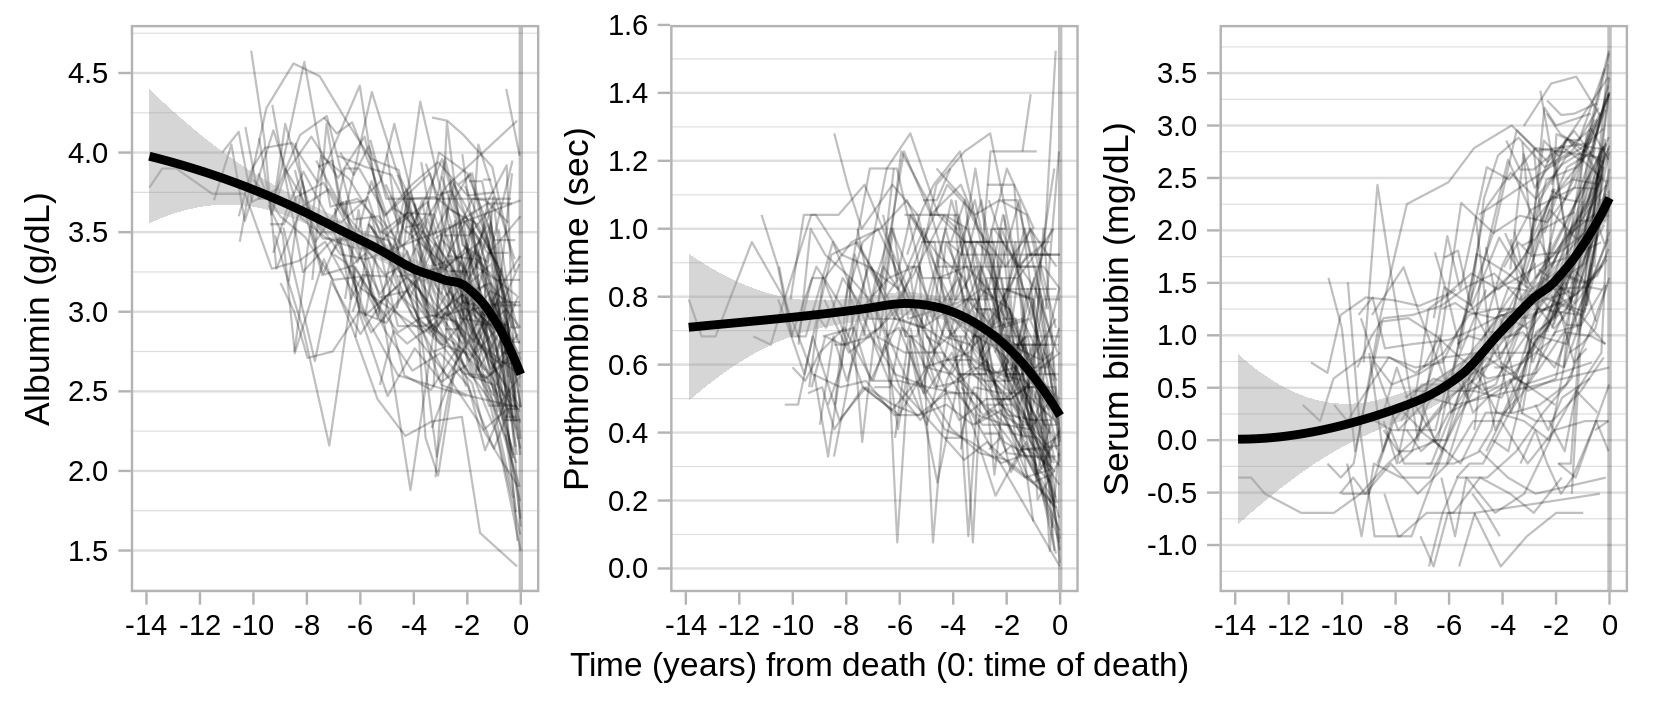
\includegraphics{Figures_Chapter1/PBCtrajectories.png}
      \caption{Longitudinal trajectories for three chosen biomarkers from PBC data. Grey lines show individual trajectories and overlaid smoothed (LOESS) curves the average trajectories for those who experienced mortality during follow-up and those who did not.}
      \label{fig:PBCtrajectories}
  \end{figure}
  
  %\resettocmain
  \section{Thesis outline}\label{sec:intro-thesis-outline}
  % One line introduction -->
  With an overview of joint modelling and its development in literature provided in Sections \ref{sec:jointintro} and \ref{sec:intro-evolution-parent}, we proceed by presenting the structure of the thesis on a chapter-by-chapter basis.
  
  % `Classic' methods -->
  In Chapter \ref{cha:methods-classic}, we lay the foundations for the thesis by first establishing the notation to be used throughout. We then introduce the multivariate extension of the `classic' joint models, which are our specific models of interest, elucidating parameters of interest as well as the estimation routine. Couched in a semiparametric maximum likelihood approach we provide an overview of the EM algorithm, aligning our methodology with  `classic' literature. Stemming from this approach, we introduce numerical integration methods. We further outline how one can `complete' inference and obtain standard errors for a fitted joint model. Finally, we offer a comprehensive overview of simulating data within the joint modeling framework; a crucial technique for the forthcoming chapters.
  
  % Approximation -->
  In Chapter \ref{cha:approx}, we draw attention to the computational burden which precludes, or makes overtly cumbersome, estimation for multivariate joint models by maximum likelihood. We introduce a normal approximation first proffered by \citet{Bernhardt15}, with details of this approximate EM algorithm provided; the approximation is used exhaustively throughout the thesis. Extensive simulation results are given, which serve to showcase the performance of the algorithm. Additionally, we offer comparison in terms of computation time as well as parameter estimates with existing software which is similar in its estimation approach.

  % GMVJM -->
  In Chapter \ref{cha:flexible} we continue utilising the approximate EM algorithm but extend the longitudinal sub-model to the non-Gaussian case; the idea being that many clinical data will not be continuous, or the Gaussian assumption not otherwise appropriate. We consider five different exponential families and provide an overview of the estimation procedure required for these so-called `generalised' multivariate joint models in a similar spirit to Chapter \ref{cha:approx}. Once more we provide multitudes of simulation study results to exhibit performance of the approximate EM algorithm.

  % Justification -->
  Owing to its large-scale use in the thesis it is of considerable importance to thoroughly investigate, understand, and justify the normal approximation. In Chapter \ref{cha:justification}, beginning with its foundations before delineating strategies to justify said approximation, we seek to achieve this; swathes of results are provided along with interpretation.

  % Post-hoc analyses -->
  We then shift focus to avenues for analysis of a fitted joint model. That is, with the methodology outlined in Chapters \ref{cha:methods-classic}--\ref{cha:flexible}, what can one \textit{do} with the fitted joint model: Does it fit the data well? How can it be used for predictions? Such questions are answered in Chapter \ref{cha:posthoc} where we collate post-hoc analyses, from defining residuals for the two processes, to outlining how one can bridge from a joint model to a predictive one.

  % PBC application -->
  Chapter \ref{cha:app-PBC} can be viewed as something of an amalgamation of Chapters \ref{cha:methods-classic}, \ref{cha:approx}, \ref{cha:flexible}, and \ref{cha:posthoc}. We seek to provide an extensive application to the motivating set of clinical data from Section \ref{sec:intro-motivation-pbc}: The aim of the chapter is to identify, and perform post-hoc analyses on, the `best-fitting' (multivariate) joint model for the data.  

  % Conclusions/Future work and appendices -->
  Finally, the thesis is brought to a close by our conclusions along with discussions of possible future research avenues in Chapter \ref{cha:conclusion}. The thesis is supplemented by Appendices \ref{cha:appendix-ExtraStuff}--\ref{cha:appendix-supplementary-figures} which house an assortment of extra derivations and results (both tabulated and graphical). Furthermore Appendix \ref{cha:appendix-gmvjoint} provides a brief overview of the \tt{R} package built alongside the work in Chapter \ref{cha:flexible}, \tt{gmvjoint} \citep{Murray2023}, which is used to obtain \textit{all results} presented in the thesis.
\end{chapter} 
  \begin{chapter}{\label{cha:methods-classic}The Classic Joint Modelling Framework}
In this chapter, the multivariate joint modelling framework under which we operate is defined, along with requisite notation. Following this we detail parameter estimation via maximum likelihood and data simulation techniques for the constituent sub-models as well as the joint model itself. We note that we present the `\textit{classic}' joint model in the first instance, named as such since early literature exclusively considered responses which were assumed Gaussian. In Chapter \ref{cha:flexible} we relax this assumption and introduce a breadth of other response types and in Chapter \ref{cha:posthoc} explore avenues for post-hoc analyses and prediction.
  \section{\label{sec:methods-jm}Joint modelling}
  \subsection{\label{sec:methods-notation}Models, likelihood and notation}
  For each subject $i=1,\dots,n$ we observe $\Y=\lb\Y{_1}^\top,\dots,\Y{_K}^\top\rb^\top$ where each $\Y{_k}, k=1,\dots,K$ denotes the $\kth$ longitudinal response of interest $\Y{_k}=\lb y_{i1k},\dots,y_{im_{ik}k}\rb^\top$. Each of the $K$ responses are measured $m_{ik}$ times, which can differ between subjects and responses. We observe a (possibly right-censored) event time $T_i=\min(T_i^*,C_i)$ where $T_i^*$ denotes the true event time and $C_i$ the independent potential censoring time, subsequently introducing failure indicator $\Delta_i$ which is unity if $T_i^*<C_i$ and zero otherwise.
  
  We adopt the following linear mixed effects model for the $\kth$ longitudinal response
  \begin{equation}
    \begin{aligned}
      \Y{_k} &= \X_{ik}\lb t\rb\bb_{k} + \Z_{ik}\lb t\rb\b{_k} + \bm{\varepsilon}_{ik}\\
      \b{_k} &\sim N_{q_k}\lb 0, \mathrm{D}_k\rb, \qquad \bm{\varepsilon}_{ik}\sim N\lb0, \sigma^2_{\varepsilon_k}\rb,\qquad \b{_k}\indep\bm{\varepsilon}_{ik},
    \end{aligned}
  \label{eq:methods-lmm}
  \end{equation}
  Here, $\X_{ik}$ denotes the (possibly time-dependent) design matrix for the fixed effects of interest to the $\kth$ longitudinal response for subject $i$ with corresponding $p_k$-vector of coefficients $\bb_k$. Likewise, $\Z_{ik}$ is a (possibly time-dependent) random effects design matrix and $\b{_k}$ the subject-specific $q_k$-vector of random effects. These random effects are assumed to follow a zero-mean multivariate normal distribution with covariance matrix $\mathrm{D}_k$. Across the $K$ longitudinal responses, we establish collections of the fixed effects $\bb=\lb\bb_1^\top,\dots,\bb_K^\top\rb^\top$ as well as the random effects $\b=\lb\b{_1}^\top,\dots,\b{_K}^\top\rb^\top$ for subject $i$.
  
  We form the joint model by inducing an association between the $K$ longitudinal trajectories and the hazard $\li$ through inclusion of the random effects $\b{_k}$. The sub-model for the event-time process is the usual Cox proportional hazards (PH) model
  \begin{align}
       \lambda_i(t)=\lambda_0(t)\exp\lbr\bm{S}_i^\top\bm{\zeta} + \Sk\gamma_k\bm{W}_k(t)^\top\b{_k}\rbr.
  \label{eq:methods-survival}
  \end{align}
  Here $\K$ is the vector of baseline covariates of interest to the event-time process and $\bz$ the corresponding $p_s$--vector of coefficients. The baseline hazard $\lo(\cdot)$ is treated as a nuisance parameter and left unspecified. Parameter $\gamma_k$ represents the strength of association between the random effects for the $\kth$ longitudinal response in \eqref{eq:methods-lmm} and the hazard, with $\bm{W}_k(t)$ denoting the appropriate vector function of time corresponding to the random effects structure on the $\kth$ longitudinal response. This could take the form of an intercept and slope, natural cubic splines and so on. As an example, consider $K=2$ responses, the first modelled under an intercept and slope specification and the other by random intercept only, the exponent in \eqref{eq:methods-survival} becomes $\exp\lbr\bm{S}_i^\top\bm{\zeta} + \gamma_1\lb1, t\rb^\top\lb b_{i10} b_{i11}\rb + \gamma_2b_{i20}\rbr$. One interprets $\gamma_k$ as any parameter in a Cox model: Larger values increase the (log) hazard whereas smaller values decrease it. If $\gamma_k$ is not significantly different from the null, then a separate analysis would suffice.  

  It is equally -- if not more -- popular in literature to define the nature of the association in \eqref{eq:methods-survival} by the current value of the $\kth$ linear predictor, rather than only its random effects (see \eg Table 1 in \citet{Hickey2016}), as was discussed in Section \ref{sec:intro-evolution-REs}. We elect the shared random effects association structure out of preference alone; deviations away from some population mean trajectory being the driving force behind an observed association. More complex association structures could include stationary Gaussian processes \citep{Henderson2000, Martins2022}, or current-value-and-slope parameterisations \citep{Rizopoulos2011B, Rustand2023}. 
  
  \subsection{\label{sec:methods-likelihood}Likelihood}
  As we exclusively consider estimation via (semiparametric) maximum likelihood, we first define the log-likelihood of the joint distribution of the set of observed outcomes for subject $i$, $\lbr\Y{_1},\dots,\Y{_K},T_i,\Delta_i\rbr$. In doing so, we assume that each longitudinal process and the survival process are conditional on the random effects $\b$: The correlation between measurements in the $\kth$ longitudinal process as well as the association between this longitudinal process and the event-time process are accounted for by the random effects. We define the joint density as 
  \begin{equation}
      f\lb T_i, \Delta_i, \Y|\b;\bO\rb = f\lb T_i,\Delta_i|\b;\bO\rb f\lb\Y|\b;\bO\rb
  \label{eq:methods-cond-indep}
  \end{equation}
  where $f\lb\Y|\b;\bO\rb=\prod_{k=1}^Kf\lb\Y{_k}|\b{_k};\bO\rb$ can be thought of as i.e. the product of the individual probability density functions (pdf) for the $K$ longitudinal processes and $f(T_i,\Delta_i|\b;\bO)$ denotes the pdf for the event-time process. The vector of parameters is denoted by $\bO$. We then define the observed data likelihood for subject $i$ as
    \begin{align}
    f\lb T_i, \Delta_i, \Y; \bO\rb &= \int_{-\infty}^\infty f\lb T_i, \Delta_i, \Y, \b; \bO\rb d\b \nonumber \\
    &= \int_{-\infty}^\infty\ls\prod_{k=1}^Kf\lb\Y{_k}|\b{_k};\bb_k,\sigma_k\rb\rs f\lb T_i,\Delta_i|\b;\bg,\bm{\zeta}\rb f\lb\b|\mathrm{D}\rb d\b.
    \label{eq:methods-obs-likelihood}
    \end{align}
  where we have integrated out the unobserved random effects. We have additionally introduced $\bg=\lb\gamma_1,\dots,\gamma_K\rb^\top$ as the vector of association parameters across the $K$ responses. We now explicitly define the parameter vector $\bO=\lb\vech\lb\mathrm{D}\rb^\top,\bb^\top,\bg^\top,\bz^\top\rb^\top$, where $\vech(\cdot)$ denotes the half-vectorisation of its matrix argument, thus returning all unique elements.
  
  Since we seek to maximise the log-likelihood $\ell(\bO)=\Si\log f\lb T_i, \Delta_i, \Y; \bO\rb$, we present the logarithm of each constituent density in \eqref{eq:methods-obs-likelihood}. The log-likelihood of the random effects density is given by the multivariate normal 
  \begin{equation}
      \log f\lb\b|\mathrm{D}\rb=-\frac{q}{2}\log(2\pi)-\frac{1}{2}\log|\mathrm{D}|-\frac{1}{2}\b^\top\mathrm{D}^{-1}\b,
  \label{eq:methods-loglik-ranefs}
  \end{equation}
  where $q$ denotes the dimensionality of the random effects covariance matrix $\mathrm{D}$ i.e. $q=\Sk q_k$ and $|M|$ denotes the determinant of matrix $M$. The event-time process has log-likelihood
  \begin{equation}
    \begin{aligned}
        \log f\lb T_i,\Delta_i|\b;\bg,\bm{\zeta}\rb &= \Delta_i\log\lo\lb T_i\rb + \Delta_i\ls\K^\top\bm{\zeta} + \Sk\gamma_k\bm{W}_k(T_i)^\top\b{_k}\rs \\
        & \qquad \quad - \int_0^{T_i}\lo\lb u\rb\exp\lbr\K^\top\bm{\zeta}+ \Sk\gamma_k\bm{W}_k(u)^\top\b{_k}\rbr \mathrm{d}u,
    \end{aligned}
  \label{eq:methods-loglik-survival}
  \end{equation}
  herein, the vector function of time corresponding to the specification of the $\kth$ random effects, $\bm{W}_k(\cdot)$ introduced in \eqref{eq:methods-survival}, is employed with associated failure time $T_i$, as well as with each survived failure time in the integrand. Notably under an unspecified baseline hazard $\lo\lb\cdot\rb$ the quantity in the integrand in \eqref{eq:methods-loglik-survival} is only non-zero \textit{at} the observed failure times \citep{Henderson2000}.
  
  Finally, we consider the the log-likelihood of the longitudinal processes. We first exploit the fact that we believe each of the $K$ responses to be (multivariate) normal, conditional on the random effects. For each subject $i$ we construct block-diagonal matrices across the $K$ longitudinal responses for the covariate information, $\mathrm{X}_i=\dsum\mathrm{X}_{ik}$; the random effects structure $\mathrm{Z}_i=\dsum\mathrm{Z}_{ik}$ and error terms $\mathrm{V}_i=\dsum\sigma^2_{\varepsilon_k}\mathbb{I}_{m_{ik}}$. Here, $\mathbb{I}_{x}$ denotes the $x\times x$ identity matrix and $\bigoplus$ denotes the direct matrix sum of its arguments. The log-likelihood for the longitudinal responses is then 
  \begin{align}\label{eq:methods-loglik-longit}
    \log f(\Y|\b;\bO) &= -\frac{m_i}{2}\log(2\pi)-\frac{1}{2}\log|\mathrm{V}_i|-\frac{1}{2}\lb\Y-\bm{\eta}_i\rb^\top\mathrm{V}_i^{-1}\lb\Y-\bm{\eta}_i\rb,\\
    \bm{\eta}_i &= \mathrm{X}_i\bb-\mathrm{Z}_i\b, \nonumber
  %\label{eq:methods-loglik-longit}
  \end{align}
  where $m_i=\Sk m_{ik}$ .  
  
\section{\label{sec:methods-estimation-EM}Parameter estimation via the EM algorithm}
As we discussed in Section \ref{sec:jointintro}, initial approaches to fitting joint models were in the form of two-stage approaches. Whilst these were simple to implement, they were found in many instances to produce biased parameter estimates (see e.g. \citet{Sweeting2011}). We therefore focus on estimation via (semiparametric) maximum likelihood, as was undertaken in seminal underpinning literature \citep{Wulfsohn97, Henderson2000}. Maximisation of $\ell(\bO)=\Si\log f\lb T_i, \Delta_i, \Y; \bO\rb$ with respect to $\bO$ in this frequentist framework is traditionally undertaken by usage of the Expectation Maximisation (EM) algorithm.
\subsection{\label{sec:methods-em-general}A general overview of the EM algorithm}
  In situations where a procedure for maximum likelihood estimation would be possible if not for the absence of some data, the EM algorithm has arisen as a popular, broadly applicable algorithm that provides an iterative procedure for computing said MLEs. The underlying idea of the EM algorithm is to construct the \textit{complete} data likelihood -- which allows for MLEs to be found iteratively -- given an \textit{incomplete} data problem \citep{Mclachlan08}.
  
  Let $f(\bm{Y}=\bm{y};\bO)$ be the probability density function (pdf) of the observed data vector $\bm{y}$. We henceforth view the observed data $\bm{y}$ as being incomplete, and a function of the complete data vector $\bm{x}$; more formally we have mapping from sample spaces $\mathcal{X}$ to $\mathcal{Y}$. We note that the concept of \textit{incomplete} data covers not only the `conventional' notion of missing data but additionally when some variable(s) would not be observable in practicality.\newline
  We introduce next the pdf for the complete data $f_c(\bm{X}=\bm{x};\bO)$, where the subscript $c$ is used to differentiate this from the above pdf for the observed data, and signifies `complete'. The complete data log-likelihood, if $\bm{x}$ were observable, is $\ell_c(\bO)=\log f_c(\bm{x};\bO)$. However, instead of observing the complete data $\bm{x}\in\mathcal{X}$, we observe the incomplete data $\bm{y}=\bm{y}(\bm{x})\in\mathcal{Y}$ as detailed previously. It follows that \citep{Mclachlan08}
  \begin{align*}
      f(\bm{y};\bO)=\int_{\mathcal{X}(\bm{y})}f_c(\bm{x};\bO)d\bm{x}.
  \end{align*}
  The EM algorithm essentially seeks to solve the incomplete data likelihood equation $\pt\ell(\bO)/\pt\bO=\bm{0}$ by instead using the complete data log-likelihood $\ell_c(\bO)$, which in practise is replaced by its conditional expectation on the observed data $\bm{y}$ at the current estimate of parameter vector $\bO$, at say iteration $m$. The EM algorithm consists of two `steps' per iteration which are eponymous to the approach: The expectation (E-) and maximisation (M-) step. On the $(m+1)$st iteration, the E-step and M-step are defined as:
  \begin{description}
  \item [E-step] Calculate 
  \begin{equation}
      Q\lb\bO;\bO^{(m)}\rb=\Exp\!\ls\ell_c(\bO)|\bm{y};\bO^{(m)}\rs.
  \label{eq:em-gen-estep}
  \end{equation}
  
  \item [M-step] Maximise $Q\lb\bO;\bO^{(m)}\rb$ with respect to $\bO$, i.e.
  \begin{align}
      \bO^{(m+1)}=\underset{\bO}{\arg\max}\ Q\lb\bO;\bO^{(m)}\rb.
  \label{eq:em-gen-mstep}
  \end{align}
  \end{description}
  To elucidate further; each EM iteration requires conditional expectations of the form $\mathbb{E}\ls g(\bm{x})|\bm{y};\bO\rs$, where $g(\bm{x})$ is some function on the complete data required to form the maximum likelihood update in the M-step, which one obtains through e.g. score equations.
  
 \subsection{\label{sec:jm-em-jm}The EM algorithm in a joint modelling framework} 
  With the constituent E- and M-steps laid out in \eqref{eq:em-gen-estep} and \eqref{eq:em-gen-mstep}, respectively, we can turn attention toward parameter estimation for the observed data likelihood \eqref{eq:methods-obs-likelihood}. \newline
  The set of \textit{observed} data for subject $i$ is constructed by the longitudinal response(s), $\Y$, the subject's event time $T_i$ and failure indicator $\Delta_i$: $\lbr\Y,T_i,\Delta_i\rbr$. To be explicit, the \textit{complete} data for subject $i$ is $\lbr\Y,T_i,\Delta_i,\b\rbr$ whereby every element except for the random effects $\b$ are observed. These random effects are then treated as \textit{missing data} upon implementation of the EM algorithm.
  
  The E-step \eqref{eq:em-gen-estep} in the context of a joint model at iteration $(m+1)$ is
  \begin{align*}
    Q\lb\bO;\bO^{(m)}\rb&=\Si\Expi{\log f(\Y, T_i, \Delta_i, \b|\bO)}\\
    &=\sum_{i=1}^n\int_{-\infty}^\infty\lbr\log f(\Y, T_i, \Delta_i, \b|\bO)\rbr f\big(\b|\Y,T_i,\Delta_i;\bO^{(m)}\big)d\b,
  \end{align*}
  where the integrand provides the contribution to the expected complete data (log) likelihood by subject $i$. The expectation $\Exp_i\ls\cdot\rs$ is taken with respect to the conditional distribution of the random effects on the observed data at a current set of parameter estimates $f(\b|\Y,T_i,\Delta_i;\bO^{(m)})$. The expected value of the complete data log-likelihood (which forms this E-step) is
  \begin{equation}
    \begin{aligned}
      Q\lb\bO;\bO^{(m)}\rb&=\Si \Exp_i\!\bigg[\log f\lb\Y|\b;\bO^{(m)}\rb + \log f\lb T_i,\Delta_i|\b;\bO^{(m)}\rb \\&\qquad\qquad\qquad+ \log f\lb\b|\bO^{(m)}\rb\bigg].
    \end{aligned}
  \label{eq:methods-E-step}
  \end{equation}
  The M-step is formed by maximising $n$ \textit{sets} of conditional expectations of the form $\mathbb{E}_i[g\lb\b\rb|T_i,\Delta_i,\Y;\bO]$ found in the preceding E-step, where $g\lb\b\rb$ denotes some necessary function of the random effects and the expectation is calculated against the conditional distribution $f\big(\b|\Y,T_i,\Delta_i;\bO^{(m)}\big)$. 
  
  The form of the parameter updates in the M-step are widely reported in literature, each illustrating the form required of $g\lb\b\rb$ in the preceding E-step. Here, the updated parameter estimates $\bO^{(m+1)}$ are given using the `current' estimates from the previous iteration, $\bO^{(m)}$:
  \begin{equation}
  \begin{aligned}
    \bb^{(m+1)} &= \lb\Si\X_i^\top\X_i\rb^{-1}\lb\Si\X_i^\top\lb\Y-\Z_i \Expi{\b}\rb\rb;\\
    \sigma_k^{2^{(m+1)}} &=\frac{1}{\Si m_{ik}}\Si \Exp_i\!\ls\lb\Y{_k}-\X_{ik}\bb{_k}^{(m)}-\Z_{ik}\b{_k}\rb^\top
                                 \lb\Y{_k}-\X_{ik}\bb{_k}^{(m)}-\Z_{ik}\b{_k}\rb\rs;\\
    \mathrm{D}^{(m+1)} &= \frac{1}{n}\Si \Expi{\b\b^\top};\\
    \lambda^{(m+1)}_0(t) &= \frac{\Si\Delta_i \mathrm{I}(T_i=t)}{\Si \Exp_i\!\ls\exp\lbr\K^\top\bz^{(m)}+\Sk\gamma_k^{(m)}\bm{W}_k\lb t\rb^\top\b{_k}\rbr\rs \mathrm{I}(T_i>t)};
  \end{aligned}
  \label{eq:methods-classicMstep}
  \end{equation}
  
  where $I\lb\cdot\rb$ is the indicator function. The update for the parameters associated with the survival (log) density \eqref{eq:methods-loglik-survival}, $\bg$ and $\bz$, do not exist in closed form (owing to their housing in an exponent), so are maximised iteratively by a one-step Newton Raphson algorithm. We let $\bm{\Phi}=\lb\bg^\top,\bz^\top\rb^\top$ denote the survival parameters, with update from iteration $(m)$ to $(m+1)$ given by
  \begin{equation}
      \bm{\Phi}^{(m+1)}=\bm{\Phi}^{(m)}-\ls\Si\mathrm{H}_i\lb\bm{\Phi}^{(m)}\rb\rs^{-1}\ls\Si s_i\lb\bm{\Phi}^{(m)}\rb\rs,
  \label{eq:methods-survMstep}
  \end{equation}
  where $s_i\lb\bm{\Phi}\rb$ is the gradient vector of the conditional expectation of the requisite complete data (profile) log-likelihood with respect to $\bm{\Phi}$, and $\mathrm{H}_i\lb\bm{\Phi}\rb$ the matrix of second derivatives for subject $i$.
  We undertake a more in-depth look at the E-step for these joint models in the next section.
  \section{The E-step for joint models}\label{sec:methods-Estepdetails}
  We require expectations of the form 
  \begin{equation*}
      \Expi{g\lb\b\rb|T_i, \Delta_i, \Y; \bO},
  \end{equation*}
  which are taken with respect to the density of the random effects conditioned on the observed data at the current set of parameter estimates, with this `current set' notation temporarily dropped,
  \begin{equation}
      \Expi{g\lb\b\rb|T_i, \Delta_i, \Y; \bO}=\int_{-\infty}^\infty g\lb\b\rb \condb d\b.
  \label{eq:numint-target}
  \end{equation}
  In the presence of the random effects $\b$ the longitudinal process(es) $\Y$ \textit{do not} inform the survival process $\mathcal{S}_i=\lbr T_i,\Delta_i\rbr$; these are conditionally independent given $\b$. With this in mind we then slightly rewrite our conditional density $\condb$ to be
  \begin{align*}
    f\lb\b|\cS;\Y,\bO\rb
  \end{align*}
  where the set of survival information $\cS$ is momentarily used for ease of presentation, and $\Y$ is now treated as an extraneous element.

  We then proceed using Bayes' theorem to rewrite this conditional density 
  \begin{align}
    f\lb\b|\cS;\Y,\bO\rb=\frac{f\lb\cS|\b;\Y,\bO\rb f\lb\b|\Y,\bO\rb}{f\lb\cS|\Y,\bO\rb},
  \label{eq:numint-condb-step}
  \end{align}
  where the quantity $f\lb\b|\Y,\bO\rb$ is given in terms of the conditional and marginal probabilities
  \begin{align}
    f\lb\b|\Y,\bO\rb=\frac{f\lb\Y,\b|\bO\rb}{f\lb\Y|\bO\rb}=\frac{f\lb\Y,\b|\bO\rb}{\int_{-\infty}^\infty f\lb\Y,\b|\bO\rb d\b}\equiv
    \frac{f\lb\Y|\b;\bO\rb f\lb\b|\bO\rb}{\int_{-\infty}^\infty f\lb\Y|\b;\bO\rb f\lb\b|\bO\rb d\b},
  \label{eq:numint-problem}
  \end{align}
  Rewriting the denominator in \eqref{eq:numint-condb-step} with effort taken to remove the conditioning of $\cS$ on $\Y$ we obtain
  \begin{align*}
    f\lb\cS|\Y,\bO\rb=\int_{-\infty}^\infty f\lb\cS|\b;\bO\rb f\lb\b|\Y,\bO\rb d\b.
  \end{align*}

  Thus, the density against which expectations are evaluated is (returning to our previously-used notation)
  \begin{equation}
    \condb=\frac{\sfT\bY}{\int_{-\infty}^\infty\sfT\bY d\b},
  \label{eq:numint-expandtarget}
  \end{equation}
  with all required expectations then taking the form
  \begin{equation}
    \begin{aligned}
        \Expi{g\lb\b\rb|T_i,\Delta_i,\Y;\bO}&=\frac{1}{\int_{-\infty}^\infty\sfT\bY d\b}\\
        &\qquad\qquad\qquad\times\int_{-\infty}^\infty g\lb\b\rb\sfT\bY d\b.
    \end{aligned}    
  \label{eq:numint-form-of-expectation}
  \end{equation}
  For the case when the conditional distribution of $\Y|\b$ is assumed to be multivariate normal i.e.\ $\Y|\b\sim N\lb\X_i\bb+\Z_i\b,\mathrm{V}_i\rb$, the density $f\lb\b|\Y;\bO\rb$ present in \eqref{eq:numint-condb-step} and, by extension, \eqref{eq:numint-form-of-expectation} is given by multivariate normal theory \citep{Wulfsohn97, Lin2002, Hickey2018}
  \begin{equation}
      \b|\Y;\bO\sim N\lb\mathrm{A}_i\lbr\Z_i^\top\mathrm{V}_i^{-1}\lb\Y-\X_i\bb\rb\rbr, \mathrm{A}_i\rb,
  \label{eq:b-cond-mvn}
  \end{equation}
  where $\mathrm{A}_i=\lb\Z_i^\top\mathrm{V}_i^{-1}\Z_i + \mathrm{D}^{-1}\rb^{-1}$. This tractable expression for $\bY$ allows us to avoid the computational burden of evaluating \eqref{eq:numint-problem}.

\subsection{Numerical integration}\label{sec:numint-intro}
Fitting joint models can be computationally burdensome, owing in large part to the integral taken over the random effects in calculation of the necessary conditional expectations \eqref{eq:numint-target}, which are necessary in obtaining the parameter estimates at each subsequent M-step \eqref{eq:methods-classicMstep}. 

This integral does not have an analytic solution; a numerical approach is typically employed to approximate these integrals for each subject. Such evaluation over the random effects serves as the main source of computational woe, and is the main bottleneck in the majority of cases. The random effects are likely not one-dimensional, and computational demand is commensurate with their dimensionality \citep{Philipson2020}.

Several methods for approximation of the conditional expectation \eqref{eq:numint-target} are found in the literature. Early methods included low-dimensional Gauss-Hermite quadrature or Monte Carlo methods \citep{Wulfsohn97, Henderson2000}; both since becoming routinely used in available software. More recently, adaptive quadrature methods have been employed, along with Laplace approximations. In the following sections, we seek to outline how these methods are used in the E-step of a joint model to evaluate $\Expi{g\lb\b\rb|T_i, \Delta_i, \Y; \bO}$.
\subsection{Gauss-Hermite quadrature}\label{sec:numint-GH}
Gauss-Hermite quadrature is a method for approximating definite integrals of the form
\begin{equation*}
  \int_{-\infty}^\infty f(x)\exp\lbr-x^2\rbr dx.
\end{equation*}
Since the integrand above resembles the normal distribution, Gauss-Hermite quadrature is particularly useful for approximating integrals resembling the normal kernel. Considering our expectation of interest, which we restate from \eqref{eq:numint-target}
\begin{align*}
    \Expi{g\lb\b\rb|T_i, \Delta_i, \Y; \bO}=\int_{-\infty}^\infty g(\b) f\lb\b|T_i,\Delta_i, \Y;\bO\rb d\b,
\end{align*}
under `standard' Gauss-Hermite quadrature rules we evaluate the above by the sum of $\varrho$ weighted evaluations of the integrand at pre-specified abscissae. The weights $\bm{w}$ and abcissae $\bm{v}$ are available in numerous locations, including the \tt{R} package \tt{statmod} \citep{quadrature}. The integral is approximated then by
\begin{align}
    \int_{-\infty}^\infty g\lb\b\rb &f\lb\b|T_i,\Delta_i,\Y;\bO\rb d\b \approx \nonumber\\
    & 2^{q/2}\sum_{l_1=1}^\varrho\dots\sum_{l_q=1}^\varrho w_l g\lb \bm{v}_l\sqrt{2}\rb f\lb \bm{v}_l\sqrt{2}|T_i,\Delta_i,\Y;\bO\rb\exp\lbr||\bm{v}_l||^2\rbr,
\label{eq:numint-standardGH}
\end{align}
where $||x||$ denotes the euclidean norm of its argument. In \eqref{eq:numint-standardGH} above, the abscissae $\bm{v}_l=\lb v_{l_1}, \dots, v_{l_q}\rb^\top$ each have corresponding weights $\bm{w}=\lb w_1,\dots,w_\varrho\rb^\top$. That is, we extend a univariate Gaussian quadrature rule to the $q$-dimensioned case \citep{RizopoulosJMbook}.

Owing to how the specific values of the nodes and weights are assigned to best interpolate a polynomial of degree $2\varrho-1$, the closeness of the approximation \eqref{eq:numint-standardGH} to the exact value improves as $\varrho$ increases. Typically, this `standard' Gauss-Hermite method assumes zero-centering with the shape of a normal distribution. Therefore, another important factor that affects the quality of the approximation is the location of the quadrature points with respect to the modal mass of the integrand. That is, the approximation \eqref{eq:numint-standardGH} will be poor if most of the mass of $g\lb\b\rb\!f\lb\b|T_i,\Delta_i,\Y;\bO\rb$ lies away from zero, and/or the spread of this integrand is different from the weight function. In the context of (generalised) linear mixed models, \citet{Stringer2022} argue that this `shifting' of mass occurs with some regularity.

This `standard' Gauss-Hermite quadrature provides then a method to (essentially, exactly with large enough $\varrho$) appraise integrals whose analytic solution is either non-existent, or irritating, to calculate. We draw attention to two main drawbacks to the approach. First, the computational burden of the dimension of the random effects coupled with requirement of a potentially high number of quadrature points being necessary to achieve an approximation of sufficient accuracy. Secondly, one will obtain a poor approximation if the mass of the objective function is located away from zero, and so a more reliable method may be desired. 

Indeed, in much of the early literature surrounding joint models, strides were taken away from this numerical integration method in favour of Monte Carlo methods (which we go on to discuss in Section \ref{sec:numint-MC}) perhaps because of these issues. In the next section, we examine a method which attempts to circumvent possible malposition of the quadrature routine. 

\subsection{Adaptive Gauss-Hermite quadrature}\label{sec:numint-aGH}
With consternation surrounding the position of quadrature nodes we outlined in the previous section in mind we explore now an `adaptive' quadrature rule \citep{Pinheiro1995}. This aims to appropriately center and scale abscissae used in evaluation of the integrand \eqref{eq:numint-target}. The integral is approximated by
\begin{align}
    \int_{-\infty}^\infty g\lb\b\rb &f\lb\b|T_i,\Delta_i,\Y;\bO\rb d\b \approx \nonumber\\
    & 2^{q/2}|\hat{\mathrm{C}}_i|\sum_{l_1=1}^\varrho\dots\sum_{l_q=1}^\varrho w_l g\lb \hat{\bm{v}}_l\rb f\lb \hat{\bm{v}}_l|T_i,\Delta_i,\Y;\bO\rb\exp\lbr||\bm{v}_l||^2\rbr,
\label{eq:numint-aGH}
\end{align}
where the aforementioned shift in abcissae is performed by introduction of the term $\hat{\bm{v}}_l=\hat{\bm{b}}_i+\sqrt{2}\hat{\mathrm{C}}_i\bm{v}_l$, with $\bm{v}_l$ previously defined in addition to
\begin{align}
    \hb &= \arg\!\max{}\!_{\b}\lbr\log f\lb\Y, T_i, \Delta_i, \b;\bO\rb\rbr, \label{eq:argmaxb}\\
    \hat{\mathrm{H}}_i&=-\frac{\pt^2\log f\lb\Y, T_i, \Delta_i, \b;\bO\rb}{\pt\b\pt\b^\top}\bigg\rvert_{\b=\hb}. \label{eq:Hessb}
\end{align}
Finally, the term $\hat{\mathrm{C}}_i$ present in \eqref{eq:numint-aGH} is the lower triangular Choleski factorisation which satisfies $\hat{\mathrm{C}}_i\hat{\mathrm{C}}_i^\top=\hat{\mathrm{H}}_i^{-1}$. \citet{RizopoulosJMbook} draw attention to the transformed integrand resembling a $N\lb\bm{0},\frac{1}{2}\mathbb{I}_q\rb$ distribution; proportional to the weight function of Gauss-Hermite quadrature.

Since the evaluation \eqref{eq:numint-aGH} centers the abscissae $\bm{v}$ at the mode $\hb$ and scales by the curvature $\hat{\mathrm{H}}_i$ of the complete data (log) likelihood for each of the $n$ subjects, it generally provides a very good approximation of \eqref{eq:numint-target} \citep{Stringer2022}. Typically, this adaptive quadrature rule requires fewer abscissae than its `standard' counterpart explored in Section \ref{sec:numint-GH} \citep{RizopoulosJMbook}, owing to its eponymous `adaptive' quality.

Briefly, on the topic of the number of abscissae, we note little guidance within joint modelling literature for a proposed value for $\varrho$; simply that increasing it will likely stabilise parameter estimates. Couched in a GLMM setting, \citet{Stringer2022} recommend setting the number of quadrature points based on two characteristics of the data: The number of `groups' in the data (e.g. the number of subjects $n$) and the smallest number of observations across all $n$ groups $M=\min\lb m_i\rb$
\begin{align}
    \varrho_{{}_\mathrm{Stringer}} = \left\lceil\frac{3}{2}\log_{M}\!n-2\right\rceil.
\label{eq:numint-stringerRecc}
\end{align}

\subsection{Pseudo-adaptive Gauss-Hermite quadrature}\label{sec:numint-paGH}
Belying the promise of greater accuracy and fewer requisite abscissae in the routine outlined in \eqref{eq:numint-aGH}, large computational cost can manifest due to necessary \textit{repeated} calculation of $\hb$ and subsequently $\hat{\mathrm{H}}_i$, given in \eqref{eq:argmaxb} and \eqref{eq:Hessb}, respectively. Explicitly, since \eqref{eq:numint-aGH} is housed within the EM algorithm, both $\hb$ and $\hat{\mathrm{H}}_i, i=1,\dots,n$ need to be obtained at \textit{each} iteration, prior to whatever (potentially expensive) quadrature routine is undertaken.

To circumvent the repeated obtention of $n$ sets of this vector mode and its Hessian matrix, \citet{Rizopoulos2012} highlight that the (log) density $\log f\lb\Y,T_i,\Delta_i;\bO\rb$ is dominated by the (log) density associated with the linear mixed effects model $\log f\lb\Y|\b;\bO\rb$, which resembles the shape of some multivariate normal distribution. They argue then that the centering and scaling of abscissae for each individual need only be carried out once, prior to commencement of any EM algorithm. In a (very) similar fashion to \eqref{eq:numint-aGH}, we approximate
\begin{align}
    \int_{-\infty}^\infty g\lb\b\rb &f\lb\b|T_i,\Delta_i,\Y;\bO\rb d\b \approx \nonumber\\
    & 2^{q/2}|\tilde{\mathrm{C}}_i|\sum_{l_1=1}^\varrho\dots\sum_{l_q=1}^\varrho w_l g\lb \tilde{\bm{v}}_l\rb f\lb \tilde{\bm{v}}_l|T_i,\Delta_i,\Y;\bO\rb\exp\lbr||\bm{v}_l||^2\rbr.
\label{eq:numint-paGH}
\end{align}
Here, $\tilde{\bm{v}}_l=\tilde{\bm{b}}_i+\sqrt{2}\tilde{\mathrm{C}}_i\bm{v}_l$ and $\tilde{\mathrm{C}}_i$ is the lower Choleski of $\tilde{\mathrm{H}}_i^{-1}$, where
\begin{align}
    \tilde{\bm{b}}_i=\arg\!\max{}\!_{\b}\lbr\log f\lb\Y, \b;\bO\rb\rbr, 
\label{eq:pargmaxb}
\end{align}
and $\tilde{\mathrm{H}}_i$ subsequently defined in a corresponding way to \eqref{eq:Hessb}, with the log density $\log f\lb\Y,\b;\bO\rb$ at mode $\tilde{\bm{b}}_i$. Given the aforementioned domination of the complete data log-density by the log-density contributed by the linear mixed model, \citet{Rizopoulos2012} propose, under general regularity conditions,
\begin{equation}
    \log f\lb\b|T_i,\Delta_i,\Y;\bO\rb\overset{\mathrm{P}}{\rightarrow}N\lb\tilde{\bm{b}}_i,\tilde{\mathrm{H}}_i^{-1}\rb.
\label{eq:rizappx}
\end{equation}

With this `pseudo-adaptive' method laid out, an immediately obvious advantage is the elusion of repeated (re-)calculation of abscissae for the sample at each EM iteration; compounded by the ease at which \textit{both} $\tilde{\bm{b}}_i$ \textit{and} $\tilde{\mathrm{H}}_i,\ \forall\ i=1,\dots,n$ can be obtained by readily-available software (e.g. \tt{nlme} \citep{R-nlme}, \tt{lme4} \citep{R-lme4}), with such routines very often used in obtaining initial conditions for $\bO$. This, along with the `adaptive' routine outlined in Section \ref{sec:numint-aGH}, which acts as the foundation for \textit{this} routine, necessitating fewer quadrature points than the `standard' (Section \ref{sec:numint-GH}), results in this `pseudo-adaptive' quadrature method an attractive avenue. 

We note that although \eqref{eq:numint-aGH} and \eqref{eq:numint-paGH} reduce the number of abscissae required to reliably approximate the integral, the number of evaluations they necessitate still increases exponentially with the dimension of the integrand determined by the number of random effects $q$.

\subsection{Monte Carlo methods}\label{sec:numint-MC}
Monte Carlo integration is perhaps an obvious alternative to these quadrature methods, as it provides a probabilistic representation of the integral \eqref{eq:numint-target} \citep{Lemieux2009}. In Section \ref{sec:methods-Estepdetails}, we showed that the conditional expectation $\Expi{g\lb\b\rb|T_i, \Delta_i, \Y; \bO}$ can be written as
\begin{align}
    \Expi{g\lb\b\rb|T_i, \Delta_i, \Y; \bO}=\frac{\int_{-\infty}^\infty g\lb\b\rb f\lb T_i,\Delta_i|\b;\bO\rb f\lb\b|\Y;\bO\rb d\b}{\int_{-\infty}^\infty f\lb T_i,\Delta_i|\b;\bO\rb f\lb\b|\Y;\bO\rb d\b}.
\label{eq:numint-fullcondexp}
\end{align}
where the density $f\lb T_i,\Delta_i|\b;\bO\rb$ is known from \eqref{eq:methods-loglik-survival} and, operating under an assumption of multivariate normality in $\Y|\b$, the density $f\lb\b|\Y;\bO\rb$ can be calculated from multivariate normal theory, as given in \eqref{eq:b-cond-mvn}. 

Monte Carlo integration can therefore be used to approximate \eqref{eq:numint-fullcondexp} by first sampling $N$ realizations from \eqref{eq:b-cond-mvn} for each subject and then calculating the ratio of sample mean values for the numerator and denominator integrands present in \eqref{eq:numint-fullcondexp}. That is,
\begin{align}
    \Expi{g\lb\b\rb|T_i, \Delta_i, \Y; \bO}\approx\frac{\frac{1}{N}\sum_{l=1}^N g\lb\b^{(l)}\rb f\lb T_i,\Delta_i|\b^{(l)};\bO\rb}{\frac{1}{N}\sum_{l=1}^Nf\lb T_i,\Delta_i|\b^{(l)};\bO\rb}.
\label{eq:numint-MC}
\end{align}
To be explicit, the draws $\b^{(l)},\ l = 1,\dots,N$ are sampled from the multivariate normal distribution given in \eqref{eq:b-cond-mvn} using, for instance, \tt{rmvnorm} available in package \tt{mvtnorm} \citep{R-mvtnorm} or \tt{mvrnorm} from package \tt{MASS} \citep{R-MASS}. 

\citet{Henderson2000} utilised antithetic Monte Carlo sampling to halve the number of samples required, producing $N$ negatively correlated sample pairs; the negative correlation between these pairs leading to smaller variance in the sample means in \eqref{eq:numint-MC}. It is worth mentioning that there is little guidance available with respect to a tactful choice of $N$. \citet{Philipson2020} outline in greater detail these properties, and additionally draw attention to quasi-Monte Carlo methods for sampling of $\b|\Y;\bO$ couched within the E-step of a joint model. 

Notably, Monte Carlo methods do not suffer the same curse of dimensionality as quadrature: The integral approximation given in \eqref{eq:numint-MC} does \textit{not} directly depend on $q$. However, the random samples from the distribution of $\b$ may themselves become computationally prohibitive at larger $q$.
  
  \section{Calculation of standard errors}\label{sec:methods-SEs}
  With our maximum likelihood estimates $\hbO$ obtained from an EM algorithm as delineated in Sections \ref{sec:methods-estimation-EM} and \ref{sec:methods-Estepdetails}, we now turn attention to obtaining standard errors (SEs) for the MLEs in order to `complete' inference for the fitted joint model. Doing so allows us the form the usual Wald confidence intervals for the parameter estimates, obtain $p$-values, and so on. Generally, standard errors are found by inversion of the information matrix, $\mathcal{I}\big(\hbO\big)$. 
  
  The lack of \textit{automatic} provision of $\cal I$ by the EM algorithm lead to several proffered methods to calculate, or approximate, the \textit{observed} information matrix, $\mathcal{I}_o\big(\hbO\big)$. Instead of surveying the general-case methods laid out in \citet{Mclachlan08}, we focus here on outlining methods for estimating standard errors using the EM algorithm for the joint model specifically.

  \citet{Hsieh2006} highlight the major challenge with standard error estimation for joint models is presence of the unspecified (\ie non-parametric) baseline hazard $\lo\lb\cdot\rb$, so the standard asymptotic properties for the MLE $\hbO$ afforded by the EM algorithm do not apply. In Section \ref{sec:jm-em-jm} we therefore essentially considered the \textit{profile} likelihood in parameter updates. This profile likelihood with nonparametric MLE $\hat{\lambda}_0$ shouldn't be dependent upon $\lo$. However, \citet{Hsieh2006} admonish that this is \textit{not} the case, since the estimate for $\lambda_0\lb\cdot\rb$ appearing in \eqref{eq:methods-classicMstep} holds implicit membership in $\bO$ upon which the distribution of the random effects is conditionally dependent in \eqref{eq:numint-form-of-expectation} \ie itself involves the density $f\lb T_i,\Delta_i|\b;\bg,\bz,\lo\rb$.

  In light of the challenges stemming from the unspecified $\lo$, we present three methods for calculation of SEs. We explore the bootstrap, and two methods which attempt to approximate $\mathcal{I}_o\big(\hbO\big)$ in the next sections. We do not compute the standard errors for the baseline hazard $\hat{\lambda}_0$ in all simulations and applications in proceeding chapters: Its high dimensionality, determined by the number of unique event times, could lead to instability in any obtained information matrix, and, moreover, they are likely not of interest considering $\lo$ is set as a nuisance parameter at the outset.
  
  \subsection{The bootstrap}\label{sec:methods-SE-bootsrap}
  In a scenario where establishing a handle on uncertainty in parameter estimates is supposedly not clear or straight-forward, bootstrapping is perhaps an obvious choice. Consider having the `original' joint model which is fit to the set of observed data constructed by available measurements for $n$ subjects, $\mathcal{D}=\lbr\mathcal{D}_1,\dots,\mathcal{D}_n\rbr$ where $\mathcal{D}_i=\lbr T_i, \Delta_i, \bm{Y}_i\rbr$. Subsequently, we sample with replacement across the \textit{subjects}, such that for each bootstrap replicate $b=1,\dots,N$ we obtain a set of `new' data denoted $\mathcal{D}^{(b)}$. It is important to emphasise that the sampling is done over the subjects, and not individual data points which one may carry out in the case of ungrouped data. For each set of `new' data, we obtain $\hbO^{(b)}$ by fitting a joint model to said data. Sample quantities of interest (median value, standard deviation, 95\% CI etc.) can then be trivially found by calculation over the $N$ sets of bootstrapped MLEs.
  
  Despite ease of carrying out the bootstrap method, there are several reasons why this avenue is unattractive. Firstly, bootstrapping will obviously be a slow method, and $N$ typically needs to be quite large, with its computation time dependent on the time taken for the EM algorithm itself. However \citet{Hickey2018} point out simply starting the EM algorithm on resampled data at the the MLEs obtained by the joint model fit to the original data lessens this burden. Secondly, there are no guarantees that resampling won't produce a problematic set of data which could lead to convergence problems in the EM algorithm. Finally both \citet{Hsieh2006} and \citet{Xu2014} note that the bootstrap method overestimated the standard errors in the joint model.
  
  \subsection{Observed empirical information matrix}\label{sec:methods-SE-obsemp}
  \citet{Hickey2018} approximate the so-called observed empirical information matrix $\mathcal{I}_e$ to obtain SEs for $\hbO$. After convergence of the EM algorithm, we have the vector of parameter estimates \textit{and} the estimates for the unspecified baseline hazard $\hat{\lambda}_0\lb t\rb$. Using the Breslow estimator for the baseline hazard given in \eqref{eq:methods-classicMstep}, we calculate
  \begin{equation}
      \mathcal{I}_e\big(\hbO\big)=\lbr\Si s_i\big(\hbO\big)s_i^\top\big(\hbO\big)\rbr-n^{-1}S\big(\hbO\big) S^\top\big(\hbO\big),
  \label{eq:methods-obsemp}
  \end{equation}
  where $s_i\big(\hbO\big)$ denotes the gradient vector of the conditional expectation of complete data (profile) log-likelihood function \eqref{eq:methods-E-step} evaluated at $\hbO$ \ie the score statistic and $S\big(\hbO\big)=\sum_is_i\big(\hbO\big)$. We note that whilst the bootstrap surveyed in the previous section is known to \textit{overestimate} the standard errors, those produced by the approximation of the information matrix here are known to \textit{underestimate} the uncertainty in our parameter estimates owing to the usage of the profile log-likelihood outlined previously in the obtention of score vectors  \citep{Hsieh2006}.
  \subsection{Numerical differentiation of the Fisher score}\label{sec:methods-SE-xu2014}
  \citet{Xu2014}, like the method outlined in the previous section, seek to approximate $\mathcal{I}_o$, and provide four methods based on numerical differentiation to do so. All four presented use either the forward differencing method, or the Richardson extrapolation. Said differentiation is carried out on either the M-step update \eqref{eq:em-gen-mstep} or the Fisher score vector of the complete data log-likelihood; in both cases a profile technique is used. Owing to its similarity with the method shown in Section \ref{sec:methods-SE-obsemp}, we present only the approach using the profile Fisher score vector and present numerical differentiation techniques in Appendix \ref{sec:appendix-numdiff}.

  Essentially, \citet{Xu2014} recommend that for each element of $\hbO$ which undergoes perturbation in the numerical differentiation routine of choice, the baseline hazard is then re-maximised at this perturbed vector, and the differentiation of this profile Fisher score carried out as normal. Therefore, computational expense is related to the number of parameters and/or the number of random effects as well as the choice of differentiation routine. After convergence, we have the vector of MLEs $\hbO$ which has length
  \begin{equation}
      L=\mathrm{len}\big(\hbO\big)=\frac{q\lb q+1\rb}{2}+p_1+\dots+p_K+p_s+K,
  \label{eq:methods-length-of-omega}
  \end{equation}
  determined by the joint model specification. In order to obtain the standard errors of $\hbO$ by the method in \citet{Xu2014} we perturb, in turn, each of the $l=1,\dots,L$ parameters under the numeric differentiation routine. For each perturbation per parameter, we re-calculate the baseline hazard $\hat{\lambda}^{(l)}_0$, and evaluate the profile Fisher score at this $l^{\mathrm{th}}$ perturbed vector, thereby obtaining the $l^{\mathrm{th}}$ column in the approximated $\mathcal{I}_o$, which is then formed `over' the numerical differentiation routine. This method of obtaining SEs is notably less computationally expensive under forward differencing, since only one perturbation occurs, compared to the four undertaken by the Richardson extrapolation.
  
  \section{\label{sec:methods-simulation}Simulation}
  Simulation studies are important statistical tools: Investigating performance properties and adequacy of statistical models in pre-specified situations. We briefly illustrate how we undertake simulation for the longitudinal and survival sub-models before outlining how we simulate data under the `combined' joint modelling framework. The method(s) outlined are then carried forward in all simulated datasets used. In practice we employ bespoke code which allows for fine-tuning of simulation scenarios we present. 
  
  The remainder of this section briefly outlines data simulation under a linear mixed model; simulation of event times; and simulation under the joint modelling framework. We bring the chapter to a close by outlining numerous considerations one may take into account when simulating the data under a joint model.
  
  \subsection{\label{sec:sim-longit}Simulating the longitudinal response}
  Simulation of a response under a linear mixed effects model \eqref{eq:methods-lmm} is relatively straight-forward. For some candidate parameter vector $\bO_{\D,\bb,\sigma^2_\varepsilon}^{(\mathrm{TRUE})}=\lb\vech\lb\D\rb^\top,\bb^\top,\sigma^2_\varepsilon\rb^\top$, which denotes the `true' values of the necessary parameters, we carry out the following steps:
  \begin{enumerate}
      \item Simulate the random effects $\b$ for all $n$ desired subjects. In practise, the function \tt{mvrnorm} from the \tt{R} package \tt{MASS} \citep{R-MASS} is used with zero-mean and the positive semi-definite covariance matrix $\D$ supplied.
      \item Define the design matrices $\X_i$ and $\Z_i$. For all simulations, $\X_i$ is defined -- unless otherwise stated -- as the matrix formed by the horizontal concatenation of an intercept, the vector of follow-up times, a single standard normal deviate and a single Bernoulli draw ($p=0.5$). We define the vector of follow-up times for each subject as $\bm{t}_i=\lb0,\dots,\kappa\rb$ with $\kappa$ the maximal follow-up time. The vector $t_i$ is regularly spaced according to the length of the profile $r$. Both $\kappa$ and $r$ are controlled in simulations. The specification of $\Z_i$ is simulation dependent: For instance if a random intercept and slope random is desired, then it is defined as the horizontal concatenation of the intercept column and $\bm{t}_i$.
      \item Define $\bm{\eta}_i=\X_i\bb+\Z_i\b$ and simulate $\Y$ using \tt{rnorm} with mean $\bm{\eta}_i$ and standard deviation $\sqrt{\sigma^2_\varepsilon}$.
  \end{enumerate}
  The above steps then produce $n$ sets of $r$-vectors of the simulated Gaussian response. That is, $\Expi{\Y|\b;\bO_{\D,\bb,\sigma^2_\varepsilon}^{(\mathrm{TRUE})}}$ is conditionally (multivariate) normal. One can then trivially extend this to produce $K$ vectors with differing \eg fixed effects. In circumstances where the response one wishes to simulate is non-Gaussian, then some requisite inverse-link function is used on $\bm{\eta}_i$, as we go on to detail in Chapter \ref{cha:flexible}. 
  
  Of course, these $r$-vectors of response(s) are truncated at the subject's simulated event time in the joint model setting. We outline methodology to simulate failure times in the general case in the next section and under a joint model in Section \ref{sec:sim-joint}.

  \subsection{\label{sec:sim-survtime}Simulation of survival times}
  Cox proportional hazards regression is the ubiquitous approach to modelling the effect of a the covariate vector $\bm{S}_i$ on the hazard of some time-to-event outcome. Simplifying the Cox PH regression model \eqref{eq:methods-survival} to the usual $\lambda_i\lb t|\bm{S}_i\rb=\lambda_0(t)\exp\lbr \bm{S}_i^\top\bz\rbr$, with $\lo(t)$ and $\bz$ previously defined in Section \ref{sec:methods-notation}. The survival function, which gives probability that subject $i$ survives past time $t$ is then $S(t)=\exp\ls-\Lambda_0(t)\exp\lbr\bm{S}_i^\top\bz\rbr\rs$, where $\Lambda_0=\int_0^t\lo(u)du$ denotes the cumulative baseline hazard. The distribution of survival times under this Cox PH regression is then $F\lb t|\bm{S}_i\rb=1-S(t|\bm{S}_i)$. \citet{Bender2005} demonstrate that one can simulate the true event time of subject i by
  \begin{align*}
      T_i^*=\Lambda_0^{-1}\ls-\log U\exp\lbr-\bm{S}_i^\top\bz\rbr\rs,\quad U\sim\text{Unif}\lb0,1\rb.
  \end{align*}
  Therefore, survival times can be generated for any baseline hazard which has an invertible cumulative baseline hazard function $\Lambda$: \citet{Bender2005} noted that only the exponential, Weibull and Gompertz baseline hazard functions satisfy not only this criterion, but additionally share the assumption of proportional hazards with the Cox PH model. The formula required for simulation of survival times for each of these three candidate distributions are given in Table \ref{tab:simulation-parameterisation}
  \begin{table}[t]
      \centering
      \rowcolors{2}{lightgray!20}{white}
      \small
      \begin{tabular}{lcr}
           Distribution & Parameter(s) & Formula for simulation \\ \midrule
           Exponential  &  Scale $\nu>0$ & $T_i^*=-\frac{\log U}{\nu\exp\lbr\bm{S}_i^\top\bz\rbr}$\\
           Weibull & Scale $\nu>0$, shape $\alpha>0$ & $T_i^*=\lb-\frac{\log U}{\nu\exp\lbr\bm{S}_i^\top\bz\rbr}\rb^{1/\alpha}$\\
           Gompertz &  Scale $\nu>0$, shape $-\infty<\alpha<\infty$ & $T_i^*=\frac{1}{\alpha}\log\ls1-\frac{\alpha\log\lb U\rb}{\nu\exp\lbr\bm{S}_i^\top\bz\rbr}\rs$
      \end{tabular}
      \caption{Simulation of event times for a given subject $i$ under the exponential, Weibull and Gompertz distributions. $U$ denotes a uniform draw in each case and $\bm{S}_i$ is subject $i$'s vector of baseline covariates.}
      \label{tab:simulation-parameterisation}
  \end{table}
  \newline Going forward, owing to its wide use in survival analysis, we use the Gompertz as our baseline hazard of choice. The simulated event time $T_i^*$ is given by
  \begin{align}
      T_i^*=\frac{1}{\alpha}\log\ls1-\frac{\alpha\log\lb U\rb}{\nu\exp\lbr\bm{S}_i^\top\bz\rbr}\rs,\quad U\sim\text{Unif}\lb0,1\rb,
  \label{eq:sim-bender}
  \end{align}
  where $\alpha$ and $\nu$ are the shape and scale, respectively, of the Gompertz distribution. As was the case for simulation of the longitudinal process in Section \ref{sec:sim-longit}, we are able to fine-tune the survival process by choice of parameter $\bz$, in addition to the underlying baseline hazard by $\nu$ and $\alpha$, which are defined for the Gompertz distribution in Table \ref{tab:simulation-parameterisation}. This fine-tuning is done \textit{independently} of the longitudinal process at this stage; we consider simulation under the joint modelling framework proper in the next section. 
  
  We note in passing that another way to simulate $T_i^*$ is to directly solve the survival function $S\lb t\rb$ for each subject given their covariates $\bm{S}_i$ via a root-finding algorithm (such as \tt{uniroot} in base \tt{R}); a useful alternative if the distribution of interest is non-invertible or the baseline hazard is otherwise specified. 
  
  \subsection{\label{sec:sim-joint}Simulation under a joint modelling framework}
  Advantages of using Cox PH regression are its ability to incorporate both (a): Time-varying covariate effects, that is, a covariate whose value is fixed at baseline, but effect on the hazard is time-varying; and (b): Time-varying covariates, that is a covariate whose value changes over time, e.g. cumulative dosage received in a clinical trial \citep{Austin2012}. Under the Cox PH specification in the joint modelling framework with a random intercept-and-slope specification we indeed have a time varying covariate in the form of the $K$ slope terms across random effects $\b{_1}=\lb b_{i11}, b_{i21},\dots,b_{iK1}\rb^\top$ thereby falling into category (b). When a random intercepts-only structure is instead desired, the formulation \eqref{eq:sim-bender} suffices, with the term including covariate information expanded to include our association parameters and random intercept terms: $\exp\lbr\bm{S}_i^\top\bz+\Sk\gamma_kb_{ik0}\rbr$. 
  
  Given inclusion of random slope terms $\b{_1}$, we follow closely the work of \citet{Austin2012}, who expand work outlined in the previous section by \citet{Bender2005} to the case with such a time-varying covariate. Rewriting the Cox PH formulation \eqref{eq:methods-survival}
  \begin{equation}
  \begin{aligned}
      \lambda(t|\bm{S}_i,\b;\bz,\bg)=&\lo(t)\exp\lbr\lb\bm{S}_i^\top\bz+\Sk\gamma_kb_{ik0}\rb + 
      \lb\Sk\gamma_kb_{ik1}\rb t\rbr,\\
      \lambda(t|\cdot)=&\lo(t)\exp\lbr P + Qt\rbr
  \end{aligned}
  \label{eq:sim-rewrite}
  \end{equation}
  where we have collected time-invariant and time-varying terms together into the arbitrarily-named $P$ and $Q$, respectively. Then, given that the Gompertz baseline hazard is $\lambda_0(t)=\nu\exp\lbr\alpha t\rbr$, with shape $-\infty<\alpha<\infty$ and scale parameter $\nu>0$. We obtain from \eqref{eq:sim-rewrite},
  \begin{align*}
      \Lambda(t|\cdot)&=\intzt\lambda(u|\cdot)du=\intzt\exp\lbr P+Qu\rbr\nu\exp\lbr\alpha u\rbr du\\
      &=\nu\exp\lbr P\rbr\intzt\exp\lbr (Q + \alpha)u\rbr du\\
      &=\nu\exp\lbr P\rbr\ls\frac{1}{Q + \alpha}\exp\lbr\lb Q + \alpha\rb u\rbr\rs^t_0\\
      \Lambda(t|\cdot)&=\frac{\nu\exp\lbr P\rbr}{Q + \alpha}\ls\exp\lbr\lb Q+\alpha\rb t\rbr-1\rs.
  \end{align*}
  Then, setting the survival function $S(t)$ equal to a random uniform draw, $U$, and rearranging for $t$ we obtain
  \begin{align*}
      U&=S\lb t\rb=\exp\lbr-\frac{\nu\exp\lbr P\rbr}{Q + \alpha}\ls\exp\lbr\lb Q + \alpha\rb t\rbr-1\rs\rbr\\
      \exp\lbr\lb Q + \alpha\rb t\rbr&=1-\frac{\nu\exp\lbr P\rbr}{Q + \alpha}\log U\\
      \implies t&=\log\lb1-\frac{Q + \alpha}{\nu\exp\lbr P\rbr}\log U\rb\bigg /\lb Q + \alpha\rb.
  \end{align*}
  Finally then, our true event time $T_i^*$ can be generated by
  \begin{equation}
      T_i^*=\simsurvofrac\log\ls1-\frac{(Q+\alpha)\log U}{\nu\exp\lbr P\rbr}\rs,\quad U\sim\text{Unif}\lb0,1\rb,
  \label{eq:sim-jm}
  \end{equation}
  where $P$ and $Q$ are defined in \eqref{eq:sim-rewrite}. Similar derivations for Weibull and exponential baseline hazards are given in Appendix \ref{sec:appendix-survtimes}. 

  In addition to the survival time as outlined in this section and the last, we additionally generate $n$ censor-times, $C_i\sim\mathrm{Exp}\lb \Upsilon\rb$ where $\Upsilon$ denotes the rate parameter; representing yet more control over the simulated data. With both what is the `true' failure time $T_i^*$ and censor time $C_i$ simulated, we set each observed event time $T_i=\min\lb T_i^*,C_i\rb$ and generate $\Delta_i$ accordingly. If $T_i>\kappa$ then it is truncated to value $T_i=\kappa+0.1$ for analysis purposes and $\Delta_i$ is set to zero. The baseline covariates used in simulating the failure time for subject $i$ throughout the thesis are the same single standard normal and Bernoulli draws obtained in Section \ref{sec:sim-longit}. 
  
  \subsection{Simulation beyond an intercept and slope structure\label{sec:sim-quad}}
  The mechanisms for simulation for a joint model under an intercept-only and intercept-and-slope random effects structure has been outlined in the previous section: The intercept-only random effects formulation is encapsulated in previous work by \citet{Bender2005} presented in \eqref{eq:sim-bender}, and the inclusion of a random slope in addition lead us to consider work by \citet{Austin2012} in treating these as time-varying covariates \eqref{eq:sim-jm}.
  
  However, simulations are also necessary when working with more complex random effects structures. For instance, under a quadratic formulation in the simulated response, or when spline terms are included with $M$ internal knots, taking form $\sum_{m=0}^M(\alpha_m+b_{im})B_m(t)$, where $\bm{\alpha}=\lb\alpha_0,\dots,\alpha_M\rb$ are B-spline coefficients and $\lbr B(t)\rbr$ the truncated linear basis (see e.g. \citet{Barrett2017} for a joint model with such a spline specification). Under such examples, the integration outlined in the previous section becomes awkward and unappealing, and so we utilise previously-used methods \citep{R-joineR} to generate data under more complex random effects structures.
  
  We expand the time-varying term $Q\rightarrow Q(\b, t)$ here to encapsulate any functional form of the random effects. For example, utilising a quadratic random effects structure arbitrarily across all $k$ responses results in 
  \begin{align*}
    Q(\b, t)=\Sk\gamma_k\lb b_{ik1}t+b_{ik2}t^2\rb, 
  \end{align*}
  and likewise any polynomial of order $p$ gives
  \begin{align*}
    Q(\b,t)=\Sk\gamma_k\lb b_{ik1}t+\dots+b_{ikp}t^p\rb    
  \end{align*}
  as well as \eg spline term(s). Given the definition of the hazard $\lambda(t|\cdot)$ is 
  \begin{align}
      \underset{\Delta t\rightarrow 0}{\lim}\frac{\Pr(t\le T\le t + \Delta t|T\ge t,\ \cdot)}{\Delta t},
  \label{eq:haz-def}
  \end{align}
  which we can trivially rearrange to
  \begin{align}
    \underset{\Delta t\rightarrow0}{\lim}\lambda(t|\cdot)\Delta t = 
    \underset{\Delta t\rightarrow0}{\lim}\Pr(t\le T\le t + \Delta t|T\ge t,\ \cdot),
    \label{eq:haz-def-dt}
  \end{align}
  with the hazard $\lambda(t|\cdot)$ given by \eqref{eq:sim-rewrite}. Therefore failure times, simulated under a host of random effects specifications given by $Q\lb\b,t\rb$, are available. 
  
  Choosing a nominally small value for $\Delta t$ allows us to generate a sufficiently fine grid which multiplies the hazard. This scaled hazard is equivalent to the probability of failure occurring in the fine-grid time interval $(t, t + \Delta t)$. We also generate a vector of possible times for each individual from time $0$ to the truncation time $\kappa$ with step-size $\Delta t$. Each of the generated probabilities can be compared to a $\text{Unif}\lb0,1\rb$ draw. If the probability does not exceed the uniform deviate then the survival time is set as $\kappa$, otherwise the survival time takes the value of the minimum candidate time (i.e. when the event first happened).
  
  To illustrate, consider subject $i$ with step-size $\Delta t=0.02$ and truncation time $\kappa=5$. We would generate vector of candidate times $\bm{t}=(0.00, 0.02,\dots,2.50,2.52,\dots,4.98,5.00)^\top$. The probability of an event occurring at each $t\in\bm{t}$ is then calculated, dependent on form of chosen $Q(\b,t)$. These probabilities are then compared against $\text{Unif}\lb0,1\rb$ realizations to obtain, say, $\bm{t}^*=(\kappa,\kappa,\dots,\kappa,2.52,\dots,4.98,\kappa)^\top$. The minimal value of $\bm{t}^*$ is then set as the true failure time for this subject, $T_i^*=2.52$. Subject $i$ additionally has censor-time simulated as outlined in Section \ref{sec:sim-joint}, which allows us to allocate $T_i$ in an identical manner.
  
  Although this methodology allows for a wide breadth of random effects structures, the use of potentially very large (owing to elected step-size) matrices can slow down data generation considerably. Additionally, the vector of candidate times $\bm{t}$ are effectively discrete times, which could have the effect of many subjects having the same simulated failure time, which could be troublesome in certain simulation scenarios. Of course, this could be circumvented by choosing a finer value for $\Delta t$, at greater computational cost.
  
  \section{\label{sec:sim-considerations}Simulation considerations}
  Simulation of survival times is a task which is hard to control with absolute perfection: More so an act of balancing several different aspects which come from the specification of parameters $\bg$ and $\bz$; the underlying Gompertz baseline hazard via scale and shape parameters $\nu$ and $\alpha$, respectively; as well as the magnitude of the random effects via their allocated variance in $\D$. A delineation of how these different facets -- which we control in simulation settings -- combine to allow one to obtain $n$ failure times time was given in Section \ref{sec:sim-joint}. In this section we consider these three factors which can alter both the incidence of failure in $[0,\kappa]$ as well as the distribution of simulated $T_i^*$.
  
  \subsection{The baseline hazard}\label{sec:sim-considerations-basehaz}
  We exclusively simulate under a Gompertz baseline hazard of the form $\lo(t)=\nu\exp\lbr\alpha t\rbr$. The scale parameter $\nu$ can be thought of as baseline hazard's intercept term: If the shape parameter $\alpha$ is zero then the baseline hazard is stationary through time, and values of $\gamma$ and $\zeta$ mainly drive the failure times with no inclusion of time itself contributing to the underlying baseline hazard. The shape parameter itself therefore allows the baseline hazard to increase or decrease over time.
  
  Setting the survival parameters to zero, such that they do not impact the hazard, we select a set of values for $\log\nu=\lbr-4,-3,-2,-1\rbr$ and $\alpha=\lbr-0.4, -0.2, 0.2, 0.4\rbr$ and simulate one hundred sets of data, collating the simulated failure times from each simulated data set. 
  
  Figure \ref{fig:sim-alphanu} shows the distribution of survival times under each combination of $\lbr\log\nu\rbr$ and $\lbr\alpha\rbr$ above. At lower values of $\log\nu$ we note the distribution of event times changes as $\alpha$ increases from a negative to positive value: Failures occur earlier on in follow-up (driven by $\log\nu$) with visible drop-off in frequency over time owing to the negative $\alpha$, and vice versa for $\alpha>0$.

  For $\log\nu>=-2$ this change in distribution is less pronounced owing to the underlying Gompertz baseline hazard (arising from this scale parameter) being already adequately high. The failure times are more concentrated around the start of simulated follow-up at largest $\alpha=0.4$, whereas for $\alpha=-0.4$ there is still a somewhat noticeable `tail' of failure times comparatively.
  \begin{figure}[t]
    \centering
    \includegraphics[width=140mm, height = 90mm]{Figures_Chapter2/alpha_nu_failure_corrections.png}
    \caption{Distribution of simulated survival times under different parameterisations of the Gompertz baseline hazard.}
  \label{fig:sim-alphanu}
  \end{figure}
  
  \subsection{Magnitude of survival parameters}\label{sec:sim-considerations-gammazeta}
  Next, we consider altering the magnitude and sign of the survival parameters. Specifically, we simulate a univariate model with candidate association parameters $\gamma=\lbr-1.0, -0.5, 0.0, 0.5, 1.0\rbr$ and the coefficient attached to the binary baseline covariate in the survival model, taking values $\zeta_2=\lbr-1.0, -0.3, 0.3, 1.0\rbr$. Across each of these combinations of $\lbr\gamma\rbr$ and $\lbr\zeta_2\rbr$, we hold the parameters controlling the baseline hazard constant at $\log\nu=-1$ and $\alpha = 0$ in order to simulate a time-invariant baseline hazard. The covariance matrix on the random effects is set as a diagonal matrix of dimension two. With these set out, we expect the changes in simulated failure time densities to be driven by the changing values of $\lbr\gamma\rbr$ and $\lbr\zeta_2\rbr$.
  
  Figure \ref{fig:sim-gammazeta} illustrates the effect of different magnitudes of $\gamma$ and $\zeta_2$. The effect of an increased $\zeta_2$ is perhaps best exemplified in the `column' for $\gamma = 0$. Here, we infer that the increasing value of $\zeta_2$ simply increases the underlying baseline hazard, illustrated by the greater incidence of failures due to said higher baseline hazard. Interestingly, the distribution of failure times for the positive-negative pairs of values for $\gamma$ are visually (almost) identical. This is due to the simulation of the random effects producing an approximate half-and-half `split' of those who are above the global trajectory (thus their hazard \textit{increases} with positive $\gamma$) and those below it (\textit{increasing} with negative $\gamma$). We see as $|\gamma|$ increases, more failures occur earlier in the period of follow-up, which is exacerbated by higher values of $\zeta_2$.
  \begin{figure}[t]
    \centering
    \includegraphics[width=140mm, height = 90mm]{Figures_Chapter2/gamma_zeta_failure2_corrections.png}
    \caption{Distribution of simulated survival times under different parameterisations of the survival parameters $\gamma$ and $\zeta_2$.}
  \label{fig:sim-gammazeta}
  \end{figure}
  
  \subsection{Magnitude of the random effects}\label{sec:sim-considerations-D}
  In a similar spirit to our investigation of the effect of survival parameter magnitude, we set the baseline hazard constant at $\log\nu=-1$ and $\alpha=0$. We hold the association parameter constant at a moderate $\gamma = 0.5$ and $\bz=\bm{0}$, such that failures occurring are likely to be due to ones deviation from a global trend, as dictated by the parameterisation of the covariance matrix $\mathrm{D}$. We set off-diagonal parameters $\mathrm{D}_{12}=\mathrm{D}_{21}=0$ and consider all $16$ possibilities for the diagonal of $\D$ from candidate intercept variances $\mathrm{D}_{11} = \lbr3.0, 1.0, 0.5, 0.5^2\rbr$ and slope variances $\mathrm{D}_{22} = \lbr1.0, 0.5, 0.25, 0.25^2\rbr$.
  
  Figure \ref{fig:sim-intslope} illustrates how the distribution of simulated survival times changes when the variance of random effects (thus the average magnitude of the random effects) increases. When the random effects can take larger values (\ie $D_{11}$ and/or $D_{22}$ are larger), an overall increase in the number of failure times as time progresses occurs. When the random intercept variance is greatest at $D_{11}=3$ the simulated failure times are most concentrated at start of follow-up occurs, especially when $D_{22}$ is comparatively smaller. Conversely, when random slope variance is greater, the distribution of simulated failure times have an elongated tail, demonstrating the impact of the simulated random slopes on the hazard.
  \begin{figure}[t]
    \centering
    \includegraphics[width=140mm, height = 90mm]{Figures_Chapter2/int_slope_failure.png}
    \caption{Distribution of simulated survival times under different magnitudes of random effect variance.}
  \label{fig:sim-intslope}
  \end{figure}

\end{chapter}
  \begin{chapter}{\label{cha:approx}Faster Fitting: An Approximate EM Algorithm}
\vfill
\begin{center}
    \begin{bluebox}
    The work presented in this chapter is based on the publication:\\Murray, J., Philipson, P., 2022. \textit{A fast approximate EM algorithm for joint models of survival and multivariate longitudinal data}. Computational Statistics \& Data Analysis 170, 107438. doi: \href{https://doi.org/10.1016/j.csda.2022.107438}{\tt{10.1016/j.csda.2022.107438}}.
    \end{bluebox}
\end{center}
\vfill
\clearpage
\section{Motivation}
In Chapter \ref{cha:methods-classic} we outlined the multivariate joint model framework with $K$ longitudinal responses which are assumed continuous and Gaussian. Available software for such joint models, representing existing computational approaches, was outlined in Sections \ref{sec:intro-evolution-multivariate} and \ref{sec:intro-evolution-software} encompassed both maximum likelihood approaches as well as the Bayesian paradigm.

Multivariate joint models (MVJMs) are superior to $K$ separate univariate fits, as they take into account the correlation \textit{between} the longitudinal responses; using all relevant information in the joint model thus obtaining correctly adjusted estimates for each response. Additionally, one obtains a single prediction using all possible information, rather than several from said $K$ univariate fits, each of which is likely to overstate the importance of any association when treated in isolation.

Fitting of these models is computationally burdensome, as mentioned in Section \ref{sec:numint-intro}, due to the multidimensional integral present in the E-step \eqref{eq:numint-target}.

\subsection{E-step constraints in multivariate joint models}\label{sec:approx-Estepmotiv}
As we outlined in Section \ref{sec:methods-Estepdetails}, and as alluded to above, most computational issues arise due the E-step \eqref{eq:methods-E-step}. Here necessary expectations are taken with respect to the distribution of the random effects conditional on the observed data at the current set of parameter estimates. Specifically, we require expectations of the form \eqref{eq:numint-target}, with this conditional distribution then having form \eqref{eq:numint-expandtarget}. However, owing to either an increased number of longitudinal responses in the multivariate joint model of interest; the complexity of their random effects structures; or both, existing techniques are likely to be less viable due to the inherent computational burden. This is to say, the existing methods we outlined in Sections \ref{sec:numint-GH}--\ref{sec:numint-MC} are likely to become infeasible as the dimension of the random effects, $q$, increases. Said intractability often manifesting itself by the computation time taken to fit these multivariate joint models being commensurate with $q$: Limiting the application of multivariate joint models to smaller numbers of random effects, longitudinal processes, or both. 

The different methods we outlined to evaluate integrals of interest in Sections \ref{sec:numint-aGH}--\ref{sec:numint-MC} in fact were all proposed in turn to overcome the apparent computational burden in earlier literature \eg \citet{Wulfsohn97}. Adaptive quadrature methods sought to reduce the number of weights and abscissae used in numerical integration, but the amount of evaluations may still be computationally demanding in spite of this, owing to large $q$. Monte Carlo methods themselves do not suffer the same burden, but may become prohibitive for higher dimensional random effects owing to the number of required samples for adequate evaluation. 

\citet{Hickey2018} go as far to speculate that inference for joint models with very many longitudinal responses, such as electronic healthcare records, may require some approximate method in evaluation of the integral \eqref{eq:numint-target} as part of parameter estimation under maximum likelihood.

\section{An approximate EM algorithm}\label{sec:approx-approx}
\subsection{A normal approximation}\label{sec:approx-approx-specificbit}
 \citet{Bernhardt15} proposed a normal approximation on the distribution of the random effects $\condb$ for each individual conditional on the observed data in the context of a joint model with a \textit{logistic} sub-model in place of the survival one \eqref{eq:methods-survival}. The proposed normal approximation has the effect of reducing the dimensionality of each required integral to be uniformally one, regardless of the complexity of the random effects. This then exploits that any linear combination of $\b$ would \textit{also} be normal, thereby improving computational efficiency. We seek then to extend their approximation to the joint model with a survival sub-model as introduced in the previous Chapter in Sections \ref{sec:methods-notation} and \ref{sec:methods-likelihood}.

 \citet{Bernhardt15} propose, at the parameter estimates at the current iteration $(m)$, $\tobm{\bO}$,
 \begin{align}
     \b|T_i,\Delta_i,\Y;\tobm{\bO},\tobm{\lo}\appx \Napprox,
 \label{eq:approx-approx}
 \end{align}
  where $\hb$ is the vector which maximises the complete data log-likelihood at the current set of parameter estimates:
  \begin{align}
      \hb=\argmax{\b}\log f\big(\b, T_i, \Delta_i, \Y; \tobm{\bO}\big);
  \label{eq:approx-bhat}
  \end{align}
  with estimated variance
  \begin{align}
      \hS=\lbr-\frac{\partial^2\log f\big(\b,T_i,\Delta_i,\Y;\tobm{\bO}\big)}{\partial\b\partial\b^\top}
    \bigg\rvert_{\b=\hb}\rbr^{-1}.
  \label{eq:approx-Sigmahat}
  \end{align}
  In \eqref{eq:approx-approx} we explicitly condition on the current estimate for the baseline hazard, $\tobm{\lo}$, which we treat as a nuisance parameter, holding \textit{implicit} membership in $\tobm{\bO}$ only. Hereafter, its involvement in the approximation and parameter estimates continues to be implicit in nature.
  
  It was previously demonstrated by \citet{Rizopoulos2012} that $f\lb\b|\Y;\bO\rb$ is approximately normal as $m_i\rightarrow\infty$ within the confines of a `classic' \textit{univariate} joint model. Subsequently, \citet{Bernhardt15} extended this to the multivariate Gaussian case we considered in Chapter \ref{cha:methods-classic} for the `full' conditional distribution shown in \eqref{eq:approx-approx}. We later devote Chapter \ref{cha:justification} to the justification of the above approximation.

  The approximation \eqref{eq:approx-approx} then allows for \textit{all} necessary conditional expectations which are of the form $\Expi{g\lb\b\rb|T_i, \Delta_i, \Y; \tobm{\bO}}$ to be taken with respect to a univariate normal distribution. Said normal distributions can then be quickly evaluated using adaptive Gauss-Hermite quadrature, which we outline in Section \ref{sec:approx-Mstep}. 

  \subsection{Starting values}\label{sec:approx-startvalues}
  The number of iterations required by the EM algorithm can be reduced by choosing starting values, $\bO^{(0)}$, which are close to the maximiser. We set about obtaining these initial values using pre-existing \tt{R} packages.
  
  For $k=1,\dots,K$ we obtain parameter estimates for the $\kth$ longitudinal process by fitting a linear mixed effects model using \tt{glmmTMB} \citep{R-glmmTMB}. This returns initial conditions for the fixed effects $\bb_k^{(0)}$ and the residual variance $\sigma_{\varepsilon_k}^{2^{(0)}}$. Additionally, we obtain the best linear unbiased predictors (BLUPs) for the random effects $\b{_k}$ along with their variance-covariance matrix $\D_k^{(0)}$. Then, across all $K$ responses we can construct the initial condition for the block-diagonal $\D^{(0)}=\dsum\D_k^{(0)}$, and populate the off-block-diagonal elements with $\mathrm{cov}\lb\bm{b}_e,\bm{b}_f\rb,\ e,f=1,\dots,K,\ e\neq f$.

  Next, we use the aforementioned BLUPs for each $k=1,\dots,K$ response, $\b{_k}$, as $K$ independent time-varying covariates in the usual Cox PH model, along with the time invariant $\bm{S}_i,\ i=1\dots n$, to obtain $\bm{\Phi}^{(0)}=\lb\gamma_1^{(0)},\dots,\gamma_K^{(0)},\bm{\zeta}^{(0)^{\top}}\rb^\top$. The form of each of these time-varying covariates is dependent upon the form of $\bm{W}_k(\cdot)$ in \eqref{eq:methods-survival} (\ie intercept and slope, quadratic specification and so on). This is done using the \tt{survival} package \citep{R-survival}, and additionally returns the initial estimate for the baseline hazard, $\lambda_0^{(0)}\lb\cdot\rb$.

  We can then form $\bO^{(0)}$ and go about parameter estimation via the EM algorithm, confident that it commences at parameter values which are conducive to faster convergence of the algorithm itself. We used \tt{glmmTMB} as it allows for efficient generalised mixed model fitting for numerous families, and we found it to provide much more stable parameter estimates in a more timely manner when compared with competing packages. Other packages, such as \tt{nlme} \citep{R-nlme} or \tt{lme4} \citep{R-lme4}, are very slightly quicker but restricted to modelling continuous (Gaussian) $\Y$, since we progress to considering non-Gaussian responses in Chapter \ref{cha:flexible}, we additionally use \tt{glmmTMB} here for simplicity. 
  
  \subsection{Convergence details}\label{sec:approx-convcrit}
  Posit that we have just completed one EM step from iteration $(m)$ to iteration $(m+1)$, and want to ascertain whether the algorithm has converged. Two standard rules for such an investigation are the absolute and relative convergence criteria -- the existing packages \tt{joineR} \citep{R-joineR} using the former and \tt{JM} \citep{R-JM} the latter -- for instance. 
  
  An issue one may encounter when attempting to maximise the likelihood via an iterative procedure such as EM is in becoming `stuck' near the maximiser, or prematurely declaring convergence to it. This can be remedied by taking into account the scale of parameters when applying these stopping rules: If a parameter is very small (\ie close to zero) in magnitude, it is perhaps likely that some numerical issue may come into play in calculation of the relative difference; likewise the absolute difference doesn't take into account the scale of parameters at all, and may prematurely stop the algorithm.

  One method to circumvent these potential issues is to employ a two-pronged approach: 
  \begin{align}
    \begin{cases}
        \max\lb|\tobmp{\Omega}_1-\tobm{\Omega}_1|,\dots,|\tobmp{\Omega}_L-\tobm{\Omega}_L|\rb&<\xi_1\ \mathrm{if}\ |\Omega_x| < \upsilon \\
        \max\lb\frac{|\tobmp{\Omega}_1-\tobm{\Omega}_1|}{|\tobm{\Omega}_1|+\nu},\dots, 
               \frac{|\tobmp{\Omega}_L-\tobm{\Omega}_L|}{|\tobm{\Omega}_L|+\nu}\rb&<\xi_2\ \underset{\!\!\!\!\!x=1,\dots,L}{\mathrm{if}\ |\Omega_x|\ge\upsilon}.
    \end{cases}
    \label{eq:approx-convcrit}       
  \end{align}
  where $L$ denotes the dimension of $\bO$ \eqref{eq:methods-length-of-omega}. Interestingly, this is the stopping rule used by the software \tt{SAS} in its EM algorithms; repurposed in the joint modelling setting recently by \tt{joineRML} \citep{Hickey2018}. 
  
  We opt for the convergence criterion shown above as the approach precludes issues one may encounter when considering solely one convergence criterion, whilst still affording accuracy in those parameters with estimates closer to zero; in particular those variance components on the diagonal of $\mathrm{D}$ that are bounded below by zero. In the relative difference criterion, $\nu$ is some small value added to the denominator to preclude numerical issues which might occur in the calculation here. In all presented simulations and analyses we use $\xi_1=\nu=10^{-3}$, $\xi_2 = 5\times10^{-3}$ and $\upsilon=0.1$ unless otherwise stated. 
 
  \subsection{The approximate EM algorithm}\label{sec:approx-approxEMalg}
  With details on how we obtain starting values and determine whether or not the model has converged, we now set out to illustrate how we utilise the approximation in Section \ref{sec:approx-approx-specificbit} within the context of an EM algorithm for a joint model. 
  
  In short, we obtain our initial conditions for the parameter vector $\bO$ and iteratively cycle between the E- and M-steps, refining these parameter estimates until convergence is deemed to have occurred. At \textit{each} iteration we utilise the approximation \eqref{eq:approx-approx}--\eqref{eq:approx-Sigmahat} to obtain conditional expectations before forming parameter updates; this specific process being elucidated in Section \ref{sec:approx-Mstep}. 
  
  With that being said, we lay out the general steps taken to fit MVJMs outlined in Section \ref{sec:methods-jm} in a similar spirit to existing work \citep{Bernhardt15, Murray2022, Murray2023}:
  \begin{enumerate}
      \item Employ the methodology outlined in Section \ref{sec:approx-startvalues} to obtain the initial conditions for the parameters, $\bO^{(0)}$.
      \item For any iteration $(m+1)$:
      \begin{enumerate}[label=\roman*.]
          \item Maximise $\log f\big(\b,T_i,\Delta_i,\Y;\tobm{\bO}\big)$ using the \tt{optim} function with the quasi-Newton BFGS algorithm to obtain $\hb$ and $\hS$ (see \eqref{eq:approx-bhat} and \eqref{eq:approx-Sigmahat}, respectively).
          \item Use the approximation \eqref{eq:approx-approx} to update the parameter vector $\tobm{\bO}\rightarrow\tobmp{\bO}$; greater detail is provided in Section \ref{sec:approx-Mstep}.
      \end{enumerate}
      \item Check whether the algorithm has converged by evaluating the convergence criterion \eqref{eq:approx-convcrit}. If the criterion is satisfied, exit the algorithm; otherwise, proceed to the next iteration by setting $(m)\rightarrow (m+1)$.
      \item Repeat steps 2. and 3. for a minimum of four iterations, cycling between parameter updates and convergence checks.
  \end{enumerate}
  
  \subsection{Standard error calculation}\label{sec:approx-SEs}
  In Section \ref{sec:methods-SEs} we explored three methods to calculate standard errors in order to complete inference. There, we posited that the approximation of the observed empirical information matrix \eqref{eq:methods-obsemp} would likely be preferable from a computational standpoint: It offers a route to obtain the standard errors in a more timely manner than by bootstrapping or repeated numerical differentiation.

  The observed empirical information matrix \eqref{eq:methods-obsemp} is calculated by $n$ subject specific score vectors evaluated at the MLEs $\hbO$

  \begin{equation}
    \begin{aligned}
        s_i\big(\hbO\big)=\int_{-\infty}^\infty\bigg[
                        \frac{\pt}{\pt\hbO}\bigg\{&\log f\big(\Y|\b;\hbO\big)+\log f\big(T_i,\Delta_i|\b;\hbO\big) \\&\qquad\qquad\qquad+ \log f\big(\b|\hbO\big)\bigg\}
                    \bigg] f\big(\b|T_i,\Delta_i,\Y;\hbO\big) d\b,
    \end{aligned}
  \label{eq:approx-score-equation}
  \end{equation}
  wherein, given the approximate method outlined in \ref{sec:approx-approx-specificbit}, the expectation presented above is taken with respect to the normal distribution in \eqref{eq:approx-approx}.

  Specifically, after convergence of the EM algorithm, we find $\hb$ and $\hS$ at the purported MLEs, $\hbO$. Then, the (profile) score vector \eqref{eq:approx-score-equation} is calculated. The constituent densities herein are conditionally independent given the random effects $\hb$, therefore we form `individual' constituent scores to form the score vector 
  \begin{equation*}
      s_i\big(\hbO\big)=\lb s_i\big(\hbO_\D\big)^\top, s_i\big(\hat{\bb}\big)^\top, s_i\lb\hat{\sigma}^2_{\varepsilon_1}\rb, \dots, s_i\lb\hat{\sigma}^2_{\varepsilon_K}\rb, s_i\big(\hat{\bm{\Phi}}\big)^\top\rb^\top,
  \end{equation*}
  wherein $\hbO_\D\equiv\vech\big(\hat{\D}\big)$. The constituent scores are given as (for simplicity's sake, the hat notation is momentarily dropped):
  \begin{equation}
      \begin{aligned}
          s_i\lb\bO_\D\rb&=-\frac{1}{2}\mathrm{Tr}\lb\D^{-1}\dXdY{\D}{\bO_\D}\rb+\frac{1}{2}\mathrm{Tr}\lb\D^{-1}\dXdY{\D}{\bO_\D}\D^{-1}\Expi{\tcrossprod{\b}}\rb;\\
          s_i\lb\bb\rb&=\X_i^\top\mathrm{V}_i^{-1}\lb\Y-\X_i\bb-\Z_i\Expi{\b}\rb;\\
          s_i\lb\sek\rb&=-\frac{m_{ik}}{2\sek}+\frac{\Expi{\lb\Y-\X_i\bb-\Z_i\b\rb^\top\lb\Y-\X_i\bb-\Z_i\b\rb}}{2\sigma^4_{\varepsilon_k}};\\
          s_i\lb\bm{\Phi}\rb&=\dXdY{\Expi{\log f\lb T_i, \Delta_i|\b;\bO\rb}}{\bm{\Phi}};
      \end{aligned}
  \label{eq:approx-SE-scores}
  \end{equation}
  where $\dXdY{\D}{\bO_\D}$, the derivative of matrix $\D$ with respect to its half-vectorisation, is a matrix itself and represents the location of those elements (\ie a matrix of zeroes with ones placed according to the element of the half-vectorisation, thereby capturing their contribution to calculation of the score). An alternative form for the score on $\vech\lb{\D}\rb$ is given in Appendix \ref{sec:appendix-alt-Dscore}. Of course, in actuality the expectations in \eqref{eq:approx-SE-scores} are conditioned on the observed data and the maximum likelihood estimates $\hbO$ as was the case in \eg \eqref{eq:numint-target}; the form of such conditional expectations under the normal approximation is elucidated in the next section.

  We additionally draw attention to the method proposed by \citet{Xu2014}, outlined in Section \ref{sec:methods-SE-xu2014}, being an unattractive route: We systematically perturb each of the $L$ parameters constructing $\bO$ \eqref{eq:methods-length-of-omega} in turn; each requiring maximisation of the baseline hazard, followed by calculation of $n$ sets of $\lbr\hb,\hS\rbr$. Therefore, under this proposed method, obtaining the information matrix by forward differencing (Appendix \ref{sec:appendix-numdiff}, the `cheaper' option) requires $n\times \lb1+L\rb$ \tt{optim} calls to find the modal value and its variance alone.
  
  \section{The M-step}\label{sec:approx-Mstep}
  In Section \ref{sec:jm-em-jm} we outlined the general form of parameter updates which form the M-step (and elucidate the form of requisite conditional expectations required) in \eqref{eq:methods-classicMstep} and \eqref{eq:methods-survMstep} for MVJMs. Here, we consider each parameter which constructs $\bO$, in addition to the baseline hazard, and illustrate how the approximation \eqref{eq:approx-approx} is used to update parameter vector $\bO^{(m)}\rightarrow\bO^{(m+1)}$. For each parameter, we begin with the conditional expectation on the requisite log-likelihood \eqref{eq:methods-loglik-ranefs}--\eqref{eq:methods-loglik-longit} (\ie the E-step), followed by the necessary steps taken to form its update (\ie the M-step). 
  
  We continue with the shorthand notation for all expectations \ie eschew their conditioning on the observed data and current parameter estimates with this held implicit going forward. In each presented update the parameter $\hat{x}$ does not represent the MLE per se, instead the estimate for the `next iteration' $(m+1)$.
  \subsection{Update for \texorpdfstring{$\D$}{D}}\label{sec:approx-Mstep-D}
  The covariance matrix for the random effects $\D$ appears only in \eqref{eq:methods-loglik-ranefs}. We therefore have
  \begin{align*}
      \Expi{\log f\lb\b|\D\rb}&=\Expi{-\frac{q}{2}\log2\pi-\frac{1}{2}|\D|-\frac{1}{2}\b^\top\D^{-1}\b},\\
      &=-\frac{q}{2}\log2\pi+\frac{1}{2}|\D^{-1}|-\frac{1}{2}\mathrm{Tr}\lbr\D^{-1}\Expi{\b\b^\top}\rbr,
  \end{align*}
  where $\mathrm{Tr}\lbr\cdot\rbr$ denotes the trace of its matrix argument. Since $\D$ is symmetric, the partial derivative with respect to its inverse is
  \begin{align*}
      \frac{\pt\Expi{\log f\lb\b|\D\rb}}{\pt\D^{-1}}&=\frac{1}{2}\D-\frac{1}{2}\Expi{\b\b^\top},\\
      \implies \hat{\D}&=\Expi{\b\b^\top}.
  \end{align*}
  Now, we make use of the normal approximation \eqref{eq:approx-approx}, which tells us that $\Exp_i\ls\b\rs=\hb$ and $\Var\ls\b\rs=\hS$. Trivially then we obtain
  \begin{align*}
      \Var\ls\b\rs&=\hS=\Expi{\b\b^\top}-\Expi{\b}\Expi{\b}^\top,\\
      \implies\Expi{\b\b^\top}&=\hS+\Expi{\b}\Expi{\b}^\top,\\
      &=\hS+\hb\hb^\top.
  \end{align*}
  And finally we obtain the update
  \begin{align}
      \hat{\D}=\frac{\Si\hS+\hb\hb^\top}{n},
  \label{eq:approx-Mstep-D}
  \end{align}
  which notably, owing to the approximation \eqref{eq:approx-approx}, does \textit{not} require any integration.

  \subsection{Update for \texorpdfstring{$\bb$}{betagauss}}\label{sec:approx-Mstep-betagauss}
  The fixed effects $\bb$ are housed in the log-likelihood for the longitudinal processes \eqref{eq:methods-loglik-longit}. Subject $i$'s contribution to the log-likelihood is denoted by $\ell_i\lb\cdot\rb$. The log-likelihood with respect to $\bb$ is
  \begin{align*}
      \elli{\bb}\unsetp{\bb}-\frac{1}{2}\crossprod{\lb\Y-\bm{\eta}_i\rb}{\mathrm{V}_i^{-1}\lb\Y-\bm{\eta}_i\rb}
  \end{align*}
  where $\bm{\eta}_i=\X_i\bb+\Z_i\b$. This has expected value
  \begin{align*}
      \Expi{\elli{\bb}}&=-\frac{1}{2}\Expi{\crossprod{\lb\Y-\bm{\eta}_i\rb}{\mathrm{V}_i^{-1}\lb\Y-\bm{\eta}_i\rb}},\\
      &=-\frac{1}{2}\mathrm{Tr}\lbr\mathrm{V}_i^{-1}\Expi{\tcrossprod{\lb\Y-\bm{\eta}_i\rb}}\rbr,
  \end{align*}
  which we can appraise using the approximation \eqref{eq:approx-approx}. We set
  \begin{align}
      \bm{\eta}_i=\X_i\bb+\Z_i\b\appx N\lb\X_i\bb+\Z_i\hb,\Z_i\hS\Z_i^\top\rb=N\lb\hbmu,\Amat\rb,
  \label{eq:approx-Mstep-longitappx}
  \end{align}
  where $\Amat$ is the variance-covariance matrix of the approximated (multivariate) normal distribution; its computation analogous to $\Var\ls aX + b\rs=a^2\Var\ls X\rs$ in the univariate case. Subsequently we define $\btau=\diag{\Amat}^{1/2}$ and write the approximated conditional expectation 
  \begin{align*}
      \tExpi{\elli{\bb}}&=-\frac{1}{2}\Sl w_l\mathrm{Tr}\lbr\mathrm{V}_i^{-1}\ls\tcrossprod{\lb\Y-\hbmu-\btau v_l\rb}\rs\rbr,
  \end{align*}
  here $w_l,\ v_l,\ l=1,\dots,\varrho$ are the Gauss-Hermite weights and abscissae, respectively; $\Sl w_l = 1,\ \Sl v_l = 0$. In practise these weights and abscissae are found using \tt{gauss.quad.prob} from  \tt{R} package \tt{statmod} \citep{quadrature}. 

  The derivative of this approximate expectation with respect to $\bb$ is
  \begin{align*}
      \dXdY{\tExpi{\elli{\bb}}}{\bb}=\X_i^\top\mathrm{V}_i^{-1}\Sl w_l\lb\Y-\hbmu-\btau v_l\rb,
  \end{align*}
  where we note since $\Sl v_l=0$ the derivative is evaluated at $\hb$ only. Equating the above to zero (with quadrature now eschewed) and equating to zero for all $i=1,\dots,n$ we obtain the closed-form update for $\bb$
  \begin{equation*}
      \X_i^\top\mathrm{V}_i^{-1}\lb\Y-\X_i\bb-\Z_i\hb\rb=\bm{0}\implies\X_i^\top\mathrm{V}_i^{-1}\X_i\bb=\X_i^\top\mathrm{V}_i^{-1}\lb\Y-\Z_i\hb\rb\nonumber;\\
  \end{equation*}
  \begin{align}    
      \hat{\bb}=\lb\Si\X_i^\top\X_i\rb^{-1}\lb\Si\X_i^\top\ls\Y-\Z_i\hb\rs\rb.
  \label{eq:approx-Mstep-beta}
  \end{align}

  \subsection{Update for \texorpdfstring{$\sigma^2_{\varepsilon_k}$}{residvar}}\label{sec:approx-Mstep-sigma2}
  Once more we consider the longitudinal log-likelihood \eqref{eq:methods-loglik-longit}. We consider now its form for subject $i$ \textit{at time-point} $j$ for ease of derivation \ie considering the residual variance itself rather than its matrix representation $\mathrm{V}_{ik}$. We additionally also approach this update for each $k=1,\dots,K$ independently, but note that the response identifier $k$ is dropped in derivations for notational convenience. The log-likelihood contribution for subject $i$ at timepoint $j$ is
  \begin{align*}
      \elli{\se}\unsetp{\se}-\frac{1}{2}\log\se-\frac{1}{2\se}\lb\mathrm{Y}_{ij}-\eta_{ij}\rb^2,
  \end{align*}
  which has expected value
  \begin{align*}
      \Expi{\elli{\se}}=-\frac{1}{2}\log\se-\frac{1}{2\se}\Expi{\lb\mathrm{Y}_{ij}-\eta_{ij}\rb^2}.
  \end{align*}
  Utilising the normal approximation \eqref{eq:approx-approx} we set
  \begin{align*}
      \eta_{ij}=\mathrm{X}_{ij}\bb+\mathrm{Z}_{ij}\b\appx N\lb\mathrm{X}_{ij}\bb+\mathrm{Z}_{ij}\hb,\mathrm{Z}_{ij}\hS\mathrm{Z}_{ij}^\top\rb=N\lb\hat{\mu}_{ij},\tau^2_{ij}\rb,
  \end{align*}
  and subsequently form the approximated expectation
  \begin{align*}
      \tExpi{\elli{\se}}=-\frac{1}{2}\log\se-\frac{1}{2\se}\Sl w_l\lb\mathrm{Y}_{ij}-\hat{\mu}_{ij}-\tau_{ij}v_l\rb^2,
  \end{align*}
  with derivative with respect to $\se$
  \begin{align*}
      \dXdY{\tExpi{\elli{\se}}}{\se}=-\frac{1}{2\se}+\frac{1}{2\sigma^4_\varepsilon}\Sl w_l\lb\mathrm{Y}_{ij}-\hat{\mu}_{ij}-\tau_{ij}v_l\rb^2.
  \end{align*}
  Equating to zero and solving for $\se$ across all $m_i$ observed time-points for all $n$ subjects we obtain the closed-form update for $\se$
  \begin{align}
      \hat{\sigma}^2_\varepsilon=\frac{\Si\sum_{j=1}^{m_i}\Sl w_l\lb\mathrm{Y}_{ij}-\hat{\mu}_{ij}-\tau_{ij}v_l\rb^2}{\Si m_i}.
  \end{align}
  \subsection{Update for \texorpdfstring{$\lambda_0$}{basehaz}}\label{sec:approx-Mstep-l0}
  We begin by rewriting the log-likelihood for the event-time process shown in \eqref{eq:methods-loglik-survival} to eschew the integrand. This integration over the survival process is replaced with a finite summation over the process evaluated at the unique failure times, since the non-parametric estimator of baseline hazard is zero \textit{except} at observed failure times \citep{Henderson2000}. Instead, we introduce matrices and vectors which contain all required information and functions of time to allow for said summation to occur easily. We now write
  \begin{equation}
    \begin{aligned}
    \log f(T_i,\Delta_i|\b;\bO) = \Delta_i\log\lo(T_i)+\Delta_i\ls\bm{S}_i^\top\bm{\zeta} + \Sk\gamma_k\bm{F}_{ik}^\top\b{_k}\rs - \\
    \qquad\qquad\qquad\lo\lb\bm{u}_i\rb^\top\exp\lbr\mathrm{S}_i\bm{\zeta} + \Sk\gamma_k\mathrm{F}_{\bm{u}_ik}\b{_k}\rbr,
    \end{aligned}
    \label{eq:approx-Mstep-survrewrite}
  \end{equation}
  where we introduce multiple items for notational convenience and brevity. The vector of failure times survived by subject $i$ is denoted by $\bm{u}_i$. Vector $\bm{F}_{ik}$ denotes $\bm{W}_k(t)$ evaluated at $T_i$; if response $k$ is to be modelled by an intercept-and-slope random effects specification then $\bm{F}_{ik}=\lb1, T_i\rb^\top$. The matrix $\mathrm{F}_{\bm{u}_ik}$ is defined in a similar spirit, except its \textit{rows} are determined by $\bm{W}_k(t)$ evaluated at each element of $\bm{u}_i$. For convenience's sake we have also introduced $\mathrm{S}_i$, simply representing a $\mathrm{len}\lb\bm{u}_i\rb\times p_s$ matrix, whose rows are replicates of $\bm{S}_i$.
  
  With our rewritten log-likelihood established above, we can consider the conditional expectation on $\lo(\cdot)$:
  \begin{align*}
      \elli{\lo}&\unsetp{\lo}\Delta_i\log\lo(T_i)-\lo\lb\bm{u}_i\rb^\top\exp\lbr\mathrm{S}_i\bm{\zeta} + \Sk\gamma_k\mathrm{F}_{\bm{u}_ik}\b{_k}\rbr,\\
      \Expi{\elli{\lo}}&=\Delta_i\log\lo(T_i)-\lo\lb\bm{u}_i\rb^\top\Expi{\exp\lbr\mathrm{S}_i\bm{\zeta} + \Sk\gamma_k\mathrm{F}_{\bm{u}_ik}\b{_k}\rbr}.
  \end{align*}
  To evaluate the expectation $\Expi{\exp\lbr\mathrm{S}_i\bm{\zeta} + \Sk\gamma_k\mathrm{F}_{\bm{u}_ik}\b{_k}\rbr}$, we make use of normal approximation \eqref{eq:approx-approx}
  \begin{align}
      \mathrm{S}_i\bm{\zeta} + \Sk\gamma_k\mathrm{F}_{\bm{u}_ik}\b{_k}\appx N\lb\mathrm{S}_i\bm{\zeta} + \Sk\gamma_k\mathrm{F}_{\bm{u}_ik}\hb{_k},\mathrm{Q}\hS\mathrm{Q}^\top\rb=N\lb\hbmu,\Amat\rb,
  \label{eq:approx-SurvApprox}
  \end{align}
  with $\Amat$ previously defined and the matrix $\mathrm{Q}=\mathrm{F}_{\bm{u}_i}\mathrm{diag}\lb\bg^*\rb$, where $\bg^*$ is the vector with $q_k$ replicates of $\gamma_k\ \forall\ k=1,\dots,K$ and $\mathrm{F}_{\bm{u}_i}$ is the horizontal concatenation of $\mathrm{F}_{\bm{u}_i1},\dots,\mathrm{F}_{\bm{u}_iK}$. We can then approximate the expectation above as
  \begin{align*}
      \tExpi{\elli{\lo}}=\Delta_i\log\lo(T_i)-\lo\lb\bm{u}_i\rb^\top\Sl w_l\exp\lbr\hbmu+\btau v_l\rbr.
  \end{align*}
  Finally, we can take derivative with respect to the baseline hazard, equate to zero, and fairly trivially form the update for $\hat{\lambda}_0\lb\cdot\rb$:
  \begin{align}
      \hat{\lambda}_0\lb u\rb&=\frac{\Si\Delta_i I\lb T_i=u\rb}{\Si\Sl w_l\exp\lbr\hbmu+\btau v_l\rbr I(T_i\ge u)}.
  \label{eq:approx-Mstep-basehaz}
  \end{align}
  \subsection{Update for survival parameters \texorpdfstring{$\bm{\Phi}$}{gammazeta}}\label{sec:approx-Mstep-Phi}
  Lastly, we consider the update for the pair of survival parameters $\bm{\Phi}=\lb\bg^\top,\bz^\top\rb^\top$. Utilising the same rewritten survival log-likelihood \eqref{eq:approx-Mstep-survrewrite} we can form the conditional expectation
  \begin{align*}
      \elli{\bm{\Phi}}&\unsetp{\bm{\Phi}}\Delta_i\lbr\bm{S}_i^\top\bz+\Sk\gamma_k\bm{F}_{ik}^\top\b{_k}\rbr - \lo\lb\bm{u}_i\rb^\top\exp\lbr\mathrm{S}_i\bz + 
      \Sk\gamma_k\mathrm{F}_{\bm{u}_ik}\b{_k}\rbr,\\
      \Expi{\elli{\bm{\Phi}}}&=\Delta_i\lbr\bm{S}_i^\top\bz+\Sk\gamma_k\bm{F}_{ik}^\top\Expi{\b{_k}}\rbr - \lo\lb\bm{u}_i\rb^\top\Expi{\exp\lbr\mathrm{S}_i\bz + 
      \Sk\gamma_k\mathrm{F}_{\bm{u}_ik}\b{_k}\rbr}
  \end{align*}
  where from \eqref{eq:approx-approx} we know $\Expi{\b{_k}}=\hb{_k}$ and $\Expi{\exp\lbr\mathrm{S}_i\bz + \Sk\gamma_k\mathrm{F}_{\bm{u}_ik}\b{_k}\rbr}$ is approximated in the same way as $\eqref{eq:approx-SurvApprox}$. We can then form the approximated expectation
  \begin{align}
      \tExpi{\elli{\bm{\Phi}}}=\Delta_i\lbr\bm{S}_i^\top\bz+\Sk\gamma_k\bm{F}_{ik}^\top\hb{_k}\rbr-\lo\lb\bm{u}_i\rb^\top\Sl w_l\exp\lbr\hbmu+\btau v_l\rbr.
  \label{eq:approx-Mstep-PhiObjective}
  \end{align}
  Because the elements of $\bm{\Phi}$ are housed within an exponent, a closed-form update doesn't exist. Instead, we consider the one-step Newton-Raphson update as presented in \eqref{eq:methods-survMstep}. Here we note that because $\bg$ is effectively found `in' the $\btau$ term, differentiation of the approximated expectation above is an unattractive task. With this in mind, we use numerical differentiation techniques to calculate both the (profile) score $s_i\lb\bm{\Phi}\rb$ and Hessian $\mathrm{H}_i\lb\bm{\Phi}\rb$ of the conditional expectation above. Additionally, we note that in the above we substitute $\lambda_0(\cdot)$ with $\hat{\lambda}_0\lb \cdot\rb$ given by \eqref{eq:approx-Mstep-basehaz}.
  
  \section{Simulation studies}\label{sec:approx-simsetup-intro}
  With the methodology established in Sections \ref{sec:approx-approx} and \ref{sec:approx-Mstep}, we endeavour to ascertain the parameter estimation capabilities of the approximate EM algorithm for MVJMs. Moreover, we consider several simulation scenarios with overarching goal of establishing said capabilities, along with how the method is affected by different data structures and parameter values.
  Due to the large quantity of simulations we consider, we first define the `standard' simulation scenario. Unless otherwise stated, we consider $N=100$ simulations for each scenario.
  \subsection{The `standard' simulation scenario}\label{sec:approx-simsetup-proper}
  We seek to define the \textit{default} set of simulations parameters we use. This allows us to enjoy perquisite brief explanations of all future simulations we consider by e.g. pointing out what's changed from said default set. 
  
  We set the number of subjects $n=500$, each of whom have their $\kth$ continuous (and Gaussian) longitudinal measurements taken at the regularly-spaced vector of possible times $\bm{t}=\lb0,\dots,\kappa\rb^\top$ where $\kappa=5$ denotes the maximal follow-up time. The vector $\bm{t}$ has length $r$, such that at as $r$ increases these follow-up measurement times become more regular \ie $\bm{t}$ is more `dense'. The fixed effects are defined by $\bb_{\mathrm{odd}}=\lb2, -0.1, 0.1, -0.2\rb^\top$ and $\bb_{\mathrm{even}}=-\bb_{\mathrm{odd}}$; the elements correspond to an intercept term, time $\bm{t}$ and two baseline covariates in the form of standard normal realization $x_{i1}$ and a single Bernoulli draw ($p=0.5$), $x_{i2}$. This specification of $\X_{ik}$ matches Section \ref{sec:sim-longit} and is the same for $k=1,\dots,K$. We simulate under a random intercept and slope specification unless otherwise stated, subsequently defining the $q\times q = 2K\times2K$ variance-covariance matrix for the random effects $\D = \dsum \mathrm{diag}\lb0.25, 0.09\rb$, with correlation induced between random intercept terms by setting $\mathrm{D}_{ef}=0.125\ e,f=1, 3, \dots, q-1,\ e\neq f$. We set residual variance $\sigma^2_{\varepsilon_k}=0.16\ \forall\ k=1,\dots,K$.

  Survival times $T_i$, along with an independent potential censor-time $C_i$, are simulated for each subject using the methodology outlined in Section \ref{sec:sim-joint} and subsequent failure indicators $\Delta_i$ are generated. We set only a single time-invariant coefficient $\zeta$ which is attached to $x_{i2}$ in the survival sub-model. The association parameters are set as $\gamma_{\mathrm{odd}}=0.5$ and $\gamma_\mathrm{even}=-0.5$. The shape, $\alpha$, and (log) scale, $\log\nu$, of the Gompertz baseline hazard we introduced in Section \ref{sec:sim-survtime} are set to $\alpha=0.1,\ \log\nu=-0.3$ by default, which results in an average failure rate of approximately 30\% over \textit{all} $N$ simulated datasets. The resultant distribution of failure times then resembling the corresponding flatter distributions seen in Section \ref{sec:sim-considerations-basehaz}. The censoring rate is held at $\Upsilon=e^{-3.5}$ which results in approximately 13\% censoring. We then follow the truncation procedure outlined in Section \ref{sec:sim-joint} for all subjects to obtain $\bm{t}_i\ \forall\ i=1\dots,n$.

  Our standard joint model simulation set-up for the $k^\mathrm{th}$ longitudinal response for subject $i$ at time $j$ is 
  \begin{equation}
      \begin{aligned}
          \begin{cases}
              y_{ikj} &= \left(\beta_{k0} + b_{ik0}\right) + \lb\beta_{k1} + b_{ik1}\rb t_{ij} + \beta_{k2}x_{i1} + \beta_{k3}x_{i2} + \varepsilon_{ikj}\\
              \lambda_i(t) &= \lo\lb t\rb\exp\lbr x_{i2}\zeta + \Sk\gamma_k\lb b_{ik0} + b_{ik1}t\rb\rbr,
          \end{cases}
      \end{aligned}
  \end{equation}
  with
  \begin{equation*}
      \b\sim N_q\lb \bm{0},\D\rb,\qquad\varepsilon_{ikj}\sim N\lb0, \sigma_{\varepsilon_k}^2\rb,\qquad \b{_k}\indep\bm{\varepsilon}_{ik}.
  \end{equation*}
  With the default simulation scenario established, we proceed with several simulation studies which aim to monitor multiple facets of estimation via the approximate EM algorithm.

  All simulation studies and applications in the thesis were executed on an Ubuntu Desktop with 4GHz Intel core i7 with 8GB RAM using \tt{R} version 4.2.0. No high performance computing facility was used. All \tt{R} code is available online: \url{https://github.com/jamesmurray7/thesis}.

  \subsection{Sample size \texorpdfstring{$n$}{n}}\label{sec:approx-sims-n}
  We first consider the impact of varying sample size $n$. We select four (fairly arbitrary) choices, setting $n\in\lbr100,250,500,1000\rbr$. Joint models are fit to the largest simulated sample sizes $n=1000$ using stopping criterion $\xi_2=0.01$ in \eqref{eq:approx-convcrit}. We present estimates for the survival parameters, $\hat{\bm{\Phi}}=\lb\hat{\bg}^\top,\hat{\zeta}\rb^\top$, from all $N=100$ simulations at each of the four sample size choices in Figure \ref{fig:approx-sims-n}. Immediately, we note that the true value (dashed line) is well estimated, with decreasing spread as the sample size increases. 
  
  In-depth results from this simulation study is presented in Appendix \ref{sec:appendix-MVJMresults-sims-n}. From these, we note that the algorithm generally produces very good point estimates for the true parameter value used in simulation, with empirical variability which decreases as the sample size increases. We note that the coverage of parameters appears to be conservative, most egregiously so for the smallest sample size; this levels off slightly at $n=250$, and is more palatable for the slightly larger sample sizes $n\in\lbr500,1000\rbr$. This phenomena is likely related in part to the discussions surrounding power given in Appendix \ref{sec:appendix-sim-considerations-power}. Especially for $n=100$ where the confidence intervals for estimates are very wide given the lack of information in the data and the estimates themselves more likely to be influenced by random variability amongst the simulated data; as $n$ increases the ability to detect the true parameters $\bO$ also improves, with minimal bias observed amongst parameters for $n=1000$.

  \begin{figure}[t]
      \centering
      \includegraphics{Figures_Chapter3/n_gammazeta.png}
      \caption{Estimates for survival parameters $\hat{\bg}$ and $\hat{\zeta}$ for different simulated sample sizes $n$. The dashed line signifies the true parameter value.}
      \label{fig:approx-sims-n}
  \end{figure}

  Finally, the time taken for the approximate EM algorithm to converge and calculation of standard errors unsurprisingly increases with $n$. For the smallest sample size, this elapsed time was (median [IQR]) 1.799 [1.452, 2.479] seconds, approximately doubling for $n=250$ with 3.553 [3.314, 3.769] seconds; at $n=500$ 8.525 [8.243, 8.886] seconds and a larger `jump' at the largest sample size 26.962 [26.193, 27.591] seconds. We note that one should not expect \textit{proportional} increases in computation time, with this large increase in time taken largely attributable to the sheer number of \tt{optim} steps (\ie step 2. in Section \ref{sec:approx-approxEMalg}) as well as the size of survival design matrices \eqref{eq:approx-Mstep-survrewrite} which is determined by the number of unique failure times. The median number of EM iterations per second completed by the algorithm decreases from 5.0 for $n=100$, 1.8 for $n=250$, 0.73 for $n=500$ and 0.20 for $n=1000$. Interestingly however, the $n=1000$ case systematically requires fewer iterations to achieve convergence; potentially due to the greater amount of data providing more information for the algorithm to provide better estimates for the conditional expectations housed in the E-step.
  
  \subsection{Number of longitudinal responses \texorpdfstring{$K$}{K}}\label{sec:approx-sims-K}
  The main `selling point' of the approximate EM algorithm is that irregardless of the dimension of the random effects, the conditional expectations are appraised against a univariate normal distribution. Therefore, we would expect to observe a non-exponential increase in computation times as we increase the number of longitudinal responses (\ie increasing the dimension of random effects), which one would observe under traditional existing methodologies (which we explore in Section \ref{sec:approx-comparisons}). 

  We elect $K\in\lbr1,2,3,5,7\rbr$, and for each simulation scenario we set the variance-covariance matrix to be the diagonal matrix $\D=\bigoplus_{k=1}^K \diag{0.25, 0.06}$. A swathe of parameter estimates are presented in Appendix \ref{sec:appendix-MVJMresults-K}. Here we note, particularly for larger $K$, that the parameter estimates are slightly conservative in nature, this is likely due to inadequate sample size $n$ for the complexity of the model determined by the number of parameters (\ie treating $\gamma_k,\ k=1,\dots,K$ as time-varying covariates), with the perhaps relatively small $n=500$ in combination with the relatively low event rate, resulting in wider confidence intervals than one may expect in an appropriately-powered empirical study; see Appendix \ref{sec:appendix-sim-considerations-power}. The focal point of the simulations we carried out was largely from a computation time-standpoint.
  
  The computation times are perhaps best captured in Figure \ref{fig:approx-sims-K}, where we note an (approximately) linear increase in computation times as the dimension of random effects increases from $q=2\rightarrow4\rightarrow\dots\rightarrow14$.

  \begin{figure}[t]
      \centering
      \includegraphics{Figures_Chapter3/K_times.png}
      \caption{Elapsed time (seconds) for convergence of the approximate EM algorithm ($+$ calculation of standard errors), as well as total computation time for choices of $K$. Vertical dotted lines represent breaks in the $x$-axis. A $\log_{10}$ scale is used between ticks on the $y$-axis.}
      \label{fig:approx-sims-K}
  \end{figure}
  
  \subsection{Length of follow-up period \texorpdfstring{$r$}{r}}\label{sec:approx-sims-r}
  Given the underlying normal approximation utilised in Sections \ref{sec:approx-approx}--\ref{sec:approx-Mstep}, we expect presence of more data in the longitudinal sub-model to improve parameter estimate performance. With this in mind, we select four different candidate values for the \textit{maximal} follow-up period $r\in\lbr3,5,10,15\rbr$. We note in these simulations that the average failure time is similar. The parameter estimates for the survival parameters $\hat{\bm{\Phi}}$ from all simulations at each $r$ is shown in Figure \ref{fig:approx-sims-r}, with detailed tabulation provided in Appendix \ref{sec:appendix-MVJMresults-r}.

  \begin{figure}[t]
      \centering
      \includegraphics{Figures_Chapter3/r_gammazeta.png}
      \caption{Estimates for survival parameters $\hat{\bg}$ and $\hat{\zeta}$ for different maximal longitudinal profile lengths $r$. The dashed line signifies the true parameter value.}
      \label{fig:approx-sims-r}
  \end{figure}

  Results from \citet{Rizopoulos2012} as well as \citet{baghishani2012} indicate that as the minimal observed profile length increases, the bias in parameter estimates should decrease (and performance in general improve), Figure \ref{fig:appendix-MVJMresults-r} shows the bias in each of the parameters estimated by the joint model. Generally speaking, performance is noticeably worse at $r=3$, which quickly improves even for $r=5$, with there being no real distinguishing features as $r$ increases, especially between $r=10$ and $15$, save for the average estimated standard error approaching the true empirical standard deviation of parameter estimates, indicating that the approximation appears to better capture the true variability of $\hbO$ as a longer longitudinal profile becomes available. 

  \begin{remark}
    We note (particularly in Table \ref{tab:appendix-MVJMresults-r} in Appendix \ref{sec:appendix-MVJMresults-r}) that the improvement isn't perhaps as marked as one may expect; this could be due to $N=100$ being a relatively low number of simulations to carry out (\ie larger Monte Carlo error), and that the minimal (and median) value for $m_i$ does not change dramatically between sets of $r$, which may not inherently lead to better-estimated random effects.
  \end{remark}
  
  \subsection{Failure rate \texorpdfstring{$\omega$}{omega}}\label{sec:approx-sims-omega}
  We now alter the two parameters which control the baseline hazard: The shape $\alpha$ and scale $\log\nu$, as outlined in Section \ref{sec:approx-simsetup-proper}. We hold the shape constant at its default value $\alpha=0.1$, representing a gradually increasing underlying hazard, instead altering the scale parameter to achieve some arbitrarily-set average failure rate across the $N=100$ generated sets of data. The values for $\log\nu$ and resulting (approximate) failure rates $\omega$ are:
  \begin{align*}
      \overset{\log\nu\ =}{\lbr-4.30, -3.00, -2.15, -1.40\rbr}\rightarrow\overset{\omega\ =}{\lbr10\%,30\%,50\%,70\%\rbr}.
  \end{align*}
  We expect \textit{a priori} that an increased number of failures will produce more `concentrated' estimates for $\hat{\zeta}$ (simply due to there being more `information'), with interest additionally falling on the performance of $\hat{\bg}$, with the other parameters $\hbO_{-\hat{\bm{\Phi}}}$ also of (secondary) interest. Estimates for survival parameters are presented in Figure \ref{fig:approx-sims-omega}, and detailed tabulation available in Appendix \ref{sec:appendix-MVJMresults-omega} for all parameters.

  \begin{figure}[t]
      \centering
      \includegraphics{Figures_Chapter3/omega_gammazeta.png}
      \caption{Estimates for survival parameters $\hat{\bg}$ and $\hat{\zeta}$ for different (approximate) failure rates $\omega$. The dashed line signifies the true parameter value.}
      \label{fig:approx-sims-omega}
  \end{figure}

  Appraising first the $N$ estimates for $\hat{\bm{\Phi}}$, we note generally the spread around the mean parameter estimate tends to decrease for all parameters, most obviously for the time-invariant $\hat{\zeta}$ with the lowest failure rate $\omega=10\%$ producing the worst survival parameter estimates. We may then conclude from these results that the algorithm appears to perform best when the failure rate is in the region of 30--50\%. 
  
  For the elements of $\vech\big(\hat{\D}\big)$, we note little to distinguish between failure rates. Investigating the fixed effect parameters $\hat{\bb}$, we note that the term attached to time $\hat{\beta}_{k1}$ enjoys lowest bias at $\omega=10\%$, obviously since fewer truncations of the longitudinal profile occur with little distinguishing the remaining fixed effects in $\hat{\bb}$. Finally, the residual variances $\hat{\sigma}^2_{\varepsilon_k}$ are well estimated irregardless of $\omega$.

  \begin{remark}
      We note that the computation time increases as the proportion of the sample who fails increases. This is partially due to the simulation generating $\Si\Delta_i$ unique failure times, so that as $\omega$ increases, the matrices in \eqref{eq:approx-Mstep-survrewrite} become much larger, thereby having a `knock-on' effect on subsequent matrix algebra necessary in computations required in the E-step.
  \end{remark}
  
  \subsection{Magnitude of random effects variance}\label{sec:approx-sims-D}
  We now consider increasing the variances associated with random effects to be arbitrarily large. We alter \textit{only} the diagonal elements, meaning that the off-diagonal `default' values for matrix $\D$ we outline in Section \ref{sec:approx-simsetup-proper} remain unchanged, inducing light-to-moderate correlation across random intercepts, which are not reported. We consider multiplicative increases on these diagonal elements. Namely, we introduce $\D^{(1)}$ and $\D^{(2)}$ which have $(e,f)^{\mathrm{th}}$ element set as $\D^{(1)}_{e,f}=3\D_{e,f},\ \D^{(2)}_{e,f}=10\D_{e,f}\ \forall\ e=f$ and $\D^{(1)}_{e,f}=\D^{(2)}_{e,f}=\D_{e,f}\ \forall\ e\neq f$ representing two candidate variance-covariance matrices with ratios of the random intercept to random slope variance held the same as the default $\D$. We additionally introduce the matrices $\D^{(3)}$ and $\D^{(4)}$ which once more share the same off-diagonal elements with $\D$ but with element-wise scale factors applied to their main diagonals:
  \begin{align*}
      \mathrm{diag}\big(\D^{(3)}\big)&=\diag{\D}\odot\lb3,1.5,5,0.9,4,1.2\rb^\top,\quad\mathrm{and}\\
      \mathrm{diag}\big(\D^{(4)}\big)&=\diag{\D}\odot\lb10,2,13,3,15,4\rb^\top,
  \end{align*}
  where $\odot$ denotes element-wise multiplication.
  
  The estimates for survival parameters are presented in Figure \ref{fig:approx-sims-D} as well as in the detailed capabilities for all parameters in Appendix \ref{sec:appendix-MVJMresults-D}. We note all parameters $\hbO_{-\hat{\bm{\Phi}}}$ appear to be well estimated no matter the characterisation of the variance-covariance matrix. For the association parameters $\hat{\bg}$ we note that performance is slightly worse under $\D^{(1)}$, wherein the random slope variance is large relative to that of the random intercept, which perhaps leads to muddied capabilities in estimating the time-varying parameter $\bg$. Likewise, under $\D^{(4)}$ -- wherein the random slope variance is \textit{small} compared to the random intercept's -- we note similar phenomena, although in neither scenario is the performance poor. The association parameters $\hat{\bg}$ are best-estimated in this simulation study under $\D^{(2)}$ and $\D^{(3)}$ wherein one posits that the `ratio' of random intercept-to-slope variance is more sensibly defined; allowing both the simulated data and the model to adequately establish simulated trajectories. We note the median computation time does not drastically differ amongst candidate $\D$.

  \begin{figure}[t]
      \centering
      \includegraphics{Figures_Chapter3/vechD_gammazeta.png}
      \caption{Estimates for survival parameters $\hat{\bg}$ and $\hat{\zeta}$ for different variance-covariance matrices $\D$. The dashed line signifies the true parameter value. For the matrices $\D^{(1)},\dots,\D^{(4)}$ see Section \ref{sec:approx-sims-D}.}
      \label{fig:approx-sims-D}
  \end{figure}

  \subsection{Closing remarks}\label{sec:approx-simstudy-conclusion}
  Through the simulation studies carried out in Sections \ref{sec:approx-sims-n} -- \ref{sec:approx-sims-D}, we tweaked many of the simulation `tuning knobs' we identified in Section \ref{sec:methods-simulation} in an effort to create distinct simulation scenarios; visualisations of the central tendency of estimates for the survival parameters $\hat{\bm{\Phi}}=\lb\hat{\bg}^\top,\hat{\zeta}\rb^\top$ were presented throughout, with detailed tabulation of \textit{all} parameter estimates $\hbO$ given in Appendix \ref{sec:appendix-MVJM-results}. For all cases we noted that parameter estimation was not negatively affected by the changes made to the simulated data.
  
  There is undoubtedly something of a trade-off between the parameter estimates -- in certain simulation scenarios being deemed conservative -- and the fast computation time. For the scenarios we considered in these simulation studies, we argue that this exchange is reasonable. Indeed, \citet{Bernhardt15} posited that if more accurate parameter estimates, or standard errors, were required then the approximate EM algorithm as used here could be used instead to obtain starting values for \eg an MCMC scheme in a relatively quick manner \ie eschewing much of the burn-in phase, which may be arbitrarily long for complex joint models. We also refer to potential consternation surrounding sample size and incidence rate as outlined in Appendix \ref{sec:appendix-sim-considerations-power}; the algorithm and/or the route taken to establish uncertainty in the parameter estimates as given in Sections \ref{sec:methods-SE-obsemp} and \ref{sec:approx-approxEMalg}, respectively, may suffer from these extraneous factors.
  
  \section{Comparison with existing software}\label{sec:approx-comparisons}
  We now seek to compare the parameter estimation capabilities of the approximate EM algorithm established in this chapter with existing methodology. We choose the software package \tt{joineRML} \citep{Hickey2018}, which fits multivariate joint models as explored in Chapter \ref{cha:methods-classic} by maximum likelihood using a Monte Carlo E-step, which we explored in Section \ref{sec:numint-MC}. Here, we simply endeavour to show that the computation time spent in the EM algorithm follow different trajectories as the dimension of random effects increases.

  We elect $K\in\lbr3,5,7\rbr$, and for each simulation scenario here we set the sample size $n=250$ and the variance-covariance matrix to be the diagonal matrix $\D=\bigoplus_{k=1}^K \diag{0.25, 0.06}$. The main reason for setting the sample size at $n=250$ is to avoid computation issues under \tt{joineRML} for largest $K$. A byproduct of this safeguard is that at largest $K$, we observe extremely conservative coverage for \textit{both} methodologies, as both the model-fitting approaches produce large standard errors in circumstances where the sample size is small. As we discuss in Appendix \ref{sec:appendix-sim-considerations-power} (and as alluded to in Sections \ref{sec:approx-sims-n}), one posits that a certain sample size and/or failure rate is required for a given number of longitudinal responses; with little research undertaken here in the multivariate joint modelling context. With this in mind, we do not present tabulated results, instead opting for graphical representation.

  The routine undertaken by \tt{joineRML} is slightly different to the approximate EM algorithm we use. Though both methods obtain initial conditions for $\bO$ via the process outlined in Section \ref{sec:approx-startvalues} -- bar minor difference in external packages used -- \tt{joineRML} notably performs a \textit{separate} EM algorithm on the $K$ longitudinal processes only in order to start its MCEM procedure as close to the maximiser as possible; in particular the off-block-diagonal elements in $\D$ are `better' than those obtained by the procedure in Section \ref{sec:approx-startvalues}. With this in mind, we allow \tt{joineRML} to undertake this `pre-EM' EM algorithm until convergence, which we set a high tolerance of $0.1$ on, so that the starting values are likely more in-line with those from the approximate EM algorithm: The aim here is to time the EM algorithm itself, and so this endeavour for similar starting values is undertaken; whereafter the time discrepancies observed are more likely to stem from computational differences mostly arising from the different numerical integration routines.

  We use the same convergence criteria \eqref{eq:approx-convcrit} across both methodologies, with tolerance values set as described in Section \ref{sec:approx-convcrit}. \citet{Philipson2020} showed that usage of quasi Monte Carlo methods for sampling from $\b|\Y$ \eqref{eq:b-cond-mvn}, namely the Sobol sequence, produced fastest fitting joint models out of \tt{joineRML}'s available options, so is used in these comparative simulations. The default values for the number of MC iterations, scale factor increase in sample size for consecutive non-convergent iterations, and so on, are left at their default values \ie we assume said values are preset at least owing in part to their performance.

  We begin with perhaps the most important feature: Computation time. Figure \ref{fig:approx-comparisons-comptime} shows that, whilst neither approach appears to suffer from truly exponential increase in computation time, being able to shirk necessity of integration by Monte Carlo sampling allows the approximate EM algorithm to be faster as a baseline.

  \begin{figure}
      \centering
      \includegraphics[width=140mm]{Figures_Chapter3/comparison_elapsed.png}
      \caption{Elapsed time (seconds) for convergence of the approximate EM algorithm ($+$ calculation of standard errors) and convergence of the MCEM scheme in \tt{joineRML}. Vertical dotted lines represent breaks in the $x$-axis. A $\log_{10}$ scale is used between ticks on the $y$-axis.}
      \label{fig:approx-comparisons-comptime}
  \end{figure}

  Next, we seek to compare the parameter estimation capabilities of the survival parameters $\hat{\bm{\Phi}}$ from each approach, which are presented in Figure \ref{fig:approx-comparisons-estimates}. Here, perhaps the most striking conclusion is the similarity between the estimates. Though this is perhaps not surprising: The modal estimate for $\hb$ obtained in \eqref{eq:approx-bhat} is likely extremely close to the mean value for of the sampled collection of (some function of) $\b$ obtained by MCEM \eqref{eq:numint-MC}, \ie the expectations required at each EM iteration are evaluated to be approximately the same across methods, some further investigation along this line of thought is given later in Section \ref{sec:flexible-mc-em}.
  
  The parameter estimates themselves indicate that performance is good across both methods, with there being some evidence of overestimation in absolute value of some $\hat{\bg}$ terms (\eg $\hat{\gamma}_4$ and $\hat{\gamma}_7$ in $K=7$; $\hat{\gamma}_1$, $\hat{\gamma}_3$ and $\hat{\gamma}_5$ in $K=5$). An interesting feature to note is that the spread of estimates for $\hat{\zeta}$ is consistent irregardless of the number of longitudinal responses; indicating that the variance around this time-invariant parameter is reliant on the (potential interaction of) sample size and failure rate. 
  
  The parameter estimates in Figure \ref{fig:approx-comparisons-estimates} are supplemented by graphical representation (`X') of the average Wald confidence intervals of these parameter estimates, as dictated by the estimated standard errors, in addition to the empirical variance captured by the boxplots already. These neatly capture the performance issue surrounding the method of standard error calculation \eqref{eq:methods-obsemp}, and as noted earlier a much larger sample size is likely needed to ameliorate this. However, as noted at the outset of this exercise, the simulations here are largely perfunctory: Establishing a handle on capabilities across methods with predominant focus on the computation time.

  \begin{figure}
      \centering
      \includegraphics{Figures_Chapter3/Kgammazeta.png}
      \caption{Estimates for survival parameters $\hat{\bg}$ and $\hat{\zeta}$ across 100 simulated joint model fits performed by the approximate EM algorithm and \tt{joineRML}. A blue diamond denotes true value. In addition to the boxplots of point-estimates, grey crosses represent the average 2.5\% and 97.5\% point estimates across all corresponding simulations (\ie the empirical estimated range based on the standard error).}
      \label{fig:approx-comparisons-estimates}
  \end{figure}

  \section{Sensitivity analysis}\label{sec:approx-sens}
  \subsection{\texorpdfstring{$t$-distributed random effects}{REs}}\label{sec:approx-sens-tREs}
  The random effects used in simulation have been realizations from a multivariate normal distribution with zero-mean and pre-specified variance-covariance matrix $\D$. One could argue such an assumption is somewhat prohibitive: In reality there would likely be a number of deviations one would classify as outliers. A $t_\nu$-distribution however would allow for larger amounts of variation in these random effects, particularly for lower degrees of freedom $\nu$.

  This avenue is perhaps doubly interesting since we consider $\condb$ to be approximately normal and changing the true distribution of the random effects to themselves be non-normal could impact performance. We can therefore consider a brief simulation study to appraise how stringent this approximation is. A priori, we expect estimation capabilities of the variance-covariance matrix $\D$ used in the multivariate $t_\nu$ distribution to be poor for lower degrees of freedom $\nu$. This is because internally, we estimate $\vech\lb\D\rb$ using properties of the multivariate normal distribution, as outlined in Section \ref{sec:approx-Mstep-D}. We then expect this to ameliorate as $\nu\rightarrow\infty$ \ie the true distribution approaches the normal.
  
  Carrying out a brief simulation study -- acting as a sensitivity analysis -- allows inspection of exactly how poor said estimation of $\vech\lb\D\rb$ is for smaller $\nu$; whether the rest of the parameters $\bO_{-\D}$ suffer to any degree as well as how `normal' the true distribution of the random effects, as determined by $\nu$, need be for the approximation \eqref{eq:approx-approx} to be reasonable.
  
  We simulate a univariate joint model, with fixed effects with $\vech\lb\D\rb=\lb0.25,0.00,0.05\rb$. For each candidate $\nu\in\lbr2, 3, 4, 5, 6, 7, 8, 9, 10,15, 20, 25, 30\rbr$ we simulate one hundred datasets, each with $n=250$ and $r=10$. The maximal degrees of freedom considered, $\nu=30$, is where the $t$-distribution fully approximates the normal.

  \begin{figure}[t]
      \centering
      \includegraphics{Figures_Chapter3/CP-tdistn-corrections.png}
      \caption{95\% Coverage for univariate simulation scenario with true values of random effects simulated from a bivariate $t_\nu$ distribution. A $\log_{10}$ scale is employed on the $x$-axis between ticks. The nominal value 0.95 is represented by a dashed line.}
      \label{fig:approx-sens-t-CP}
  \end{figure}
  
  The results for the univariate joint models fit for this sensitivity analysis are tabulated in Table \ref{tab:approx-sens-t-results} for a subset of candidate $\nu$ values. Investigating first the parameter estimates $\hbO_{-\hat{\D}}$, we note there is little to distinguish between results across candidate degrees of freedom. The capabilities in estimation of $\vech\big(\hat{\D}\big)$ are, as we expected, very poor for smaller degrees of freedom; this improves as $\nu$ increases (i.e. the underlying distribution of the random effects approaches the normal). The `progression' of coverage obtained for each $\nu$ is presented in Figure \ref{fig:approx-sens-t-CP}, wherein our interest is perhaps focused on elements of $\vech\big(\hat{\D}\big)$. We note, as expected, that as $\nu\rightarrow30$ (\ie approaches the normal) coverage of these parameters improves, achieving nominal 95\% coverage. The remaining parameters $\hbO_{-\hat{\D}}$ appear to be largely unaffected as $\nu$ increases and `bounce' around the nominal 0.95 coverage line; perhaps most interestingly here is that the MLEs $\hat{\bg}$ appear robust to the misspecification of random effects variance-covariance at lower $\nu$. 
  
  We argue, to some extent, that the covariance matrix $\D$ is often only of secondary interest (if indeed of \textit{any} interest at all); the performative capabilities of $\bO_{-\D}$ under the heavier-tailed distributions is perhaps perhaps satisfactory in this regard. However, although model performance does not deteriorate from a parameter estimation perspective as outlined, \citet{McFetridge2021} detail that misspecification of the random effects can lead to problems and inefficiencies with other aspects of the fitted joint model, such as individualised predictions, which we go on to outline in Chapter \ref{cha:posthoc}.

  % latex table generated in R 4.3.3 by xtable 1.8-4 package
  % Wed May 22 10:46:06 2024
  \begin{table}[t]
  \raggedleft
  \rowcolors{2}{lightgray!20}{white}
  \captionsetup{font=scriptsize}
  \scriptsize
  \begin{tabular}{l|rrrrr:rrrrr}
    Parameter & Mean (SD) & SE & Bias & MSE & CP & Mean (SD) & SE & Bias & MSE & CP \\ 
    \hline
    & \multicolumn{5}{c}{$\nu=2^*$} & \multicolumn{5}{c}{$\nu=10$} \\ 
    \hline
    $\D_{11} = 0.250$ &  2.098 (1.812) & 0.089 &  1.848 & 6.667 & 0.00 &  0.311 (0.041) & 0.032 &  0.061 & 0.005 & 0.55 \\ 
    $\D_{21} = 0.000$ &  0.027 (0.566) & 0.044 &  0.027 & 0.318 & 0.35 &  0.000 (0.013) & 0.011 &  0.000 & 0.000 & 0.92 \\ 
    $\D_{22} = 0.050$ &  0.340 (0.431) & 0.017 &  0.290 & 0.268 & 0.00 &  0.061 (0.009) & 0.007 &  0.011 & 0.000 & 0.66 \\ 
    $\beta_{10} = 2.000$ &  1.989 (0.150) & 0.157 & -0.011 & 0.022 & 0.94 &  1.993 (0.061) & 0.056 & -0.007 & 0.004 & 0.92 \\ 
    $\beta_{11} = 0.330$ &  0.314 (0.034) & 0.041 & -0.016 & 0.001 & 0.98 &  0.325 (0.021) & 0.019 & -0.005 & 0.000 & 0.94 \\ 
    $\beta_{12} = -0.500$ & -0.489 (0.085) & 0.098 &  0.011 & 0.007 & 0.98 & -0.499 (0.042) & 0.040 &  0.001 & 0.002 & 0.94 \\ 
    $\beta_{13} = 0.250$ &  0.285 (0.203) & 0.224 &  0.035 & 0.042 & 0.98 &  0.260 (0.074) & 0.080 &  0.010 & 0.006 & 0.95 \\ 
    $\sigma^2 = 0.160$ &  0.161 (0.006) & 0.006 &  0.001 & 0.000 & 0.97 &  0.160 (0.006) & 0.006 &  0.000 & 0.000 & 0.93 \\ 
    $\gamma = 0.500$ &  0.516 (0.074) & 0.081 &  0.016 & 0.006 & 0.96 &  0.499 (0.144) & 0.140 & -0.001 & 0.021 & 0.95 \\ 
    $\zeta = -0.200$ & -0.166 (0.285) & 0.273 &  0.034 & 0.081 & 0.96 & -0.189 (0.247) & 0.251 &  0.011 & 0.060 & 0.96 \\ 
    \hline
    \rowcolor{white} & \multicolumn{5}{c}{$\nu=3$} & \multicolumn{5}{c}{$\nu=20$} \\ 
    \hline
    $\D_{11} = 0.250$ &  0.731 (0.492) & 0.045 &  0.481 & 0.471 & 0.00 &  0.268 (0.032) & 0.030 &  0.018 & 0.001 & 0.94 \\ 
    $\D_{21} = 0.000$ &  0.006 (0.097) & 0.019 &  0.006 & 0.009 & 0.57 &  0.002 (0.010) & 0.010 &  0.002 & 0.000 & 0.94 \\ 
    $\D_{22} = 0.050$ &  0.135 (0.050) & 0.010 &  0.085 & 0.010 & 0.00 &  0.055 (0.006) & 0.006 &  0.005 & 0.000 & 0.92 \\ 
    $\beta_{10} = 2.000$ &  2.009 (0.082) & 0.089 &  0.009 & 0.007 & 0.96 &  2.003 (0.057) & 0.054 &  0.003 & 0.003 & 0.94 \\ 
    $\beta_{11} = 0.330$ &  0.320 (0.025) & 0.028 & -0.010 & 0.001 & 0.96 &  0.326 (0.019) & 0.018 & -0.004 & 0.000 & 0.93 \\ 
    $\beta_{12} = -0.500$ & -0.491 (0.059) & 0.062 &  0.009 & 0.004 & 0.95 & -0.498 (0.037) & 0.038 &  0.002 & 0.001 & 0.97 \\ 
    $\beta_{13} = 0.250$ &  0.241 (0.117) & 0.125 & -0.009 & 0.014 & 0.98 &  0.239 (0.078) & 0.075 & -0.011 & 0.006 & 0.95 \\ 
    $\sigma^2 = 0.160$ &  0.160 (0.006) & 0.006 &  0.000 & 0.000 & 0.95 &  0.162 (0.006) & 0.006 &  0.002 & 0.000 & 0.95 \\ 
    $\gamma = 0.500$ &  0.517 (0.099) & 0.099 &  0.017 & 0.010 & 0.93 &  0.519 (0.149) & 0.147 &  0.019 & 0.022 & 0.96 \\ 
    $\zeta = -0.200$ & -0.236 (0.244) & 0.254 & -0.036 & 0.060 & 0.96 & -0.208 (0.248) & 0.249 & -0.008 & 0.061 & 0.95 \\ 
    \hline
    & \multicolumn{5}{c}{$\nu=5$} & \multicolumn{5}{c}{$\nu=30$} \\ 
    \hline
    $\D_{11} = 0.250$ &  0.403 (0.063) & 0.036 &  0.153 & 0.027 & 0.06 &  0.267 (0.032) & 0.031 &  0.017 & 0.001 & 0.95 \\ 
    $\D_{21} = 0.000$ &  0.001 (0.021) & 0.013 &  0.001 & 0.000 & 0.80 &  0.001 (0.010) & 0.010 &  0.001 & 0.000 & 0.96 \\ 
    $\D_{22} = 0.050$ &  0.082 (0.017) & 0.007 &  0.032 & 0.001 & 0.07 &  0.053 (0.007) & 0.006 &  0.003 & 0.000 & 0.95 \\ 
    $\beta_{10} = 2.000$ &  2.007 (0.062) & 0.064 &  0.007 & 0.004 & 0.96 &  1.993 (0.051) & 0.053 & -0.007 & 0.003 & 0.95 \\ 
    $\beta_{11} = 0.330$ &  0.325 (0.020) & 0.021 & -0.005 & 0.000 & 0.97 &  0.327 (0.019) & 0.017 & -0.003 & 0.000 & 0.91 \\ 
    $\beta_{12} = -0.500$ & -0.499 (0.043) & 0.045 &  0.001 & 0.002 & 0.98 & -0.495 (0.039) & 0.038 &  0.005 & 0.002 & 0.94 \\ 
    $\beta_{13} = 0.250$ &  0.242 (0.084) & 0.091 & -0.008 & 0.007 & 0.98 &  0.248 (0.070) & 0.075 & -0.002 & 0.005 & 0.98 \\ 
    $\sigma^2 = 0.160$ &  0.160 (0.006) & 0.006 &  0.000 & 0.000 & 0.97 &  0.160 (0.005) & 0.006 &  0.000 & 0.000 & 0.97 \\ 
    $\gamma = 0.500$ &  0.534 (0.121) & 0.122 &  0.034 & 0.016 & 0.92 &  0.489 (0.151) & 0.152 & -0.011 & 0.023 & 0.98 \\ 
    $\zeta = -0.200$ & -0.195 (0.260) & 0.253 &  0.005 & 0.067 & 0.91 & -0.215 (0.250) & 0.252 & -0.015 & 0.062 & 0.93 \\ 
     \hline
  \end{tabular}
  \caption{Results from univariate simulation scenario with true values of random effects simulated from a bivariate $t_\nu$ distribution. `Mean (SD)' denotes the average value (SE) from the one hundred model fits (i.e. an empirical summary) and `SE' the average estimated standard error. `MSE': Mean squared error; `CP': 95\% Coverage Probability. *: One model failed to converge for $\nu=2$.}
  \label{tab:approx-sens-t-results}
  \end{table}

  \subsection{Censoring rate \texorpdfstring{$\Upsilon$}{censrate}}\label{sec:approx-sens-C}
  An increased number of censored observations during follow-up can introduce bias in the parameter estimates and widen the uncertainty in the parameter estimates, which is largely attributable to reduced information being available for estimating the hazard. In `real' data analysis, a higher censoring rate might be due to some extraneous factor such as drop out due to a treatment side effect, and the Cox PH may subsequently incorrectly attribute the observed differences to the treatment itself, leading to confused/misleading inference which actually reflects these dropout-related characteristics rather than the risk of the event of interest.

  Here, given the consternation surrounding the effect a greater number of censored observations may have on the Cox PH model itself, we seek to elucidate any sensitivity the joint model -- particularly one fit by the approximate EM algorithm -- may have. Additionally, one could posit since the contribution of the the survival density $\log\sfT$ to the complete data log-likelihood under an increased censoring rate will be much smaller, the approximation in Section \ref{sec:approx-approx-specificbit} may falter slightly. However, as pointed out by \citet{Rizopoulos2012}, the complete data log-likelihood is \textit{already} dominated by the contribution from the linear mixed models $\log\sfY$; we then anticipate that the approximation withstands this change to the underlying likelihood.

  In our simulation studies as outlined in Sections \ref{sec:sim-joint} and \ref{sec:approx-simsetup-proper} we control the rate of censoring by the rate parameter $\Upsilon$. In the simulation studies carried out in Section \ref{sec:approx-simsetup-intro}, the censoring rate $\Upsilon=e^{-3.5}$ results in approximately 13\% of subjects being censored during follow-up \ie $T_i=C_i<\kappa$. In addition to this `baseline' amount we consider two additional $\Upsilon$ with resultant increased censoring rates
  \begin{align*}
      \Upsilon &= e^{-2.6}\ \longrightarrow\ \ \approx\mathrm{30\%\ censoring};\\
      \Upsilon &= e^{-1.9}\ \longrightarrow\ \ \approx\mathrm{50\%\ censoring}.
  \end{align*}

  The estimates for $\hat{\bm{\Phi}}$ are presented in Figure \ref{fig:approx-sens-C}, here we note that the spread of estimates appear to increase with the amount of censoring taking place. An in-depth tabulation is presented in Appendix \ref{sec:appendix-MVJMresults-censoring} wherein we observe little to distinguish between $\hbO_{-\hat{\bm{\Phi}}}$ save for parameter estimates becoming more conservative on average as the censoring rate increases. 

  \begin{figure}[ht]
      \centering
      \includegraphics{Figures_Chapter3/C_gammazeta.png}
      \caption{Estimates for survival parameters $\bg$ and $\zeta$ for different censoring rates. `Lowest' denotes $\Upsilon=e^{-3.5}$; `Medium' denotes $\Upsilon=e^{-2.6}$; and `Highest' $\Upsilon=e^{-1.9}$. The dashed line signifies the true parameter value.}
      \label{fig:approx-sens-C}
  \end{figure}

  \section{Note on implementation}\label{sec:approx-implementation}
  Since faster computation is at the `heart' of the research objective, we bring this chapter to a close by briefly bridging from the theory (in both this chapter and the previous one), results in Sections \ref{sec:approx-approx} and \ref{sec:approx-Mstep}, with practical details. Here, we seek to offer some insight into underpinning computational details.

  The statistical programming language \tt{R} \citep{R-R} is utilised throughout, with computational bottlenecks rewritten in \tt{C++}, facilitated by \tt{R} package \tt{Rcpp} \citep{R-Rcpp}, which provides seamless integration between the R programming language and \tt{C++}: Allowing \tt{R} users to write high-performance, computationally intensive functions in \tt{C++} and easily call them from within \tt{R}. In addition to the many `standard' \tt{C} libraries integrated via \tt{Rcpp}, we make use of an additional package \tt{RcppArmadillo} \citep{R-RcppArmadillo}, which further integrates the Armadillo \tt{C++} library with \tt{R}. Armadillo is a popular library, which is used for linear algebra (which we carry out a lot of), and balances intuitive, \tt{MATLAB}-esque syntax with high performance implementations of many numerical operations. In the \tt{optim} step in Section \ref{sec:approx-approxEMalg} a great deal of computational efficiency can be gained by providing the gradient vector $\dXdY{\log f\lb\b, T_i, \Delta_i, \Y; \bO\rb}{\b}$, whose form is given in Appendix \ref{sec:appendix-gradb}.
  
  An example of the gains in performance for evaluating the conditional expectation \eqref{eq:approx-Mstep-PhiObjective}, which represents a significant computational bottleneck in practise, is provided in Appendix \ref{cha:appendix-gmvjoint}. 

\end{chapter}
  \begin{chapter}{\label{cha:flexible}Faster Fitting: Towards Fast \& Flexible Joint Models}
\vfill
\begin{center}
    \begin{bluebox}
    The work presented in this chapter is based on the publication:\\Murray, J., Philipson, P., 2023. \textit{Fast estimation for generalised multivariate joint models using an approximate EM algorithm}. Computational Statistics \& Data Analysis 187, 107819. doi: \href{https://doi.org/10.1016/j.csda.2023.107819}{\tt{10.1016/j.csda.2023.107819}}.
    \end{bluebox}
\end{center}
\vfill
\clearpage

\section{Generalised linear mixed models}\label{sec:flexible-glmm-overview}
 Hitherto, we have solely considered joint models under the `classic' framework of longitudinal outcomes and an event-time process in Chapters \ref{cha:methods-classic} and \ref{cha:approx} which are ubiquitous in literature. The key assumption therein being that the (typically continuous) longitudinal responses are Gaussian, or are transformed such that the subsequent imposed Gaussian assumption is reasonable. In clinical settings this is likely not the case; one could hypothesise such transformations on data may lead to complications with interpretation. 
 
 We consider an alternative modelling approach: Seeking to remove the Gaussian restriction on the model for the longitudinal process \eqref{eq:methods-lmm}. In this section, we vacate the joint modelling landscape habituated up to this point as we introduce such an extension; namely generalised linear mixed models (GLMMs). 
 
 \subsection{Formulation of GLMMs}\label{sec:flexible-glmm-formulation}
 Instead of the LMM presented in \eqref{eq:methods-lmm}, we now model the expected value of the response conditioned on the random effects
 \begin{equation}
     h\lb\Exp\ls\Y|\b\rs\rb = \linp = \linpRHS,
 \label{eq:flexible-glmm}    
 \end{equation}
 where $h\lb\cdot\rb$ is a known, monotonic link function providing the relationship between the conditional distribution of the response $\Y$ and the linear predictor $\linp$. In \eqref{eq:flexible-glmm}, $\X_i$ and $\Z_i$ share the same definition as previously seen in \eqref{eq:methods-lmm} in Section \ref{sec:methods-notation}. We note that the LMM \eqref{eq:methods-lmm} is captured by the GLMM framework \eqref{eq:flexible-glmm} with $h\lb\cdot\rb$ set as the identity function.
 
 To estimate parameters and make inference under a GLMM we require the marginal likelihood $f\lb\Y|\bO\rb$, since it represents the probability of observing $\Y$ given parameters $\bO$. Furthermore, this quantity \textit{allows} us to proceed by maximum likelihood (\ie since we iteratively find the set of parameters which maximise it), or indeed by Bayesian methods since the marginal likelihood is present in the posterior sampled. The log-likelihood (marginal over the random effects) can be written as
 \begin{equation}
     \ell(\bO)=\Si\log f\lb\Y|\bO\rb = \log\int f\lb\Y|\b;\bO\rb f\lb\b|\bO\rb d\b.
 \label{eq:flexible-marginal-likelihood}
 \end{equation}
 For explicitness' sake, in the above, $f\lb\Y|\b;\bO\rb$ is the conditional likelihood of the response given the random effects and parameters $\bO$, and is `decided' based on the specification of the model (i.e. the conditional distribution $\Y|\b$); the next term $f\lb\b|\bO\rb$ is the conditional likelihood of the random effects, which as previously circumscribed in \eqref{eq:methods-lmm} are \textit{always}  multivariate normal. Overall, the right hand side of \eqref{eq:flexible-marginal-likelihood} simply averages the response over all values of the random effects given the model parameters. 
 
Owing to this integral, no closed form solution exists, instead requiring the use of numerical integration techniques such as those surveyed (albeit under the setting of joint models) in Sections \ref{sec:numint-GH}--\ref{sec:numint-MC}.

\subsection{Advantages of GLMMs}\label{sec:flexible-glmm-advantages}
Modelling a response of interest by a GLMM instead of employing an LMM on a transformed version of said response is likely advantageous. As we previously outlined in Section \ref{sec:intro-evolution-glmm}, a biomarker of interest may come in the form of a binary presence/absence; questionnaire scores, for instance, will manifest as counts; skewed continuous data \eg waiting times will most likely not be Gaussian; and Likert-type responses are frequently used in clinical trials \eg pain scores. In these cases, the practitioner can consider the `most natural' distribution for the data at hand. 

In addition to the greater breadth of response distributions one can consider for a response, GLMMs for count models can be extended to accommodate an undue excess of zeroes in the data (zero-inflation), or structural absence of zeroes (zero-truncation). Furthermore, the dispersion defined as the ratio of variance to the mean of the response can also be modelled, potentially improving the model's goodness of fit. GLMMs therefore provide a flexible modelling framework which arms the statistician with a great many `levers to pull'. 

However, whilst there are numerous advantage to this modelling route, there is an accompanying uptake in computational demand. The introduction of many model extensions in addition to the already-present random effects specification may lead to more frequent model over-fitting\footnote{In the context of a GLMM, over-fitting usually occurs due to fitting too many random effects, which in actuality capture noise in the data, the model then attributing this to purported variance amongst the random effects, such that the resultant model is not generalisable. Given then the additional inclusion of a dispersion model which alters the variance structure, over-fitting may occur more readily owing to the presence of less variation given the dispersion model, which the model still attempts to attribute to the random effects}. Indeed, one may feel overwhelmed by choice; choosing a complex, computationally expensive model which does not significantly outperform a simpler one and so on.

\section{Beyond Gaussian assumptions and the Bayesian paradigm in joint modelling}\label{sec:flexible-intro}
With GLMMs established in Section \ref{sec:flexible-glmm-overview}, we turn attention now to their inclusion in a joint model. We note the relatively rapid emergence of joint models with (at least one) GLMM sub-model in Section \ref{sec:intro-evolution-glmm}, given the onus of accommodating diverse response types. 

We now proceed by describing the exclusive use of the Bayesian paradigm for fitting these `generalised' joint models, before re-introducing the approximation used in Chapter \ref{cha:approx} to return to the maximum likelihood framework utilised throughout.

\subsection{Beyond the Gaussian assumption: Accommodating diverse longitudinal outcomes}\label{sec:flexible-intro-gaussian}
As mentioned, the assumption that the longitudinal responses of interest are Gaussian may be for convenience of implementation: It allows for us to consider run-of-the-mill software to fit LMMs, as well as allowing for closed-form updates to the fixed effect and dispersion parameters we outlined in \eqref{eq:methods-classicMstep}, and shown under the approximate EM algorithm in Sections \ref{sec:approx-Mstep-betagauss} and \ref{sec:approx-Mstep-sigma2}, which compound said relative computational ease.

However, although convenient, this assumption may result in a warped representation of the data, possibly \textit{excluding} data of certain types altogether. In cases such as the binary or count response, there is scant justification for the normality assumption. Of course, one could transform/standardise responses of interest such that the usual modelling assumptions are more likely to be satisfied. However, this may come at the cost of model interpretation, perhaps hindering uptake in clinical use. Such examples have led to the recent emergence of joint models which accommodate longitudinal outcomes of varying type, which we sought to give an overview of in Section \ref{sec:intro-evolution-glmm}.

Clearly then, there exists something of a `market' to be able to support joint models whose longitudinal sub-models are of differing types; with burgeoning examples in literature -- as well as software availability -- surrounding them. We note that these \textit{exclusively exist} in the Bayesian framework, to the best of the author's knowledge.

\subsection{Reliance on Bayesian approaches}\label{sec:flexible-intro-bayes}
Hitherto, implementations of GLMM sub-models in a multivariate joint model setting have been predicated on the aforementioned Bayesian paradigm -- to the best of the author's knowledge -- with no implementation via maximum likelihood, which is closer in spirit to well-established methods for analysing clinical data such as the Cox model and linear mixed effects model for survival and longitudinal data respectively; with disquisition given in Chapters \ref{cha:methods-classic} in addition to classic treatise by \citet{JMOverview}. If MVJMs are to find their way into routine clinical use in a manner akin to Cox PH and LMMs it is important to at least have the \textit{option} of a non-Bayesian implementation; the work presented in this Chapter attempts to fill this current void. 

Ostensibly, up to this point in joint modelling literature, only MCMC (or indeed, approximate Bayesian inference in the case of \tt{INLA}) can accommodate the joint models described in the previous section. Said reliance on MCMC methods harkens back to the `expanded form' taken by the conditional expectations required by the semiparametric maximum likelihood approach undertaken in Sections \ref{sec:methods-estimation-EM} and \ref{sec:methods-Estepdetails}. Namely, we noted that the conditional density $\condb$ takes the form \eqref{eq:numint-expandtarget}
\begin{equation*}
    \condb=\frac{\sfT\bY}{\int_{-\infty}^\infty\sfT\bY d\b}.
\end{equation*}
Recall additionally, we previously enjoyed -- under the assumed (multivariate) normality of the response $\Y|\b$ -- a \textit{tractable} expression for the density $\bY$ given by multivariate normal theory \eqref{eq:b-cond-mvn}, which acted as a foundation for \textit{nearly all} maximum likelihood implementations of the `classic' joint model, since it allowed for evaluation of expectations against the target density \eqref{eq:numint-target} whose expression existed in closed-form via \eg quadrature methods \citep{Wulfsohn97}, as described in Sections \ref{sec:numint-intro}--\ref{sec:numint-paGH}.

Issues arise under maximum likelihood then in circumstances where the density $\bY$ \textit{doesn't} enjoy a neat, tractable expression. Instead, one must evaluate the density \eqref{eq:numint-problem}, wherein the marginal $f\lb\Y|\bO\rb$ involves integration over the random effects; at best some workable expression may well exist for certain exponential families, but perhaps owing to the wider use of the multivariate normal, they remain comparatively buried. 

\subsection{Maximum likelihood approach via the approximate EM algorithm}\label{sec:flexible-intro-bernhardt}
In Chapter \ref{cha:approx} we demonstrated use of an approximation on the conditional distribution of the random effects \citep{Bernhardt15, Murray2022}. This approximation \eqref{eq:approx-approx} effectively `collapses' down the \textit{entire} conditional density $\condb$ to the approximate normal distribution $\Napprox$, with $\hb$ and $\hS$ given in \eqref{eq:approx-bhat} and \eqref{eq:approx-Sigmahat}, respectively. Use of this approximation inherently then eschews \textit{any} consideration of the form of $\bY$, the density causing consternation around any possible non-Gaussian response $\Y|\b$ in the previous section, instead allowing us to consider $\condb$ by the same approximation, with a non-Gaussian model for $\Expi{\Y|\b}$. 

Use of the approximation \eqref{eq:approx-approx} here, since we considered GLMMs at large, additionally then calls on results outside of joint modelling, where the random effects for \textit{any} GLMM are shown to be asymptotically normal \citep{baghishani2012}, something we appeal to here as we consider diverse longitudinal responses whose constituent sub-model is defined by \eqref{eq:flexible-glmm}.

\section{Generalised multivariate joint models}\label{sec:flexible-gmvjm}
\subsection{A flexible longitudinal specification}\label{sec:flexible-gmvjm-formulation}
Revisiting the formulation laid-out in Section \ref{sec:methods-jm}, we now consider the case where we assume the conditional distribution of the $\kth$ response belongs to a member of the exponential family, such that it is modelled by the GLMM \eqref{eq:flexible-glmm}, introduced in Section \ref{sec:flexible-glmm-formulation}. The linear mixed model in \eqref{eq:methods-lmm} is replaced by a GLMM for each $\Y{_k}$ with linear predictor $\linpk$
\begin{align}
    h_k\lb \Expi{\Y{_k}|\b{_k}}\rb=\linpk=\X_{ik}\bb_k+\Z_{ik}\b{_k},
\label{eq:flexible-jm-glmm}
\end{align}
where $h_k(\cdot)$ denotes the known monotonic link function imposed on the $\kth$ response. We then form the joint model previously outlined in Section \ref{sec:methods-notation} by inducing an association between the random effects present in linear predictor $\linpk$ and the hazard $\lambda_i(t)$ as previously defined in \eqref{eq:methods-survival}. The observed likelihood function for subject $i$ is altered slightly to
\begin{align}
    f\lb T_i, \Delta_i, \Y; \bO\rb &= \int_{-\infty}^\infty f\lb T_i, \Delta_i, \Y, \b; \bO\rb d\b \nonumber \\
    &= \int_{-\infty}^\infty\ls\prod_{k=1}^K f\lb\Y{_k}|\b{_k};\bb_k,\bs_k\rb\rs f\lb T_i,\Delta_i|\b;\bg,\bm{\zeta}\rb f\lb\b|\mathrm{D}\rb d\b,
    \label{eq:flexible-likelihood-glmm}
\end{align}
wherein $f\lb\Y{_k}|\cdot\rb$ now corresponds to an appropriate probability density function for the $\kth$ longitudinal response with dispersion parameters (if applicable) $\bs_k$. We explicitly note that the survival sub-model \eqref{eq:methods-survival} remains unchanged. 

As was the case under the `classic' setting in Section \ref{sec:methods-likelihood}, we once more collate random effects $\b=\lb\b{_1}^\top,\dots,\b{_K}^\top\rb^\top$ for subject $i$; fixed effects $\bb=\lb\bb_1^\top,\dots,\bb_K^\top\rb^\top$; association parameters $\bg=\lb\gamma_1,\dots,\gamma_K\rb^\top$; and now dispersion parameters $\bs=\lb\bs_1^\top,\dots,\bs_K^\top\rb^\top$. If the $\kth$ sub-model does \textit{not} have a dispersion model (which we describe in the next section), its element is simply set to zero and ignored. The vector notation used for the dispersion parameter $\bs_k$ is also the simply general case; for \eg the Gaussian we considered in Chapters \ref{cha:methods-classic} and \ref{cha:approx}, this quantity simply represents (lazily) the scalar residual variance $\bs=\se$.

We then construct the parameter vector $\bO=\lb\vech\lb\D\rb^\top,\bb^\top,\bs^\top,\bg^\top,\bm{\zeta}^\top\rb^\top$ for what we term the ``generalised'' multivariate joint model \eqref{eq:flexible-likelihood-glmm} (`GMVJM').

\subsection{Dispersion models}\label{sec:flexible-gmvjm-disp}
As alluded to in the previous section, if $\Y{_k}|\b{_k}$ is assumed to be distributed by (and subsequently modelled with) an exponential family member with dispersion parameter(s) $\bs_k$, then it is pertinent to be able to appropriately model this dispersion `within' the $\kth$ longitudinal sub-model. That is, allowing for the practitioner to impose beliefs on the nature of this dispersion as part of the joint model; doing so may affect the random effects $\b{_k}$, thereby affecting $\bg$ and possibly inference as a whole. Note we explicitly state which distributions we consider in the upcoming Section \ref{sec:flexible-gmvjm-distribs}, whilst in this short section we simply describe this dispersion model formulation. We introduce
\begin{align}
    \tilde{h}_k\lb\bphi{_k}\rb=\tilde{\bm{\eta}}_{ik}=\W{_k}\bs_k,
\label{eq:flexible-dispmodel}
\end{align}
where $\W{_k}$ is the design matrix associated with the $\kth$ response for subject $i$, and $\tilde{h}_k\lb\cdot\rb$ is the known, monotonic, link function imposed on this linear predictor for the dispersion model for the $\kth$ longitudinal sub-model, $\tilde{\bm{\eta}}_{ik}$.

We note a few special cases. In circumstances where dispersion is defined by an `intercept only' specification, $\W{_k}$ takes the form of a column vector of ones such that $\W{_k}\bs_k$ resolves to a scalar quantity; if there is no dispersion associated with the model then an empty matrix is used (since the corresponding  $\sigma_k\in\bs$ is zero and ignored); in the Gaussian case, $\W{_k}$ is set to one, such that one obtains the residual variance $\sek$.

We note that the notation used here is a little confusing, mostly in its use across all GLMMs, but we believe it serves as a neat `catch-all', with its special cases written above.

\subsection{Considered distributions for the longitudinal response}\label{sec:flexible-gmvjm-distribs}
\rmtoc
With the formulation of the longitudinal process, and optional dispersion models laid out in Sections \ref{sec:flexible-gmvjm-formulation} and \ref{sec:flexible-gmvjm-disp}, respectively, we now state candidate exponential families for the longitudinal response. Table \ref{tab:flexible-distribs} provides an overview for these candidate distributions, with following small sections seeking to provide more detail. Note in both Table \ref{tab:flexible-distribs} and the subsequent sections, we eschew the $k$ subscript for notational convenience.

\begin{remark}
    In log-likelihoods (and following calculations upon them), the element-wise product of two vectors $\bm{x}$ and $\bm{y}$ is written simply as $\bm{x}\bm{y}$ instead of the perhaps more correct $\bm{x}\odot\bm{y}$. This is simply due to formatting/space constraints (and secondarily due to the author's personal preference).
\end{remark}

\begin{table}[t]
\begin{center}
    \begin{tblr}{
        colspec = {Q[c,l] Q[c,m] Q[c,m] Q[c,m]},
        columns = {leftsep = 3pt, rightsep = 3pt},
        row{odd[2]} = {bg=lightgray!20},
        %row{2-Z} = {font=\small},
        width=\textwidth
    }
    \SetRow{}
    Distribution & Link & Domain & $f\lb\Y|\b;\ \cdot\rb$\\ 
    \hline 
    % Poisson
    $\Y|\b\sim\mathrm{Po}\lb\bmu\rb$ &                                  % Distribution
    {$h\lb\Exp[\Y]\rb$: log;\\$\tilde{h}\lb\bphi\rb$: N/A} &            % Link functions
    {$\Y\in\mathbb{N}_0;$\\ $\bmu\in\mathbb{R}^+$} &                    % Domain
    {$\exp\{\bmu\}\bmu^{\Y}/\Y!$} \\                                    % PMF
    % Binomial
    $\Y|\b\sim\mathrm{Bin}\lb\bmu\rb$ & 
    {$h\lb\Exp[\Y]\rb$: logit;\\$\tilde{h}\lb\bphi\rb$: N/A} & 
    {$\Y\in\lbr0,1\rbr$;\\$\bmu\in\ls0,1\rs$} & 
    {$\bmu^{\Y}\lb\bone-\bmu\rb^{\lb\bone-\Y\rb}$} \\
    % Negative binomial (glmmTMB::nbinom2)
    $\Y|\b;\bs\sim\mathrm{NegBin}\lb\bmu,\bphi\rb$ &
    {$h\lb\Exp[\Y]\rb$: log;\\$\tilde{h}\lb\bphi\rb$: log} &
    {$\Y\in\mathbb{N}_0;$\\ $\bmu\in\mathbb{R}^+$}  &
    {$\frac{\gam{\Y+\bphi}\bphi^{\bphi}\bmu^{\Y}}{\gam{\bphi}\gam{\Y+1}\lb\bmu+\bphi\rb^{\bphi+\Y}}$}\\
    % Generalised Poisson (GP-1)
    $\Y|\b;\bs\sim\mathrm{GP}\lb\bmu,\bphi\rb$ & 
    {$h\lb\Exp[\Y]\rb$: log;\\$\tilde{h}\lb\bphi\rb$: identity} &
    {$\Y\in\mathbb{N}_0;$\\ $\bmu\in\mathbb{R}^+$}  &
    {$\frac{\bmu\lb\bmu+\Y\bphi\rb^{\Y-1}}{\lb1+\bphi\rb^{\Y}\Y!}\exp\lbr-\frac{\bmu+\bphi\Y}{1+\bphi}\rbr$}\\
    % Gamma
    {$\Y|\b;\bs\sim\mathrm{Ga}\lb\bm{\vartheta}_i,\bphi\rb$\\$\bm{\vartheta}_i=\bmu/\bphi$} & 
    {$h\lb\Exp[\Y]\rb$: log;\\$\tilde{h}\lb\bphi\rb$: log} &
    {$\Y\in\mathbb{R}^+;$\\ $\bmu\in\mathbb{R}^+$}  &
    {$\frac{\Y^{\bphi-1}}{\gam{\bphi}\bm{\vartheta}_i^{\bm{\vartheta}_i}}\exp\lbr-\frac{\Y}{\bm{\vartheta}_i}\rbr$}
    \end{tblr}
\end{center}
\caption{Candidate exponential distributions conditioned on the random effects; the link functions as used in \eqref{eq:flexible-jm-glmm} and \eqref{eq:flexible-dispmodel}; the domain occupied by the response $\Y$ and the mean $\bmu=h^{-1}\lb\be\rb$; and the PMF/PDF. `Po': Poisson; `Bin': Binomial; `NegBin': Negative binomial; `GP': Generalised Poisson; `Ga': Gamma. $\mathbb{N}_0$ denotes the set of natural numbers with zero included. $\Gamma\lb\cdot\rb$ is the Gamma function. The linear predictor is invariably defined as $\be=\X_i\bb+\Z_i\b$.}
\label{tab:flexible-distribs}
\end{table}

\subsubsection*{Poisson}
The most obvious distribution for count data. The expectation and variance of the (conditionally) Poisson distributed response is given by $\Exp\ls\Y\rs=\Var\ls\Y\rs=\bmu$. No dispersion is considered in the Poisson case. The log-likelihood contribution from subject $i$, $\ell_i$, under the Poisson GLMM is
\begin{equation}
    \ell_i=\log f\lb\Y|\b;\bO\rb=\Y^\top\log\bmu-\boneT\bmu-\boneT\log\Y!
\label{eq:flexible-poisson-ll}
\end{equation}
here $\bm{1}$ represents an $m_i$-vector of ones, such that e.g. $\boneT\bm{x}$ resolves to a scalar containing the sum of vector $\bm{x}$. The above assumption of equal mean and variance (\textit{equidispersion}) is, in actuality, a strong assumption. In fact, some classic texts admonish that equidispersion is the \textit{exception} in practise, and quite often violated \citep{McCullaghNelder89}.

\subsubsection*{Binomial}
The sole distribution considered for a binary response which takes values 0 or 1, with mean $\bmu=\exp\lbr\linp\rbr/\lb\bone+\exp\lbr\linp\rbr\rb\in[0,1]$. The expectation of the binomially distributed response is $\Exp\ls\Y\rs=\bmu$ (\ie the probability) with variance $\Var\ls\Y\rs=\bmu\lb\bone-\bmu\rb$. No dispersion is modelled. The log-likelihood of the binomial GLMM is 
% \begin{equation}
%     \ell_i=\log f\lb\Y|\b;\bO\rb = \Y^\top\log\bmu+\lb\bm{1}-\Y\rb^\top\log\lb\bm{1}-\bmu\rb.
% \label{eq:flexible-binomial-ll}
% \end{equation}
\begin{equation*}
    \ell_i=\log f\lb\Y|\b;\bO\rb = \Y^\top\log\bmu+\lb\bone-\Y\rb^\top\log\lb\bone-\bmu\rb,
\end{equation*}
which we rewrite in terms of the linear predictor $\linp$
\begin{align*}
    \ell_i&=\Y^\top\log\lb\frac{\exp\lbr\linp\rbr}{\bone+\exp\lbr\linp\rbr}\rb+\lb\bone-\Y\rb^\top\log\lb\bone-\frac{\exp\lbr\linp\rbr}{\bone+\exp\lbr\linp\rbr}\rb,\\
    &=\Y^\top\log\lb\exp\lbr\linp\rbr\rb-\Y^\top\log\lb\bone+\exp\lbr\linp\rbr\rb+\lb\bone+\Y\rb^\top\lb-\log\lb\bone+\exp\lbr\linp\rbr\rb\rb,
\end{align*}
which is equivalent to 
\begin{equation}
    \ell_i=\Y^\top\linp-\boneT\log\lb\bone+\exp\lbr\linp\rbr\rb.
\label{eq:flexible-binomial-ll}
\end{equation}

\subsubsection*{Negative binomial}
As explained previously, the Poisson distribution's assumption of equal mean and variance is, in fact, quite a stringent one, which may be unrealistic in practise. If the variance is greater than the mean for some data, $\Var\ls\Y\rs>\Exp\ls\Y\rs$, then the data is \textit{over}dispersed. Note that in the case of grouped (\eg longitudinal) data, dispersion can also be measured within-group. Imposition of the Poisson in presence of overdispersion may underestimate standard errors of parameters; potentially prematurely declaring significance of its parameters. 

A popular distribution for modelling overdispersed count data is the negative binomial. The log-likelihood for the negative binomial GLMM is
\begin{equation}
    \begin{aligned}
        \ell_i=\log f\lb\Y|\b;\bO\rb=&\boneT\lbr\lgam{\Y+\bphi}-\lgam{\bphi}-\lgam{\Y+\bm{1}}\rbr\\
        &+\bphi^\top\log\bphi-\bphi^\top\log\lb\bmu+\bphi\rb+\Y^\top\ls\log\bmu-\log\lb\bmu+\bphi\rb\rs.
    \end{aligned}
\label{eq:flexible-negbin-ll}
\end{equation}
In literature, the above parameterisation of the negative binomial is referred to as the Type 1 negative binomial (`NB-1', etc.\!). Under this parameterisation, the expected value of the response is $\Exp\ls\Y\rs=\bmu$ with variance $\Var\ls\Y\rs=\bmu+\bmu^2/\bphi$. 

For completeness' sake, we note that these NB models are sometimes (collectively) called Poisson-Gamma models, since they combine the Poisson distribution for modelling counts with a Gamma distribution, which accounts for the variability in the underlying rate parameter \citep{Ismal2007}.
\subsubsection*{Generalised Poisson (`GP-1')}
Although the previously seen negative binomial model accounts for overdispersion in the rate of a Poisson distribution, it is also possible for some given data to exhibit the opposite, $\Var\ls\Y\rs<\Exp\ls\Y\rs$, \textit{under}dispersion. One popular approach for modelling \textit{both} underdispersed \textit{and} overdispersed count data is the generalised Poisson (`GP'). As with the NB approach, several parameterisations of the distribution exist. We opt for one introduced in \citet{Zamani2012}, referred to therein as the `GP-1' parameterisation. The log-likelihood of the GP-1 GLMM is  
\begin{equation}
  \begin{aligned}
        \ell_i=\log f\lb\Y|\b;\bO\rb=&\boneT\log\bmu+\lb\Y-\bm{1}\rb^\top\log\lb\bmu+\bphi\Y\rb-\Y^\top\log\lb\bm{1}+\bphi\rb\\
        &\qquad\qquad-\boneT\log\Y!-\boneT\lbr\frac{\bmu+\bphi\Y}{\bm{1}+\bphi}\rbr.
  \end{aligned}
\label{eq:flexible-genpois-ll}    
\end{equation}
The expectation of the GP-1 distributed response is simply the mean $\Exp\ls\Y\rs=\bmu$ with variance $\Var\ls\Y\rs=\lb\bm{1}+\bphi\rb^2\bmu$. \citet{Zamani2012} point out that the dispersion parameter $\bphi$ (the item we want to estimate) informs the dispersion \textit{factor} $\lb\bm{1}+\bphi\rb^2$, which tells us the multiplicative factor of difference between the mean and variance. Overdispersion occurs when $\bphi>0$ and underdispersion when $\bphi<0$; interestingly \eqref{eq:flexible-genpois-ll} reduces to the Poisson \eqref{eq:flexible-poisson-ll} when $\bphi=\bm{0}$, trivial proof is provided in Appendix \ref{sec:appendix-gp2poiss-proof}. One drawback with this GP-1 model is that the dispersion parameter $\bphi$ exists on a bounded scale
\begin{equation}
    \max\lb-1,-\bmu/4\rb<\frac{\bphi}{\bone+\bphi}<1,
\label{eq:flexible-genpois-phibound}
\end{equation}
which could make estimation, as well as data generation, a tricky feat.
\subsubsection*{Gamma}
The Gamma distribution is a worthy candidate for instances where the data is continuous, but imposing the normal distribution would be inappropriate, an example of this could be waiting times (or indeed anything time-related, as these distributions tend to be skew). The Gamma is parameterised by the shape $\bphi\in\mathbb{R}^+$ and scale $\bm{\vartheta}_i=\bmu/\bphi$ parameters. The log link is used instead of the canonical inverse link due to the latter option here being problematic \citep{BolkerGLMMFAQ}; the Gamma then being used when \eg the log-normal distribution would also be a good candidate. The log-likelihood for the Gamma GLMM is
\begin{align}
        \ell_i=\log f\lb\Y|\b;\bO\rb &= \lb\bphi-\bm{1}\rb^\top\Y-\boneT\lb\frac{\Y}{\bm{\vartheta}_i}\rb-\boneT\lgam{\bphi}-\bphi^\top\log\bm{\vartheta}_i \nonumber \\
        &=\lb\bphi-\bm{1}\rb^\top\Y-\boneT\lb\frac{\Y\bphi}{\bmu}\rb-\boneT\lgam{\bphi}-\bphi^\top\log\lb\frac{\bmu}{\bphi}\rb.
\label{eq:flexible-Gamma-ll}
\end{align}
The shape parameter $\bphi$ determines (as the name suggests) the shape of the resulting Gamma distribution, encapsulating the resulting skewness (\ie how `quickly' or `sharply' the pdf decays). By estimating this, we may better capture the characteristics of the conditional distribution of the response, thereby better ascertaining its variability (over \eg assuming log normality, as previously suggested).
\resettocmain
\section{Estimation for generalised multivariate joint models}
With the observed data likelihood \eqref{eq:flexible-likelihood-glmm} established along with the candidate exponential distributions we consider in this chapter, we can turn our attention toward estimation of the parameter vector $\bO$. As was described in Section \ref{sec:flexible-intro-bayes}, estimation of $\bO$ is exclusively done under a Bayesian framework in existing literature, with the following approach via maximum likelihood being a novel methodology to the best of the author's knowledge. 

Following the necessary update to the observed data likelihood \eqref{eq:flexible-jm-glmm}, we additionally need to slightly alter the E-step \eqref{eq:methods-E-step} to account for the $K$ potentially different response families. At the EM step at iteration $(m+1)$ we seek to maximise 
\begin{equation}
    \begin{aligned}
        Q\lb\bO;\bO^{(m)}\rb=\Si\Exp_i\Bigg[&\lbr\Sk\log     f\lb\Y{_k}|\b{_k};\bO^{(m)}\rb\rbr+
        \log f\lb T_i,\Delta_i|\b;\bO^{(m)}\rb \\&\qquad+ 
        \log f\lb\b|\bO^{(m)}\rb\Bigg],
    \end{aligned}
\label{eq:flexible-Estep}
\end{equation}
wherein the log densities for the survival process and random effects are the \textit{same} as previously defined in \eqref{eq:methods-loglik-survival} and \eqref{eq:methods-loglik-ranefs}, respectively, and the $\kth$ longitudinal density is defined by either the Gaussian \eqref{eq:methods-lmm} or other candidate members of the exponential family \eqref{eq:flexible-poisson-ll}--\eqref{eq:flexible-Gamma-ll}.

The M-step at iteration $(m+1)$ is equivalently formed by maximising the sum of $n$ sets of conditional expectations $\Exp\ls g\lb\b\rb|T_i,\Delta_i,\Y;\bO^{(m)}\rs$, which are evaluated against the conditional distribution $f\big(\b|T_i,\Delta_i,\Y;\bO^{(m)}\big)$. 

\subsection{Parameter estimation via the approximate EM algorithm}
As was outlined in Sections \ref{sec:flexible-intro-bayes}--\ref{sec:flexible-intro-bernhardt}, we proceed with the approximation \eqref{eq:approx-approx} since this allows us to steer clear of the (potentially) problematic density $\bY$, which has intractable form outside of the multivariate normal case \eqref{eq:b-cond-mvn}.

The approximate EM algorithm follows the same steps taken in Section \ref{sec:approx-approx-specificbit}, save for the starting values by \tt{glmmTMB} \citep{R-glmmTMB} now returning the starting values for dispersion parameter $\bs^{(0)}=\lb\bs^{(0){^\top}}_1,\dots,\bs^{(0){^\top}}_K\rb^\top$, as the user can supply the `\tt{dispformula}' argument here to specify the dispersion model \eqref{eq:flexible-dispmodel} for each of the $k=1,\dots,K$ sub-models.

Now, we consider the update the parameter vector from iteration $(m)$ to iteration $(m+1)$. We note that said update contains elements whose contribution to \eqref{eq:flexible-Estep} (thereby their subsequent parameter update) does \textit{not} change as we consider the more flexible case. Namely, the covariance matrix of the random effects $\D$ (whose update we outlined in Section \ref{sec:approx-Mstep-D}); the baseline hazard $\lo\lb\cdot\rb$ (Section \ref{sec:approx-Mstep-l0}); and survival parameters $\bm{\Phi}$ (Section \ref{sec:approx-Mstep-Phi}). Therefore, we next consider the parameter updates for the fixed effects $\bb^{(m)}\rightarrow\bb^{(m+1)}$, and newly-introduced dispersion parameters $\bs^{(m)}\rightarrow\bs^{(m+1)}$.

% Split these out to get better secdepth -- undecided!!
\subsection{The M-step for fixed effects \texorpdfstring{$\bb$}{beta}}\label{sec:flexible-Mstep-fixef}
\rmtoc
We first consider the parameter update for the $\kth$ response's fixed effects $\bb_k$ for each exponential family we outlined in Section \ref{sec:flexible-gmvjm-distribs}. Irregardless of family chosen, we undertake a one-step Newton Raphson iteration to update the parameter vector $\bb_k^{(m)}\rightarrow\bb_k^{(m+1)}$ 
\begin{equation}
    \bb_k^{(m+1)}=\bb_k^{(m)}-\ls\Si\mathrm{H}_i\lb\bb_k^{(m)}\rb\rs^{-1}\ls\Si s_i\lb\bb_k^{(m)}\rb\rs,
\label{eq:flexible-NRstep-beta}
\end{equation}
where $s_i\lb\bb_k^{(m)}\rb$ is the gradient vector of the conditional expectation taken on the $\kth$ complete data log-likelihood evaluated at the current estimate for the sub-model's fixed effects, and $\mathrm{H}_i\lb\bb_k^{(m)}\rb$ is the Hessian matrix of second derivatives for subject $i$. Hereafter, we drop the subscript $k$ for notational convenience.

In each of the proceeding sections -- where we consider \textit{family specific} parameter updates -- we derive two quantities
\begin{align}
    \dotlinp=\frac{\tExpi{\ell_i\lb\linp\rb}}{\pt\linp},\qquad\ddotlinp=\frac{\tExpi{\ell_i\lb\linp\rb}}{\pt\linp\pt\linp}.
\label{eq:flexible-tExpi-derivs}
\end{align}
These two quantities allow us to form the score and Hessian in \eqref{eq:flexible-NRstep-beta},
\begin{equation}
    \begin{aligned}
        s_i\lb\bb^{(m)}\rb &= \X_i^\top\dotlinp,\\
        \mathrm{H}_i\lb\bb^{(m)}\rb &= \X_i^\top\diag{\ddotlinp}\X_i,
    \end{aligned}
\label{eq:flexible-score-hessian-derivs}
\end{equation}
where $\diag{\ddotlinp}$ is an $m_{i}\times m_{i}$ matrix with the values of the second derivative on its diagonal. The reason for undertaking this approach is it allows the author to escape more complex vector calculus, whilst achieving the same end result, by simply differentiating the quantity $\tExpi{\ell_i\lb\linp\rb}$ twice with respect to the linear predictor (essentially ignoring it being a vector).

For each family, we make use of the approximation \eqref{eq:approx-Mstep-longitappx}, which we re-write here for convenience's sake:
\begin{equation}
    \linp=\X_i\bb+\Z_i\b\appx N\lb\X_i\bb+\Z_i\hb,\Z_i\hS\Z_i^\top\rb=N\lb\hbmu,\mathrm{A}_i\rb.
\label{eq:flexible-linp-approx}
\end{equation}
\subsubsection{Poisson}
The log-likelihood \eqref{eq:flexible-poisson-ll} w.r.t $\bb$ (housed in linear predictor $\linp$) is
\begin{equation*}
    \elli{\linp}\unsetp{\bb}\Y^\top\linp-\boneT\exp\lbr\linp\rbr
\end{equation*}
with expectation
\begin{align*}
    \Expi{\elli{\linp}}&=\Expi{\Y^\top\linp-\boneT\exp\lbr\linp\rbr}\\
    &=\Y^\top\Expi{\linp}-\boneT\Expi{\exp\lbr\linp\rbr}.
\end{align*}
By \eqref{eq:flexible-linp-approx} we obtain the approximate expectation
\begin{align*}
    \tExpi{\elli{\linp}}=\Y^\top\hbmu-\boneT\exp\lbr\hbmu+\btau^2/2\rbr,
\end{align*}
since the term $\exp\lbr\hbmu\rbr$ is log-normally distributed by \eqref{eq:flexible-linp-approx}. However, this log-normal term tends to be askew, such that appraisal at the mean 
$\exp\lbr\hbmu+\btau^2/2\rbr$ is inappropriate; to which end we appraise instead using the median $\exp\lbr\hbmu\rbr$, which tends to be more centered in the peak of the resulting poster distribution
\begin{align*}
    \tExpi{\elli{\linp}}=\Y^\top\hbmu-\boneT\exp\lbr\hbmu\rbr,
\end{align*}
with justification given in Section \ref{sec:justification-integrands}. We can then obtain our two quantities of interest
\begin{align}
    \dotlinp = \Y-\exp\lbr\hbmu\rbr,\qquad\ddotlinp=-\exp\lbr\hbmu\rbr.
\label{eq:flexible-Mstep-beta-poisson}
\end{align}

\subsubsection{Binomial}
The log-likelihood \eqref{eq:flexible-binomial-ll} w.r.t $\bb$ is 
\begin{align*}
    \elli{\linp}\unsetp{\bb}\Y^\top\linp-\boneT\log\lb\bone+\exp\lbr\linp\rbr\rb,
\end{align*}
with expectation
\begin{align*}
    \Expi{\elli{\linp}}&=\Expi{\Y^\top\linp-\boneT\log\lb\bone+\exp\lbr\linp\rbr\rb}\\
    &=\Y^\top\Expi{\linp}-\boneT\Expi{\log\lb\bone+\exp\lbr\linp\rbr\rb}.
\end{align*}
Applying \eqref{eq:flexible-linp-approx} we obtain the approximate expectation using Gauss-Hermite quadrature with $\varrho$ weights and abscissae, as previously introduced in Section \ref{sec:approx-Mstep-betagauss}
\begin{align*}
    \tExpi{\elli{\linp}}&=\Y^\top\hbmu-\boneT\Sl w_l\log\lb\bone+\exp\lbr\hbmu + \btau v_l\rbr\rb.
\end{align*}
Finally, we obtain the two quantities of interest:
\begin{equation}
    \begin{aligned}
        \dotlinp &= \Y-\Sl w_l\frac{\exp\lbr\hbmu + \btau v_l\rbr}{\bm{1} + \exp\lbr\hbmu + \btau v_l\rbr},\\
        \ddotlinp &= -\Sl w_l\frac{\exp\lbr\hbmu + \btau v_l\rbr}{\lb\bm{1} + \exp\lbr\hbmu + \btau v_l\rbr\rb^2}.
    \end{aligned}
\label{eq:flexible-Mstep-beta-binomial}    
\end{equation}

\subsubsection{Negative binomial}
The log-likelihood \eqref{eq:flexible-negbin-ll} pertaining to $\bb$ is given by
\begin{equation*}
    \elli{\linp}\unsetp{\bb}\bphi^\top\log\lb\exp\lbr\linp\rbr+\bphi\rb+\Y^\top\ls\log\exp\lbr\linp\rbr-\log\lb\exp\lbr\linp\rbr+\bphi\rb\rs,
\end{equation*}
with expectation
\begin{align*}
    \Expi{\elli{\linp}}&=\Expi{\bphi^\top\log\lb\exp\lbr\linp\rbr+\bphi\rb+\Y^\top\linp-\Y^\top\log\lb\exp\lbr\linp\rbr+\bphi\rb}\\
    &=\bphi^\top\Expi{\log\lb\exp\lbr\linp\rbr+\bphi\rb}+\Y^\top\Expi{\linp}-\Y^\top\Expi{\log\lb\exp\lbr\linp\rbr+\bphi\rb}\\
    &=\Y^\top\Expi{\linp}+\lb\bphi-\Y\rb^\top\Expi{\log\lb\exp\lbr\linp\rbr+\bphi\rb}.
\end{align*}
Next, appraising via \eqref{eq:flexible-linp-approx} we obtain the approximate expectation
\begin{equation*}
    \tExpi{\elli{\linp}}=\Y^\top\hbmu + \lb\bphi-\Y\rb^\top\Sl w_l\log\lb\exp\lbr\hbmu+\btau v_l\rbr+\bphi\rb,
\end{equation*}
before finally the first and second derivatives with respect to the linear predictor $\linp$,
\begin{equation}
    \begin{aligned}
        \dotlinp&=\Y-\lb\Y+\bphi\rb\Sl w_l\frac{\exp\lbr\hbmu+\btau v_l\rbr}{\bphi + \exp\lbr\hbmu+\btau v_l\rbr},\\
        \ddotlinp&=-\lb\Y+\bphi\rb\Sl w_l\frac{\bphi\exp\lbr\hbmu+\btau v_l\rbr}{\lb\bphi+\exp\lbr\hbmu+\btau v_l\rbr\rb^2}.
    \end{aligned}
\label{eq:flexible-Mstep-negbin}
\end{equation}
\subsubsection{Generalised Poisson}
The log-likelihood \eqref{eq:flexible-genpois-ll} pertaining to $\bb$ is given by
\begin{equation*}
    \elli{\linp}\unsetp{\bb}\boneT\linp+\lb\Y-\bm{1}\rb^\top\log\lb\exp\lbr\linp\rbr+\bphi\Y\rb-\boneT\frac{\exp\lbr\linp\rbr}{\bm{1}+\bphi},
\end{equation*}
with expectation
\begin{align*}
    \Expi{\elli{\linp}}&=\Expi{\boneT\linp+\lb\Y-\bm{1}\rb^\top\log\lb\exp\lbr\linp\rbr+\bphi\Y\rb-\boneT\frac{\exp\lbr\linp\rbr}{\bm{1}+\bphi}}\\
    &=\boneT\Expi{\linp}+\lb\Y-\bm{1}\rb^\top\Expi{\log\lb\exp\lbr\linp\rbr+\bphi\Y\rb}-\boneT\frac{\Expi{\exp\lbr\linp\rbr}}{\bm{1}+\bphi},
\end{align*}
which we evaluate by approximation \eqref{eq:flexible-linp-approx}
\begin{align*}
    \tExpi{\elli{\linp}}=\boneT\hbmu-\boneT\frac{\exp\lbr\hbmu\rbr}{\bm{1}+\bphi}+\lb\Y-\bm{1}\rb^\top\Sl w_l\log\lb\exp\lbr\hbmu+\btau v_l\rbr+\bphi\Y\rb.
\end{align*}
In this approximate expectation, we once more appraise the expected value of the log-normal quantity, $\Expi{\exp\lbr\hbmu\rbr}$, by the median of the log-normal distribution to escape issues surrounding the mean of the arising log-normal distribution usually being located away from its modal mass, with some justification provided in Section \ref{sec:justification-integrands}. Finally, the two quantities necessary for updating $\bb$ are
\begin{equation}
    \begin{aligned}
        \dotlinp &= \bm{1} - \frac{\exp\lbr\hbmu\rbr}{\bm{1}+\bphi} + \lb\Y-\bm{1}\rb\Sl w_l\frac{\exp\lbr\hbmu+\btau v_l\rbr}{\exp\lbr\hbmu+\btau v_l\rbr + \bphi \Y},\\
        \ddotlinp &=  - \frac{\exp\lbr\hbmu\rbr}{\bm{1}+\bphi} + \lb\Y-\bm{1}\rb\Sl w_l\frac{\bphi\Y\exp\lbr\hbmu+\btau v_l\rbr}{\lb\exp\lbr\hbmu+\btau v_l\rbr + \bphi \Y\rb^2}
    \end{aligned}
\label{eq:flexible-Mstep-genpois}
\end{equation}
\subsubsection{Gamma}
The log-likelihood \eqref{eq:flexible-Gamma-ll} which involves $\bb$ is 
\begin{align*}
    \elli{\linp}&\unsetp{\bb}-\boneT\lb\frac{\Y\bphi}{\exp\lbr\linp\rbr}\rb-\bphi^\top\log\lb\frac{\exp\lbr\linp\rbr}{\bphi}\rb,\\
    &=-\boneT\lb\frac{\Y\bphi}{\exp\lbr\linp\rbr}\rb-\bphi^\top\linp,
\end{align*}
with expectation
\begin{align*}
    \Expi{\elli{\linp}}&=\Expi{-\boneT\lb\frac{\Y\bphi}{\exp\lbr\linp\rbr}\rb-\bphi^\top\linp}\\
    &=-\boneT\lb\frac{\Y\bphi}{\Expi{\exp\lbr\linp\rbr}}\rb-\bphi^\top\Expi{\linp},
\end{align*}
which we can once more evaluate by using approximation \eqref{eq:flexible-linp-approx}
\begin{align*}
    \tExpi{\elli{\linp}}&=-\boneT\lb\frac{\Y\bphi}{\exp\lbr\hbmu\rbr}\rb-\bphi^\top\hbmu.
\end{align*}
Fairly trivially then we obtain our two key quantities:
\begin{equation}
    \dotlinp = \bphi\lb\exp\lbr-\hbmu\rbr\Y-\bm{1}\rb,\qquad\ddotlinp=-\exp\lbr-\hbmu\rbr\Y\bphi.
\label{eq:flexible-Mstep-Gamma}
\end{equation}
\resettocmain
\subsection{The M-step for dispersion parameters \texorpdfstring{$\bs$}{sigma}}\label{sec:flexible-Mstep-disp}
\rmtoc
We now consider updates to the dispersion parameters where applicable. We note that the residual variance $\sek\in\bs$ for the $\kth$ Gaussian response remains unchanged from Section \ref{sec:approx-Mstep-sigma2}. In proceeding sections, we only present derivations of the quantity $\tExpi{\ell_i\lb\bs_k\rb}$, and note that we obtain $s_i(\bs_k)$ and $\mathrm{H}_i\lb\bs{_k}\rb\ \forall\ i=1,\dots,n$ using central differencing, which we outline in Appendix \ref{sec:appendix-numdiff}. We can use these quantities to form the Newton-Raphson iteration to update $\bs_k^{(m)}\rightarrow\bs_k^{(m+1)}$ in an manner analogous to \eqref{eq:flexible-NRstep-beta}, namely
\begin{equation}
    \bs_k^{(m+1)}=\bs_k^{(m)}-\ls\Si\mathrm{H}_i\lb\bs_k^{(m)}\rb\rs^{-1}\ls\Si s_i\lb\bs_k^{(m)}\rb\rs,
\label{eq:flexible-NRstep-sigma}
\end{equation}
if the $\kth$ family is either Negative binomial, Generalised Poisson or Gamma. In the next sub-sections, we present the approximate expectations (sans $k$-notation) upon which we carry out the numerical differentiation routines. The dispersion parameter(s) $\bs$ is included in requisite expressions by $\bphi$ through some known link function $\tilde{h}\lb\cdot\rb$ given in Table \ref{tab:flexible-distribs}.
\subsubsection{Negative binomial}
The contribution of dispersion parameter $\bs$ to the negative binomial log-likelihood \eqref{eq:flexible-negbin-ll} is given by
\begin{align*}
    \elli{\bs}&\unsetp{\bs}\boneT\lbr\lgam{\Y+\bphi}-\lgam{\bphi}\rbr + \bphi^\top\log\bphi-\lb\bphi+\Y\rb^\top\log\lb\exp\lbr\linp\rbr+\bphi\rb,
\end{align*}
which has expectation 
\begin{align*}
    \Expi{\elli{\bs}}&=\boneT\lbr\lgam{\Y+\bphi}-\lgam{\bphi}\rbr + \bphi^\top\log\bphi\\&\qquad\qquad\qquad\qquad-\lb\bphi+\Y\rb^\top\Expi{\log\lb\exp\lbr\linp\rbr+\bphi\rb},
\end{align*}
which can be appraised using the approximation \eqref{eq:flexible-linp-approx}, resulting in the required expectation 
\begin{equation}
    \begin{aligned}
        \tExpi{\elli{\bs}}&=\boneT\lbr\lgam{\Y+\bphi}-\lgam{\bphi}\rbr + \bphi^\top\log\bphi\\&\qquad\qquad\qquad-\lb\bphi+\Y\rb^\top\Sl w_l\log\lb\exp\lbr\hbmu+\btau v_l\rbr+\bphi\rb.
    \end{aligned}
\label{eq:flexible-Mstep-sigma-negbin}
\end{equation}
\subsubsection{Generalised Poisson}
The corresponding portion of the log-likelihood \eqref{eq:flexible-genpois-ll} is 
\begin{align*}
    \elli{\bs}\unsetp{\bs}\lb\Y-\bm{1}\rb^\top\log\lb\exp\lbr\linp\rbr+\bphi\Y\rb-\Y^\top\log\lb\bm{1}+\bphi\rb-\boneT\lb\frac{\exp\lbr\linp\rbr+\bphi\Y}{\bm{1}+\bphi}\rb,
\end{align*}
with expectation
\begin{align*}
    \Expi{\elli{\bs}}&=\lb\Y-\bm{1}\rb^\top\Expi{\log\lb\exp\lbr\linp\rbr+\bphi\Y\rb}-\Y^\top\log\lb\bm{1}+\bphi\rb\\&\qquad\qquad\qquad-\lb\frac{\bm{1}}{\bm{1}+\bphi}\rb^\top \big(\Expi{\exp\lbr\linp\rbr}+\bphi\Y\big).
\end{align*}
Finally, applying the approximation on the linear predictor \eqref{eq:flexible-linp-approx} to obtain the approximated expectation
\begin{equation}
    \begin{aligned}
        \tExpi{\elli{\bs}}&=\lb\Y-\bm{1}\rb^\top\Sl w_l\log\lb\exp\lbr\hbmu+\btau v_l\rbr+\bphi\Y\rb-\Y^\top\log\lb\bm{1}+\bphi\rb\\&\qquad\qquad\qquad\qquad-\lb\frac{\bm{1}}{\bm{1}+\bphi}\rb^\top \big(\exp\lbr\hbmu\rbr+\bphi\Y\big).
    \end{aligned}
\label{eq:flexible-Mstep-sigma-genpois}
\end{equation}
\subsubsection{Gamma}
The requisite part of the log-likelihood \eqref{eq:flexible-Gamma-ll} is
\begin{align*}
    \elli{\bs}\unsetp{\bs}\lb\bphi-\bm{1}\rb^\top\Y-\boneT\lb\frac{\Y\bphi}{\exp\lbr\linp\rbr}\rb-\boneT\lgam{\bphi}+\bphi^\top\log\bphi,
\end{align*}
with expectation
\begin{align*}
    \Expi{\elli{\bs}}&=\lb\bphi-\bm{1}\rb^\top\Y-\boneT\lb\frac{\Y\bphi}{\Expi{\exp\lbr\linp\rbr}}\rb-\boneT\lgam{\bphi}+\bphi^\top\log\bphi,
\end{align*}
which we appraise using \eqref{eq:flexible-linp-approx}
\begin{equation}
    \begin{aligned}
        \tExpi{\elli{\bs}}&=\lb\bphi-\bm{1}\rb^\top\Y-\boneT\lb\frac{\Y\bphi}{\exp\lbr\hbmu\rbr}\rb-\boneT\lgam{\bphi}+\bphi^\top\log\bphi.
    \end{aligned}
\label{eq:flexible-Mstep-sigma-Gamma}
\end{equation}
\resettocmain
\section{Simulation studies}\label{sec:flexible-simsetup-intro}
With performance of the approximate EM algorithm established under multiple scenarios in Section \ref{sec:approx-simsetup-intro}, we don't consider quite as many situations in this chapter, assuming performance of the algorithm will remain largely unchanged under different data types. Instead, we undertake simulations which illustrate the parameter estimation capabilities for these non-Gaussian response distributions. To that end, we consider trivariate and five-variate scenarios consisting of the three `de facto' distributions for continuous, count and binary data, followed by a series of \textit{univariate} sets of joint models fit to simulated data from the more `non-standard' distributions. The aim in these univariate simulations to show good estimation capabilities afforded by the approximate EM algorithm.

In a similar vein to how the `default' simulation scenario was laid out in the purely Gaussian case in Section \ref{sec:approx-simsetup-proper}, we outline those default parameter values in the next section; followed by a brief note on the actual simulation procedures used for each of these families.

\subsection{Default values for simulation of a flexible longitudinal processes}\label{sec:flexible-simsetup-proper}

Here, we outline the choices for $\TRUE{\bO_{\D_k,\bb_k,\bs_k}}$. Departing from setting of the true parameter based on the longitudinal response `number' $k=1,\dots,K$, we now set the true parameter values for the $\kth$ response depending on the family. The true parameter values for the longitudinal sub-model for $h_k\lb\Expi{\Y{_k}\big|\b{_k};\TRUE{\bO_{\D_k,\bb_k,\bs_k}}}\rb$ are shown in Table \ref{tab:flexible-sim-distrib}. The full covariance matrix (\ie for the multivariate joint model) is defined in the same way $\D = \dsum\D_k$ with covariance between each random intercept set as $0.125$. 

\begin{table}[ht]
\centering
\rowcolors{2}{lightgray!20}{white}
\captionsetup{font=scriptsize}
\begingroup\normalsize
\begin{tabular}{l|rrr}
  Response distribution & $\bb_k^\top$ & $\diag{\D_k}^\top$ & $\bs_k^\top$ \\ 
  \hline
  Gaussian & $\lb-2.00, 0.10, -0.10, 0.20\rb$ & $\lb0.25, 0.09\rb$ & $\equiv\sek=0.16$\\
  Gamma & $\lb0.00, -0.10, 0.10, -0.20\rb$ & $\lb0.20, 0.05\rb$ & $2.00$\\
  Poisson & $\lb2.00,-0.10,0.10,0.20\rb$ & $\lb0.50, 0.09\rb$ & \textit{N/A}\\
  Negative binomial & $\lb2.00,-0.10,0.10,0.20\rb$ & $\lb0.50, 0.09\rb$ & $1.00$\\
  Generalised Poisson (under) & $\lb1.00, 0.05, -0.05, 0.10\rb$ & $\lb0.30, 0.00\rb$ & $-0.30$\\
  Generalised Poisson (over) & $\lb0.50, -0.20, 0.05, 0.40\rb$ & $\lb0.70, 0.00\rb$ & $0.30$\\
  Binomial & $\lb1.00,-1.00,1.00,-1.00\rb$ & $\lb2.00, 0.00\rb$ & \textit{N/A}\\
  \hline
\end{tabular}
\endgroup
\caption{Choices for $\TRUE{\bO_{\D_k,\bb_k,\bs_k}}$ for a chosen distribution on the $\kth$ longitudinal response. \textit{N/A}: Not applicable \ie no dispersion to be modelled. For the generalised Poisson, `under': Underdispersed; `over': Overdispersed.} 
\label{tab:flexible-sim-distrib}
\end{table}

The chosen parameter values for Poisson and negative binomial count responses are chosen to avoid situations where the simulated response has an excess of zeroes. The parameter choices for the Gamma case ensures a right skewed distribution which precludes exceedingly large values in its long tail. We consider two-fold data generation of \textit{both} under- and overdispersed data under the generalised Poisson.

The simulation of survival times follows the same process as previously outlined in Section \ref{sec:approx-simsetup-proper}; we re-emphasise that whilst elements of $\bb$, $\D$ and $\bs$ now depend on the \textit{distribution}, the corresponding $\kth$ element of $\bg$ still depends \textit{only} on whether $k$ is odd or even. The baseline hazard is controlled to ensure approximately 30\% failure rate across all $N=300$ simulated datasets.

\begin{remark}
    Notably, in the random effect specification under a binary response a random intercept is chosen over the slope used for all other response types. This was because (perhaps due to truncation of longitudinal profiles) it was challenging to reliably generate binomial data which \tt{glmmTMB} was able to fit to in the intended way. The same reasoning extends to the generalised Poisson.
\end{remark}

\subsection{Note on simulation from candidate response distributions}\label{sec:flexible-sim-long}
In order to `complete the picture' in anticipation of subsequent simulations to be carried out, we briefly expand upon the routine outlined in Section \ref{sec:sim-longit} for generation of (Gaussian) longitudinal responses. 

We define the vector of true parameter values $\TRUE{\bO_{\D,\bb,\bs}}=\lb\vech\lb\D\rb^\top,\bb^\top,\bs^\top\rb^\top$ with which we create linear predictor for the longitudinal process, $\linp=\X_i\bb+\Z_i\b$, and dispersion process $\tilde{\bm{\eta}}_{i}=\W\bs$ (see Section \ref{sec:flexible-gmvjm-disp} for details and special cases), with $\W$ an appropriately-generated design matrix. Simulation of the random effects $\b$ is unchanged, as is the simulation of survival times. 

With linear predictor $\linp$ in-hand, we turn attention to simulation of the longitudinal response through inverse link function: $\Expi{\Y|\b; \TRUE{\bO_{\D,\bb,\bs}}}=h^{-1}\lb\linp\rb$ where $h\lb\cdot\rb$ is defined for each candidate distribution considered in Table \ref{tab:flexible-distribs}. In practise, built-in \tt{R} functions are used for the Poisson \tt{rpois}; binomial \tt{rbinom} with argument \tt{size} set to 1; Gamma \tt{rgamma} with arguments \tt{shape} set as $\exp\lbr\tilde{\bm{\eta}}_{i}\rbr$ and \tt{scale} as $\exp\lbr\linp\rbr/\exp\lbr\tilde{\bm{\eta}}_{i}\rbr$; negative binomial using \tt{rnegbin} from the \tt{MASS} package \citep{R-MASS}; and finally generalised Poisson using a bespoke simulation function.

\subsection{Trivariate mixture of families}\label{sec:flexible-sim-triv}
Beginning with a trivariate joint model with one Gaussian ($\Y{_1}$), one Poisson ($\Y{_2}$) and one binary ($\Y{_3}$) longitudinal sub-model, we demonstrate parameter estimation capabilities for a realistic scenario where three different types of data are jointly modelled using their `most natural' or de facto distribution.

Figure \ref{fig:flexible-sims-triv} illustrates estimation for the survival parameters $\hat{\bm{\Phi}}$. We note estimates of the association parameters $\hat{\bg}$ are well-estimated, but there appears to be some overestimation in $\hat{\gamma}_2$ (associated with the Poisson) as well as underestimation in $\hat{\gamma}_3$ (binomial). The estimates for $\hat{\zeta}$ appears to have suffered slightly in light of these two association parameters. 

The fully tabulated results are presented in Appendix \ref{sec:appendix-GMVJM-triv}, where we note broadly good performance. However, the variance of the random intercept for the binomial response, $\hat{\D}_{5,5}$, and the fixed effect intercept $\hat{\beta}_{30}$ suffer poorest coverage. This perhaps indicating some conflation between the two; the model perhaps unable to attribute variance in the binomial response to the random effects.

\begin{figure}
    \centering
    \includegraphics[width=140mm]{Figures_Chapter4/Triv_surv.png}
    \caption{Estimates for survival parameters $\hat{\bg}$ and $\hat{\zeta}$ for a trivariate mixture joint model. The dashed line signifies the true parameter value.}
    \label{fig:flexible-sims-triv}
\end{figure}

\subsection{Further trivariate simulations}\label{sec:flexible-sim-trivfurther}
Mimicking the investigations carried out into the effect of the follow-up length $r$ and failure rate $\omega$ in Sections \ref{sec:approx-sims-r} and \ref{sec:approx-sims-omega}, respectively, we monitor these in a joint fashion for the trivariate mixture as considered in the previous section. Utilising the same candidate values for $r\in\lbr5,10,15\rbr,\ \omega\in\lbr10\%,30\%,50\%\rbr$, we undertake $N=200$ simulations for each combination of $\lbr r\rbr\times\lbr\omega\rbr$ with simulated sample size $n=250$. 

The parameter estimates for the survival parameters $\hat{\bg}$ and $\hat{\zeta}$ are given in Figure \ref{fig:flexible-sims-triv-further}. Here, we observe once more that an increased number of failure times leads to a reduction in spread about the estimates for $\hat{\zeta}$, which is well-estimated with relatively little bias. The time-varying survival parameters $\hat{\bg}$ are well-estimated overall. Generally speaking, we note a reduction in bias as $r$ increases from 5 time-points. However, we note routine underestimation in $\hat{\gamma}_3$, though we do not expect this to improve with longer profiles, since it is attached to the random intercept only.

Additional results are provided in Appendix \ref{sec:appendix-GMVJM-FurtherTriv}. We observe broadly good coverage from $\vech\big(\hat{\D}\big)$, apart from $\hat{\D}_{55}$ -- attached to the binary sub-model -- which routinely has poorest coverage. There does appear to be some systematic underestimation of these variance-covariance components; this bias decreasing as $r$ increases. The fixed effects $\hat{\bb}$ also appear to enjoy reduction in bias as the profile length increases, with the intercept attached to the binary sub-model suffering the poorest coverage across simulations, with all other components having coverage around the nominal 0.95. Finally we observe the average estimated standard error generally gets closer to the empirical standard deviation as $r$ increases, this suggesting that a longer profile allows the approach to more accurately capture the variability surrounding these parameter estimates. 

The time taken for the approximate EM algorithm to converge calculation of standard errors is given in Table \ref{tab:flexible-sim-comps-trivfurther}, where we note a longer profile reduces this computation time, and a larger proportion of failures increases it; this phenomena was previously remarked upon in Section \ref{sec:approx-sims-omega}. 

\begin{table}[h]
    \centering
    \rowcolors{2}{lightgray!20}{white}
    \captionsetup{font=scriptsize}
    \begin{tabular}{l:r:r:r}
         &  $r=5$ & $r=10$ & $r=15$  \\
         \hline
        $\omega=10\%$ & 4.628 [4.125, 5.237] & 3.217 [2.896, 3.608] & 3.175 [2.828, 3.631] \\ 
        $\omega=30\%$ & 5.868 [5.167, 6.916] & 4.110 [3.720, 4.577] & 3.964 [3.620, 4.383] \\ 
        $\omega=50\%$ & 7.422 [6.520, 8.624] & 5.237 [4.771, 5.801] & 4.819 [4.380, 5.412] \\ 
    \hline
    \end{tabular}
    \caption{Median [IQR] elapsed time in seconds for simulations considered in the trivariate simulations. The proportion who fail is denoted by $\omega$ and the maximal length of the longitudinal profiles by $r$.}
    \label{tab:flexible-sim-comps-trivfurther}
\end{table}

\begin{figure}[th]
    \centering
    \includegraphics[width=140mm]{Figures_Chapter4/Triv_further_surv.png}
    \caption{Estimates for survival parameters $\hat{\bg}$ and $\hat{\zeta}$ for differing maximal profiles lengths $r$ and failure rates $\omega$. The dashed line signifies the true parameter value.}
    \label{fig:flexible-sims-triv-further}
\end{figure}

\subsection{Five-variate mixture joint model}\label{sec:flexible-sim-five}
With performative capabilities laid out in a trivariate setting -- across differing simulation scenarios -- in the previous section, we seek to offer an idea of performance of the algorithm for both a larger sample size $n=500$ and a greater number of longitudinal responses $K=5$ for a larger simulated sample $N=500$. Specifically here we opt for two Gaussian ($k=1,2$), two Poisson ($k=3,4$), and one binomial ($k=5$) longitudinal responses.

We opt for slightly different true values to those given in \ref{sec:flexible-simsetup-proper}, and set $\diag{\D} = \lb0.25, 0.09, 0.30, 0.06, 0.20, 0.04, 0.50, 0.09, 2.00\rb^\top$ with resulting correlation between random intercepts of the $e^{\mathrm{th}}$ and $f^{\mathrm{th}}$ responses $\rho_{ef}$: $\rho_{13}=0.46,\ \rho_{15}=0.56,\ \rho_{17}=0.35,\ \rho_{19}=0.18,\ \rho_{35} = 0.51,\ \rho_{37} = 0.32,\ \rho_{39}=0.16,\ \rho_{57}=0.40,\ \rho_{59}=0.20,\ \rho_{79}=0.13$. Additionally, we mute slightly the association parameters $\bg=\lb0.25,-0.25,0.25,-0.25,0.30\rb^\top$.

The estimates for survival parameters $\hat{\bg}$ and $\hat{\zeta}$ are presented in Figure \ref{fig:flexible-sim-five} where we note good estimation of all five association parameters as well as the time-invariant $\hat{\zeta}$. We note underestimation amongst $\hat{\gamma}_5$, and overestimation in $\hat{\gamma}_3$ with percentage biases of (-)12.0\% and 11.6\%, respectively. The median [IQR] elapsed time for the approximate EM algorithm to converge and standard errors calculated was 20.684 [19.358, 22.491] seconds; the escalation in computing times that hampers traditional quadrature approaches is diluted under the proposed approach. 

A full summary of all $N=500$ sets of model fits are given in Table \ref{tab:flexible-fivevariate}. Generally speaking, we do not observe deterioration in estimation capabilities when considering two additional longitudinal responses, though the estimates (and/or their estimated standard errors) could be deemed conservative. In general, the average estimated standard error is in-line with the empirical standard deviation of parameter estimates, indicating a broadly good handle on the variability of the parameters; notably on the whole these are slightly overestimated, opposing the underestimation one expects given earlier results in literature \citep{Hsieh2006}. However, as previously noted in Section \ref{sec:sim-considerations-power}, a larger sample, incidence rate, and/or other data characteristics may be necessary for adequately establishing a handle here.

As was the case with the trivariate scenario, we note the fixed effect intercept, as well as the variance of the random intercept for the binomial sub-model suffers the poorest coverage. The remaining variance-covariance components $\vech\big(\hat{\D}\big)$ appear to be well estimated, but we once more note systematic \textit{underestimation} of these terms; something that may improve by alterations to convergence criterion \eqref{eq:approx-convcrit}.

\begin{figure}[ht]
    \centering
    \includegraphics[width=140mm]{Figures_Chapter4/Fivegammazet.png}
    \caption{Estimates for survival parameters $\hat{\bg}$ and $\hat{\zeta}$ for the five-variate mixture model. A blue asterisk (*) signifies the true parameter value.}
    \label{fig:flexible-sim-five}
\end{figure}

% latex table generated in R 3.6.3 by xtable 1.8-4 package
% Mon Jun 12 09:56:59 2023
\begin{table}[ht]
\centering
\rowcolors{2}{lightgray!20}{white}
\captionsetup{font=scriptsize}
\scriptsize
\begin{tabular}{l|rrrrr}
Parameter & Emp. Mean (SD) & Mean SE & Bias & MSE & CP \\ 
  \hline
  $\D_{11}= 0.250$ &  0.248 (0.020) & 0.022 & -0.002 & 0.000 & 0.962 \\ 
  $\D_{31}= 0.125$ &  0.125 (0.015) & 0.018 &  0.000 & 0.000 & 0.974 \\ 
  $\D_{51}= 0.125$ &  0.123 (0.014) & 0.016 & -0.002 & 0.000 & 0.960 \\ 
  $\D_{71}= 0.125$ &  0.123 (0.019) & 0.022 & -0.002 & 0.000 & 0.976 \\ 
  $\D_{91}= 0.125$ &  0.117 (0.043) & 0.049 & -0.008 & 0.002 & 0.970 \\ 
  $\D_{22}= 0.090$ &  0.090 (0.007) & 0.008 &  0.000 & 0.000 & 0.968 \\ 
  $\D_{33}= 0.300$ &  0.299 (0.022) & 0.026 & -0.001 & 0.000 & 0.956 \\ 
  $\D_{53}= 0.125$ &  0.125 (0.014) & 0.017 &  0.000 & 0.000 & 0.970 \\ 
  $\D_{73}= 0.125$ &  0.123 (0.021) & 0.023 & -0.002 & 0.000 & 0.964 \\ 
  $\D_{93}= 0.125$ &  0.119 (0.047) & 0.053 & -0.006 & 0.002 & 0.966 \\ 
  $\D_{44}= 0.060$ &  0.060 (0.005) & 0.005 &  0.000 & 0.000 & 0.968 \\ 
  $\D_{55}= 0.200$ &  0.198 (0.017) & 0.019 & -0.002 & 0.000 & 0.970 \\ 
  $\D_{75}= 0.125$ &  0.122 (0.017) & 0.020 & -0.003 & 0.000 & 0.980 \\ 
  $\D_{95}= 0.125$ &  0.117 (0.039) & 0.045 & -0.008 & 0.002 & 0.974 \\ 
  $\D_{66}= 0.040$ &  0.039 (0.003) & 0.004 & -0.001 & 0.000 & 0.942 \\ 
  $\D_{77}= 0.500$ &  0.484 (0.034) & 0.041 & -0.016 & 0.001 & 0.942 \\ 
  $\D_{97}= 0.125$ &  0.119 (0.059) & 0.065 & -0.006 & 0.004 & 0.962 \\ 
  $\D_{88}= 0.090$ &  0.087 (0.007) & 0.008 & -0.003 & 0.000 & 0.942 \\ 
  $\D_{99}= 2.000$ &  1.696 (0.210) & 0.267 & -0.304 & 0.137 & 0.784 \\ 
  $\beta_{10}= 2.000$ &  1.990 (0.035) & 0.039 & -0.010 & 0.001 & 0.966 \\ 
  $\beta_{11}=-0.100$ & -0.100 (0.015) & 0.017 &  0.000 & 0.000 & 0.972 \\ 
  $\beta_{12}= 0.100$ &  0.100 (0.026) & 0.028 &  0.000 & 0.001 & 0.960 \\ 
  $\beta_{13}=-0.200$ & -0.200 (0.051) & 0.054 &  0.000 & 0.003 & 0.964 \\ 
  $\beta_{20}=-2.000$ & -2.007 (0.038) & 0.042 & -0.007 & 0.001 & 0.962 \\ 
  $\beta_{21}= 0.100$ &  0.103 (0.012) & 0.014 &  0.003 & 0.000 & 0.976 \\ 
  $\beta_{22}=-0.100$ & -0.098 (0.027) & 0.030 &  0.002 & 0.001 & 0.960 \\ 
  $\beta_{23}= 0.200$ &  0.200 (0.053) & 0.058 &  0.000 & 0.003 & 0.970 \\ 
  $\beta_{30}= 2.000$ &  1.998 (0.032) & 0.035 & -0.002 & 0.001 & 0.966 \\ 
  $\beta_{31}=-0.100$ & -0.101 (0.011) & 0.012 & -0.001 & 0.000 & 0.974 \\ 
  $\beta_{32}= 0.100$ &  0.101 (0.022) & 0.025 &  0.001 & 0.001 & 0.970 \\ 
  $\beta_{33}=-0.200$ & -0.198 (0.046) & 0.049 &  0.002 & 0.002 & 0.962 \\ 
  $\beta_{40}= 2.000$ &  2.004 (0.049) & 0.051 &  0.004 & 0.002 & 0.946 \\ 
  $\beta_{41}=-0.100$ & -0.097 (0.016) & 0.017 &  0.003 & 0.000 & 0.952 \\ 
  $\beta_{42}= 0.100$ &  0.100 (0.033) & 0.037 &  0.000 & 0.001 & 0.978 \\ 
  $\beta_{43}=-0.200$ & -0.205 (0.070) & 0.072 & -0.005 & 0.005 & 0.958 \\ 
  $\beta_{50}= 1.000$ &  0.891 (0.137) & 0.129 & -0.109 & 0.031 & 0.840 \\ 
  $\beta_{51}=-1.000$ & -0.984 (0.042) & 0.048 &  0.016 & 0.002 & 0.958 \\ 
  $\beta_{52}= 1.000$ &  1.034 (0.086) & 0.091 &  0.034 & 0.009 & 0.956 \\ 
  $\beta_{53}=-1.000$ & -1.035 (0.170) & 0.162 & -0.035 & 0.030 & 0.938 \\ 
  $\sigma^2_1= 0.160$ &  0.160 (0.004) & 0.004 &  0.000 & 0.000 & 0.982 \\ 
  $\sigma^2_2= 0.160$ &  0.160 (0.004) & 0.004 &  0.000 & 0.000 & 0.974 \\ 
  $\gamma_1= 0.250$ &  0.254 (0.094) & 0.099 &  0.004 & 0.009 & 0.940 \\ 
  $\gamma_2=-0.250$ & -0.243 (0.107) & 0.114 &  0.007 & 0.012 & 0.960 \\ 
  $\gamma_3= 0.250$ &  0.279 (0.137) & 0.148 &  0.029 & 0.020 & 0.960 \\ 
  $\gamma_4=-0.250$ & -0.248 (0.085) & 0.092 &  0.002 & 0.007 & 0.960 \\ 
  $\gamma_5= 0.300$ &  0.264 (0.093) & 0.099 & -0.036 & 0.010 & 0.946 \\ 
  $\zeta=-0.200$ & -0.210 (0.175) & 0.184 & -0.010 & 0.031 & 0.962 \\ 
   \hline
\end{tabular}
\caption{Parameter estimates for five-variate simulation scenario. `Emp. Mean (SD)' denotes the average estimated value with the standard deviation of parameter estimates and Mean SE the mean standard error calculated for each parameter from each model fit. Coverage probabilities are calculated from $\hbO\pm1.96\mathrm{SE}(\hbO)$. The median [IQR] total computation time (e.g. including time taken to obtain initial estimates etc.) was 27.164 [25.859, 28.991] seconds.} 
\label{tab:flexible-fivevariate}
\end{table}

\subsection{Univariate joint models: Gamma; negative binomial; and generalised Poisson}\label{sec:flexible-sim-univs}
We now consider four univariate joint models with GLMM sub-model specified by the `non-standard' distributions where dispersion is additionally modelled: One Gamma, one negative binomial and both under- and over-dispersed generalised Poisson.

Figure \ref{fig:flexible-sim-univs-gamzet} presents the estimates for survival parameters $\hat{\bm{\Phi}}$ obtained for each longitudinal specification, where we note that the different longitudinal specifications don't appear to detract from the good performance noted in the purely Gaussian case. Here, the underdispersed generalised Poisson has notably the largest spread, which is likely attributable to the random effects structure here being an intercept only; in a similar fashion to the binomial previously seen a potential excess of zeroes in the simulated data cloud the amount of variance in the response $\Y$ attributable to the random effects. The overdispersed generalised Poisson exhibits the largest bias ($\approx-10\%$) for the association parameter $\hat{\gamma}$ with notably less variation than its underdispersed counterpart. The invariant parameter $\hat{\zeta}$ is well-estimated across all families. 

Estimates for the scalar dispersion parameter $\hat{\sigma}$ are presented in Figure \ref{fig:flexible-sim-univs-sigma}. We note here that the Gamma and negative binomial joint models enjoy broadly good estimates of the shape and overdispersion parameter respectively. Both the under- and overdispersed generalised Poisson appear to struggle to capture the true ratio of variance to the mean; markedly worse for the overdispersed scenario. We argue since the estimates $\hbO_{-\hat{\bs}}$ are generally good, and computation time is fast for these families, that this lapse in ability for the algorithm is a trade-off a practitioner may accept; especially since the estimates $\bs$ are not worlds away from their true values. Here we refer back to the idea of trade-offs between computation time and parameter estimates in Section \ref{sec:approx-simstudy-conclusion}, with pointers towards usage of subsequent MCMC schemes to obtain `more accurate' parameter estimates.

Additional results are provided in Appendix \ref{sec:appendix-GMVJM-univs}. Here, we note good performance for the Gamma scenario and more mixed performance for the count responses. For the generalised Poisson, the intercept $\beta_0$ is fairly poorly estimated (percentage bias 6\%), and $\sigma$ appears to be overestimated in magnitude for the underdispersed case, as discussed above. For the negative binomial simulations, we note that all fixed effects $\bb$ appear to be fairly poorly estimated, though the remainder of $\hbO_{-\hat{\bb}}$ is well-captured including, interestingly, the overdispersion parameter $\sigma$. The shortcomings in estimation capabilities for the negative binomial may be due to the magnitude $\bb$ producing simulated $\Y\in\ls0,4890\rs$ which could elicit struggles in obtaining the true fixed effects coefficients $\bb$. In order to investigate a potential remedy for this, we repeated the simulation with the fixed effects being set as the much smaller $\bb=\lb0.50,0.05,0.10,-0.10\rb^\top$. Results from this brief set of simulations are additionally presented in Appendix \ref{sec:appendix-GMVJM-univs}, where we note the fixed effects are comparatively well-captured.

\begin{figure}
    \centering
    \includegraphics[width=140mm]{Figures_Chapter4/gamzet_new.png}
    \caption{Estimates for the survival parameters $\hat{\bg}$ and $\hat{\zeta}$ for four univariate joint models (`over': overdispersion; `under': underdispersion). The conditional distribution of $\Y|\b$ is shown on the $x$ axis. The dashed line signifies the true parameter value.}
    \label{fig:flexible-sim-univs-gamzet}
\end{figure}

Finally, appraising the computation times for these families in Table \ref{tab:flexible-univs-times}, we note that both Gamma and GP-1 enjoy computation times not dissimilar from those previously seen. Interestingly, the negative binomial systematically required more iterations (median [IQR] 24 [23, 26]), which coupled with its comparatively more `expensive' log-likelihood \eqref{eq:flexible-negbin-ll} lead to these joint model fits being the most computationally cumbersome. We also note that \tt{glmmTMB} (\ie `total computation time' in Table \ref{tab:flexible-univs-times}) appears struggle with this family, so this doesn't appear exclusive to the approximate EM algorithm considered. The repeated negative binomial simulations with smaller fixed effects enjoyed lower computation times.

% latex table generated in R 3.6.3 by xtable 1.8-4 package
% Tue Aug 22 16:26:22 2023
\begin{table}[ht]
\centering
\rowcolors{2}{lightgray!20}{white}
\captionsetup{font=scriptsize}
\begin{tabular}{l:r:r}
  Univariate family & EM algorithm & Total computation time \\ 
  \hline
  Gamma & 3.561 [3.406, 3.732] & 7.188 [6.870, 7.540] \\ 
  Negative binomial & 13.312 [12.507, 14.332] & 28.306 [27.379, 29.462] \\ 
  Generalised Poisson (under) & 4.437 [3.687, 5.891] & 6.832 [6.005, 8.402] \\ 
  Generalised Poisson (over) & 4.022 [3.660, 4.375] & 5.739 [5.303, 6.232] \\
  \hline
\end{tabular}
\caption{Median [IQR] computation times for both the EM algorithm (plus calculation of standard errors) and total computation (\ie start to finish). All times are given in seconds. The generalised Poisson is split into `over': overdispersion and `under': underdispersion as per Table \ref{tab:flexible-sim-distrib}.}
\label{tab:flexible-univs-times}
\end{table}

\begin{figure}
    \centering
    \includegraphics[width=140mm]{Figures_Chapter4/sigma_new.png}
    \caption{Dispersion parameter estimates $\hat{\sigma}$ for four univariate joint models (`over': overdispersion; `under': underdispersion). The conditional distribution of $\Y|\b$ is shown on the panel title. The dashed line signifies the true parameter value.}
    \label{fig:flexible-sim-univs-sigma}
\end{figure}

\subsection{Closing remarks}\label{sec:flexible-simstudy-conclusion}
We have demonstrated in the simulation studies carried out across Sections \ref{sec:flexible-sim-triv}--\ref{sec:flexible-sim-univs} that the approximate EM algorithm can estimate the parameters of interest $\bO$ well in a timely manner, with particular focus on the central tendency for estimates of the survival parameters $\hat{\bm{\Phi}}=\lb\hat{\bg}^\top,\hat{\zeta}\rb^\top$ and all estimates $\hbO$ provided in Appendix \ref{sec:appendix-GMVJM-results}. The implementation here representing a novel approach to estimation under a multivariate joint model with its longitudinal sub-models composed by GLMMs by maximum likelihood.

We argue -- as we did in Section \ref{sec:approx-simstudy-conclusion} -- that there does exist some trade-off between the fast computation time and parameter estimation capabilities. In comparison with the purely Gaussian longitudinal specifications we considered in Section \ref{sec:approx-simsetup-intro}, the coverage of the fixed effects and variance-covariance matrices appear to suffer slightly, in particular under the binomial GLMM. This could be due to the approximation determined by \eqref{eq:approx-approx}--\eqref{eq:approx-Sigmahat} faltering slightly given the binary nature of the data \ie not enough variation in the response to capture; possibly indicating a potentially hard-to-remedy simulation issue. In spite of some poorer performance amongst $\hbO_{-\hat{\bm{\Phi}}}$, the coverage of $\hat{\bm{\Phi}}$ remained respectable irregardless of the conditional distribution imposed on the response.

\section{On the number of quadrature nodes, \texorpdfstring{$\varrho$}{rho}}\label{sec:flexible-quadrature-intro}
In Section \ref{sec:numint-paGH}, we briefly alluded to fleeting guidance within joint modelling literature for the proposed amount of quadrature nodes one should employ. \citet{Wulfsohn97} utilised $\varrho=2$ under their, quite simplistic, `standard' quadrature, with \citet{Crowther2016} using both five and fifteen quadrature points under this methodology, too. \citet{Bernhardt15} used nine in their adaptive quadrature routine on a multivariate joint model with logistic sub-model.

\citet{Rizopoulos2012} state that whilst non-adaptive routines (\eg Section \ref{sec:numint-GH}) require, say, 7--15 nodes, adaptive methods (Sections \ref{sec:numint-aGH} and \ref{sec:numint-paGH}) require substantially fewer nodes, say 3--5 to obtain a sufficiently accurate approximation. Our simulation results appear to corroborate this, with three quadrature nodes utilised throughout all simulations carried out in this chapter and Chapter \ref{cha:approx}.

% Something of a heuristic / non-rigorous.
Furthermore, we could attempt to develop something of a heuristic for the number of quadrature nodes $\varrho$ in a joint model. We return to the recommendation proffered by \citet{Stringer2022} in a GLMM setting \eqref{eq:numint-stringerRecc}. This incorporated the sample size $n$ and the minimal observed length of follow-up $M$. Clearly, it's possible that $M$ could take value one, thereby producing an undefined value for $\varrho$ \ie in \tt{R} \tt{log(250, base=1)} returns \tt{Inf}, which is inoperable upon. 

We therefore seek to field some potential (and fairly arbitrarily-defined) rules-of-thumb in the joint modelling setting, determining the number of nodes $\varrho$ as a function of some percentile of follow-up length, $\varrho\lb p\rb$, and comparing with results obtained using different numbers of quadrature nodes
\begin{equation}
    \begin{aligned}
        \varrho\lb p\rb&=\left\lceil\frac{3}{2}\log_{P_p}\!n-2\right\rceil,
    \end{aligned}
\label{eq:rho-heuristic}
\end{equation}
where $P_p$ denotes the $p^{\mathrm{th}}$ percentile of lengths of follow-up. 

With no generality, we explore $p\in\lbr10,25,33\rbr$ in addition to candidate values of $\varrho$ previously used in literature $\varrho\in\lbr2,3,5,7,9,15\rbr$. For the `base' trivariate joint model simulation outlined in Section \ref{sec:flexible-simsetup-proper}, where baseline hazard parameter $\log\nu$ is randomly selected from set of potential values $\lbr-3,-3.5,-2.75\rbr$ to yield a variety of failure rates ($\approx20\%$--$40\%$) for the $N=200$ simulated sets of data; the idea being that `static' numbers of nodes \textit{not} dependent on the data may falter slightly. 

Figure \ref{fig:flexbile-quadrature} illustrates the root mean square error for each of the parameters whose parameter updates outlined in either Sections \ref{sec:approx-Mstep} or \ref{sec:flexible-Mstep-fixef} are taken using (adaptive) Gauss-Hermite quadrature. Most parameters conform to a sharp visual levelling-off at $\varrho=3$, with little distinguishing $\varrho=3$ and $\varrho=15$. The residual variance for the Gaussian response appears to fluctuate more in comparison, however we note in this instance from the $y$-axis that these are in fact minute fluctuations, and could be attributed to MC error. We could perhaps simply summarise these results by concluding that $\varrho=3$ or $\varrho=5$ seem reasonable, with diminishing returns for $\varrho>5$; this result being consistent with earlier comments in \citet{Rizopoulos2012}. The heuristic \eqref{eq:rho-heuristic} resulted in three to five nodes for both $p=25$ and $p=33$ in the majority of simulated sets, but do not appear to out-perform the static choices $\varrho=3$ or $\varrho=5$.

\begin{figure}
    \centering
    \includegraphics{Figures_Chapter4/GHinvestigationRMSE.png}
    \caption{Root mean square error (MSE) for a subset of parameter vector $\hbO$ for different candidate values $\varrho\in\lbr2,3,5,7,9,15,\varrho\lb10\rb,\varrho\lb25\rb,\varrho\lb33\rb\rbr$. Due to \tt{plotmath} restrictions in \tt{R}, $\varrho$ is represented simply by $\rho$.}
    \label{fig:flexbile-quadrature}
\end{figure}

\section{Usage of the normal approximation in a Monte Carlo EM algorithm}\label{sec:flexible-mc-em}

In this chapter as well as the last, we have exploited the normal approximation on the conditional distribution of the random effects $\condb$, which we first outlined in Section \ref{sec:approx-approx-specificbit}. This approximation allowed us to `collapse down' requisite expectations of the form $\Expi{g\lb\b\rb|T_i,\Delta_i,\Y;\bO}$ \eqref{eq:numint-form-of-expectation}, which form the potentially computationally taxing E-step, and take them with respect to low-dimensional quadrature. In Section \ref{sec:numint-MC} we demonstrated how this expectation could be appraised using Monte Carlo integration \eqref{eq:numint-MC}.

We now seek to combine the normal approximation on the random effects given the observed data and current parameter estimates and the Monte Carlo approach to the E-step outlined. We evaluate the expectation using $N$ Monte Carlo samples 
\begin{equation}
    \Expi{g\lb\b\rb|T_i,\Delta_i,\Y;\bO}\approx\frac{1}{N}\sum_{l=1}^Ng\lb\b^{(l)}\rb,
\label{eq:flexible-MCapproach}
\end{equation}
where $\b^{\lb l\rb},\ l=1,\dots,N$ are drawn from $\Napprox$ with $\hb$ and $\hS$ calculated from \eqref{eq:approx-bhat} and \eqref{eq:approx-Sigmahat}, respectively. We seek to investigate differences in EM algorithms wherein the E-step is evaluated by Gauss-Hermite quadrature or Monte Carlo methods \eqref{eq:flexible-MCapproach}, simulating and fitting one hundred sets of trivariate data with true parameter values outlined in Section \ref{sec:flexible-simsetup-proper}. 

We appraise the E-step \eqref{eq:flexible-MCapproach} at each iteration by antithetic Monte Carlo previously mentioned in Section \ref{sec:numint-MC} and implemented in earlier work \citep{Henderson2000}, as well as a quasi-Monte Carlo approach \citep{Philipson2020}. `Ordinary' Monte Carlo sampling was not considered as previous work in joint modelling showed the two alternative methods to be more computationally efficient whilst affording the same level of performance \citep{Philipson2020}. Both Monte Carlo approaches to the E-step are implemented as they appear in \tt{joineRML} \citep{Hickey2018} and disquisition surrounding the underlying sampling properties of each approach is given in \citet{Philipson2020}. The aim of the exercise here is to investigate differences in performance across EM algorithms, all of which make use of the normal approximation on $\b|T_i,\Delta_i,\Y;\bO$ utilised throughout the thesis.

At the outset of the MCEM algorithm, we set the number of Monte Carlo samples to be taken as $N=100$; as pointed out by \citet{Ripatti2002} it is likely unwise to draw many samples when $\bO$ is far away from the maximiser and increase $N$ as we approach these MLEs $\hbO$. Using the relative difference criterion in \eqref{eq:approx-convcrit}, say
\begin{align*}
    \delta_{\mathrm{rel}}^{(m+1)} = \max\lb\frac{|\tobmp{\Omega}_1-\tobm{\Omega}_1|}{|\tobm{\Omega}_1|+\nu},\dots, 
                                           \frac{|\tobmp{\Omega}_L-\tobm{\Omega}_L|}{|\tobm{\Omega}_L|+\nu}\rb,
\end{align*}
\citet{Ripatti2002} define the coefficient of variation (`cv') as
\begin{align*}
    \mathrm{cv}\lb\delta^{(m+1)}_{\mathrm{rel}}\rb = \mathrm{Var}\lb \delta^{(m-1)}_{\mathrm{rel}}, \delta^{(m)}_{\mathrm{rel}}, \delta^{(m+1)}_{\mathrm{rel}}\rb\bigg/\mathrm{mean}\lb \delta^{(m-1)}_{\mathrm{rel}}, \delta^{(m)}_{\mathrm{rel}}, \delta^{(m+1)}_{\mathrm{rel}}\rb,
\end{align*}
which informs the choice of $N$ at the next iteration $N\rightarrow N+\lfloor N/5\rfloor$ if $\mathrm{cv}\lb\delta^{(m+1)}_{\mathrm{rel}}\rb>\mathrm{cv}\lb\delta^{(m)}_{\mathrm{rel}}\rb$. The idea behind this `automatic' setting of $N$ for each subsequent iteration is, as $\bO^{(m+1)}$ approaches $\hbO$, the executed M step (\ie the parameter updates) become smaller and are potentially clouded by MC error which we aim to reduce by said increase in the number of samples $N$. In a slight departure from both \citet{Ripatti2002} and \citet{Hickey2018}, we declare convergence of the MCEM algorithm when the criteria \eqref{eq:approx-convcrit} is met in two, instead of three, consecutive iterations.

Figure \ref{fig:flexible-MCEM} illustrates estimation for the survival parameters $\hat{\bm{\Phi}}$. Across approaches we note broad visual agreement for the parameter estimates across the E-step approaches, except quasi Monte Carlo appears to slightly better estimate the association parameter attached to the binary response $\hat{\gamma}_3$. The fully tabulated results are presented in Appendix \ref{sec:appendix-GMVJM-MCEM}, where this trend of agreement across approaches continues, with similar phenomena as noted in \eg Sections \ref{sec:flexible-sim-triv} and \ref{sec:flexible-sim-five} evident across the two Monte Carlo implementations. Interestingly, both MC approaches appear to struggle in their estimation of the Poisson fixed effect intercept $\hat{\beta}_{20}$. 

We may conclude from the brief study undertaken here that the normal approximation \eqref{eq:approx-approx} appears to extend well to an approximate Monte Carlo EM algorithm (or perhaps rather a Monte Carlo approximate EM algorithm) which could be more appealing to some audiences; essentially, the approximation is not limited to quadrature outlined in Sections \ref{sec:approx-Mstep}, \ref{sec:flexible-Mstep-fixef} and \ref{sec:flexible-Mstep-disp}

\begin{figure}[ht]
    \centering
    \includegraphics{Figures_Chapter4/MCEM_gamzet.png}
    \caption{Estimates for survival parameters $\hat{\bg}$ and $\hat{\zeta}$ for a trivariate mixture joint model fit by the approximate EM algorithm as outlined in Chapters \ref{cha:approx} and \ref{cha:flexible} as well as by a Monte Carlo EM algorithm as outlined in Section \ref{sec:flexible-mc-em}. The dashed line signifies the true parameter value.}
    \label{fig:flexible-MCEM}
\end{figure}

\end{chapter}
  \begin{chapter}{\label{cha:justification}Justification for the Normal Approximation}
  \section{Approximation foundations and simulation objectives}\label{sec:justification-background-objectives}
  \subsection{Background}\label{sec:justification-background}
  We seek to justify usage of the normal approximation as we laid out in Section \ref{sec:approx-approx-specificbit}. As mentioned, \citet{Rizopoulos2012} previously noted -- in the context of a univariate (Gaussian) joint model -- that the conditional (log) density of the random effects $\log f(\b|T_i,\Delta_i,\Y;\bO)$ is dominated by the (log) density of the linear mixed effects model $\log f(\Y|\b;\bO)$, and resembles a (multivariate) normal distribution. Specifically \citet{Rizopoulos2012} present under certain regularity conditions as $m_i\rightarrow\infty$,  
  \begin{align}
    \b|T_i,\Delta_i,\Y;\bO\appx \Rapprox,
  \label{eq:justification-Rizapprox}
  \end{align}
  with $\tb=\argmax{\b}\log f(\b, \Y| \bO)$, and the variance of the estimate $\tS$ defined similarly to \eqref{eq:approx-Sigmahat}. Note we discussed this approximation under the guise of numerical integration in Section \ref{sec:numint-paGH}, but have restated it here for completeness' sake.
  
  \citet{Rizopoulos2012} utilise their approximation on the linear mixed effects model in the context of pseudo-adaptive Gauss-Hermite quadrature, such that their abscissae and weights are only calculated \textit{once} for each subject; centered at each subject's posterior mode $\tilde{\bm{b}}_i$ and scaled by the Cholesky factor of $\tilde{\Sigma}_i$. In contrast, we utilise weights and abscissae based on a $N\lb0,1\rb$ kernel and scale these based on $\hb$ and $\hS$ at \textit{each} EM iteration in order to approximate requisite conditional expectations as shown in Section \ref{sec:approx-Mstep}.

  \citet{Bernhardt15} extended the approximation \eqref{eq:justification-Rizapprox} to a joint model with a logistic sub-model in place of the survival \eqref{eq:approx-approx}; later extended to the `classic' joint models we considered in Chapter \ref{cha:methods-classic} by \citet{Murray2022}; and finally the emergent joint models with (at least one) GLMM sub-model \citep{Murray2023}.

  \subsection{Simulation objectives}\label{sec:justification-objective}
  Consider a subject with the set of observed (univariate) data $\mathcal{D}_i=\lbr\Y, T_i, \Delta_i\rbr$, which was generated under the known set of `true' parameters 
  \begin{align*}
      \bOT=\lb{\TRUE{\bb}}^\top,{\TRUE{\bs}}^\top,\TRUE{\gamma},\TRUE{\zeta}\rb^\top
  \end{align*}
  following the simulation strategy in \eg Section \ref{sec:approx-simsetup-proper}. We want to contend that the posterior distribution of their random effects, $\postb$ approximately follows a (multivariate) normal distribution centered on $\hb$ with curvature $\hS$. That is, the normal approximation on the distribution of the random effects conditioned on the observed data and parameter estimates laid out in Section \ref{sec:approx-approx-specificbit} and used throughout the thesis is reasonable.

  In addition, earlier results \citep{baghishani2012, Rizopoulos2012} suggest that an approximation such as \eqref{eq:justification-Rizapprox} should improve as an increased longitudinal profile length is observed \ie $m_i\rightarrow\infty$, which we aim to verify. Simultaneously, we further want to argue that the result from \citet{baghishani2012} -- that the posterior distribution of random effects for \textit{any} GLMM are asymptotically normal -- extends to the ``generalised'' joint modelling scenario \eqref{eq:flexible-likelihood-glmm}. Lastly, we undertake investigation into the differences \textit{between} previously-used approximations from \citet{Rizopoulos2012}, \ie $\Rapprox$ \eqref{eq:justification-Rizapprox} and \citet{Bernhardt15}, \ie $\Napprox$ \eqref{eq:approx-approx}.
  
  \subsection{Simulation strategy}\label{sec:justification-strategy}
  With our objectives delineated, we now outline the simulation strategy taken to achieve them.

  For $\bOT$ determined by the `standard' simulation scenarios specified in Sections \ref{sec:approx-simsetup-proper} and \ref{sec:flexible-simsetup-proper} for the Gaussian and non-Gaussian cases, respectively, we simulate \textit{one} set of data, $\mathcal{D}=\lbr\mathcal{D}_1,\dots,\mathcal{D}_n\rbr$, using the methodology outlined in Section \ref{sec:methods-simulation}. In a slight departure from Section \ref{sec:flexible-simsetup-proper}, the binomial and (overdispersed) generalised Poisson are instead simulated under an intercept-and-slope with $\vech\lb\D\rb=\lb0.50,0.125,0.09\rb^\top$. The Gompertz baseline hazard with scale $\log\nu=-3$ and shape $\alpha=0.1$ produces a relatively low failure rate, allowing for an abundance of profiles of maximal length $m_i=10$, whilst simultaneously resulting in a `\textit{grading}' of longitudinal profile lengths $m_i=1,\dots,9$, which should provide insight into the suitability of the approximation as $m_i$ gradually grows large.

  \begin{remark}
      We set $r=10$ in keeping with our `default' simulation scenario in Section \ref{sec:approx-simsetup-proper}. The approximation -- ostensibly improving as $m_i\rightarrow\infty$ -- unsurprisingly benefits from a longer longitudinal profile given its underlying assumption of normality. We \textit{don't} consider larger $r$ in what we believe is a neat compromise between a `realistic' length of follow-up and a visual argument for the approximation's improvement with $m_i$.
  \end{remark}

  We proceed then as follows, for each $i=1,\dots,n$:
  \begin{enumerate}
      \item Calculate $\hb$ and $\hS$ by \eqref{eq:approx-bhat} and \eqref{eq:approx-Sigmahat}, respectively, with $\bO^{(m)}$ substituted by $\bOT$ and $\bm{\lambda}_0^{(m)}\lb\cdot\rb$ by $\exp\lbr\log\nu+\alpha\bm{u}^\top\rbr$ where $\bm{u}$ is the vector of failure times in the simulated set of data $\mathcal{D}$. If no survival part is required, then we instead calculate $\tb$ and $\tS$ by methodology in Section \ref{sec:justification-background}.
      \item Simulate from $\postb$ using a Metropolis-Hastings scheme with 1,000 iterations of burn-in and 10,000 iterations thereafter. This results in two vectors of correlated `draws' from the target density: $\bm{b}_{i0}^{(\mathrm{MH})}$ and $\bm{b}_{i1}^{(\mathrm{MH})}$. We obtain proposals for the random effects from the multivariate $t$ distribution with 4 degrees of freedom, $t_4\big(\hb,a\hS\big)$, where $a$ is a scalar tuning parameter controlled to ensure efficient sampling from the target distribution. This Metropolis-Hastings acceptance rate is captured in $A_i$.
      \item Generate 10,000 samples from $\Napprox$, or indeed $\Rapprox$ if required, using \eg \tt{rmvnorm} \citep{R-mvtnorm} and produce a data ellipse based on this sample \citep{R-car, Friendly2013}: $\mathcal{E}$, signifying where one expects the majority of the `datapoints' (\ie the sample determined by the approximate distribution) to lie at the 95\% confidence level.
      \item Calculate the proportion of the generated samples from $\postb$ which lie within the region bounded by $\mathcal{E}$, denoting this quantity $\psi_i$. The methodology used in determining this is given in Appendix \ref{sec:appendix-ellipsecheck}.
  \end{enumerate}
  The above routine then equips us with the posterior density $\postb$; the posterior modes and (co)variances, say $\big\{\hb,\hS\big\}$, as well as the analogous quantities calculated under omission of $f\big(T_i,\Delta_i|\b;\bOT\big)$, $\big\{\tb,\tS\big\}$, $i=1,\dots,n$.

  We then visualise the `true' posterior $\postb$ with $\mathcal{E}$, showing where the `mass' of the theoretical distribution \textit{should} lie, superimposed; investigate the relationship between $\psi_i$ and $m_i$; and explore differences in the normal distributions $\Napprox$ and $\Rapprox$.

  \section{Results}\label{sec:justification-results}
  \subsection{Visualisations}\label{sec:justification-results-visualisations}
  We begin by undertaking purely visual appraisal of the approximation obtained by the strategy outlined in Section \ref{sec:justification-strategy}. 

  \begin{figure}[ht]
      \centering
      \includegraphics[width=100mm,height=110mm]{Figures_Justification/gaussian-cropped-for-main.png}
      \caption{Scatterplot of the sample $\postb$ with overlaid ellipse showing the theoretical distribution $\Napprox$ for $\Y|\b;\bOT\sim N\lb\cdot,\cdot\rb$. The `full' set of visualisations are provided in Appendix \ref{sec:appendix-suppfigs-justification-viz}. The random slopes are on the $y$-axis and intercepts on the $x$}
      \label{fig:justification-gaussian-cropped}
  \end{figure}
  
  We ensure only subjects for whom $\postb$ has been efficiently sampled from (\ie neither `stuck' in one place, nor freely exploring the real line) by employing the common heuristic of only considering subjects with $0.20<A_i<0.25$. 
  
  We select 40 simulated subjects to produce such visualisations for, and present these on a per-family basis in Appendix \ref{sec:appendix-suppfigs-justification-viz}. When deciding which profiles to show, we \textit{always} attempt to show the `graded' incrementing of $m_i$ and its effect on the feasibility of the approximation. This is achieved by first ordering the simulated subjects by $m_i$, further ordering within this follow-up length by their (purely arbitrary) allocated subject identifier and taking the first 40 resultant samples; subsequently applying the process delineated in Section \ref{sec:justification-strategy}.

  On the whole, for each family we observe that the samples from the posterior density $\postb$ lie comfortably within the theoretical $\mathcal{E}$. We observe \textit{generally} that the scatter of sampled random effects becomes increasingly concentrated as $m_i$ grows large, which is reflected by commensurate shrinkage exhibited in $\mathcal{E}$. Indeed, as $m_i$ increases, there will be less uncertainty in the estimate for $\hb$, which is reflected in the resultant distribution $\Napprox$, which generates said ellipse. 

  However, this is by no means steadfast. For instance, when the response of interest is a count there are noticeable fluctuations in the spread, even for the longest profiles $m_i$. This could be due to the magnitude of the response here leading to greater uncertainty in the estimate for $\hb$ (\ie a larger resultant covariance matrix $\hS$). Additionally, say for the binomial family, there is some notable `shifting' occurring, resulting in the sample from $\postb$ not best `lining up' with $\mathcal{E}$. In spite of this, there is still a good proportion of overlap between the true distribution of $\b|\mathcal{D}_i;\bOT$ and $\Napprox$. To demonstrate this and allow for ease of immediate comparison, Figures \ref{fig:justification-gaussian-cropped} and \ref{fig:justification-binomial-cropped} present a subset of these visualisations for the Gaussian and binomial cases, respectively; the latter exhibiting said `shifting' and the former generally conforming.

  \begin{figure}[ht]
      \centering
      \includegraphics[width=100mm,height=110mm]{Figures_Justification/binomial-cropped-for-main.png}
      \caption{Scatterplot of the sample $\postb$ with overlaid ellipse showing the theoretical distribution $\Napprox$ for $\Y|\b;\bOT\sim\mathrm{Bin}\lb\cdot\rb$. The `full' set of visualisations are provided in Appendix \ref{sec:appendix-suppfigs-justification-viz}. The random slopes are on the $y$-axis and intercepts on the $x$}
      \label{fig:justification-binomial-cropped}
  \end{figure}

  To bring this purely visual inspection exercise to a close, we perhaps conclude that -- for the profiles shown in Appendix \ref{sec:appendix-suppfigs-justification-viz} -- the approximation appears to be reasonable, with there generally being tangible (visual) benefit from the presence of a longer period of follow-up.
  
  \subsection{Relationship between \texorpdfstring{$m_i$}{mi} and \texorpdfstring{$\psi_i$}{psi}}\label{sec:justification-results-psi}
  Next, we undertake a slightly different simulation strategy: Increasing the number of subjects to $n=1000$, and repeating the process solely monitoring $m_i$, $A_i$, and $\psi_i$. 
  
  In a frequentist sense, if the normal approximation is reasonable for the density $\postb$, we would expect approximately 95\% of the samples from this posterior to lie \textit{within} the region bounded by $\mathcal{E}$. Due to the stochastic nature of Metropolis-Hastings scheme utilised, or other reasons to be discussed, there may be some variability in this proportion. Given we obtain $10^4$ samples from both $\postb$ and $\Napprox$, we can perhaps be confident such a contribution would be relatively small, with observed discrepancies then inherent to the approximation itself.

  \begin{figure}[th]
      \centering
      \includegraphics{Figures_Justification/psi-vs-mi-new.png}
      \caption{Boxplots of $\psi_i$ against graded profile lengths $m_i$ for each family considered in Chapters \ref{cha:methods-classic}--\ref{cha:flexible}}
      \label{fig:justification-psi-mi-families}
  \end{figure}
  
  We note from Figure \ref{fig:justification-psi-mi-families} that there is evidence to suggest that $\Napprox$ is over-confident, as we appear to routinely overshoot the nominal 0.95 we expect from theory. As previously ascribed, we don't expect this to be due to variability in the sampling process, but perhaps could attribute to some other behaviour of $\Napprox$. For instance, this may produce a density more variable than $\postb$; exhibit strange behaviour in the tails; or otherwise be less/more concentrated about the modal mass, such that the additional $\approx0.025$--$0.030$ coverage we observe could be accounted for. 

  %The result from \citet{Rizopoulos2012}, that the conditional (log) density of the random effects $\log\condb$ is dominated by the (log) density of the linear mixed effects model $\log f(\Y|\b;\bO)$, appears to extend neatly to the generalised linear mixed effects case we consider here and as previously shown in \citet{baghishani2012}. However, this does not appear to hold particularly well for the binomial family. Indeed the the survival density's inclusion here results in an approximate normal which is much `wider' than the true (conditional) density of the random effects, perhaps implying that said conditional density is \textit{not} dominated by the GLMM, at least for these data characteristics.

  In order to investigate the over-confidence noted in Figure \ref{fig:justification-psi-mi-families}, we briefly turn attention to the produced densities themselves. We follow earlier work \citep{Murray2023} and `zoom in' on the densities for the random effects for randomly-chosen subjects who fall into different `halves' of follow-up, $m_i\in[1,5]$ and $m_i\in[6,10]$, presenting the posterior $\postb$ with the theoretical $\Napprox$ overlaid in Figure \ref{fig:justification-gaussian-breakdown}. Here we observe some behaviour which could account for the additional coverage we noted in Figure \ref{fig:justification-psi-mi-families}: The normal distribution sometimes fully encapsulates the notably more concentrated posterior distribution \ie $\hS$ in $\Napprox$ \textit{overestimates the variance}. Interestingly this occurs more frequently around the modal mass of $\postb$ rather than in its tails, which one may expect a priori.

  \begin{figure}[ht]
      \centering
      \includegraphics[width=0.95\textwidth]{Figures_Justification/gaussian_RE_mi_breakdown_crop.png}
      \caption{Posterior distributions for $\torm{b_{i0}}{MH}$ and $\torm{b_{i1}}{MH}$ for five randomly chosen subjects who fall into two follow-up `halves'. The solid black line is the sampled posterior density and the red dashed line shows $\Napprox$.}
      \label{fig:justification-gaussian-breakdown}
  \end{figure}

  \subsection{Effect of the inclusion of the survival density}\label{sec:justification-include-surv-ellipse}
  Thus far we have conducted an investigation into the normal approximation $\Napprox$, with focus on the ellipse $\mathcal{E}$ arising from a large number of draws from this distribution. We now turn our attention to the characteristics of $\mathcal{E}$ itself; namely on the differences in normal distributions centered and scaled by $\hb$ and $\hS$ (\ie Section \ref{sec:approx-approx}) in contrast with $\tb$ and $\tS$ (Section \ref{sec:justification-background}). That is, monitoring the effect of including $f\big(T_i,\Delta_i|\b;\TRUE{\bO}\big)$ in calculating the location and curvature of resultant (multivariate) normal distributions.
  
  We look to achieve this by studying the components of $\mathcal{E}$ generated by the modal estimate $\hb$ (and its covariance $\hS$), and $\tb$ ($\tS$) calculated by accounting for the survival part (`S') in the complete data log-likelihood, and without (`NS' \ie `no survival'), respectively. For $n=1000$ simulated subjects we calculate $\big\{\hb,\hS\big\}$ and $\big\{\tb,\tS\big\}$ and subsequently construct the ellipses $\mathcal{E}^{(S)}$ and $\mathcal{E}^{(NS)}$, respectively. We then compare: Estimates for $\hb$ and $\tb$ (dictating the origin of the ellipse); the semi-minor, $\torm{r_y}{S}$ and $\torm{r_y}{NS}$, and semi-major axes, $\torm{r_x}{S}$ and $\torm{r_x}{NS}$. The interested reader is pointed to Appendix \ref{sec:appendix-ellipsecheck} for information relating to the derivation of these quantities.

  For each family, we present the difference in the random intercept and slope, say $\hb-\tb$ as well as the difference in the semi-minor $\torm{r_y}{S}-\torm{r_y}{NS}$ and semi-major axes $\torm{r_x}{S}-\torm{r_x}{NS}$. The quantities related to the ellipsis' axes directly stem from the estimated $\hS$, with smaller variances leading to smaller minor and major axes. In addition to the presence of $f\big(T_i,\Delta_i|\b;\TRUE{\bO}\big)$, we hold secondary interest in the effect an increased profile length $m_i$ has on the difference observed in these quantities. 
  
  Negative values for the difference in (semi-)minor and major axes implies the ellipse containing 95\% of the theoretical data sample is \textit{larger} when the survival density is \textit{not} included \ie $\hS$ is less variable than $\tS$. Differences in modal estimates $\hb-\tb$ simply represents the modal `mass' lying at a different point.

  \begin{figure}[ht]
      \centering
      \includegraphics{Figures_Justification/gaussian-ellipse-new.png}
      \caption{Difference in the modal estimates $\hb-\tb$; semi-minor axis $\torm{r_y}{S}-\torm{r_y}{NS}$; and semi-major $\torm{r_x}{S}-\torm{r_x}{NS}$. The differences themselves arise from the \textit{removal} of the survival density from the complete data log-likelihood in the process to obtain the modal estimate and its covariance. The differences themselves arise from the \textit{removal} of the survival density from the complete data log-likelihood in the process to obtain the modal estimate and its covariance for $\Y|\b\sim N\lb\cdot,\cdot\rb$.}
      \label{fig:justification-ellipse-gaussian}
  \end{figure}
  
  The Gaussian case is presented in Figure \ref{fig:justification-ellipse-gaussian} and the binomial in Figure \ref{fig:justification-ellipse-binomial}. In order to reduce bloat, all remaining families are presented in Appendix \ref{sec:appendix-suppfigs-justification-ellipses}. For the Gaussian case, estimates for the intercept and slope are both larger \textit{without} inclusion of the survival density in their calculation, particularly for larger $m_i$; implying incorporation of survival information, correlated with the longitudinal process, influences the optimisation routine for the value $\hb$ compared to $\tb$. The ellipsis' axes are always slightly smaller in both the $x$- and $y$-direction under inclusion of the survival process, implying that the variance is larger with its removal. This perhaps makes sense given the additional information afforded by inclusion of the time-to-event process. There exists some visual banding here between lengths of follow-up: At lower $m_i$ there's little difference in the semi-major axis, which increases with increased $m_i$.

  \begin{figure}[ht]
      \centering
      \includegraphics{Figures_Justification/binomial-ellipse-new.png}
      \caption{Difference in the modal estimates $\hb-\tb$; semi-minor axis $\torm{r_y}{S}-\torm{r_y}{NS}$; and semi-major $\torm{r_x}{S}-\torm{r_x}{NS}$. The differences themselves arise from the \textit{removal} of the survival density from the complete data log-likelihood in the process to obtain the modal estimate and its covariance. The differences themselves arise from the \textit{removal} of the survival density from the complete data log-likelihood in the process to obtain the modal estimate and its covariance for $\Y|\b\sim\mathrm{Bin}\lb\cdot\rb$.}
      \label{fig:justification-ellipse-binomial}
  \end{figure}

  In the binomial case, we note a more apparent difference in random effects estimates, with $\hb$ being smaller in magnitude than $\tb$, indicating that the exclusion of the survival information leads to larger estimates from the optimisation routine with comparatively larger variances attached, too.

  These results perhaps suggests for the binomial specifically, referring back to results from \citet{Rizopoulos2012} discussed in Section \ref{sec:justification-background}, that the joint density $f\lb\b,\Y,T_i,\Delta_i;\bO\rb$ here is \textit{not} dominated by the density $\sfY$. Taking this idea further, we undertake a brief simulation study and consider the Gaussian, Poisson and binomial families. Using the median sample values from $\postb$ we evaluate the proportion of the log-likelihood accounted for by $\log f\big(T_i,\Delta_i|\b;\bOT\big)$ across each $i=1,\ldots,n$ simulated subjects. The median [IQR] proportion obtained for the Gaussian was 12.06 [6.23, 22.25]\%, for the Poisson 2.75 [2.15, 3.88]\%, and the binomial 11.21 [6.44, 32.18]\%. Perhaps here the wider range observed in the binomial has a knock-on effect on the subsequent accuracy $\Napprox$.

  To briefly summarise the differences in modal estimates and quantities relating to the ellipse's axes for the other exponential families presented in Appendix \ref{sec:appendix-suppfigs-justification-ellipses}, we observe that both the intercept and slope estimates are larger if the survival density is \textit{excluded}. For the negative binomial, Gamma and Poisson case, these observed differences are relatively small in magnitude; the generalised Poisson exhibiting a larger difference.
  
  Interestingly, the estimated variance (\ie $\hS$ against $\tS$) is larger with the survival density included for the generalised Poisson and Poisson, and smaller for all other families. We note however that the differences here are all relatively close to zero, save for the binomial case once more, where the difference is more dramatic.

  \section{Concluding remarks}\label{sec:justification-conclusion}
  Bringing this exercise to a close, we review our objectives detailed in Section \ref{sec:justification-objective} and aim to provide concise conclusionary statements. We approached all objectives by sampling from the `true' posterior $\postb$ and comparing to the theoretical distribution arising from the normal approximation both with, $\Napprox$ \citep{Bernhardt15, Murray2022, Murray2023}, and without, $\Rapprox$ \citep{Rizopoulos2012}, the survival density considered in order to evaluate some of our objectives.

  Primarily, we wanted to argue that the normal approximation on the conditional distribution of the random effects appears reasonable. We initially carried out a purely visual approach in Section \ref{sec:justification-results-visualisations}, wherein we posited that for all presented profiles, there visually was a good deal of agreement.\newline
  In Section \ref{sec:justification-results-psi} we sought to \textit{quantify} the agreement by summarising the quantity $\psi_i$ for each candidate exponential distribution considered in Chapters \ref{cha:approx} and \ref{cha:flexible}. Here we noted that the coverage given by $\Napprox$ was over-confident, providing approximately 2.5-3\% extra coverage than the nominal. We concluded here that the (co)variance $\hS$ is over-estimated. This finding, which was consistent across families, could lead to development of some scale factor applied to $\hS$ in order to generate a distribution truer to $\postb$. These cross-family findings appeared to cement earlier results from \citet{baghishani2012}.\newline
  Finally, we investigated the approximated distribution itself in Section \ref{sec:justification-include-surv-ellipse}, wherein we investigated more thoroughly the difference in approximations by comparing resultant estimates for $\hb$ and components relating to the ellipse (representing said approximated distribution). We noted changes which weren't overtly substantial; corroborating earlier results from \citet{Rizopoulos2012}.
  
  To provide something of a denouement, we conclude here that the approximation \textit{is} reasonable. However, we note these simulations are non-exhaustive: The results here appear to present the approximation in a fairly positive manner, but there may be scenarios where the approximation is not suitable \eg due to some data characteristics. Indeed, as we lamented in Section \ref{sec:methods-simulation}, there exist \textit{many} tuning knobs when simulating data under a joint model; throughout Section \ref{sec:justification-results} we presented only \textit{one} set of parameters $\bOT$. Future work indeed could involve monitoring the effect of certain parameters, or other data characteristics as we performed in earlier simulations (\eg Section \ref{sec:approx-simsetup-intro}). Lastly, we only considered intercept-and-slope parameterisations of the random effects -- largely to allow for simpler visualisations -- where in actuality different specifications may be pertinent.

  \section{On the shape of required integrands}\label{sec:justification-integrands}
  When fitting joint models, the approximate EM algorithm is used to evaluate expectations of the form $\Expi{g\lb\b\rb|T_i,\Delta_i,\Y;\bO}$ as outlined in Sections \ref{sec:approx-Mstep}, \ref{sec:flexible-Mstep-fixef}, and \ref{sec:flexible-Mstep-disp}. We exploited the normal approximation \eqref{eq:approx-approx} to evaluate these against $\Napprox$ instead of `full' conditional distribution $\condb$ in \eqref{eq:numint-expandtarget}.

  For these expectations, we seek to provide the posterior distribution of the term in the corresponding integrand \ie $g\lb\b\rb|T_i,\Delta_i,\Y;\bO$ as means of justification for appraisal via adaptive Gauss-Hermite quadrature (since the resultant distribution resembles the normal) or at the median value of the log-normal distribution in instances where $g\lb\b\rb|\cdot=\exp\lbr\X_i\bb+\Z_i\hb\rbr$. We therefore proceed by considering these disparate methods of integral evaluation.

  We acquire these posteriors by first fitting a joint model to a set of simulated data to obtain MLEs $\hbO$. Next, for the \textit{first} simulated subject who survived follow-up, we sample from $f\big(\b|T_i,\Delta_i,\Y;\hbO\big)$ 50,000 times after 1,000 iterations of burn-in using a Metropolis-Hastings scheme in order to obtain $\torm{\b}{MH}$ and then appraising the appropriate function $g\big(\b^{(\mathrm{MH})}\big)$ at \textit{each} of these draws; the acceptance rate of the sampling scheme is controlled to be between 23-28\%. The resultant posterior distribution of $g\lb\b\rb|T_i,\Delta_i,\Y;\hbO$ is then shown for this subject, allowing for visual inspection at (the arbitrarily chosen) start, middle, and end of follow-up.

  \subsection{Expectations evaluated by Gauss-Hermite quadrature}\label{sec:justification-integrands-normals}
  Across Chapters \ref{cha:approx} and \ref{cha:flexible} we require
  \begin{align}
      \Exp_i\ls\exp\lbr\mathrm{S}_i\bz+\Sk\gamma_k\mathrm{F}_{\bm{u}_ik}\b{_k}\rbr\Bigg|T_i,\Delta_i,\Y;\bO\rs,
  \label{eq:justification-integrands-survival}
  \end{align}
  for updates to both the baseline hazard $\lo\lb\cdot\rb$ and survival parameters $\bm{\Phi}$. Additionally, in Chapter \ref{cha:flexible} specifically when updating the parameter vector $\bO^{(m)}\rightarrow\bO^{(m+1)}$ under a binomial-, negative binomial-, or generalised Poisson-distributed response we needed to evaluate
  \begin{equation}
    \begin{aligned}
        \Exp_i&\ls\log\lb\bone+\exp\lbr\X_i\bb+\Z_i\b\rbr\rb|T_i,\Delta_i,\Y;\bO\rs,\\
        \Exp_i&\ls\log\lb\bphi+\exp\lbr\X_i\bb+\Z_i\b\rbr\rb|T_i,\Delta_i,\Y;\bO\rs,\quad\ \mathrm{and}\\
        \Exp_i&\ls\log\lb\Y\bphi+\exp\lbr\X_i\bb+\Z_i\b\rbr\rb|T_i,\Delta_i,\Y;\bO\rs,
    \end{aligned}
  \label{eq:justification-integrands-logexps}    
  \end{equation}
  respectively. 

  The posterior density of $g\lb\b\rb|T_i,\Delta_i,\Y;\hbO$ for the survival expectation \eqref{eq:justification-integrands-survival} is shown in Figure \ref{fig:justification-integrands-survival} which we note adequately resembles the normal distribution across failure times and so our implementation using adaptive Gauss-Hermite quadrature is reinforced here. The same is noted for the quantity $g\lb\b\rb$ housed in the expectation related to the negative binomial, binomial, and generalised Poisson cases are presented in Figure \ref{fig:justification-integrands-negbinquantity}, Appendix \ref{sec:appendix-suppfigs-justification-binomallogbit}, and Appendix \ref{sec:appendix-suppfigs-justification-GP1logbit}, respectively. We note for the binomial case presented in the Appendix that the resultant density has slightly heavier tails than one may expect a normally distributed quantity to have; perhaps explaining some of the poorer performance noted for the binomial case in Chapter \ref{cha:flexible}.

  \begin{figure}[t]
      \centering
      \includegraphics{Figures_IntegrandShapes/SurvivalExp.png}
      \caption{Posterior density for $g\lb\b\rb|T_i,\Delta_i,\Y;\hbO=\exp\lbr\mathrm{S}_i\bz+\Sk\gamma_k\mathrm{F}_{\bm{u}_ik}\b{_k}\rbr$ evaluated at the first (top pane), middle and final (bottom pane) failure time for a set of simulated bivariate Gaussian data with $\TRUE{\bg}=\lb0.5,-0.5\rb^\top$.}
      \label{fig:justification-integrands-survival}
  \end{figure}

  \begin{figure}[t]
      \centering
      \includegraphics{Figures_IntegrandShapes/NegativeBinomialLogBit.png}
      \caption{Posterior density for $g\lb\b\rb|T_i,\Delta_i,\Y;\hbO=\log\lb\bphi+\exp\lbr\X_i\bb+\Z_i\b\rbr\rb$ evaluated at the first (top pane), middle and final (bottom pane) follow-up time for univariate negative binomial simulated data.}
      \label{fig:justification-integrands-negbinquantity}
  \end{figure}

  \subsection{Expectations evaluated at median value of the log-normal}\label{sec:justification-integrands-medians}
  In Chapter \ref{cha:flexible} we frequently required the expectation
  \begin{equation}
      \Expi{\exp\lbr\X_i\bb+\Z_i\b\rbr|T_i,\Delta_i,\Y;\bO}
  \label{eq:justification-integrands-Expeta}
  \end{equation}
  in the E-step for GLMMs. Given the normal approximation we utilise as outlined in Section \ref{sec:approx-approx-specificbit} -- and specifically \eqref{eq:approx-Mstep-longitappx} -- the quantity \eqref{eq:justification-integrands-Expeta} is log-normally distributed, \ie
  \begin{align*}
      \exp\lbr\linp\rbr&\appx LN\lb\hbmu,\Amat\rb\quad\ \mathrm{since}\\
      \linp&\appx N\lb\hbmu,\Amat\rb,
  \end{align*}
  where `$LN$' denotes `log-normal'. The mean and median of the log-normally distributed random variable $X\sim LN\lb\mu,\sigma^2\rb$ is, respectively, $\exp\lbr\mu+\frac{\sigma^2}{2}\rbr$ and $\exp\lbr\mu\rbr$. Given our (multivariate) specification above and previously in \eqref{eq:approx-Mstep-longitappx}, these are respectively
  \begin{equation}
      \begin{aligned}
          \exp\lbr\hbmu+\frac{\btau^2}{2}\rbr,\qquad\exp\lbr\hbmu\rbr.
      \end{aligned}
  \label{eq:justification-integrands-medmeanLN}
  \end{equation}
  Throughout the parameter updates we presented in Chapter \ref{cha:flexible} for the fixed effects and dispersion parameters in Sections \ref{sec:flexible-Mstep-fixef} and \ref{sec:flexible-Mstep-disp} we evaluated the expectation \eqref{eq:justification-integrands-Expeta} at the median value in \eqref{eq:justification-integrands-medmeanLN} with reasoning that it is more centered at the modal mass of the posterior distribution of $g\lb\b\rb|T_i,\Delta_i;\bO=\exp\lbr\linp\rbr$, which we seek to justify here.

  We present the posterior distribution for the Poisson GLMM sub-model in Figure \ref{fig:justification-integrands-poisson-Expeta}. Interestingly, at the start of follow-up ($t_1=0$) the distribution resembles a slightly right skew normal. The skewness \ie log-normality is much more marked in later stages of follow-up. We note that for each panel in Figure \ref{fig:justification-integrands-poisson-Expeta} the median is located in the modal mass of the posterior, with the mean being quite clearly more inappropriate at greater levels of skewness.

  \begin{figure}[t]
      \centering
      \includegraphics{Figures_IntegrandShapes/poisson_ExpLinp.png}
      \caption{Posterior density for $g\lb\b\rb|T_i,\Delta_i,\Y;\hbO=\exp\lbr\X_i\bb+\Z_i\b\rbr$ evaluated at the first (top pane), middle and final (bottom pane) follow-up time for univariate Poisson simulated data. The mean and median of the posterior distribution are denoted by the red and blue dashed lines, respectively.}
      \label{fig:justification-integrands-poisson-Expeta}
  \end{figure}

  The same distribution is presented for the binomial, Gamma, negative binomial, and generalised Poisson case in Appendix \ref{sec:appendix-suppfigs-justification-Expetas} where we once more note that the median appears more reasonable, with distributions gradually exhibiting more skew. Additionally, we present the modal value for the Poisson case in Appendix \ref{sec:appendix-suppfigs-integrands-mode}; here we note that the mode of the log-normal, $\exp\lbr\hbmu-\btau^2\rbr$, appears to `undershoot' the peak of the posterior distribution of interest. This, along with the mean `overshooting' the modal mass, perhaps cements our earlier finding that the normal approximation overestimates the variance in $\hS$ on average.

  \section{Scaling \texorpdfstring{$\hS$}{hs} to achieve nominal coverage}\label{sec:justification-scale-factor}
  Despite being reasonably satisfied with the normal distribution $\Napprox$, we collected some evidence in Sections \ref{sec:justification-results-psi} and \ref{sec:justification-integrands-medians} that the variance term $\hS$ \eqref{eq:approx-Sigmahat} is \textit{over}estimating the true variability in $\postb$. Indeed, in Section \ref{sec:justification-conclusion} we hypothesised a scale factor may be developed and applied to $\hS$ such that $\Napprox$ more closely resembles $\postb$. That is, $\psi_i$ is closer to the nominal $0.95$.

  Denoting the coverage of the posterior density $\postb$ given the bivariate normal distribution with parameters $\hb$ and $\hS$ by $\psi_i\big(\hb,a\hS\big)$ where $a>0$ is a scale factor, we consider the minimisation problem of the objective
  \begin{align}
      Q\lb a\rb=\frac{1}{n}\Si\big|\psi_i\big(\hb,a\hS\big)-0.95\big|
  \label{eq:justification-minimisation-problem}
  \end{align}
  across $n=100$ simulated subjects. Since this is one-dimensional in $a$, we calculate $\min_aQ\lb a\rb$ one hundred times using \tt{optim} with Brent's algorithm in the constrained search space for $a\in\lb0.01,2.00\rb$.

  \begin{table}[ht]
      \centering
      \rowcolors{2}{lightgray!20}{white}
      \captionsetup{font=scriptsize}
      \begin{tabular}{l|rr}
        & \multicolumn{2}{c}{$a$}\\
        Family &  Median [IQR] & Minimum, maximum\\
        \hline
        Gaussian  & 0.75 [0.74, 0.77] & 0.71, 0.83\\
        Gamma & 0.77 [0.76, 0.79] & 0.71, 0.85\\
        Poisson & 0.77 [0.75, 0.78] & 0.72, 0.83\\
        Negative binomial & 0.79 [0.77, 0.81] & 0.73, 0.85\\
        Generalised Poisson (over) & 0.77 [0.75, 0.79] & 0.70, 0.86\\
        Binomial & 0.76 [0.75, 0.78] & 0.71, 0.82\\
        \hline
      \end{tabular}
      \caption{Median [IQR] along with minimum and maximum values for $a$ which minimise $Q\lb a\rb$ in \eqref{eq:justification-minimisation-problem} across one hundred sets of data simulated under the family shown.}
      \label{tab:justification-sfs}
  \end{table}

  Owing to computational cost, only 5,000 posterior samples are taken from $\postb$ for each $i=1,\dots,100$. Table \ref{tab:justification-sfs} lists the median [IQR], along with the minimum and maximum, estimates for $a$ obtained under previously described `stock' simulation scenarios for families considered in Chapter \ref{cha:flexible}. Here, the binomial and (overdispersed) generalised Poisson are instead simulated under an intercept-and-slope with $\vech\lb\D\rb=\lb0.50,0.125,0.09\rb^\top$. We note that in all cases the scale factor $a$ reduces the (co)variance present in $\hS$ obtained by \eqref{eq:approx-Sigmahat}, indicating that overestimation does occur. The results for the Gaussian case are presented in Figure \ref{fig:justification-scalefactor-gaussian} where we observe median value $a\approx0.75$ achieves nominal coverage. Visualisations in a similar spirit to Figure \ref{fig:justification-scalefactor-gaussian} are provided in Appendix \ref{sec:appendix-suppfigs-justification-scalefactor} for the other families considered.
  
  The investigation carried out here is non-exhaustive and very much represents a line of future enquiry. We note in Table \ref{tab:justification-sfs} that there are small differences between families, which could indicate necessity of a scale factor \textit{matrix} in the multivariate case \ie scaling along the block diagonal of $\hS$. Indeed, we considered only the univariate case and thus not potential impact of applying the scalar $a$ to covariance \textit{between} random effects. The approximate EM algorithm as implemented in Chapters \ref{cha:approx} and \ref{cha:flexible} appears to perform well without any such scaling of the covariance $\hS$; this scale factor $a$ would need to be applied `during' the EM algorithm itself.
  \begin{figure}
      \centering
      \includegraphics{Figures_Justification/sf-gaussian.png}
      \caption{Values for $a$ which minimise $Q\lb a\rb$ in \eqref{eq:justification-minimisation-problem}; each point represents the value $a$ from \textit{one} set of Gaussian simulated data. The median value is denoted by the blue dashed line and the orange dashed lines represent the interquartile range.}
      \label{fig:justification-scalefactor-gaussian}
  \end{figure}
  
\end{chapter}
  \begin{chapter}{\label{cha:posthoc}Post-hoc Analyses, Prediction, and Prognostic Accuracy}
With a joint model fit, we turn can now our attention to validation of the model across multiple streams. In this chapter, we consider the residuals of the constituent parts of a fitted joint model; how one may undertake a model-building exercise using long-established testing approaches; and introduce prognostic prediction obtained from a joint model along with arising measures of predictive accuracy. The idea being that they will inform decision-making in the next chapter. For illustration purposes we consider `dummy'/`toy' examples from appropriate models fit to the PBC data first introduced in Section \ref{sec:intro-motivation-pbc}. 

\section{Residuals}\label{sec:posthoc-residuals-intro}
Residuals are an important byproduct of any modelling process; playing a role in model assessment, diagnostics and improvement. In a joint model, we obtain residuals which are attached to each of the $K$ longitudinal processes, as well as the event-time sub-model \ie no special `joint' residual exists, to the author's knowledge.
\subsection{Residuals for the longitudinal sub-model(s)}\label{sec:posthoc-residuals-long}
Remaining firmly couched within the context of the GLMM sub-model specification which we considered in Chapter \ref{cha:flexible}, we are interested in obtaining conditional subject-specific residuals, for the $\kth$ response modelled for subject $i$ at time-point $j$
\begin{equation}
    \begin{aligned}
        \hat{r}_{ikj} &= Y_{ikj} - \hat{Y}_{ikj},\\
        &= Y_{ikj} - h_k^{-1}\lb\bm{X}_{ikj}^\top\hat{\bb}_k+\bm{Z}_{ikj}^\top\hb{_k}\rb,
    \end{aligned}
\label{eq:posthocs-residuals-raw}
\end{equation}
where the quantity being subtracted is the predicted value at the MLEs $\hbO$, which notably takes the estimate for $\hb$ determined at $\hbO$, \ie \eqref{eq:approx-bhat} with $\bO$ substituted by $\hbO$. Since we entertain multiple distributions for $\Y{_k}|\b{_k}$, we operate largely under the standardised (or `\underline{P}earson') residuals, 
\begin{align}
    \hat{r}_{ikj}^{(P)}=\frac{\hat{r}_{ikj}}{\sqrt{\mathrm{Var}\ls\hat{Y}_{ikj}\rs}},
\label{eq:posthocs-residuals-pearson}
\end{align}
where $\hat{r}_{ikj}$ is given in \eqref{eq:posthocs-residuals-raw} and the variance $\mathrm{Var}\ls\cdot\rs$ was given on a per-distribution basis in Section \ref{sec:flexible-gmvjm-distribs} along with chosen link function $h_k\lb\cdot\rb$ in Table \ref{tab:flexible-distribs}.

These residuals can then be used to quickly ascertain how well the fitted joint model captures the longitudinal responses it incorporates. That is, we can judge post-hoc whether the residuals for the $\kth$ response, $\hat{\bm{r}}_k^{(P)}=\lb\hat{\bm{r}}_{1k}^{(P)^\top},\dots,\hat{\bm{r}}_{nk}^{(P)^\top}\rb^\top$, satisfy the usual assumptions of \eg homoscedasticity across all subjects. As an example, Figure \ref{fig:posthocs-example-residuals} shows the resultant  standardised residuals against fitted value plots from three \textit{separate} GLMM fits to albumin (Gaussian) and platelet count (Poisson and generalised Poisson), each fit with a random intercept and slope with fixed effects of a drug-time interaction. Albumin looks to aptly conform to the usual assumptions. Under the Poisson distribution platelet counts appears to violate the modelling assumptions more seriously than under the alternative generalised Poisson.

\begin{figure}
    \centering
    \includegraphics{Figures_PostHocs/exampleResids.png}
    \caption{Plots of (standardised) residuals $\hat{\bm{r}}^{(P)}$ against fitted values $\hat{\bm{Y}}$ for three \textit{separate} GLMMs fit with \tt{glmmTMB}. An orange LOESS line is super-imposed to better reveal underlying trends.}
    \label{fig:posthocs-example-residuals}
\end{figure}

\subsection{Residuals for the survival sub-model}\label{sec:posthocs-residuals-surv}
We can produce residuals for the time-to-event process modelled by the survival sub-model; providing insight into how well the joint model, \ie the longitudinal process(es) in addition to the baseline covariates modelled, captures underlying patterns of survival in the observed data.

Many residuals have been proposed for the Cox PH model constructing the survival sub-model, and the interested reader is referred to Chapter 4 in \citet{Therneau2000}. Since such discussions are outside of the scope of the presented work, and introduce concepts not considered elsewhere in the thesis, we opt instead to continue with sole consideration of \textit{one} residual, namely the Cox-Snell residual \citep{CoxSnell1968}
\begin{align}
    \hat{r}_i^{(CS)} = \int_0^{T_i}\hat{\lambda}_0\lb u\rb\exp\lbr\bm{S}_i^\top\hat{\bz}+\Sk\hat{\gamma}_k\bm{W}_k\lb u \rb^\top\hb{_k}\rbr du,
\label{eq:posthocs-residuals-coxsnell}    
\end{align}
which represents the cumulative hazard under the fitted model for each subject evaluated at their observed failure time. This notably includes the estimate for the baseline hazard which we detailed in Section \ref{sec:approx-Mstep-l0} and $\hb$ is calculated at the MLEs $\hbO$ in the same manner outlined in the previous section.

To assess the goodness of fit of the residuals obtained in \eqref{eq:posthocs-residuals-coxsnell}, the Kaplan-Meier estimate of their survival function obtained by the \tt{survfit} function from the \tt{R} package \tt{survival} \citep{R-survival} is compared against the theoretical survival function under the null hypothesis, $S_0\lb t\rb=\exp\lbr-\Lambda_0\lb t\rb\rbr$, with evaluations at observed failure times $S_0\lb T_i\rb,\ i=1,\dots,n$; \citet{RizopoulosJMbook} detail that this is the unit exponential distribution.

As an example, we consider two Cox proportional hazards models fit to the PBC data, one which models the hazard of mortality by recipiency of the study drug, and another by the subject's sex. The produced graphical representations are presented in Figure \ref{fig:posthocs-example-coxsnell}. A sign of a well-fitting model is for the Kaplan-Meier estimate to roughly follow the superimposed unit exponential. For the two univariate Cox PH models fit here, we note that although both appear to generally fit the data well, there is some lack of fit for the model only considering the subject's sex, particularly for higher values of $\hat{r}_i^{(CS)}$. This phenomena is not replicated in the `drug' pane, where the survival function of the Cox-Snell residuals follow this theoretical distribution more snugly, lying within the 95\% confidence band for the survival function.

\begin{figure}
    \centering
    \includegraphics{Figures_PostHocs/exampleCoxSnell.png}
    \caption{Cox-Snell residuals for two separate applications to the PBC data. The solid black line is the Kaplan Meier estimate for the survival function, and dashed black lines its 95\% confidence interval. The overlaid orange line is the survival function of the unit exponential distribution.}
    \label{fig:posthocs-example-coxsnell}
\end{figure}

\section{Hypothesis testing and model selection for joint models}\label{sec:posthocs-hypothesis-testing-model-selection}
Joint models enjoy readily-available inference: The model fit under maximum likelihood estimation carried out as described in Section \ref{sec:methods-estimation-EM} leads directly to standard likelihood inference tests. For instance, we can employ the usual Wald statistic $W=\hat{\beta}_x/\mathrm{SE}(\hat{\beta}_x)$ for some generic fixed-effect $\hat{\beta}_x\in\hat{\bb}$, testing for significance of this parameter by vetting of its corresponding $p$-value obtained from the standard normal distribution 
\begin{equation*}
    p_{W}=2\Pr\lb |W| > z\rb,
\end{equation*}
where the above described procedure is analogous to the comparison of $\hat{\beta}_x^2/\mathrm{Var}[\hat{\beta}_x]$ to the $\chi^2$ distribution.

We can compare two \textit{nested} fitted joint models $\mathcal{M}_0$ and $\mathcal{M}_1$ -- the former nested within the latter -- by means of the likelihood ratio test (LRT), 
\begin{equation}
    \begin{aligned}
        \mathrm{LRT} &= -2\log\lb\ell\lb\mathcal{M}_1\rb-\ell\lb\mathcal{M}_0\rb\rb\\
        \mathrm{LRT} &\sim \chi^2_{{}_{P\lb\mathcal{M}_1\rb-P\lb\mathcal{M}_0\rb}}
    \end{aligned}
\label{eq:posthocs-LRT}    
\end{equation}
where $\ell\lb\cdot\rb$ is the log-likelihood evaluated at $\big\{\hbO,\hb\big\}$ from each of the fitted models and $P\lb\cdot\rb$ returns the number of parameters \ie the length of the parameter vector \eqref{eq:methods-length-of-omega}. In addition, the LRT could be used in an analogous manner on a `per-parameter' basis to the Wald test previously described, at (greatly) increased computational expense. Hereafter we compare two nested joint models by LRT and appraise individual parameter significance by the Wald test.

One drawback for the comparison of two joint models -- moreover two GLMMs -- fit under different random effects specifications is that critical issues arise when testing whether or not the additional random effect(s) should be included. Inclusion of more random effects will account for (extra) variability amongst the subjects, only serving to increase the dimension of $\D$. The LRT carried out on the two models then essentially sets an element of $\diag{\D}$ (\ie the variance) to zero, thereby precluding standard asymptotic inference since this value exists outside of its parameter space \citep{RizopoulosJMbook}.

In the nested case (\eg when \textit{only} additional fixed effects, or survival covariates distinguish the two joint models), then the LRT laid-out in \eqref{eq:posthocs-LRT} is sufficient in determining the superior model. If the two models are \textit{not} nested, due to presence of additional longitudinal processes and/or more complex random effects structures, these standard asymptotic tests are inappropriate, and instead standard information criteria are used to compare these non-nested joint models. Namely, we consider the ubiquitous Akaike's information criterion (AIC, \citet{Akaike1974}) and Bayesian information criterion (BIC, \citet{Schwarz1978}), defined for a fitted joint model $\mathcal{M}$ as
\begin{equation}
    \begin{aligned}
        \mathrm{AIC} &= -2\ell\lb\cal M\rb + 2P\lb\cal M\rb\\
        \mathrm{BIC} &= -2\ell\lb\cal M\rb + P\lb\cal M\rb\log n_{\rm obs},
    \end{aligned}
\label{eq:posthocs-AIC-BIC}
\end{equation}
with $\ell\lb\cdot\rb$ and $P\lb\cdot\rb$ defined earlier and $n_{\mathrm{obs}}$ the number of observations in the data (\ie the number of `rows'). Lower values are preferable across both criteria. These criteria usually `prefer' (or `declare best') different models: AIC penalises model complexity far less harshly than BIC, \ie generally speaking the penalty term under BIC is larger than AIC's, $P\lb\cal M\rb\log n_{\rm obs} > 2P\lb\cal M\rb$, leading to BIC preferring simpler models in general; especially when the sample size is relatively small.

In reality then, selecting between two competing joint models involves careful consideration of a multitude of factors, including the information criteria \eqref{eq:posthocs-AIC-BIC}; behaviour of the standardised residuals for the longitudinal process(es) as introduced in Section \ref{sec:posthoc-residuals-long}, as well as checking conformity of the Cox-Snell residuals discussed in Section \ref{sec:posthocs-residuals-surv}. The user also needs to contemplate whether or not the two candidate joint models are indeed nested or not. 

In the next section, we introduce prognosis based upon a fitted joint model, and in Section \ref{sec:posthoc-prognostics} introduce measures to quantify predictive accuracy; which may be additional characteristics we contemplate in ascertaining the preferred joint model.

\section{Dynamic predictions}\label{sec:posthoc-dynpreds-intro}
Thus far, we have largely considered joint models in vacuo: Focussing on parameter estimates, particularly for the association parameters $\hat{\bg}$, with allusions of basic statistical inference upon them. One avenue for using a joint model (or indeed any statistical model) is to obtain predictions for some outcome of interest: In our case, survival.

\citet{Rizopoulos2011} outlined one such method for bridging between a fitted joint model and a prognostic one, producing predictions of survival probabilities. Owing to the longitudinal nature of the data, potentially important information may be added a `future' follow-up time; the \textit{dynamic} nature of the predictions are a unique selling point over \eg simply using a Cox model.  

These so-called `\textit{dynamic predictions}' allow us to estimate the probability that a certain subject $i$, with longitudinal information available up to follow-up time $t$, survives future time $u$. This subject-specific prediction is then particularly appealing in an era of personalised medicine \citep{RizopoulosJMbook}.

More formally, consider having successfully fitted joint model to the `full' set of observed data $\mathcal{D}=\lbr\mathcal{D}_i,\ i=1,\dots,n\rbr$, with resultant parameter estimates $\hbO$. Then, we want to estimate for a \textit{new} subject $i$ with the generic set of observed data up to time $t$, $\mathcal{D}_i\lb t\rb=\lbr\Y{_1}\lb t\rb,\dots,\Y{_K}\lb t\rb,\bm{S}_i\rbr$ with all other design measures (\eg $\X_{ik}\lb t\rb$) holding implicit membership,
\begin{equation}
    \pi_i\lb u|t\rb = \Pr\lb T_i^*\ge u|T_i^*>t,\mathcal{D}_i\lb t\rb,\mathcal{D};\hbO\rb.
\label{eq:posthoc-prob(u|t)}
\end{equation}
The \textit{dynamic} property materialises owing to the conditioning on follow-up time $t$, since $\pi_i\lb u|t\rb\neq\pi_i\lb u|t+\delta\rb$ for some period of follow-up $\delta$ having occurred (\ie new information becomes available). 

\subsection{Estimation of \texorpdfstring{$\pi_i\lb u |t\rb$}{piut}}\label{sec:posthoc-dynpreds-estimation}
For a given follow-up time $t$ we have the previously defined set of observed data up to time $t$, $\mathcal{D}_i\lb t \rb$. Evaluation of the probability of interest \eqref{eq:posthoc-prob(u|t)} on the \textit{observed data} requires we utilise the conditional independence of the longitudinal process(es) and the survival outcome given the random effects \eqref{eq:methods-cond-indep} to obtain \citep{RizopoulosJMbook}
\begin{align}
    \nonumber \pi_i\lb u|t\rb &= \Pr\lb T_i^*\ge u|T_i^*>t,\mathcal{D}_i\lb t\rb;\hbO\rb,\\
    \nonumber &= \int\Pr\lb T_i^*\ge u|T_i^*>t,\mathcal{D}_i\lb t\rb, \b;\hbO\rb f\lb \b|T_i^*>t,\mathcal{D}_i\lb t\rb; \hbO\rb d\b,\\
    &= \int\frac{S( u|\b, \mathcal{D}_i\lb u\rb; \hbO)}{S( t|\b, \mathcal{D}_i\lb t\rb; \hbO)}f\lb \b|T_i^*>t,\mathcal{D}_i\lb t \rb; \hbO\rb d\b,
\label{eq:posthoc-prob(u|t)-rewrite}
\end{align}
with the survival function $S\lb t|\cdot\rb$ denoting the probability of survival past time $t$ given by 
\begin{align}
    S(t|\b, \mathcal{D}_i\lb t\rb; \hbO) = \exp\ls-\int_0^t\lo\lb t \rb\exp\lbr\bm{S}_i^\top\bz+\Sk\gamma_k\bm{W}_k\lb t\rb\b{_k}\rbr dt\rs.
\end{align}
We can appraise the quantity \eqref{eq:posthoc-prob(u|t)-rewrite} using both a first-order estimate as well as Monte Carlo simulation, which we explore in upcoming sections.

\subsection{First-order estimate for \texorpdfstring{$\pi_i\lb u |t\rb$}{piut}}\label{sec:posthoc-dynpreds-estimation-FO}
We can employ the empirical Bayes estimator for the data available up to time $t$, defined as 
\begin{align}
    \hb^{(t)}=\argmax{\b}\lbr\log f\lb \b,\mathcal{D}_i\lb t\rb |T_i^*>t;\hbO\rb\rbr,
\label{eq:posthoc-empiricalbayes}    
\end{align}
\ie in a similar spirit to \eqref{eq:approx-bhat} with additional conditioning on the available data which forms the complete data log-likelihood in \eqref{eq:posthoc-empiricalbayes}. 

Previously \citet{Rizopoulos2011} found the modal estimate $\hb^{(t)}$ utilising available longitudinal information \textit{only}. However, in keeping with methodologies employed in the thesis outlined \eqref{eq:approx-bhat}, and as carried out by existing software packages (\tt{joineRML}, \citet{Hickey2018}), we include the survival sub-model's contribution to this complete data log-likelihood in calculation of $\hb^{(t)}$.

Substituting $\hb^{(t)}$ into \eqref{eq:posthoc-prob(u|t)-rewrite} we obtain the approximated probability
\begin{align}
    \tilde{\pi}_i\lb u|t\rb=\frac{S(u|\hb^{(t)},\mathcal{D}_i(u);\hbO)}{S(t|\hb^{(t)},\mathcal{D}_i(t);\hbO)}
\label{eq:posthoc-prob(u|t)-FO}
\end{align}
The estimates produced by \eqref{eq:posthoc-prob(u|t)-FO} perform well in practice \citep{Rizopoulos2011}. However, establishing a handle on variability of $\tilde{\pi}_i\lb u|t\rb$, is difficult since the variability is effectively `double-barrelled', \ie one must account for both $\mathrm{Var}[\hbO]$ and $\mathrm{Var}[\hb^{(t)}]$. If uncertainty in the approximated point estimate(s) of $\tilde{\pi}_i\lb u|t\rb$ are of interest (which they most likely are), then it is perhaps wiser to undertake the Monte Carlo scheme outlined in the next section.

\subsection{Estimate for \texorpdfstring{$\pi_i\lb u |t\rb$}{piut} by Monte Carlo simulation}\label{sec:posthoc-dynpreds-estimation-MC}
Recalling the quantity \eqref{eq:posthoc-prob(u|t)}, we note \citet{Rizopoulos2011} considered its expected value taken against the posterior probability density of the parameters given the data to which the joint model was fit,
\begin{align}
    \nonumber \pi_i\lb u|t\rb &= \Pr\lb T_i^*\ge u|T_i^*>t,\mathcal{D}_i\lb t\rb,\mathcal{D}; \bO\rb,\\
    &=\int\Pr(T_i^*\ge u|T_i^*>t,\mathcal{D}_i\lb t\rb;\bO)f(\bO|\mathcal{D})d\bO,
\label{eq:posthoc-prob(u|t)-posteriorExp}
\end{align}
\ie its posterior expectation.

In the above, the quantity $\Pr(T_i^*\ge u|T_i^*>t,\mathcal{D}_i\lb t\rb;\bO)$ is given by the ratio of survival functions averaged over the random effects distribution previously written \eqref{eq:posthoc-prob(u|t)-rewrite}. Attention then sensibly turns to a candidate distribution which well-approximates $f(\bO|\mathcal{D})$. For a suitably large sample size $n$, \citet{Rizopoulos2011} utilise the multivariate normal centered at $\hbO$ with variance-covariance $\mathcal{I}^{-1}\big(\hbO\big)$, with $\cal I$ being approximated by methods described in Section \ref{sec:methods-SEs}. 

In order to obtain $l=1,\dots,N$ realizations of the conditional survival probability $\pi_i\lb u|t\rb$, and compute summaries of interest, we proceed with the following Monte Carlo scheme:
\begin{enumerate}
    \item Draw $\bO^{(l)}\sim N\big(\hbO,\mathcal{I}^{-1}\big(\hbO\big)\big)$;
    \item Draw $\hb^{(l)}\sim \b|T_i^*>t,\mathcal{D}_i\lb t\rb;\bO^{(l)}$;
    \item Calculate the $l^{\mathrm{th}}$ ratio of conditional survival probabilities:
    \begin{equation*}
        \pi_i^{(l)}\lb u|t\rb=\frac{S\big(u|\hb^{(l)},\mathcal{D}_i(u); \bO^{(l)}\big)}{S\big(t|\hb^{(l)},\mathcal{D}_i(t); \bO^{(l)}\big)};
    \end{equation*}
    \item Repeat steps 1.--3. $N$ times and compute relevant summary statistics from the obtained probabilities $\bm{\pi}_i\lb u|t\rb=\lb\pi^{(1)}_i\lb u|t\rb,\dots,\pi^{(N)}_i\lb u|t\rb\rb^\top$.
\end{enumerate}

Sampling from the multivariate normal $N\big(\hbO,\mathcal{I}^{-1}\big(\hbO\big)\big)$ is trivial, and the draw for $\hb$ is recommended to be carried out from the multivariate $t$ distribution, $t_4\big(\hb,\hS\big)$, with location $\hb$ previously given \eqref{eq:posthoc-empiricalbayes} and variance $\hS$ found by e.g. \eqref{eq:approx-Sigmahat}. In practise the random effects sampling is carried out by a Metropolis-Hastings scheme.

\section{Prognostic accuracy measures for joint models}\label{sec:posthoc-prognostics}
With routines to obtain survival probabilities established, we now seek to lay out measures of predictive performance which utilise and appraise said probabilities. Such performance measures are invaluable tools to \eg clinical practitioners, assigning levels of confidence when informing interested parties -- facilitating medical decision making in an effort to improve health outcomes -- of clinical predictions \citep{vanSmeden2021}. We briefly declare our interest in \textit{prognostic} prediction, rather than \textit{diagnostic} prediction. \citet{vanSmeden2021} neatly distinguish the latter here as being cross-sectional in nature, whereas the former is longitudinal; marrying-up with the \textit{dynamic} predictions we introduced in the previous section.

The quality of a fitted joint model -- that is, both the longitudinal and survival parts -- can be inferred from information criteria previously outlined in \eqref{eq:posthocs-AIC-BIC}; allowing for comparison of alternate models fit to the same data. However, interest may fall on the event-time, and within the joint modelling context this provides insight into how well the longitudinal measure(s) can predict this survival outcome. 

\citet{RizopoulosJMbook} report something of a schism between calibration and discrimination measures. The former assesses how well the predicted probabilities from the model match the actual outcomes; \ie evaluating whether the predicted probabilities are accurate estimates of the true likelihood of event occurrence. For example, \citet{Henderson2002} utilise a calibration-based approach to verify three candidate models fit to cirrhosis data, reporting the agreement between the observed Kaplan-Meier plots and those generated by simulation from each fitted joint model. On the other hand, discrimination measures evaluate how well the fitted model can distinguish between those groups of subjects who experience the event and those who do not. These discrimination approaches give rise to \eg the widely-digested receiver operating characteristic (ROC) curves, which we go on to detail in Section \ref{sec:posthoc-prognostics-ROC}; calibration measures are outlined separately in Section \ref{sec:posthoc-prognostics-calibration}.

\subsection{Setting out follow-up windows and probabilities of interest}\label{sec:posthoc-prognostics-setup}
Consider we have subject(s) each having longitudinal information available up to predetermined follow-up time $\Tstart$, and denote these subjects $i=1,\dots,\nalive,\ \nalive=\Si I\lb T_i^*>\Tstart\rb$. We wish to investigate whether each of the $\nalive$ subjects survive past a future \textit{horizon} time-point $h=\Tstart+\delta$, with $\delta$ some period of elapsed time. The idea being that a practitioner could intervene for certain subjects if their survival outcome was deemed poor. We can then determine discriminatory capabilities of the fitted joint model in the window of follow-up $w=(\Tstart,h]$. 

The time-window of interest $w$ provides an $f$-vector of failure times, $\bm{u}_w=\lb u_1,\dots,u_f\rb^\top, \Tstart < u_j \le h\ \forall\ j=1,\dots,f$, which occur in the set of data the joint model was fit to $\cal D$ between the start and horizon times. The routines carried out in Sections \ref{sec:posthoc-dynpreds-estimation-FO} and \ref{sec:posthoc-dynpreds-estimation-MC} therefore produce $f$ conditional probabilities for each of the $\nalive$ subjects: $\hat{\pi}_i\lb u_1|\Tstart\rb,\dots,\hat{\pi}_i\lb u_f|\Tstart\rb$. However, since we are interested only in failure \textit{within} the window $w$ (or equivalently, survival \textit{past} future time-point $h$), we elect some summary measure on these probabilities, say $g\lb\cdot\rb$, and produce \textit{one} probability for the window $w$ for \textit{each} subject
\begin{align*}
    \hat{\pi}_i\lb w\rb=g\lb\hat{\pi}_i\lb u_1|\Tstart\rb,\dots,\hat{\pi}_i\lb u_f|\Tstart\rb\rb.
\end{align*}
In practise one may set $g\lb\cdot\rb$ to return the minimum value \ie the `worst-case' scenario for subject $i$; or to simply return the probability calculated for the final candidate follow-up time \ie probability of surviving the window. If the latter is chosen here then we note $\hat{\pi}_i\lb w\rb=\hat{\pi}_i\lb u_f|\Tstart\rb$.

Next, we can define the usual `hit'/error outcomes in what are effectively binary terms. We introduce candidate thresholding probabilities $\bm{c}=\lb0.00,0.01,0.02,\dots,0.99,1.00\rb^\top$ against which $\hat{\pi}_i\lb w\rb$ can be compared to declare subject $i$ having failed/survived in $w$ at different probabilistic thresholds $c_j\in\bm{c}$. Namely, we begin with quantifying the correct identification of a failure in $w$ (true positive) and correct declaration of survival past $u_f$ (true negative), as determined by $\hat{\pi}_i\lb w \rb$ and $c_j$ \citep{Andrinopoulou2021}
\begin{equation}
    \begin{aligned}
        \mathrm{True\ Positive} &= \Pr\lb\hat{\pi}_i\lb w \rb \le c_j|\Tstart < T_i^* < h\rb,\\
        \mathrm{True\ Negative} &= \Pr\lb\hat{\pi}_i\lb w \rb > c_j|T_i^*> u_f\rb.
\end{aligned}
\label{eq:posthocs-sens-spec}
\end{equation}
In reality, the example measures in \eqref{eq:posthocs-sens-spec} as well as further measures consolidated in the next section are found column-wise using the $\nalive\times101$ matrix 
\begin{equation*}
    \mathrm{M}=\hat{\pi}_i\lb w\rb\overset{\le}{\otimes}\bm{c},
\end{equation*}
where $\bm{x}\overset{\le}{\otimes}\bm{y}$ denotes the outer product of the elements of vectors $x_i\in\bm{x}$ and $y_j\in\bm{y}$ with the $(i,j)^{\mathrm{th}}$ element of the resultant matrix taking value $1$ if $x_i\le y_j$ and zero otherwise. Moreover, the rows of $\mathrm{M}$ contain $\hat{\pi}_i\lb w\rb,  i=1,\dots,\nalive$ compared against threshold probability $c_j\in\bm{c}$, which construct its columns.

\begin{remark}
    One notes by the definition of $w$ that these classifiers, furthermore their ensuing contributions to ROC and AUC measures in the next section, are time-dependent in nature. This means that the capability of a biomarker (or indeed, the `whole' fitted joint model) to distinguish between those who will/won't fail over a certain period of follow-up may well improve -- or indeed deteriorate -- as follow-up progresses. Under the joint modelling approach then (compared to e.g. diagnostic prediction by logistic regression, or prognostic prediction via a Cox model using only baseline covariates), the evolution of the exogenous biomarker(s) is an important feature of follow-up.
\end{remark}

\subsection{Discrimination measures}\label{sec:posthoc-prognostics-ROC}
We first introduce the `true failure' indicator function $\Delta_i\lb w\rb=I\lb \Tstart<T_i\le h\rb\cap I\lb\Delta_i=1\rb$, with $w$ defined in the previous section, and the `predicted failure' indicator function determined by some probabilistic threshold $c_j$, $\hat{\Delta}_i\lb w,c_j\rb=I\lb\hat{\pi}_i\lb w\rb\le c_j\rb$. We `build on' the true positives and negatives described in \eqref{eq:posthocs-sens-spec} and complete the usual contingency table presented in Table \ref{tab:posthocs-ROC}. We briefly note that false negatives constitute type II error, and false positives type I.
\begin{table}[h]
    \centering
    \begin{tabular}{cc|c|c|}
        \multicolumn{2}{c}{} & \multicolumn{2}{c}{Predicted status $\hat{\Delta}_i\lb\cdot\rb$} \\
        \cline{3-4}
        \multicolumn{2}{c|}{} & Positive & Negative \\
        \cline{2-4}
        \multirow{2}{*}{Actual $\Delta_i\lb\cdot\rb$} & Positive & True Positive (TP) & False Negative (FN) \\
        \cline{2-4}
        & Negative & False Positive (FP) & True Negative (TN) \\
        \cline{2-4}
    \end{tabular}
    \caption{$2\times2$ contingency table for outcomes of the (pseudo-)binary classifier of survival in time-window $w$. `Positive' refers to the indicator function(s) $\Delta_i\lb\cdot\rb$ and $\hat{\Delta}_i\lb\cdot\rb$ returning value 1 \ie failure (is deemed to have) occurred.}
    \label{tab:posthocs-ROC}
\end{table}

A swathe of further evaluation metrics relating to the probability of detection, and accuracy, are derived purely based on the four outcomes in Table \ref{tab:posthocs-ROC} and are presented in Table \ref{tab:posthocs-ROC-more}.
\begin{table}[t]
\begin{center}
    \begin{tblr}{
        colspec = {Q[c,m] Q[c,m] Q[c,m]},
        columns = {leftsep = 3pt, rightsep = 3pt},
        row{odd[2]} = {bg=lightgray!20},
        width=\textwidth
    }
    \SetRow{}
    Name (abbv.) & Formula & Description\\
    \hline 
    {True positive rate\\(TPR)} & {$\frac{\mathrm{TP}}{\mathrm{TP}+\mathrm{FN}}$} & {\textbf{Sensitivity}: Probability that a true positive will\\test positive \ie $\Delta_i\lb\cdot\rb=1\cap\hat{\Delta}\lb\cdot\rb=1$}\\
    {False positive rate\\(FPR)} & {$\frac{\mathrm{FP}}{\mathrm{FP}+\mathrm{TN}}$} & {\textbf{1-Specificity}: Probability that a true negative will\\test positive \ie $\Delta_i\lb \cdot\rb=0\cap\hat{\Delta}_i\lb\cdot\rb=1$}\\
    {Accuracy\\(Acc.)} & {$\frac{\mathrm{TP}+\mathrm{TN}}{\nalive}$} & {Proportion of correct predictions (both\\true positives and true negatives) among the\\total number of cases examined}\\
    {Positive predictive\\value (PPV)} & {$\frac{\mathrm{TP}}{\mathrm{TP}+\mathrm{FP}}$} & {Probability that those deemed to experience the\\event experience it in actuality. Sometimes\\called \textbf{precision}}\\
    {Negative predictive\\value (NPV)} & {$\frac{\mathrm{TN}}{\mathrm{TN}+\mathrm{FN}}$} & {Probability that those deemed to \textit{not}\\experience the event do not experience\\it in actuality.}\\
    \end{tblr}
\end{center}
\caption{Further evaluation metrics to be calculated using the four outcomes in Table \ref{tab:posthocs-ROC}.}
\label{tab:posthocs-ROC-more}
\end{table}
We additionally consider two proffered summary measures, which aim to capture something of a `trade-off' amongst the measures given in Table \ref{tab:posthocs-ROC-more}. The first, Youden's $J$ statistic, $J_Y$, aims to provide a single statistic for a dichotomous (\ie failure/survival) outcome \citep{Youden1950}, with larger values better. Secondly, the $F_1$ score is another measure of the test's accuracy:
\begin{equation}
    \begin{aligned}
        J_Y &= \mathrm{Sensitivity} + \mathrm{Specificity} - 1 = \frac{\mathrm{TP}}{\mathrm{TP}+\mathrm{FN}} + \frac{\mathrm{TN}}{\mathrm{TN}+\mathrm{FP}} - 1\\
        F_1 &= \frac{2\mathrm{PPV} \times \mathrm{Sensitivity}}{\mathrm{PPV}+\mathrm{Sensitivity}} = \frac{2\mathrm{TP}}{2\mathrm{TP}+\mathrm{FP+\mathrm{FN}}};
    \end{aligned}
\label{eq:posthoc-youden-F1}
\end{equation}
since we consider many probabilistic thresholds to obtain measures of discriminatory performance, these two summary measures could be used to identify the best-performing candidate probability threshold $c_j\in\bm{c}$. We note that the $F_1$ score has come under some criticism in wider literature, one such example being \citet{Fscorebad}, and this identification of the `best' probability threshold will be carried out using $J_Y$. 
\begin{figure}
    \centering
    \includegraphics{Figures_PostHocs/exampleROC.png}
    \caption{Example receiver operator characteristic (ROC) curve obtained from a Cox PH model fit to PBC data. The dashed line indicates the minimal $Y_J$ value and was obtained for $c_j = 0.210$}
    \label{fig:posthocs-example-ROC}
\end{figure}

The ROC curve provides a visual representation of the true positive rate (the proportion of correctly predicted failures out of all actual occurring failures), and the false positive rate (the proportion of false positives out of all actual non-failures). The curve itself is generated by the probability `grid' $\bm{c}$, which results in adjustments to the FPR and TPR. A ROC curve from a `dummy' example fit to the PBC data, with sole covariate of drug recipiency is given in Figure \ref{fig:posthocs-example-ROC}. The area under the ROC curve (`AUC-ROC', or simply `AUC') is determined by the integral
\begin{equation}
    \mathrm{AUC} = \int_0^1\mathrm{ROC}\lb c\rb dc,
\label{eq:posthocs-AUC-int}
\end{equation}
and provides a summary measure of the predictive accuracy index of the model. In practise we calculate the AUC using the formula for the area under a trapezoid (half of the length of the parallel sides (FPR) multiplied by the height (TPR)) calculated at each consecutive probability threshold `pair' $c_j$ and $c_{j+1}$
\begin{equation}
    \mathrm{AUC} =\sum_{j=1}^{100}\frac{1}{2}\times\lb\mathrm{TPR}_j+\mathrm{TPR}_{j+1}\rb\times\lb\mathrm{FPR}_{j+1}-\mathrm{FPR}_{j}\rb.
\label{eq:posthocs-AUC-trapz}    
\end{equation}
We expect $\mathrm{AUC}$ to lie between 0.5 and 1.0, with higher values indicating better discriminatory power; an AUC less than $0.5$ signifies that flipping a coin would provide better discrimination between subjects. Lastly, the dashed line in Figure \ref{fig:posthocs-example-ROC} -- representing $J_Y$ -- indicates for this example model that the optimal trade-off between sensitivity ($\mathrm{TPR}=0.512$) and specificity ($\mathrm{FPR} = 0.091$) occurs at $c_j=0.21$; a balance is struck between correctly identifying positive and negative cases. That is, if $\pi_i\lb u|t\rb\le 0.21$ then we can be reasonably confident that there are grounds for intervention, given the overall \textit{decent} discriminatory ability of the model ($\mathrm{AUC}=0.731$), with the aforementioned `optimal' trade-off between sensitivity and specificity for this example observed here.

\subsection{Calibration measures}\label{sec:posthoc-prognostics-calibration}
Finally, we outline calibration measures alluded to in Section \ref{sec:posthoc-prognostics}. Calibration for survival outcomes is based on the expected error of forecasting future events. As was remarked upon in the Section \ref{sec:posthoc-prognostics-setup}, these measures are time-dependent in nature since they take into account the dynamic nature of the longitudinal outcome. 

Setting out our calibration metrics in a similar `windows' as our discriminatory ones, we define the prediction error in a similar manner to \eg \citet{Rizopoulos2017}
\begin{align}
    \mathrm{PE}\lb w\rb = \Exp\ls\mathcal{L}\lb I\lb T_i^*>h\rb - \hat{\pi}_i\lb w\rb\rb\rs,
\end{align}
where $\cal L$ is a loss function of choice. We note that the predictive error is the same as the Brier score when the square loss function is chosen. We utilise the estimate given by \citet{Henderson2002} for $\mathrm{PE}\lb w\rb$ which accounts for censoring,
\begin{equation}
    \begin{aligned}
        \widehat{\mathrm{PE}}\lb w\rb = \frac{1}{\nalive}\sum_{i=1}^{\nalive}&I(T_i>h)\cL\lb1-\hpw\rb 
        + \Delta_i\lb w\rb\cL\lb0-\hpw\rb \\&+ C_i\lb w\rb\lb\hpw\cL\lb1-\hpw\rb+\lb1-\hpw\rb\cL\lb0-\hpw\rb\rb
    \end{aligned}
\label{eq:posthocs-PE-censoring}
\end{equation}
where $C_i\lb w\rb=I\lb\Tstart<T_i\le h\rb\cap I(\Delta_i=0)$ \ie censored in the window of interest. The first term measures how well the model predicts survival, contributing to the prediction error when the subject survives past horizon time $h$ with the loss function $\cL$ quantifying accuracy of the survival prediction. The second term similarly contributes how well the model predicts failures in the window to the prediction error. The final term adjusts the prediction error for those who were censored; needing to account for both the possibility they survived or failed. Within this censoring adjustment the quantity $\hpw\cL\lb1-\hpw\rb$ assesses the model's prediction error when the subject is censored but predicted to survive, with the remaining term its complement. In summary, \eqref{eq:posthocs-PE-censoring} aggregates the prediction error over those who survived past time $h$, failed in the window $w$, or were censored in the window. 

\citet{Rizopoulos2017} point out that this estimated measure \eqref{eq:posthocs-PE-censoring} can be used to compare two nested joint models $\mathcal{M}_0$ and $\mathcal{M}_1$ -- the former nested within the latter -- by 
\begin{equation}
    R\lb w\rb = 1 - \frac{\widehat{\mathrm{PE}}_{\mathcal{M}_1}\lb w\rb}{\widehat{\mathrm{PE}}_{\mathcal{M}_0}\lb w\rb},
\label{eq:posthocs-Rvalue}
\end{equation}
this quantity $R$ measures how much the additional information (\eg an additional biomarker) used to fit $\mathcal{M}_1$ improves prognostic accuracy by in the window $w$.

\subsection{Correcting for optimism}\label{sec:posthocs-prognostics-correction}
Unfortunately, simply evaluating the prognostic performance for the fitted joint model $\cal M$ on the same data to which the model was fit, $\cal D$, will lead to estimates for \eg $\mathrm{AUC}\lb\cdot\rb$ which are optimistic in nature \citep{Andrinopoulou2021, vanSmeden2021}: Essentially, the model $\cal M$ has adequately captured \eg trajectories and relationships in the data to which it is evaluated against, leading to these inflated estimates. 

We correct for this optimism via internal validation, specifically by a bootstrapping approach given in \citet{Andrinopoulou2021}. For a pre-determined window of interest $w$, we have the following quantities which are calculated from the joint model fit $\cal M$ on the original data, $\mathrm{AUC}_{\mathcal{M}}\lb w\rb$ and $\widehat{\mathrm{PE}}_{\mathcal{M}}\lb w\rb$. We then seek to create $b=1,\dots,B$ corrected measures by the following scheme:
\begin{enumerate}
    \item Create a bootstrap sample of the data, $\mathcal{D}^{\lb b\rb}$, and (re)fit the joint model, obtaining $\mathcal{M}^{\lb b\rb}$.
    \item Calculate the prognostic performance measures using $\mathcal{M}^{\lb b\rb}$ on $\mathcal{D}^{\lb b\rb}$, obtaining $\mathrm{AUC}_b\lb w\rb$ and $\widehat{\mathrm{PE}}_b\lb w\rb$. 
    \item Calculate the prognostic performance measures using $\mathcal{M}^{\lb b\rb}$ on $\cal D$, obtaining $\mathrm{AUC}_{b^*}\lb w\rb$ and $\widehat{\mathrm{PE}}_{b^*}\lb w\rb$.
    \item Calculate the optimism $o$ in the $b^{\mathrm{th}}$ replicate 
    \begin{align*}
        \mathrm{AUC}_{o}\lb w\rb &= \mathrm{AUC}_{b}\lb w\rb-\mathrm{AUC}_{b^*}\lb w\rb,\\
        \widehat{\mathrm{PE}}_o\lb w\rb &= \widehat{\mathrm{PE}}_{b}\lb w\rb-\widehat{\mathrm{PE}}_{b^*}\lb w\rb.
    \end{align*}
    \item Calculate the $b^{\mathrm{th}}$ corrected estimate for the prognostic performance measures
    \begin{align*}
        \mathrm{AUC}_{\mathrm{corr}}^{\ \lb b \rb}\lb w\rb = \mathrm{AUC}_{\mathcal{M}}\lb w\rb - \mathrm{AUC}_{o}\lb w\rb,\\
        \widehat{\mathrm{PE}}_{\mathrm{corr}}^{\lb b \rb}\lb w\rb = \widehat{\mathrm{PE}}_{\mathcal{M}}\lb w\rb + \widehat{\mathrm{PE}}_{o}\lb w\rb.
    \end{align*}
\end{enumerate}
Carrying out the above yields $B$ corrected estimates of our two considered measures, upon which we can form summary measures and investigate \eg boxplots of estimates. In order to circumvent some of the increased computational cost incurred by fitting $B$ bootstrapped models, we commence their EM algorithms at the MLEs $\hbO$ from $\cal M$, and set lower convergence criteria thresholds $\xi_1=5\times10^{-3}$ and $\xi_2=1\times10^{-2}$ in \eqref{eq:approx-convcrit}. Additionally, convergence is declared when \textit{either} the absolute or relative criterion are satisfied.

When fitting the $b^{\mathrm{th}}$ model $\mathcal{M}^{(b)}$ back on the original data $\cal D$, it's possible that some subject $i$ is \textit{not} sampled thereby absent in $\mathcal{D}^{(b)}$, potentially omitting an observed failure time in the process. In these scenarios, the `missing' random effects are calculated by \eqref{eq:approx-bhat} with variance \eqref{eq:approx-Sigmahat}, wherein $\bO$ is substituted by $\hbO^{(b)}$. The baseline hazard for the original data given $\mathcal{M}^{(b)}$ is then calculated by \eqref{eq:approx-Mstep-basehaz}. The above routine can additionally be used to find the improvement in prognostic accuracy \eqref{eq:posthocs-Rvalue}, where the bootstrapped data $\mathcal{D}^{(b)}$ is used to fit \textit{both} competing models, predictive error calculated on both bootstrapped and original models, before the original $R\lb w\rb$ is corrected for optimism $B$ times.

\end{chapter}
  \begin{chapter}{\label{cha:app-PBC}Application: Primary Biliary Cirrhosis}
  \section{Introduction and motivation}\label{sec:PBC-intro-motiv}
  We now bring together the (flexible) joint models we established in Chapters \ref{cha:methods-classic}--\ref{cha:flexible} with post-hoc analyses such as model selection and dynamic prediction we described in Chapter \ref{cha:posthoc} in an exemplary application to the Mayo Clinic primary billiary cirrhosis (PBC) clinical trial \citep{PBCarticle} first mentioned in Section \ref{sec:intro-motivation-pbc}. Conducted over ten years, the PBC trial data is a popular example in joint modelling literature owing to the presence of many longitudinal biomarkers -- moreover, it is particularly appealing to us due to the mixture of response types -- and information on an event-time (death or transplantation). Additionally, there is an opportunity to `verify' results indicating a biomarkers' association with mortality \citep{PBCarticle} which pre-date joint modelling.

  The intention for this chapter is to act as a `full' application to this oft-used clinical data set in which we demonstrate how one may arrive at the `best-fitting' joint model for the data using the methodology outlined thus far. We begin by providing a detailed overview of the data itself in Section \ref{sec:pbc-eda}, before turning our attention to model building in Section \ref{sec:pbc-modelbuilding-parent}. We initiate this by first finding the best-fitting survival sub-model (\ie by Cox PH alone); performing then a similar process for the longitudinal biomarkers we consider. Next, in Section \ref{sec:pbc-jointmodelling-parent} we use these best-fitting longitudinal and survival sub-models in a series of univariate joint model fits to test for standalone significant associations with mortality; followed by the multivariate scenario which supplements our arrival at the most parsimonious joint model in Section \ref{sec:pbc-finalmodel}. Finally, in Section \ref{sec:pbc-final-model-exploration} we establish the prognostic capabilities of our chosen model using methods from Section \ref{sec:posthoc-prognostics}. The \tt{R} code used in this Chapter is available at \url{https://github.com/jamesmurray7/thesis/tree/main/thesis-app/PBC}

  \begin{remark}
    These first steps of the model building process occur outside of the joint modelling framework to mimic what practitioners may do in practise: Elucidating the `best' available fit for each of the longitudinal and survival sub-models, before jointly analysing these in a (multivariate) joint model.
  \end{remark}

  \section{Data description and exploration}\label{sec:pbc-eda}
  There are $n=312$ subjects in the PBC data, of whom $n=154\ (49.4\%)$ were randomised to placebo treatment and the remainder to the active treatment D-penicillamine. Patients were monitored until either they experienced mortality, underwent liver transplantation, or reached the end of follow-up. We are interested with the clinical outcome of mortality \textit{only}. In total, $n=140\ (44.9\%)$ subjects died during follow-up. The usual Kaplan-Meier curve for the data is presented in Figure \ref{fig:pbc-survival-KM} along with a histogram of failure times. We observe from said histogram that many subjects die in the study's infancy.

  \begin{figure}[ht]
      \centering
      \includegraphics{Figures_PBCApplication/PBC-KM2.png}
      \caption{Left-hand plot: Kaplan-Meier estimate of the survival function for the PBC data. A vertical line ($|$) represents a censor-time and the shaded ribbon the 95\% confidence interval for the survival function. Right-hand plot: Histogram of failure times.}
      \label{fig:pbc-survival-KM}
  \end{figure}

  As mentioned, numerous longitudinal outcomes exist with varying degrees of completeness in the data. Of these, we consider four to be continuous: Log serum bilirubin; log serum aspartate aminotransferase (`AST'); serum albumin and prothrombin time. Three are binary markers which indicate presence of: Enlarged liver (hepatomegaly); accumulation of fluid in abdomen (ascites) and malformed blood vessels in skin (`spiders'). Finally, platelet count and alkaline phosphatase are treated as count biomarkers. The longitudinal trajectories of these non-binary biomarkers is given in Figure \ref{fig:pbc-longitudinal-nonbin}. Here we observe separation between average trajectories amongst those who did/not survive follow-up, perhaps most notably for (log) serum bilirubin and albumin.

  \begin{figure}[ht]
      \centering
      \includegraphics{Figures_PBCApplication/PBCTrajectories.png}
      \caption{Longitudinal trajectories for continuous or count biomarkers present in the PBC data. Grey lines show individual trajectories and overlaid smoothed (LOESS) curves the average trajectories for those who experienced mortality during follow-up and those who did not.}
      \label{fig:pbc-longitudinal-nonbin}
  \end{figure}

  The binary biomarkers are presented in Appendix \ref{sec:appendix-suppfigs-binaryheatmap}. Here we note the relative lack-of prevalence for spiders and ascites, especially compared with hepatomegaly. With this in mind, especially in conjunction with our conclusions in Chapters \ref{cha:flexible} and \ref{cha:justification} -- that the approximation may not suit, or struggle to fit, a binary response -- we elect to \textit{only} consider hepatomegaly of these three binary biomarkers hereafter.

  We have access to many baseline covariates which could be of interest to both the survival and longitudinal processes. We consider the (standardised) age at baseline; the patient's sex; recipiency of drug and the histologic  status of the disease. The histological stage is an ordinal covariate with four stages reflecting worsening disease progression, from stage 1 indicating presence of lesions in the bile duct to stage 4 cirrhosis of the liver \citep{PBCpatho}.
  
  A data characteristics table split by those who survived the follow-up period is given in Table \ref{tab:pbc-data-characteristics}. Here we note from a precursory glance at the data that those who died tended to be older and enter the study at a more advanced cirrhosis disease state. The analysis set used here and in all subsequent analyses are those with \textit{no} missing covariate or biomarker values.

  \begin{remark}
      The presence of `cirrhosis' as an histologic state given our naming of `primary billiary cirrhosis' is perhaps confusing. Indeed `cirrhosis' is a feature \textit{only} of advanced disease, such that recently patient advocacy groups have proposed a changing of its name to `primary billiary cholangitis' to more accurately reflect the disease's pathology \citep{PBCnamechange}. In keeping with the vast majority of existing literature in joint modelling, we solely note this contention in naming and proceed as before.
  \end{remark}

  \begin{table}[h]
      \centering
      \rowcolors{2}{lightgray!20}{white}
      \captionsetup{font=scriptsize}
      \begingroup\scriptsize
      \begin{tabular}{l|rrr}
           & Transplanted or survived ($n=172$) & Died ($n=140$) & $p$-value\\ \hline
           $n\ (\%)$ Female & 162 (94.2\%) & 114 (81.4\%)& 0.001 \\
           $n\ (\%)$ received placebo & 85 (49.4\%) & 69 (49.3\%) & 0.999\\
           Median [IQR] follow-up length & $6.5\ [4,\ 10]$ & $4\ [2,\ 7]$ & $<0.001$ \\
           Mean (SD) age & $47.07\ (9.876)$ & $53.64\ (10.323)$ & $<0.001$ \\
           $n\ (\%)$ histologic status & & & $<0.001$\\
           $\qquad$1 & 15 (8.7\%) & 1 (0.7\%) & \\
           $\qquad$2 & 46 (26.7\%) & 21 (15.0\%) & \\
           $\qquad$3 & 72 (41.9\%) & 48 (34.3\%) & \\
           $\qquad$4 & 39 (22.7\%) & 70 (50.0\%) & \\
           \hline
      \end{tabular}
      \endgroup
      \caption{Baseline data characteristics for the PBC data, stratified by whether or not the subject died during follow-up, or received a transplant or reached the end of the follow-up period. The $p$-values are calculated from appropriate tests for difference between clinical endpoint. Where the characteristic of interest reported as median [IQR], Wilcoxon rank-sum test was used; where mean (SD), student $t$-test was used; and where categorical, $\chi^2$ test was used.}
      \label{tab:pbc-data-characteristics}
  \end{table}

  \section{Model building}\label{sec:pbc-modelbuilding-parent}
  With the data summarised in the previous section, we turn our attention now to identifying the best-fitting survival sub-model (\ie ignoring the longitudinal nature of the data), which will be employed in \textit{all} subsequent joint models, as well as the best-fitting GLMM for each of the longitudinal responses we consider.
  \subsection{The survival sub-model}\label{sec:pbc-modelbuilding-survival}
  In Table \ref{tab:pbc-data-characteristics} we tabulated the covariates we consider to be baseline for the purposes of analyses presented in this chapter, naming them (receipt of) \tt{drug}, (standardised) \tt{age}, \tt{sex} (female) and \tt{histologic} status. Since those with cirrhosis drastically inflate the hazard of mortality, which will likely be problematic, we combine the disease stages 0--1 and 3--4 together in a re-definition of \tt{histologic} for analysis purposes. We note at the outset that we do \textit{not} consider interactions between baseline covariates due to limitations with \tt{gmvjoint}, which is used to fit all joint models in future sections.

  We begin with the (saturated) four-variate model which we present in Appendix \ref{sec:appendix-PBC-surv}. The covariates \tt{age} and \tt{histologic} appear to be very significantly associated with mortality, with being female also significantly protective at the 5\% level. Recipiency of the study drug (as we may expect from Table \ref{tab:pbc-data-characteristics}) does not appear to hold association here. There is evidence to remove the study drug and re-fit the PH model, then. Doing so, we fit the trivariate Cox PH model
  \begin{align}
      \li\lb t\rb=\lo\lb t\rb\exp\lbr\tt{age}\times\zeta_1+\tt{sex}\times\zeta_2+\tt{histologic}\times\zeta_3\rbr,
  \label{eq:pbc-surv-model}
  \end{align}
  with resultant parameter estimates presented in Table \ref{tab:pbc-surv-model}
  \begin{table}[ht]
  \centering
  \rowcolors{2}{lightgray!20}{white}
  \captionsetup{font=scriptsize}
  \begin{tabular}{l|rrrrr}
    Parameter & Estimate & $\exp\lbr\mathrm{Estimate}\rbr$ & Standard Error & $Z$ & $p$-value \\ 
    \hline
    $\zeta_1$ & 0.41 & 1.50 & 0.09 & 4.55 & $<0.001$ \\ 
    $\zeta_2$ & -0.45 & 0.64 & 0.22 & -2.00 & 0.049   \\ 
    $\zeta_3$ & 0.99 & 2.70 & 0.23 & 4.24 & $<0.001$ \\ 
    \hline
  \end{tabular}
  \caption{Parameter estimates, presented with their standard errors and exponentiated value for the Cox PH model fit to PBC data using all considered baseline covariates bar \tt{drug}.}
  \label{tab:pbc-surv-model}
  \end{table}
  
  As a final consideration, we fit every possible trivariate, bivariate, and univariate Cox PH model and collate the resultant values for AIC (defined in the same way as \eqref{eq:posthocs-AIC-BIC} in Section \ref{sec:posthocs-hypothesis-testing-model-selection}) and Harrell's C-index, which is a goodness-of-fit measure commonly used in survival analysis (higher values better). These two criterion are presented in Figure \ref{fig:pbc-surv-allmodels} for each model; we note the model we considered in \eqref{eq:pbc-surv-model} attains the lowest AIC and amongst the highest C-index. The (further) reduced model containing only \tt{age} and \tt{histologic} we note comes close in both measures, but the inclusion of \tt{sex} is borderline significant (test statistic $\chi^2=3.678$, $p$-value=0.055) and so is included going forward.
  
  We can therefore be confident that the model we arrive to here is the `best available' given the available covariates. Since \tt{histologic} and \tt{age} are `most associated' in Table \ref{tab:pbc-surv-model}, we are compelled to monitor attenuation in estimates for $\bz$ in presence of longitudinal biomarkers in subsequent joint models. Hereafter, every survival sub-model in Section \ref{sec:pbc-jointmodelling-parent} takes the form \eqref{eq:pbc-surv-model}.
  \begin{figure}[ht]
      \centering
      \includegraphics{Figures_PBCApplication/allsurvmodels.png}
      \caption{AIC and Harrell's C-index for each possible trivariate, bivariate, and univariate Cox model fit to available covariates. \tt{A}: \tt{age}; \tt{D}: \tt{drug}; \tt{H}: \tt{histologic}; \tt{S}: \tt{sex}. The four lowest AIC values are superimposed.}
      \label{fig:pbc-surv-allmodels}
  \end{figure}
  \subsection{Longitudinal sub-models}\label{sec:pbc-modelbuilding-longit}
  We now turn attention to the more complex issue of identifying the best-fitting model for \textit{each} of the longitudinal biomarkers we identified in Section \ref{sec:pbc-eda}. Since these are temporal in nature, we also need to consider the time specification (\eg linear, quadratic, and so on) in addition to the baseline covariates which we considered in the survival model selection in the previous section. 

  In an effort to streamline the process somewhat, we model (log) serum bilirubin, (log) AST and serum albumin to be Gaussian in keeping with existing literature (to name but two, \citet{Hickey2018} and \citet{Rustand2023}). However, in a departure from said existing literature, we use the Gamma distribution for prothrombin time since in Section \ref{sec:flexible-gmvjm-distribs} we explicitly noted this family's use for modelling times. We utilise the negative binomial and generalised Poisson for alkaline and platelet count since we note these produced much better model fits than the regular Poisson family (results not shown).

  For each of the longitudinal biomarkers, we (attempt to) fit every possible GLMM constructed by a possibly linear, quadratic, or natural cubic splines (with knots at tertiles of follow-up) \tt{time} specification, with some combination of \tt{drug}, \tt{age}, \tt{sex} and \tt{histologic} as defined previously. For each \tt{time} specification we elect a random effects structure which mimics the chosen temporal structure \ie if \tt{time} is to be modelled as quadratic in the fixed effects then the random effects are defined as $b_{i0} + b_{i1}\tt{time} + b_{i2}\tt{time}^2$. For the linear \tt{time} model we separately consider a random intercept only specification. In their application to PBC data \citet{Rustand2023} elect a \tt{drug} interaction with \tt{time} which we additionally consider in each possible fit, too.

  Fitting each model by \tt{glmmTMB} \citep{R-glmmTMB}, we collect the summary measures of AIC, BIC, and the log-likelihood of each successfully fitted model. If a singular fit is returned by \tt{glmmTMB} -- indicating that the model is overfit -- or else the model fit is unsuccessful then the corresponding model formula is discarded and not considered further. As we mentioned in Section \ref{sec:posthocs-hypothesis-testing-model-selection} these information criteria often return different models. Since BIC penalises model complexity much more harshly, we identify the best fitting by this criterion in an effort to favour the more parsimonious model in each case.

  The resultant BICs are presented in Figure \ref{fig:pbc-longitudinal-allmodels}. Here we observe that a mixture of linear, quadratic, and natural cubic spline time specifications are chosen. No drug interaction is present in any model identified best fitting for any response. The \tt{histologic} status is present in each model, in combination with a mixture of either \tt{age} or \tt{sex}; interestingly no model is chosen with more than two baseline covariates included.

  \begin{figure}[ht]
      \centering
      \includegraphics{Figures_PBCApplication/allLongmodels.png}
      \caption{BIC values for each longitudinal response. A cross (`x') indicates \tt{drug}-\tt{time} interaction and a closed circle no interaction. The $x$-axis presents the combination of baseline covariates \tt{A}: \tt{age}; \tt{H}: \tt{histologic}; \tt{S}: \tt{sex}. A black square is drawn behind the model with the lowest BIC for each response for clarity's sake.}
      \label{fig:pbc-longitudinal-allmodels}
  \end{figure}
  
  With the best longitudinal model identified by this long-winded supervised process, we have the additional task of electing dispersion models for those applicable models: Alkaline (negative binomial); prothrombin time (Gamma) and platelet count (generalised Poisson). To continue along the more parsimonious line of thinking -- reflected in our prior choice to employ BIC -- we consider \textit{only five} alternative (to the global intercept already in place thus far) univariate dispersion models: Each of the four baseline covariates and \tt{time}. The results from this exercise are presented in Appendix \ref{sec:appendix-suppfigs-PBC-dispmodels}. We take forward a dispersion model of \tt{time} for both platelets and prothrombin time, and \tt{histologic} for alkaline.

  To bring this exercise to a close, we present all chosen models for clarity's sake in Table \ref{tab:pbc-longitudinal-models}

  \begin{table}[ht]
      \centering
      \rowcolors{2}{lightgray!20}{white}
      \captionsetup{font=scriptsize}
      \begingroup\small
      \begin{tabular}{l|rrrrr}
       & \multicolumn{2}{c}{Longitudinal model} & \\
      Response & Time specification & Other covariates & Dispersion model & $P$ & $q$\\\hline
      Albumin & Linear & \tt{age}, \tt{histologic} & N/A & 4 & 2\\
      Alkaline & Natural cubic splines & \tt{age}, \tt{histologic} & \tt{histologic} & 8 & 4 \\
      AST & Quadratic & \tt{age}, \tt{histologic} & N/A & 5 & 3 \\
      Hepatomegaly & Linear & \tt{histologic}, \tt{sex} & N/A & 4 & 2 \\
      Platelet count & Natural cubic splines & \tt{age}, \tt{histologic} & \tt{time} & 8 & 4 \\
      Prothrombin time & Linear & \tt{histologic}, \tt{sex} & \tt{time} & 6 & 2 \\
      Serum bilirubin & Natural cubic splines & \tt{histologic}, \tt{sex} & N/A & 6 & 4\\
      \end{tabular}
      \endgroup
      \caption{Chosen models for each longitudinal response we consider in the PBC application. The number of parameters (determined by the longitudinal \textit{and} dispersion models) is given by $P$, notably the number of covariance parameters $\vD$ is \textit{excluded}, and the dimension of random effects by $q$.}
      \label{tab:pbc-longitudinal-models}
  \end{table}

  \section{Joint modelling}\label{sec:pbc-jointmodelling-parent}
  In the previous section, we identified what we believe to be the `best performing' survival sub-model \eqref{eq:pbc-surv-model} -- which we don't change in any subsequent fit unless stated -- as well as the most parsimonious GLMM for each of the seven biomarkers given in Table \ref{tab:pbc-longitudinal-models}. We now move on to the joint modelling of the longitudinal and time-to-event processes. We begin by establishing association with mortality on a biomarker-by-biomarker basis before considering multivariate fits.
  
  \subsection{Univariate joint models}\label{sec:pbc-jointmodelling-univs}
  We are predominantly interested in the estimated survival parameters $\hat{\bm{\Phi}}=\lb\hat{\gamma},\hat{\bz}^\top\rb^\top$ obtained from each of seven univariate joint models (one for each biomarker). Before proceeding we recall the parameter estimates for $\hat{\bz}=\lb\hat{\zeta}_1,\hat{\zeta}_2,\hat{\zeta}_3\rb^\top$ we obtained when considering only the baseline covariates \tt{age}, \tt{sex} and \tt{histologic} in Table \ref{tab:pbc-surv-model}, noting attenuation (if any) that occur when each biomarker is jointly modelled.
  
  \begin{figure}[ht]
      \centering
      \includegraphics{Figures_PBCApplication/UnivSurvModels.png}
      \caption{Survival parameter estimates $\hat{\bm{\Phi}}$ (with 95\% confidence interval shown) from univariate joint models fit to each biomarker (denoted by panel title). The longitudinal and dispersion sub-models are given in Table \ref{tab:pbc-longitudinal-models} and the survival sub-model by \eqref{eq:pbc-surv-model}.}
      \label{fig:pbc-univariate-survivals}
  \end{figure}

  The survival parameter estimates in Figure \ref{fig:pbc-univariate-survivals} reveal univariate association between the levels of each biomarker, given by association parameter estimate $\hat{\gamma}$, and mortality. The estimates for the association parameter indicate that increased levels (in the linear predictor) of alkaline phosphotase; AST; hepatomegaly; prothrombin time and serum bilirubin all \textit{increase} the hazard, the same being true for lower levels of platelet count and serum albumin. We note that the very large value for $\hat{\gamma}$ observed in the prothrombin joint model is not worlds away from the absolute value observed in an analogous Gaussian fit conducted by \citet{Hickey2018} on a Box-Cox transformed prothrombin, the large value here stemming from relatively small random effects.

  In each case, taking account of the longitudinal biomarker does not appear to greatly attenuate the estimate for $\hat{\zeta}_1$ (\tt{age}), with the same largely being true for $\hat{\zeta}_3$ (\tt{histologic}), besides for serum bilirubin and hepatomegaly, where the point estimate is increased. Interestingly, the biomarker's presence in the survival sub-model leads to $\hat{\zeta}_2$ (\tt{sex}) -- which only held borderline significance in the standalone model in Table \ref{tab:pbc-surv-model} -- largely holding either no, or still only borderline, significance for the most part. Note however that we do not undertake model reduction and re-fitting on each univariate joint model fit here, opting instead to perform this when considering the multivariate case in the next sections.
  
  The Pearson residuals (derived in the same manner as presented in Section \ref{sec:posthoc-residuals-long}) are presented in Appendix \ref{sec:appendix-suppfigs-univpearson}. We note little awry amongst these results; save for some larger residuals for, say, alkaline. Two exemplar Cox-Snell residual plots are shown in Appendix \ref{sec:appendix-suppfigs-univcoxsnell}, indicating broadly good agreement with observed and theoretical curves.
  
  \subsection{Multivariate joint models}\label{sec:pbc-jointmodelling-multivs}
  \rmtoc
  When considering how best to build a multivariate joint model, we first revisit prior discussion and consternation from Sections \ref{sec:sim-considerations-power}, \ref{sec:approx-sims-K} and \ref{sec:approx-comparisons} that a large number of longitudinal responses being jointly modelled likely requires a larger sample size or incidence of failure, which would perhaps admonish against simply fitting one seven-variate model.

  With this in mind then, we consider a joint model which attempts to group the biomarkers into broad categories of liver function, such that those we expect to be \textit{most correlated} with one another (since ostensibly they measure they same, or similar, pathological states) are first modelled together, in an effort to establish the `more dominant' biomarker(s) (determined by the observed association(s) with mortality), which we then carry forward.

  Specifically, we consider three non-overlapping multivariate joint models, each conveniently consisting of biomarkers of differing types. We group together prothrombin time and platelet count into `\textit{Blood clotting and flow}'; alkaline, AST, and serum bilirubin into `\textit{Liver enzymes}'; and finally hepatomegaly and serum albumin into `\textit{Liver health and function}'. 

  The parameter estimates for $\hat{\bm{\Phi}}$ obtained from these intermediary multivariate joint models are presented in Figure \ref{fig:pbc-multivariate-intermediate}. Here we note that for the `\textit{Blood clotting and flow}' model, prothrombin retains its large association parameter $\hat{\gamma}$, and diminishes the standalone association we observed for platelet count in Figure \ref{fig:pbc-univariate-survivals}. Similar phenomena occurs in `\textit{Liver enzymes}', where serum bilirubin dominates alkaline and AST, and in `\textit{Liver health and function}' in the presence of serum albumin, hepatomegaly is no longer considered significant, albumin explaining the purported association we observed at the univariate stage here; this interpretation extends to the other observed attenuations.

  \begin{figure}[ht]
      \centering
      \includegraphics{Figures_PBCApplication/IntermediateMultivs.png}
      \caption{Survival parameter estimates $\hat{\bm{\Phi}}$ (with 95\% confidence interval shown) from the intermediate multivariate joint models with grouped biomarkers (denoted by panel title). The subscripts for $\hat{\gamma}$ contain the first three letters of the corresponding biomarker to facilitate identification here. The longitudinal and dispersion sub-models are given in Table \ref{tab:pbc-longitudinal-models} and the survival sub-model by \eqref{eq:pbc-surv-model}.}
      \label{fig:pbc-multivariate-intermediate}
  \end{figure}

  The full parameter estimates alongside the estimated covariance matrices (with correlations) for each model are presented in Appendix \ref{sec:appendix-PBC-multivs}. The correlations here elucidate the relationships between \eg having higher values, or say a steeper trajectory, in one biomarker and another. Perhaps being of particular note is the relationship (\ie high correlation) between trajectories of AST and serum bilirubin in the trivariate `\textit{Liver enzymes}' fit. The available information on the hazard here is correlated, and we don't `need' both biomarkers; the signal from serum bilirubin is stronger than that from AST in this instance.

  These three joint models point us toward the next stage of model building: A trivariate joint model consisting of (log) serum bilirubin, albumin and prothrombin time.
    
  \resettocmain
  \section{Arriving at the final model}\label{sec:pbc-finalmodel}
  At the end of the multivariate joint model building exercise, we whittled down three joint models which broadly pertained to certain categories of liver function each to a sole longitudinal response which held the greatest association with mortality. In this section we bring the process to a close.

  We begin with the trivariate model we previously identified. Specifically, we fit the model
  % Equation for trivariate model 
  \begin{equation}
    \begin{aligned}
    \begin{cases}
        % Prothrombin
        \begin{cases}
           \log\lb\Exp\ls\mathrm{Prothrombin\ time}|\b{_1}\rs\rb&=\lb\beta_{10}+b_{i10}\rb + \lb\beta_{11}+b_{i11}\rb t \\&+\ \tt{H}_i\times\beta_{12} + \tt{S}_i\times\beta_{13}\\ 
           \log\lb\bphi{_1}\rb&=\sigma_{10} + \sigma_{11}t\\ 
        \end{cases}
        \\\noalign{\vspace*{2mm}}
        % log(serum bilirubin)
        \begin{cases}
            \log\lb\mathrm{Serum\ bilirubin}\rb &= \lb\beta_{20} + b_{i20}\rb + \lb\beta_{21} + b_{i21}\rb N_1(t) \\&\ + \lb\beta_{22} + b_{i22}\rb N_2(t) + \lb\beta_{23} + b_{i23}\rb N_3(t)\\&\ +\ \tt{H}_i\times\beta_{24} + \tt{S}_i\times\beta_{25} + \varepsilon_{i2}\lb t\rb
        \end{cases}
        \\\noalign{\vspace*{2mm}}
        % Albumin
        \begin{cases}
            \mathrm{Albumin} &= \lb\beta_{30} + b_{i30}\rb + \lb\beta_{31} + b_{i31}\rb t +\ \tt{A}_i\times\beta_{32} + \tt{H}_i\times\beta_{33} + \varepsilon_{i3}\lb t\rb
        \end{cases}
        \\\noalign{\vspace*{2mm}}
        % Survival
        \ \ \li\lb t\rb = \lo\lb t\rb \exp\lbr\tt{A}_i\times\zeta_1+\tt{S}_i\times\zeta_2+\tt{H}_i\times\zeta_3+\sum_{k=1}^3\gamma_k\bm{W}_k\lb t\rb^\top\b{_k}\rbr,
    \end{cases}       
    \end{aligned}
    \label{eq:pbc-trivariate}
  \end{equation}
  where subject $i$'s \tt{age}, \tt{sex} and \tt{histologic} state is given by $\tt{A}_i$, $\tt{S}_i$ and $\tt{H}_i$ respectively and $N_1(t),\dots,N_3(t)$ denotes the set of natural cubic splines with knots at tertiles of follow-up. Left braces are used to separate each sub-model (and its dispersion model) visually, with the left-most brace denoting that these are to be jointly modelled.

  The results from this trivariate model are presented in Table \ref{tab:pbc-trivmodel}. Alongside the results obtained using the methodology outlined in Chapters \ref{cha:approx} and \ref{cha:flexible} we additionally present results from an analogous model fit using conventional software \tt{JMbayes2} \citep{R-JMbayes2}. We note at the outset that \tt{JMbayes2} fits the joint model under a different parameterisation of association; the \textit{current value} of the linear predictor placed in \eqref{eq:methods-survival} instead of the shared random effects. Additionally, a smoothed baseline hazard is estimated by \tt{JMbayes2}, whereas it is unspecified in \eqref{eq:methods-survival}. Therefore, the results for $\hat{\bg}$ (and by extension $\hat{\bz}$) are not \textit{directly} comparable. The MCMC fits are conducted with 2000 iterations of burnin and 10,000 iterations afterwards across three chains.

  With this in mind, we note the results show broadly good agreement between the approximate method and the `gold standard' of MCMC. The fixed effects $\hat{\bb}=\lb\hat{\bb}_1^\top,\hat{\bb}_2^\top,\hat{\bb}^\top_3\rb^\top$ are all of similar magnitude and direction, with the same being true for $\mathrm{vech}\big(\hat{\D}\big)$. Across all parameters we note that the MCMC approach yields parameter estimates with far less uncertainty around them; we discuss inherent differences between these methodological approaches later in Section \ref{sec:pbc-conclusions}. 
  
  Both approaches agree that prothrombin ($\hat{\gamma}_1$) is \textit{not} significantly associated with mortality: The 95\% confidence (and credible) intervals straddling zero. The signals provided by the other two biomarkers explain the purported association we previously noted. We note agreement in magnitude and direction for $\hat{\gamma}_2$ and $\hat{\gamma}_3$. 
  
  Focusing lastly on computation time, the time taken for the approximate EM algorithm to converge and standard errors be calculated was 55.104 seconds, which (unsurprisingly) is approximately a 4.5-fold decrease in the computation time for the \tt{JMbayes2} fit. We note the comparison in elapsed time is largely unfair; simply emphasising the ability to obtain a comparable set of parameter estimates in a relatively fast manner.

  % Table for trivariate model (large).
  \begin{table}[ht]
    \centering
    \rowcolors{2}{lightgray!20}{white}
    \captionsetup{font=scriptsize}
    \begingroup\scriptsize
    \begin{tabular}{lrrrr}
        & \multicolumn{2}{c}{Approximate EM} & \multicolumn{2}{c}{\tt{JMbayes2}}\\
        Parameter & Estimate (SE) & 95\% CI & Mean (SD) & 95\% CrI \\
        \hline
        $\D_{1,00}$ & 0.005 (0.001) & [0.004, 0.007] & 0.006 (0.001) & [0.004, 0.008] \\ 
        $\D_{1,10}$ & 0.000 (0.000) & [0.000, 0.000] & 0.000 (0.000) & [0.000, 0.000] \\ 
        $\D_{1,11}$ & 0.000 (0.000) & [0.000, 0.000] & 0.000 (0.000) & [0.000, 0.000] \\ 
        $\beta_{10}$ &   2.344 (0.016) & [  2.312,   2.376] &  2.356 (0.014) & [ 2.329,  2.383] \\ 
        $\beta_{11}$ &   0.017 (0.001) & [  0.015,   0.020] &  0.017 (0.001) & [ 0.014,  0.020] \\ 
        $\beta_{12}$ &   0.045 (0.013) & [  0.020,   0.070] &  0.044 (0.010) & [ 0.025,  0.063] \\ 
        $\beta_{13}$ &  -0.024 (0.014) & [ -0.051,   0.003] & -0.027 (0.012) & [-0.050, -0.003] \\ 
        $\sigma_{10}$ & 4.893 (0.039) & [4.817, 4.969] &  5.249 (0.048) & [ 5.172,  5.324] \\ 
        $\sigma_{11}$ &   0.124 (0.012) & [0.101, 0.147] &  {} & {} \\ % JMb2 doesn't allow this?
        $\gamma_1$ &   1.754 (3.659) & [ -5.417,   8.925] &  2.389 (2.012) & [-1.700,  6.338] \\ 
        \hdashline
        $\D_{2,00}$ & 0.905 (0.100) & [ 0.709, 1.101] & 0.912 (0.076) & [ 0.775, 1.073] \\ 
        $\D_{2,10}$ & 0.171 (0.173) & [-0.167, 0.510] & 0.148 (0.125) & [-0.101, 0.399] \\ 
        $\D_{2,20}$ & 0.477 (0.280) & [-0.071, 1.025] & 0.285 (0.142) & [ 0.009, 0.599] \\ 
        $\D_{2,30}$ & 0.459 (0.407) & [-0.339, 1.257] & 0.195 (0.216) & [-0.233, 0.692] \\ 
        $\D_{2,11}$ & 1.789 (0.348) & [ 1.106, 2.471] & 1.765 (0.287) & [ 1.260, 2.407] \\ 
        $\D_{2,21}$ & 1.775 (0.429) & [ 0.935, 2.616] & 1.425 (0.215) & [ 1.027, 1.876] \\ 
        $\D_{2,31}$ & 0.820 (0.472) & [-0.105, 1.745] & 0.398 (0.255) & [-0.121, 0.857] \\ 
        $\D_{2,22}$ & 2.638 (0.768) & [ 1.132, 4.144] & 2.110 (0.356) & [ 1.467, 2.842] \\ 
        $\D_{2,32}$ & 1.556 (0.837) & [-0.084, 3.197] & 1.017 (0.342) & [ 0.430, 1.744] \\ 
        $\D_{2,33}$ & 1.906 (0.807) & [ 0.325, 3.487] & 1.604 (0.379) & [ 0.987, 2.444] \\ 
        $\beta_{20}$ &  0.218 (0.220) & [-0.213, 0.649] &  0.342 (0.171) & [ 0.008, 0.681] \\ 
        $\beta_{21}$ &  1.070 (0.139) & [ 0.797, 1.342] &  1.168 (0.125) & [ 0.923, 1.417] \\ 
        $\beta_{22}$ &  1.485 (0.210) & [ 1.075, 1.896] &  1.484 (0.156) & [ 1.196, 1.816] \\ 
        $\beta_{23}$ &  1.452 (0.327) & [ 0.812, 2.093] &  1.302 (0.242) & [ 0.865, 1.829] \\ 
        $\beta_{24}$ &  0.608 (0.157) & [ 0.301, 0.915] &  0.595 (0.124) & [ 0.347, 0.838] \\ 
        $\beta_{25}$ & -0.212 (0.190) & [-0.585, 0.160] & -0.268 (0.149) & [-0.558, 0.025] \\ 
        $\sigma^2_2$ &  0.076 (0.002) & [ 0.072, 0.081] &  0.076 (0.003) & [ 0.070, 0.083] \\ 
        $\gamma_2$ &  1.067 (0.163) & [ 0.747, 1.387] &  1.124 (0.140) & [ 0.848, 1.398] \\ 
        \hdashline
        $\D_{3,00}$ & 0.110 (0.015) & [ 0.081, 0.139] & 0.109 (0.012) & [ 0.087, 0.134] \\ 
        $\D_{3,10}$ & 0.002 (0.003) & [-0.003, 0.007] & 0.002 (0.002) & [-0.002, 0.005] \\ 
        $\D_{3,11}$ & 0.003 (0.001) & [ 0.001, 0.005] & 0.002 (0.001) & [ 0.002, 0.004] \\ 
        $\beta_{30}$ &  3.722 (0.056) & [ 3.612,  3.832] &  3.697 (0.039) & [ 3.619,  3.773] \\ 
        $\beta_{31}$ & -0.093 (0.006) & [-0.105, -0.081] & -0.095 (0.006) & [-0.107, -0.084] \\ 
        $\beta_{32}$ & -0.058 (0.025) & [-0.108, -0.009] & -0.063 (0.018) & [-0.097, -0.029] \\ 
        $\beta_{33}$ & -0.212 (0.064) & [-0.337, -0.086] & -0.209 (0.044) & [-0.296, -0.123] \\ 
        $\sigma^2_3$ &  0.097 (0.002) & [ 0.094,  0.101] &  0.098 (0.004) & [ 0.091,  0.106] \\ 
        $\gamma_3$ & -1.912 (0.711) & [-3.306, -0.519] & -2.158 (0.471) & [-3.169, -1.306] \\ 
        \hdashline
        $\zeta_1$ &  0.559 (0.115) & [ 0.335, 0.784] &  0.459 (0.134) & [ 0.196, 0.722] \\ 
        $\zeta_2$ & -0.474 (0.433) & [-1.323, 0.376] & -0.252 (0.296) & [-0.828, 0.329] \\ 
        $\zeta_3$ &  1.631 (0.447) & [ 0.756, 2.506] &  0.528 (0.272) & [-0.004, 1.079] \\ 
    \hline
    \end{tabular}
    \endgroup
    \caption{Parameter estimates (SE) for the trivariate model \eqref{eq:pbc-trivariate} applied to the PBC data. Total computation time for the approximate EM algorithm was 59.993 seconds. Horizontal dashed lines are used to visually separate results for each response, and the time-invariant survival parameters $\hat{\bz}$ which aren't associated with a specific response and reported separately. Parameter estimates (SD) from \tt{JMbayes2} are additionally reported (`CrI': Credible interval). Computation time for the MCMC scheme in the \tt{JMbayes2} fit was 283.329 seconds, not including time spent in obtention of its initial conditions. \tt{JMbayes2} does not allow for dispersion sub-models, and so $\sigma_{11}$ is left blank here. The variance-covariance matrix $\hat{\D}_k$ is reported for each of the responses in the form $\hat{\D}_{k,ef}$ where $k$ denotes the longitudinal response, and $e,f$ the random effect indices.}
    \label{tab:pbc-trivmodel}
  \end{table}

  There is strong evidence in Table \ref{tab:pbc-trivmodel} -- given the discussion above -- that prothrombin should be removed and the model reduced to a bivariate joint model containing only (log) serum bilirubin and albumin. To be explicit, we now fit
  % Equation for bivariate model 
  \begin{equation}
    \begin{aligned}
    \begin{cases}
        \log\lb\mathrm{Serum\ bilirubin}\rb &= \lb\beta_{10} + b_{i10}\rb + \lb\beta_{11} + b_{i11}\rb N_1(t) \\&\ + \lb\beta_{12} + b_{i12}\rb N_2(t) + \lb\beta_{13} + b_{i13}\rb N_3(t)\\&\ +\ \tt{H}_i\times\beta_{14} + \tt{S}_i\times\beta_{15} + \varepsilon_{i1}\lb t\rb\\
        % Albumin
        \mathrm{Albumin} &= \lb\beta_{20} + b_{i20}\rb + \lb\beta_{21} + b_{i21}\rb t +\ \tt{A}_i\times\beta_{22} \\&\ + \tt{H}_i\times\beta_{23} + \varepsilon_{i2}\lb t\rb \\
        % Survival
        \li\lb t\rb &= \lo\lb t\rb \exp\bigg\{\tt{A}_i\times\zeta_1+\tt{S}_i\times\zeta_2+\tt{H}_i\times\zeta_3\\&\qquad\qquad\qquad +\sum_{k=1}^2\gamma_k\bm{W}_k\lb t\rb^\top\b{_k}\bigg\},
    \end{cases}       
    \end{aligned}
    \label{eq:pbc-bivariate}
  \end{equation}  

  The resultant parameter estimates are presented in Table \ref{tab:pbc-bivmodel}. Once more we present parameter estimates from an analogous fit by \tt{JMbayes2} to act as a `barometer'. Since now $\Y{_k}|\b{_k}\sim\mathrm{MVN}\lb\cdot\rb,\ k=1,2$ we additionally present parameter estimates from a multivariate joint model fit by \tt{joineRML} \citep{Hickey2018}, utilising the same model control arguments here as in Section \ref{sec:approx-comparisons}. 
  
  Comparing the elapsed time for convergence to be achieved by the two ML approaches (\ie discounting initial conditions etc.), the approximate EM algorithm converged in 33.5 seconds, and \tt{joineRML} in 53.6, indicating that the `flattening' of multidimensional integrals ($q=6$) leads to approximately a 40\% decrease in time spent in the algorithm. Indeed, in Section \ref{sec:approx-comparisons} we observed that this gain in performance only increases with $q$. 

  As we mentioned in Section \ref{sec:approx-comparisons} we expect very good agreement in parameter estimates across the approximate EM algorithm and \tt{joineRML} since the approaches to the modelling process and model parameterisation is the same, in comparison with the Bayesian \tt{JMbayes2}'s slightly different parameterisation of the joint model already discussed.

  Inspecting the parameter estimates across approaches, we observe excellent agreement between the approximate EM and the established ML approach \tt{joineRML}. When incorporating \tt{JMbayes2} into the inspection we note that some inferential differences do exist, for instance the MCMC approach finds being female to significantly reduce the (log) value of serum bilirubin, whereas the two maximum likelihood approaches do not. The association parameters indicate higher bilirubin values and lower albumin values increase the log hazard. 
  
  Overall, we observe good agreement in both sign and magnitude of $\hbO$ across approaches. The largest discrepancy appears to be for $\hat{\zeta}_3$ (the coefficient attached to \tt{histologic}), where \tt{JMbayes2} declares it to hold only borderline significance. This may be due to the alternative parameterisation of the survival sub-model, or the prior imposed on the survival parameters perhaps `anchoring' the estimates towards the null. All approaches declare sex to not be associated with mortality.
  % Table for bivariate model (large)
  \begin{table}[ht]
  \centering
  \rowcolors{2}{lightgray!20}{white}
  \captionsetup{font=scriptsize}
  \begingroup\scriptsize
  \setlength{\tabcolsep}{3pt} % Avoid overfull hbox warning.
  \begin{tabular}{lrrrrrr}
    & \multicolumn{2}{c}{Approximate EM} & \multicolumn{2}{c}{\tt{JMbayes2}} & \multicolumn{2}{c}{\tt{joineRML}}\\
    Parameter & Estimate (SE) & 95\% CI & Mean (SD) & 95\% CrI & Estimate (SE) & 95\% CI\\
    \hline
    $\D_{1,00}$ & 0.905 (0.098) & [ 0.714, 1.097] & 0.921 (0.109) & [ 0.732, 1.154] & 0.904 (0.097) & [ 0.714, 1.095] \\ 
    $\D_{1,10}$ & 0.127 (0.161) & [-0.188, 0.443] & 0.098 (0.133) & [-0.162, 0.369] & 0.106 (0.154) & [-0.196, 0.408] \\ 
    $\D_{1,20}$ & 0.403 (0.230) & [-0.049, 0.855] & 0.302 (0.156) & [ 0.012, 0.648] & 0.400 (0.224) & [-0.039, 0.839] \\ 
    $\D_{1,30}$ & 0.404 (0.340) & [-0.263, 1.071] & 0.294 (0.256) & [-0.203, 0.870] & 0.432 (0.327) & [-0.208, 1.073] \\ 
    $\D_{1,11}$ & 1.703 (0.312) & [ 1.091, 2.314] & 1.727 (0.277) & [ 1.265, 2.357] & 1.597 (0.292) & [ 1.025, 2.169] \\ 
    $\D_{1,21}$ & 1.646 (0.366) & [ 0.928, 2.364] & 1.377 (0.226) & [ 0.968, 1.853] & 1.662 (0.352) & [ 0.972, 2.351] \\ 
    $\D_{1,31}$ & 0.763 (0.375) & [ 0.029, 1.497] & 0.419 (0.264) & [-0.144, 0.940] & 0.834 (0.350) & [ 0.149, 1.519] \\ 
    $\D_{1,22}$ & 2.440 (0.600) & [ 1.264, 3.616] & 2.080 (0.342) & [ 1.474, 2.839] & 2.420 (0.579) & [ 1.285, 3.556] \\ 
    $\D_{1,32}$ & 1.464 (0.651) & [ 0.187, 2.740] & 1.108 (0.349) & [ 0.506, 1.950] & 1.469 (0.619) & [ 0.255, 2.683] \\ 
    $\D_{1,33}$ & 1.882 (0.665) & [ 0.578, 3.186] & 1.735 (0.425) & [ 1.024, 2.749] & 1.882 (0.649) & [ 0.610, 3.154] \\ 
    $\beta_{10}$ &  0.246 (0.209) & [-0.163, 0.655] &  0.368 (0.170) & [ 0.033,  0.703] &  0.299 (0.209) & [-0.111, 0.709] \\ 
    $\beta_{11}$ &  1.052 (0.128) & [ 0.801, 1.303] &  1.121 (0.124) & [ 0.881,  1.369] &  1.064 (0.120) & [ 0.829, 1.300] \\ 
    $\beta_{12}$ &  1.450 (0.159) & [ 1.138, 1.762] &  1.502 (0.148) & [ 1.231,  1.816] &  1.517 (0.153) & [ 1.218, 1.816] \\ 
    $\beta_{13}$ &  1.420 (0.250) & [ 0.929, 1.911] &  1.399 (0.223) & [ 1.004,  1.877] &  1.509 (0.242) & [ 1.035, 1.983] \\ 
    $\beta_{14}$ &  0.602 (0.150) & [ 0.309, 0.896] &  0.601 (0.124) & [ 0.359,  0.844] &  0.625 (0.147) & [ 0.336, 0.914] \\ 
    $\beta_{15}$ & -0.228 (0.178) & [-0.577, 0.122] & -0.302 (0.150) & [-0.596, -0.006] & -0.285 (0.184) & [-0.644, 0.075] \\ 
    $\sigma^2_1$ &  0.076 (0.002) & [ 0.072, 0.080] &  0.076 (0.003) & [ 0.070,  0.083] &  0.077 (0.002) & [ 0.073, 0.081] \\ 
    $\gamma_1$ &  1.082 (0.145) & [ 0.798, 1.367] &  1.148 (0.133) & [ 0.893,  1.411] &  1.117 (0.148) & [ 0.828, 1.407] \\   
    \hdashline
    $\D_{2,00}$ & 0.111 (0.014) & [ 0.083, 0.138] & 0.109 (0.012) & [ 0.087, 0.135] & 0.108 (0.014) & [ 0.081, 0.135] \\ 
    $\D_{2,10}$ & 0.001 (0.002) & [-0.004, 0.005] & 0.001 (0.002) & [-0.003, 0.005] & 0.001 (0.002) & [-0.003, 0.006] \\ 
    $\D_{2,11}$ & 0.003 (0.001) & [ 0.001, 0.004] & 0.003 (0.001) & [ 0.002, 0.004] & 0.003 (0.001) & [ 0.001, 0.004] \\ 
    $\beta_{20}$ &  3.723 (0.053) & [ 3.620,  3.826] &  3.707 (0.040) & [ 3.628,  3.785] &  3.719 (0.052) & [ 3.617,  3.822] \\ 
    $\beta_{21}$ & -0.091 (0.006) & [-0.102, -0.080] & -0.094 (0.006) & [-0.106, -0.084] & -0.093 (0.005) & [-0.104, -0.083] \\ 
    $\beta_{22}$ & -0.078 (0.022) & [-0.122, -0.034] & -0.082 (0.018) & [-0.117, -0.046] & -0.082 (0.022) & [-0.126, -0.038] \\ 
    $\beta_{23}$ & -0.219 (0.061) & [-0.339, -0.100] & -0.225 (0.046) & [-0.315, -0.134] & -0.229 (0.061) & [-0.348, -0.110] \\ 
    $\sigma^2_2$ &  0.097 (0.002) & [ 0.094,  0.100] &  0.098 (0.004) & [ 0.091,  0.106] &  0.097 (0.002) & [ 0.094,  0.101] \\ 
    $\gamma_2$ & -2.178 (0.463) & [-3.085, -1.271] & -2.505 (0.428) & [-3.315, -1.690] & -2.360 (0.459) & [-3.260, -1.459] \\ 
    \hdashline
    $\zeta_1$ &  0.597 (0.108) & [ 0.386, 0.808] &  0.432 (0.133) & [ 0.174, 0.695] &  0.627 (0.109) & [ 0.412, 0.841] \\ 
    $\zeta_2$ & -0.496 (0.390) & [-1.261, 0.268] & -0.314 (0.292) & [-0.871, 0.257] & -0.586 (0.409) & [-1.386, 0.215] \\ 
    $\zeta_3$ &  1.654 (0.432) & [ 0.807, 2.502] &  0.577 (0.271) & [ 0.066, 1.131] &  1.800 (0.445) & [ 0.927, 2.672] \\ 
    \hline
  \end{tabular}
  \endgroup
  \caption{Parameter estimates (SE) for the bivariate model \eqref{eq:pbc-bivariate} applied to the PBC data. Total computation time for the approximate EM algorithm was 36.618 seconds. Horizontal dashed lines are used to visually separate results for each response, and the time-invariant survival parameters $\hat{\bz}$ which aren't associated with a specific response and reported separately. Parameter estimates (SD) from \tt{JMbayes2} are additionally reported (`CrI': Credible interval) along with \tt{joineRML}. Computation time for the MCMC scheme in the \tt{JMbayes2} fit was 148.458 seconds, not including time spent in obtention of its initial conditions; total computation time for \tt{joineRML} was 80.090 seconds. The variance-covariance matrix $\hat{\D}_k$ is reported for each of the responses in the form $\hat{\D}_{k,ef}$ where $k$ denotes the longitudinal response, and $e,f$ the random effect indices.}
  \label{tab:pbc-bivmodel}
  \end{table}

  \section{A final model and post-hoc analyses}\label{sec:pbc-final-model-exploration}
  Across Sections \ref{sec:pbc-jointmodelling-parent} and \ref{sec:pbc-finalmodel} we have built-up, and whittled down, to a bivariate joint model of (log) serum bilirubin and serum albumin. In the last model we presented in the previous section \eqref{eq:pbc-bivariate}, we noted there is evidence (across \textit{all} modelling approaches) to remove \tt{sex} from the survival sub-model as seen in Table \ref{tab:pbc-bivmodel}. Indeed, in the first instance in Section \ref{sec:pbc-modelbuilding-survival} we noted only borderline significance (see Table \ref{tab:pbc-surv-model}), and upon inclusion of the longitudinal responses its coefficient quickly attenuated toward the null (\eg in Figures \ref{fig:pbc-univariate-survivals} and \ref{fig:pbc-multivariate-intermediate}). Removing this covariate from the survival sub-model, we arrive at our `final' model
  \begin{equation}
    \begin{aligned}
        \begin{cases}
            % Serum bilirubin
            \log\lb\mathrm{Serum\ bilirubin}\rb &= \lb\beta_{10} + b_{i10}\rb + \lb\beta_{11} + b_{i11}\rb N_1(t) \\&\ + \lb\beta_{12} + b_{i12}\rb N_2(t) + \lb\beta_{13} + b_{i13}\rb N_3(t)\\&\ +\ \tt{H}_i\times\beta_{14} + \tt{S}_i\times\beta_{15} + \varepsilon_{i1}\lb t\rb\\
            % Albumin
            \mathrm{Albumin} &= \lb\beta_{20} + b_{i20}\rb + \lb\beta_{21} + b_{i21}\rb t +\ \tt{A}_i\times\beta_{22} \\&\ + \tt{H}_i\times\beta_{23} + \varepsilon_{i2}\lb t\rb \\
            % Survival
            \li\lb t\rb &= \lo\lb t\rb \exp\bigg\{\tt{A}_i\times\zeta_1+\tt{H}_i\times\zeta_2\\&\qquad\qquad\qquad +\sum_{k=1}^2\gamma_k\bm{W}_k\lb t\rb^\top\b{_k}\bigg\}.
        \end{cases}
    \end{aligned}
  \label{eq:pbc-finalmodel}    
  \end{equation}
  We once more provide tabulated results in Table \ref{tab:pbc-finalmodel}, where we once more note good agreement across the available methods. The MCMC approach took approximately 160 seconds for its sampling to be completed, the approximate EM converged and calculated standard errors in 29.310 seconds, quite inexplicably this elapsed time for \tt{joineRML} was 148.811 seconds\footnote{This strange result replicated across two machines, with a few attempts on each!}.
  % Table for _final_ bivariate model model (large)
  \begin{table}[ht]
  \centering
  \rowcolors{2}{lightgray!20}{white}
  \captionsetup{font=scriptsize}
  \begingroup\scriptsize
  \setlength{\tabcolsep}{3pt} % Avoid overfull hbox warning.
  \begin{tabular}{lrrrrrr}
    & \multicolumn{2}{c}{Approximate EM} & \multicolumn{2}{c}{\tt{JMbayes2}} & \multicolumn{2}{c}{\tt{joineRML}}\\
    Parameter & Estimate (SE) & 95\% CI & Mean (SD) & 95\% CrI & Estimate (SE) & 95\% CI\\
    \hline
    $\D_{1,00}$ & 0.905 (0.096) & [ 0.716, 1.094] & 0.922 (0.111) & [ 0.735, 1.166] & 0.903 (0.096) & [ 0.715, 1.090] \\ 
    $\D_{1,10}$ & 0.126 (0.161) & [-0.189, 0.441] & 0.094 (0.129) & [-0.153, 0.351] & 0.111 (0.154) & [-0.192, 0.413] \\ 
    $\D_{1,20}$ & 0.404 (0.230) & [-0.047, 0.854] & 0.275 (0.140) & [ 0.017, 0.566] & 0.414 (0.224) & [-0.025, 0.852] \\ 
    $\D_{1,30}$ & 0.402 (0.340) & [-0.264, 1.067] & 0.254 (0.206) & [-0.095, 0.690] & 0.446 (0.325) & [-0.192, 1.084] \\ 
    $\D_{1,11}$ & 1.702 (0.311) & [ 1.092, 2.311] & 1.629 (0.278) & [ 1.128, 2.240] & 1.603 (0.293) & [ 1.029, 2.178] \\ 
    $\D_{1,21}$ & 1.638 (0.363) & [ 0.926, 2.349] & 1.364 (0.207) & [ 0.967, 1.777] & 1.670 (0.353) & [ 0.979, 2.361] \\ 
    $\D_{1,31}$ & 0.753 (0.372) & [ 0.025, 1.481] & 0.475 (0.237) & [ 0.022, 0.977] & 0.853 (0.350) & [ 0.168, 1.538] \\ 
    $\D_{1,22}$ & 2.430 (0.598) & [ 1.258, 3.601] & 2.077 (0.359) & [ 1.474, 2.882] & 2.447 (0.583) & [ 1.303, 3.590] \\ 
    $\D_{1,32}$ & 1.452 (0.648) & [ 0.183, 2.722] & 1.093 (0.357) & [ 0.553, 1.942] & 1.499 (0.625) & [ 0.274, 2.723] \\ 
    $\D_{1,33}$ & 1.868 (0.661) & [ 0.572, 3.164] & 1.650 (0.408) & [ 1.010, 2.664] & 1.901 (0.658) & [ 0.611, 3.191] \\ 
    $\beta_{10}$ &  0.184 (0.185) & [-0.179, 0.546] &  0.354 (0.172) & [ 0.016, 0.686] &  0.218 (0.180) & [-0.134, 0.570] \\ 
    $\beta_{11}$ &  1.050 (0.128) & [ 0.799, 1.301] &  1.101 (0.122) & [ 0.867, 1.349] &  1.066 (0.120) & [ 0.831, 1.302] \\ 
    $\beta_{12}$ &  1.448 (0.158) & [ 1.138, 1.758] &  1.493 (0.157) & [ 1.200, 1.804] &  1.534 (0.152) & [ 1.235, 1.832] \\ 
    $\beta_{13}$ &  1.417 (0.249) & [ 0.929, 1.905] &  1.394 (0.245) & [ 0.940, 1.851] &  1.532 (0.240) & [ 1.061, 2.003] \\ 
    $\beta_{14}$ &  0.602 (0.150) & [ 0.309, 0.895] &  0.606 (0.125) & [ 0.360, 0.848] &  0.620 (0.147) & [ 0.332, 0.909] \\ 
    $\beta_{15}$ & -0.156 (0.135) & [-0.420, 0.108] & -0.292 (0.152) & [-0.588, 0.010] & -0.187 (0.131) & [-0.443, 0.070] \\ 
    $\sigma^2_1$ &  0.076 (0.002) & [ 0.072, 0.080] &  0.077 (0.003) & [ 0.070, 0.084] &  0.077 (0.002) & [ 0.073, 0.081] \\ 
    $\gamma_1$ &  1.090 (0.141) & [ 0.813, 1.367] &  1.162 (0.134) & [ 0.907, 1.435] &  1.121 (0.144) & [ 0.838, 1.404] \\ 
    \hdashline
    $\D_{2,00}$ & 0.110 (0.014) & [ 0.083, 0.137] & 0.109 (0.012) & [ 0.088, 0.134] & 0.108 (0.014) & [ 0.081, 0.135] \\ 
    $\D_{2,10}$ & 0.001 (0.002) & [-0.004, 0.005] & 0.001 (0.002) & [-0.003, 0.004] & 0.001 (0.002) & [-0.003, 0.006] \\ 
    $\D_{2,11}$ & 0.003 (0.001) & [ 0.001, 0.004] & 0.002 (0.000) & [ 0.002, 0.004] & 0.003 (0.001) & [ 0.001, 0.004] \\ 
    $\beta_{20}$ &  3.722 (0.053) & [ 3.619,  3.826] &  3.707 (0.040) & [ 3.629,  3.786] &  3.718 (0.052) & [ 3.615,  3.821] \\ 
    $\beta_{21}$ & -0.091 (0.006) & [-0.102, -0.080] & -0.093 (0.005) & [-0.104, -0.083] & -0.093 (0.005) & [-0.104, -0.083] \\ 
    $\beta_{22}$ & -0.077 (0.022) & [-0.120, -0.034] & -0.081 (0.018) & [-0.117, -0.045] & -0.081 (0.022) & [-0.124, -0.037] \\ 
    $\beta_{23}$ & -0.220 (0.061) & [-0.339, -0.101] & -0.226 (0.046) & [-0.317, -0.136] & -0.228 (0.061) & [-0.348, -0.109] \\ 
    $\sigma^2_2$ &  0.097 (0.002) & [ 0.094,  0.100] &  0.098 (0.004) & [ 0.091,  0.106] &  0.098 (0.002) & [ 0.094,  0.101] \\ 
    $\gamma_2$ & -2.084 (0.445) & [-2.955, -1.212] & -2.348 (0.409) & [-3.155, -1.556] & -2.257 (0.441) & [-3.121, -1.392] \\  
    \hdashline
    $\zeta_1$ & 0.637 (0.100) & [0.442, 0.833] & 0.476 (0.128) & [0.228, 0.726] & 0.669 (0.103) & [0.467, 0.871] \\ 
    $\zeta_2$ & 1.637 (0.425) & [0.804, 2.470] & 0.570 (0.279) & [0.036, 1.131] & 1.759 (0.438) & [0.900, 2.619] \\ 
    \hline
  \end{tabular}
  \endgroup
  \caption{Parameter estimates (SE) for the bivariate model \eqref{eq:pbc-bivariate} applied to the PBC data. Total computation time for the approximate EM algorithm was 31.656 seconds. Horizontal dashed lines are used to visually separate results for each response, and the time-invariant survival parameters $\hat{\bz}$ which aren't associated with a specific response and reported separately. Parameter estimates (SD) from \tt{JMbayes2} are additionally reported (`CrI': Credible interval) along with \tt{joineRML}. Computation time for the MCMC scheme in the \tt{JMbayes2} fit was 159.739 seconds, not including time spent in obtention of its initial conditions; total computation time for \tt{joineRML} was 175.013 seconds. The variance-covariance matrix $\hat{\D}_k$ is reported for each of the responses in the form $\hat{\D}_{k,ef}$ where $k$ denotes the longitudinal response, and $e,f$ the random effect indices.}
  \label{tab:pbc-finalmodel}
  \end{table}

  A graphical representation of the results in Table \ref{tab:pbc-finalmodel} are given in Figure \ref{fig:pbc-finalmodel}. Model diagnostics in the form of Pearson and Cox-Snell residuals are provided in Appendices \ref{sec:appendix-suppfigs-finalpearson} and \ref{sec:appendix-suppfigs-finalcoxsnell}, respectively (for the joint model fit by approximate EM only). The plot of Pearson residuals against fitted values allows us to be reasonably confident our assumptions from Section \ref{sec:posthoc-residuals-long} are satisfied; the survival function of the Cox-Snell residuals captures (roughly, at least at the 95\% confidence level) the expected unit exponential. We can use the likelihood ratio test \eqref{eq:posthocs-LRT} to ensure that the removal of \tt{sex} from the survival sub-model \eqref{eq:pbc-bivariate} to arrive at our `final' model \eqref{eq:pbc-finalmodel} is justified. We obtain $\mathrm{LRT}=3.200$ indicating only weak evidence ($p$-value=0.074) that we should include this extra covariate at the 10\% significance level. 

  \begin{figure}[ht]
      \centering
      \includegraphics{Figures_PBCApplication/FinalModelAllMethods.png}
      \caption{Parameter estimates (with 95\% confidence/credible) intervals presented for the `final' joint model on the PBC data \eqref{eq:pbc-finalmodel} obtained by the approximate EM algorithm and two existing, established methods \tt{joineRML} and \tt{JMbayes2}. This serves as a graphical companion to the results in Table \ref{tab:pbc-finalmodel}. The results are divided into parameter groups for presentation purposes.}
      \label{fig:pbc-finalmodel}
  \end{figure}
  
  For the purpose of the exercise undertaken in this chapter, we are content with this final model \eqref{eq:pbc-finalmodel}. There is no need for further reduction, since the longitudinal and survival residuals meet typical assumptions, and our parameter estimates align closely with those obtained using existing software. We can now turn our attention towards establishing measures of prognostic performance by implementation of the methods outlined in Section \ref{sec:posthoc-prognostics}.

  \subsection{Example dynamic predictions}\label{sec:pbc-final-model-dynpreds}
  We focus-in on a few subjects in the PBC data who `fit' different archetypes of longitudinal follow-up. For the full data, the lower and upper quartiles of follow-up length are three and nine time-points. One profile we want to generate predictions for is failure within the first quartile: Investigating whether the model \eqref{eq:pbc-finalmodel} adequately `dampens' the survival probability $\Pr\big( T_i^*> u_j|T_i^*>t,\mathcal{D}_i(t),\mathcal{D};\hbO\big)\ \forall\ u_j > t$. We also want to investigate such predictions for a profile who survives until the third quantile $t\approx9$, but fails in the final quantile of follow-up, \ie they appear to be following the protective trajectory of bilirubin and/or albumin, but fail `at the final hurdle'. Finally, we investigate these predictions for subjects censored during follow-up.
  
  In each case we set $\mathcal{D}_i\lb t\rb$ to be the available data at the last observed longitudinal time $t$, and obtain the estimates $\hat{\bm{\pi}}_i=\lb\hat{\pi}(u_1|t),\dots,\hat{\pi}(u_f|t)\rb^\top,\ u_j>t\ \forall\ j=1,\dots,f$ by the Monte Carlo scheme outlined (on a time-by-time basis) in Section \ref{sec:posthoc-dynpreds-estimation-MC} with 200 simulated draws. The acceptance rate is controlled to be approximately 23\% in all cases.

  \rmtoc
  \subsubsection{Case study: Almost immediate failure}
  In the PBC data, the subject \tt{id} 1 dies after approximately 1.1 years of follow-up. They had \tt{histologic} stage 4 (\ie cirrhosis of the liver) at commencement of the study were older than average ($\tt{age}=0.83$). They have two observed longitudinal measurements, with final observed $t = 0.53$. Their estimated random effects were $\hb{_1}=\lb2.05,0.73,1.52,0.87\rb^\top$ and $\hb{_2}=\lb-0.52,-0.04\rb^\top$; the directionality of these random effects indicate an increased hazard for the subject ($\hat{\gamma}_1=1.090$, $\hat{\gamma}_2=-2.084$). There were 126 observed mortalities after time $t$.

  In Figure \ref{fig:pbc-final-model-dynpreds-immediatefail} we observe that the estimated survival probabilities leading up to the true survival time, $\hat{\pi}_i\lb u_j|t\rb\ \forall\ u_j<T_i^*$, are sharply decreasing as  $u_j\rightarrow T_i^*$, with $\hat{\pi}_i\lb T_i^*|t\rb=0.402$ \ie given this subject's baseline characteristics and estimates for random effects $\hb$ we predict a 60\% chance of failure at their actual failure time. Additionally, the predicted probabilities $\hat{\pi}_i\lb u_j|t\rb\ \forall\ u_j>T_i^*$ continue in sharp decrease towards zero; within a year of $T_i^*$ we assign a 90\% chance of failure.

  \begin{figure}[ht]
      \centering
      \includegraphics{Figures_PBCApplication/immediatefail.png}
      \caption{Estimated survival probabilities $\hat{\pi}_i\lb u|t\rb$ for subject \tt{id} 1 who failed after 1.10 years of follow-up (denoted by the orange `X'). The 95\% confidence interval for the estimate is signified by the shaded orange band. The $x$-axis is truncated at $u=5$. Due to \tt{plotmath} restrictions in \tt{R} $\hbO$ is displayed as $\bO$.}
      \label{fig:pbc-final-model-dynpreds-immediatefail}
  \end{figure}

  \subsubsection{Case study: Failure in final stages of follow-up}
  We elect the subject \tt{id} 21, who fails at time $T_i^*=10.02$, approximately one year after their last recorded longitudinal follow-up time $t=9.01$. Like subject \tt{id} 1 in the previous case study, this subject has \tt{histologic} stage 4 indicating cirrhosis but is slightly older with $\tt{age}=1.34$. The subject's estimated random effects $\hb{_1}=\lb-1.33,0.84,0.91,0.24\rb^\top$ and $\hb{_2}=\lb0.28,-0.05\rb^\top$ are protective for both serum bilirubin and albumin at the start of the clinical trial, but have since progressed unfavourably, increasing the hazard.

  Figure \ref{fig:pbc-final-model-dynpreds-laterfail} shows the estimates for the probability $\hat{\pi}_i\lb u|t\rb$. We see that we obtain the estimate $\hat{\pi}_i\lb T_i^*|t\rb=0.50$; within half a year of further follow-up the point-estimate approximately halves and we obtain $\hat{\pi}_i\lb 10.51|t\rb=0.27$. Clearly, after initially protective values, the subject's estimated increased trajectory (given by $\hb$) rapidly increases the hazard for $u_j>t$.

  \begin{figure}[ht]
      \centering
      \includegraphics{Figures_PBCApplication/laterfail.png}
      \caption{Estimated survival probabilities $\hat{\pi}_i\lb u|t\rb$ for subject \tt{id} 21 who failed after 10.02 years of follow-up (denoted by the orange `X'). The 95\% confidence interval for the estimate is signified by the shaded orange band. Due to \tt{plotmath} restrictions in \tt{R} $\hbO$ is displayed as $\bO$.}
      \label{fig:pbc-final-model-dynpreds-laterfail}
  \end{figure}
  
  \subsubsection{Case study: Censoring midway through follow-up}
  We now consider those who did not die during follow-up but instead dropped out of the Mayo clinic study for other reasons \ie were censored. In actuality, as mentioned in Section \ref{sec:PBC-intro-motiv}, in the PBC data \textit{two} clinically relevant endpoints exist: Transplantation \textit{or} mortality. We therefore want to investigate the predicted survival probabilities of those who drop out during follow-up after surviving for differing periods of time. We elect \tt{id} 5, who undergoes transplantation at $T_5=4.12$ years; \tt{id} 7, who drops out of the study at $T_7=6.85$; and \tt{id} 312, who drops out at $T_{312}=3.99$. We are interested in whether the estimated $\hat{\pi}_i\lb u|t\rb$ is poor for those who dropped out of the study/were transplanted, since only those with advanced liver disease \ie poorest disease prognosis undergo transplantation of the liver, or if their leaving the study may not have been related to their disease. 

  The three plots of $\hat{\pi}_i\lb u|t\rb$ in Figure \ref{fig:pbc-final-model-dynpreds-censors} illustrate that the prognosis for these individuals greatly differed. Subject \tt{id} 5 who underwent transplantation almost immediately after their last observed follow-up time shares a similar -- if narrower -- set of predicted survival probabilities to \tt{id} 312, who had their final observed longitudinal follow-up time approximately 1.5 years earlier; both of these subjects have estimated random effects which place them well above (below) average trajectories in bilirubin (albumin) at the start of the study, as well as over its follow-up. Interestingly however, both of these subjects are below the mean \tt{age}, and neither had cirrhosis at their baseline visit; perhaps indicating that these estimated random effects trajectories $\hb$ hold the greatest influence on the subject's prognosis. This is apparently cemented by $\hat{\pi}_7\lb u|t\rb$: Their estimated $\hb$ placing them above (below) the population trajectory for albumin (bilirubin) whilst sharing other patient characteristics with \tt{id} 5. The information carried over time by the biomarkers change prognosis; the longitudinal information is critical to understanding their survival prospects.

  \begin{figure}[ht]
      \centering
      \includegraphics{Figures_PBCApplication/censors.png}
      \caption{Estimated survival probabilities $\hat{\pi}_i\lb u|t\rb$ for subject \tt{id}s 5 (left pane), 7 (middle pane) and 312. The censor times were $T_5=4.12,\ T_7=6.85,\ T_{312}=3.99$ (denoted by the orange `X' in each pane). The 95\% confidence interval for the estimate is signified by the shaded orange band. Due to \tt{plotmath} restrictions in \tt{R} $\hbO$ is displayed as $\bO$.}
      \label{fig:pbc-final-model-dynpreds-censors}
  \end{figure}

  \resettocmain
  \subsection{ROC and AUC for the final model}\label{sec:pbc-finalmodel-rocauc}
  It would be exhaustive to carry out, and present, dynamic predictions for all 312 patients in the PBC study; the case studies carried out in the previous section intended to provide an insight into how these may be used in a prognostic predictive setting. Instead, we attempt to estimate measures of discrimination and calibration, as outlined in Sections \ref{sec:posthoc-prognostics-ROC} and \ref{sec:posthoc-prognostics-calibration}, respectively, for our chosen model \eqref{eq:pbc-finalmodel}.

  We elect three time `windows' (following the same definition given in Section \ref{sec:posthoc-prognostics-setup}). We set the first as $w_1=(2,3.5]$, which contains approximately 25\% of all failure times; the next $w_2=(3.5,7]$ containing 30\%; and $w_3=(7,14]$ with 20\%. We don't consider predictions based on the truncated data at $t<2$. The 34 failures occurring in $w_1$ happen, on average, once every 0.04 years; in $w_2$ the 42 failures happen doubly slowly with rate 0.08 years; $w_3$ contains 31 observed failure times occurring in a more staggered fashion with average time between failures 0.22 years.
  
  We estimate the survival probabilities $\hat{\pi}_i\lb w\rb$ by the first-order estimate we introduced in Section \ref{sec:posthoc-dynpreds-estimation-FO}, comparing with analogous AUCs for the the joint model fit by the `gold standard' \tt{JMbayes2}, which samples from its MCMC chains to perturb $\hbO$ and an M-H scheme to sample from $\condbh$. For each $w_1,\dots,w_3$ we present the ROC curve, along with the AUC from our implementation as well as \tt{JMbayes2}'s.

  Following the methodology we outlined in Sections \ref{sec:posthoc-prognostics-ROC}--\ref{sec:posthocs-prognostics-correction} we obtain the un/corrected AUCs and prediction errors presented in Table \ref{tab:pbc-auc-PE}, with ROC curves presented in Figure \ref{fig:pbc-final-roc}. The model \eqref{eq:pbc-finalmodel} performs well at distinguishing between those who fail in the elected time windows $w_1,\dots,w_3$ and those who do not since the median corrected $\auc{w{_i}}>0.8, i=1,\dots,3$. The predictive errors inform us that in $w_1$ only 6\% of individuals are misclassified, with a larger portion in $w_3$ ($\approx13\%$). The predictive error increases commensurately with the decreasing AUC as we move `later' in follow-up, indicating that both the model's accuracy and discrimination ability deteriorates slightly as follow-up progresses.
  
  \begin{figure}[ht]
      \centering
      \includegraphics{Figures_PBCApplication/FinalROCs.png}
      \caption{ROC curves for the final model evaluated at three rolling time-windows. The apparent (\ie uncorrected) area under the curve is given in the lower-right hand legend for each window. The dashed vertical line represents the optimal trade-off between the TPR ($y$-axis) and FPR ($x$-axis) as identified by the maximal Youden's $J$ statistic \eqref{eq:posthoc-youden-F1} across probabilistic thresholds.}
      \label{fig:pbc-final-roc}
  \end{figure}
  
  For reference (\textit{once again noting and emphasising the differences between underlying models}), \tt{JMbayes2} evaluates the AUC to be 0.884, 0.862, and 0.780 for each time window respectively. We note the \tt{JMbayes2} AUC estimate lies within the confidence intervals for all three windows, and in the central tendency (\ie interquartile range) for windows $w_2$ and $w_3$, indicating some agreement here. The factor of performance drop-off $\auc{w{_1}}/\auc{w{_3}}$ is approximately equal between approaches, but we note that the AUCs obtained from \tt{JMbayes2} decrease much more sharply between windows; possibly telling of the current-value parameterisation in later stages of follow-up over-predicting the cumulative risk.
  \begin{table}[ht]
      \centering
      \rowcolors{2}{lightgray!20}{white}
      \captionsetup{font=scriptsize}
      %\begingroup
      \begin{tabular}{c|rrr:rrr}
        & \multicolumn{3}{c}{$\mathrm{AUC}$} & \multicolumn{3}{c}{$\wPE$}\\
        {} & Median & IQR & 95\% CI & Median & IQR & 95\% CI\\
        \hline
        $w_1$ & 0.910 & [0.895, 0.929] & [0.877, 0.979] & 0.065 & [0.058, 0.072] & [0.046, 0.086]\\
        $w_2$ & 0.838 & [0.817, 0.866] & [0.777, 0.912] & 0.093 & [0.088, 0.102] & [0.075, 0.119]\\
        $w_3$ & 0.812 & [0.770, 0.834] & [0.716, 0.907] & 0.131 & [0.119, 0.156] & [0.105, 0.169]\\
        \hline
      \end{tabular}
      %\endgroup
      \caption{Corrected estimates for $\mathrm{AUC}$ and prediction errors $\wPE$ calculated using the methodology outlined in Section \ref{sec:posthocs-prognostics-correction}.}
      \label{tab:pbc-auc-PE}
  \end{table}
  
  Attempting now to complete inference on the ROC curves produced by the model fit with approximate EM in Figure \ref{fig:pbc-final-roc}, we turn attention to the maximal Youden indices, $J_Y$ \eqref{eq:posthoc-youden-F1}, for each window investigated.
  
  For $w_1$ we obtain maximal $J_Y$ at the probability threshold $c_{w{_1}}=0.91$, with resultant $\mathrm{TPR}_{w{_1}}=0.94$ and $\mathrm{FPR}_{w{_1}}=0.20$. Using the probabilistic threshold $c_{w_1}$ on the predicted survival probabilities, $\hat{\pi}_i\lb w_1\rb<0.91$, demonstrates a strong ability to identify individuals who experience mortality within $w_1$ (indicated by the high TPR). The low FPR observed is largely due to this high threshold: The prognostic model is conservative in labelling instances as negative thereby reducing the risk of incorrectly labelling true negatives as false positives. Four example true/false positives and true/false negatives for this window -- with the same idea extending to all windows -- are given in Figure \ref{fig:pbc-final-model-4examples}.

  \begin{figure}[ht]
      \centering
      \includegraphics{Figures_PBCApplication/four_example_dynpreds.png}
      \caption{Four example $\hat{\pi}_i\lb u_j|\Tstart\rb\ \forall\ u_j\in \bm{u}_{w{_1}}$. Clockwise from top-left: True positive, true negative, false negative, and false positive. An orange band represents the 95\% confidence interval. An orange `X' displays their true event time $\Tstart<T_i^*<h$ and blue one  $T_i>h$.}
      \label{fig:pbc-final-model-4examples}
  \end{figure}
  Performing the same investigation in $w_2$ and $w_3$, we obtain $c_{w{_2}}=0.84$ and $c_{w{_3}}=0.71$ based on the maximal $J_Y$. These thresholds produce similar levels of sensitivity $\mathrm{TPR}_{w{_2}}=0.80,\ \mathrm{TPR}_{w{_3}}=0.83$ whilst returning FPRs as low as we observed in $w_1$, $\mathrm{FPR}_{w{_2}}=0.24,\ \mathrm{FPR}_{w{_3}}=0.23$.

  We note for the model \eqref{eq:pbc-finalmodel} we obtain a consistent trade-off between TPR and FPR: The model performs well over time in terms of its ability to correctly identify those who fail, and provides constant trade-off between true and false positives. The decreasing threshold identified by $J_Y$ in each window implies adaptability in identification of those we deem to require intervention (\eg $\hat{\pi}_i\lb w_x\rb\le c_{w{_x}}$) over follow-up, specifically that we become more lenient (\ie less ready) in declaring failures over time.
  
  Finally, we examine the extra accuracy \eqref{eq:posthocs-Rvalue} gained by jointly modelling albumin with serum bilirubin. In Table \ref{tab:pbc-finalmodel} although both biomarkers are strongly associated with mortality, one notes $\big|\frac{\hat{\gamma}_1}{\mathrm{SE}\lb\hat{\gamma}_1\rb}\big|>\big|\frac{\hat{\gamma}_2}{\mathrm{SE}\lb\hat{\gamma}_2\rb}\big|$. We therefore investigate the impact of `dropping' albumin -- \ie recovering the univariate joint model fit to serum bilirubin in Section \ref{sec:pbc-jointmodelling-univs} -- and establish the improvement to model accuracy gained by its inclusion. We denote the model \eqref{eq:pbc-finalmodel} $\mathcal{M}_1$ and the univariate bilirubin joint model $\mathcal{M}_0$. In the same manner that Table \ref{tab:pbc-auc-PE} presents the performance measures for $\mathcal{M}_1$, Table \ref{tab:pbc-auc-PE-M0} presents these measures for $\mathcal{M}_0$. Briefly comparing we do not note any difference in median $\mathrm{AUC}$ estimates, but that the prediction error appears to increase as follow-up progresses more sharply under $\mathcal{M}_0$. That is, the two models are able to offer similar discrimination between non-/failures, but the actual predicted probabilities are systemically higher/lower than the `true' probabilities under $\mathcal{M}_0$, perhaps indicating that albumin `tempers' the increased hazard from serum bilirubin.
  
  The presence of albumin in the joint model does not appear to contribute to prediction accuracy at all in $w_1$, with (median [IQR]) $R\lb w_1\rb=-0.023\ [-0.063,\ 0.007]$. However, its inclusion significantly improves prediction accuracy with $R\lb w_2\rb=0.085\ [0.063,\ 0.116]$ and $R\lb w_3\rb= 0.142\ [0.110,\ 0.182]$. This appears to indicate that albumin does \textit{not} improve prediction accuracy in the study's infancy, but aspects of its trajectory in the later stages of follow-up account for approximately 6--11\% `extra' accuracy in the `middle' of follow-up and 11--18\% in the last half of follow-up. This gain in accuracy may be useful to practitioners, outweighing the cost of a slightly more complex model.

  Visual representation of the $\mathrm{AUC}$, $\wPE$ and $R$ measures discussed in this exercise is provided in Figure \ref{fig:pbc-compare-roc} for greater ease of comparison. The measures are found following the methodology in Section \ref{sec:posthocs-prognostics-correction} expanded to \textit{two} models per bootstrapped data set. 

  \begin{table}[ht]
      \centering
      \rowcolors{2}{lightgray!20}{white}
      \captionsetup{font=scriptsize}
      \begin{tabular}{c|rrr:rrr}
        & \multicolumn{3}{c}{$\mathrm{AUC}$} & \multicolumn{3}{c}{$\wPE$}\\
        & Median & IQR & 95\% CI & Median & IQR & 95\% CI\\
        \hline
        $w_1$  & 0.912 & [0.892, 0.935] & [0.877, 0.979] & 0.064 & [0.056, 0.071] & [0.046, 0.086] \\
        $w_2$  & 0.830 & [0.811, 0.853] & [0.771, 0.894] & 0.104 & [0.096, 0.112] & [0.085, 0.130] \\
        $w_3$  & 0.813 & [0.788, 0.850] & [0.731, 0.902] & 0.152 & [0.141, 0.167] & [0.121, 0.188] \\
        \hline
      \end{tabular}
      \caption{Corrected estimates for $\mathrm{AUC}$ and prediction errors $\wPE$ calculated using the methodology outlined in Section \ref{sec:posthocs-prognostics-correction} for $\mathcal{M}_0$.}
      \label{tab:pbc-auc-PE-M0}
  \end{table}

  \section{Conclusions}\label{sec:pbc-conclusions}
  In this chapter, we undertook a comprehensive application to the oft-used primary biliary cirrhosis data set. We began with setting-out our motivations and described the data at hand, with attention placed on available longitudinal biomarkers we believed to be associated with mortality and baseline information. We developed a survival sub-model and meticulously crafted multiple longitudinal GLMMs independently at the outset before undertaking univariate joint modelling to establish association between each biomarker and mortality. This was followed by multivariate joint modelling, where we grouped together biomarkers into broad groups of liver function in order to whittle down to, at first a trivariate joint model, and then in proceeding to our final joint model. 
  
  When considering candidate `final' models in the latter stages of model building, we compared the estimated $\hbO$ across existing established software \tt{joineRML} and \tt{JMbayes2} as well as the approximate EM algorithm. We noted good agreement across approaches, with the approximate EM algorithm achieving relatively quicker model convergence. 
  
  With our final model \eqref{eq:pbc-finalmodel} in hand, we applied post-hoc analyses from Chapter \ref{cha:posthoc} and determined the prognostic accuracy and discriminatory power of our final model. The final model \eqref{eq:pbc-finalmodel} appears to be in accordance with the long-standing result of serum bilirubin being considered a strong indicator of liver disease progression \citep{PBCarticle, Rizopoulos2012}.

  Throughout the joint modelling processes we utilised the methodologies delineated in Chapters \ref{cha:approx} and \ref{cha:flexible}, namely through use of the \tt{R} package \tt{gmvjoint} (for more information see Appendix \ref{cha:appendix-gmvjoint}). When we compared results with those from \tt{JMbayes2}, which operates under the Bayesian paradigm, we alluded to the differences between maximum likelihood and MCMC approaches. Generally, one expects parameter estimates, along with their associated uncertainty, obtained through MCMC methods to surpass those derived from maximum likelihood estimation: The sampling technique employed by MCMC explores a wider range of the parameter space, potentially revealing complex interactions that may go unnoticed by the MLE approach; additionally, the symmetric distribution of errors assumed by MLE may be unrealistic when compared to the true posterior distribution sampled by MCMC. Results in Tables \ref{tab:pbc-trivmodel}--\ref{tab:pbc-finalmodel} may have agreed (\ie across MLE and MCMC approaches) to a larger extent by \eg using a different choice of priors, or analogously defining an unspecified baseline hazard in the Bayesian fit for greater model parity.

  % \TODO{WRITE ML BIT} % cant think of what to write so parked for now.

  \begin{figure}
      \centering
      \includegraphics{Figures_PBCApplication/CompareROCs.png}
      \caption{Boxplots of corrected $\mathrm{AUC}$, $\wPE$ and $R$ for the univariate joint model $\mathcal{M}_0$ (orange), and the bivariate $\mathcal{M}_1$ (red). The subscript $c$ denotes that these are corrected measures. This provides visual comparison of the performance measures provided in Tables \ref{tab:pbc-auc-PE} and \ref{tab:pbc-auc-PE-M0} along with resultant measure of the `extra' accuracy gained \eqref{eq:posthocs-Rvalue}, wherein the boxplots are blue since they do not belong to \textit{one} model.}
      \label{fig:pbc-compare-roc}
  \end{figure}

\end{chapter}
  \begin{chapter}{\label{cha:conclusion}Conclusion \& Future Work}
%\section{Conclusions}\label{sec:conclusion-conclusion}

% Introduction, \ie brief summary of what we set out to do -->
Some twenty-five years after the first introduction of joint modelling in \citet{Wulfsohn97}, clinical trials across multiple disease areas routinely collect information on many longitudinal biomarkers. This represented challenges and opportunities: Multivariate data likely provides better discrimination capabilities from a prediction standpoint, furthermore disregarding the multivariate nature of the data is tantamount to ignoring potentially informative correlations between these longitudinal trajectories; on the other hand, the multidimensional integrals which arise as part of parameter estimation under traditional approaches presented significant computational and statistical difficulties.

% `One line' summary of thesis -->
The aim of this thesis was to investigate alternative approaches which enable faster fitting of joint models of survival and \textit{multivariate} longitudinal data. We repurposed an approximate EM algorithm relatively dormant in the literature \citep{Bernhardt15} to lessen the computational burden felt by traditional joint models, leading to faster fitting. Furthermore, we extended beyond the typically-used restrictive longitudinal specifications in such models in favour of flexible, potentially complex specifications.

% Detailed regaling of the thesis ---------------
% Introduction -->
In Chapter \ref{cha:intro} we sought to provide something of a background to joint modelling itself: The data analysis challenges it was borne out of, and early methods it superseded, with particular focus on the seminal article introducing joint modelling as it appears in the thesis \citep{Wulfsohn97}. We then outlined the many ways in which joint models have `evolved' since this first simplified model. For instance, The longitudinal sub-models featuring more complex random effects specifications and/or the presence of more than one longitudinal response. We also drew attention to literature which eschewed imposition of the Gaussian (\ie LMM) -- Survival (\ie Cox PH) meta-model. The joint models as they would appear in Chapters \ref{cha:methods-classic} and \ref{cha:flexible} then having precedence in literature. 

% `Classic' MVJM -->
We then defined multivariate joint models under, what we termed, the `classic' framework in Chapter \ref{cha:methods-classic}, introducing the $K$ linear mixed effects models constructing the longitudinal sub-models as well as the survival sub-model. The observed data likelihood and the form of its constituent densities for such joint models were given, and we outlined semiparametric maximum likelihood via the EM algorithm under a joint modelling framework. With particular focus on the E-step we gave the form of necessary expectations taken against the conditional distribution of the random effects, \ie the multidimensional integration required for parameter updates, outlining numerical techniques to evaluate such integrals appearing in literature. We then detailed a few techniques to obtain standard errors in the parameter estimates \textit{after} convergence of such an EM algorithm. We finally introduced simulation of the longitudinal response, as well as the survival process before combining these and outlining simulation under a joint modelling framework as a whole.

% Approximate EM -->
The EM algorithm outlined in Chapter \ref{cha:methods-classic} serves as our main workhorse for parameter inference in the thesis. In Chapter \ref{cha:approx} we reaffirm our motivation in undertaking multivariate joint model fits (\ie potentially many longitudinal responses and/or random effects), but draw attention to the prohibitive computational expense of existing routines to evaluate multidimensional integrals which may limit implementation of such joint models.\newline
To remedy this we introduce an approximate EM algorithm originally proposed in \citet{Bernhardt15} under a joint model of multivariate longitudinal data with a logistic (in place of the Cox PH model we consider), which allow these intractable multidimensional integrals to be evaluated against a univariate normal distribution.\newline
We outlined starting values, convergence details, as well as the algorithm itself \ie how one achieves convergence. Form of parameter updates are given, followed by extensive simulation studies which aim to establish the strengths and potential sensitivities of inference by the approximate EM algorithm. We concluded that the algorithm appears to perform well, save for potential issues with scaling with sample size $n$, which is not necessarily exclusive to this line of ML estimation. We closed this chapter by comparisons to established software \citep{Hickey2018}, where we noted very similar parameter estimates which were obtained in a faster manner, particularly for large $K$, and conducted sensitivity analyses.

% Flexible GMVJM -->
Being confident we have an approach under which we can quickly fit multivariate joint models, we began Chapter \ref{cha:flexible} by restating that the `classic' Gaussian assumption imposed on \textit{all} longitudinal responses across Chapters \ref{cha:methods-classic} and \ref{cha:approx} may be inappropriate in clinical settings. We then introduce how one formulates generalised linear mixed models (GLMMs) as well as stating the advantages of such models (\eg we can eschew transformations on data and consider their `most natural' distribution) and preordained uptick in computational demand when electing this modelling avenue.\newline
Attention then focused more specifically on GLMMs within joint modelling: Elucidating the need to accommodate diverse longitudinal outcomes and highlighting the exclusively Bayesian paradigm such joint are fit under in the literature owing to the form expectations would take if one proceeded by \eg EM instead, before highlighting the usage of the approximation used in Chapter \ref{cha:approx} in circumventing this restrictive formulation. This neatly sets the scene for (what we coin) `generalised' multivariate joint models to be defined.\newline
We consider five candidate exponential families, surplus to the Gaussian, to model the conditional mean of the longitudinal response: Poisson; Gamma; Binomial; Negative binomial; and generalised Poisson. These were chosen in an attempt to capture differing types of data including binary, skewed continuous and counts, including count data exhibiting over- and/or under-dispersion. The densities of these chosen families are presented, and we detail parameter estimation for these generalised multivariate joint models with attention on the fixed effects $\bb$ and dispersion parameters $\bs$; the survival sub-model and random effects specification not being altered here.\newline
As was undertaken in Chapter \ref{cha:approx}, we then carried out simulation studies on these joint models. However, rather than emphasis on data characteristics (with an assumption that the behaviour seen in Chapter \ref{cha:approx} will \textit{not} drastically change), focus was instead placed on demonstration of parameter estimation under mixtures of these different families, in trivariate and five-variate simulations. We also presented univariate simulations for the considered families which housed dispersion parameters. We concluded that the non-Gaussian specifications of the longitudinal sub-models did not adversely affect the parameter estimates; the approximate EM algorithm providing an efficient manner to fit these joint models under maximum likelihood. We closed the chapter by investigating/adapting a pre-existing heuristic for the number of quadrature nodes one should use, where we noted results were in-line with existing literature for joint models, as well as a brief excursion into potential usage of the approximation in a Monte Carlo EM scheme. Across the presented simulation results presented in Chapters \ref{cha:approx} and \ref{cha:flexible}, we identified something of a trade-off between efficient computation and model performance (as determined by \eg 95\% coverage probabilities).

% Normal Justification -->
Taking a step back from these joint models which have dominated the thesis up to this point, we next investigated the normal approximation proffered by \citet{Bernhardt15} and adapted in Chapter \ref{cha:approx} in Chapter \ref{cha:justification}. Here we sought to provide some background to the approximation by drawing attention to similar techniques used in literature previously \citep{Rizopoulos2012} and contrasting with that used in the thesis. We next set out the objectives to be assessed by simulation: Essentially to investigate whether the approximation appears to be reasonable; followed by how we would achieve this. Given a pre-determined set of parameter values, $\bOT$, we sampled from the true poster $\postb$ and compared this against the approximate normal distribution $\Napprox$. We concluded that the approximation utilised throughout appeared reasonable, even with non-Gaussian conditional distributions on the response. However, we additionally observed the variance-covariance estimate $\hS$ overestimated the variance of the true distribution $\postb$. We hypothesised this could be remedied by future development of a scale factor applied to $\hS$ (\ie to be `closer' to the true normal distribution), or alternative specifications of the random effects altogether.

% Post-hoc analyses -->
With details on parameter estimation and obtention of standard errors given in Chapters \ref{cha:methods-classic}--\ref{cha:flexible}, \ie `having' the fitted joint model, in Chapter \ref{cha:posthoc} we turn attention to a suite of post-hoc analyses one can carry out on the said model. We laid out calculation of residuals for the longitudinal and survival sub-models and provided examples for each. We then surveyed the readily-available inference joint models enjoy with respect to hypothesis testing of the parameters present in the sub-models as well as comparing two nested joint models. However we noted here issues with comparing non-nested models, and that much of the literature here is underdeveloped. We then proceeded from basic inference on a joint model to obtaining predictions following routines in existing literature \citep{Rizopoulos2012}. We outlined estimation of the probabilities of interest, as well as how these can be used to establish time-dependent measures of discrimination and calibration for the fitted joint model, including methods to adequately establish predictive contributions from \eg additional biomarkers.

% Full application to PBC -->
Chapter \ref{cha:app-PBC} acts as an amalgamation of the multivariate joint models introduced in Chapter \ref{cha:methods-classic}, the methods for fast and flexible fitting we developed in Chapters \ref{cha:approx} and \ref{cha:flexible}, supplemented by post-hoc analyses we outlined in Chapter \ref{cha:posthoc}. In this chapter we sought to provide a comprehensive modelling process applied to the motivating set of clinical data, PBC, introduced in Chapter \ref{cha:intro}. We began removed from the joint modelling instead focusing on the longitudinal and survival sub-models, in each case identifying a model which offered a good trade-off between goodness-of-fit and model simplicity. We then established univariate association before considering three separate multivariate joint models, split by broad categories of liver function. Over the next few stages we then arrived at a `final' bivariate joint model. With this in tow, we undertook subject-specific dynamic predictions and presented the associated AUC measures as the focal point. Across model-building stages, as well as in these discriminatory measures, we compared the parameter estimates from the joint models fit by the approximate EM algorithm with existing software, noting good agreement, with approximate EM achieving model convergence in a faster manner.

\section{Future work}
\subsection{Extensions to the survival sub-model}\label{sec:conclusion-future-survival}
% Competing risks -->
Throughout the work presented, we have solely considered a Cox PH model for the time-to-event process in the joint model. One obvious extension would be considering a \textit{cause-specific} (\ie competing risks) Cox PH model. Examples of joint models with a competing risks survival sub-model include \citet{Williamson2008}, \citet{Li2010} and \citet{Rustand2023}. Such joint models would indeed be more useful in circumstances where patients can experience multiple events of interest: For instance death or disease recurrence; recurrent events such as re-admission to hospital; or a succession of events such as transition between (e.g. worsening of) disease states \citep{Hickey2018B}.

% Accelarated failure times -->
The univariate as well as competing risks survival sub-models are still very much couched within a Cox PH model, an assumption of which being proportional hazards. Although there exist plenty of common techniques to validate this modelling assumption, such a check has not materialised (to the best of the author's knowledge) for joint models. One popular alternative to the Cox PH model are accelerated failure time (AFT) models. Instead of modelling the hazard, AFTs model the time-to-event by either transforming (say taking logarithms of) the survival times, or through imposition of a distributional assumption (\eg Weibull, Gompertz) with extra parameters to be estimated. In instances where the PH model is unappealing due to the assumption of proportional hazards potentially not being met, or some evidence that the survival times follow a specific distribution, a joint model with an AFT sub-model may then be appealing, with two examples being \citet{Tseng2005}, and \citet{Khan2022}.

\subsection{Further exponential family members}\label{sec:conclusion-future-families}
Given the focus on GLMMs in Chapter \ref{cha:flexible}, where we consider only five families when modelling the response (excluding the traditional Gaussian), there is a very clear opportunity to allow for yet further flexibility in the specification of the longitudinal sub-model. For continuous responses, the (multivariate) $t_\nu$-distribution (with degrees of freedom $\nu$ to be estimated) could be implemented.\newline In instances where the response is continuous but bounded $\Y\in[0,1]$ \eg representing a probability/percentage then the Beta family could be used to model the conditional mean of such a response. Something of an extension is ordered Beta regression \citep{Ordbetareg} where the interval $[0,1]$ is cut into ordinal segments with some meaningful transition between them; the linear predictor then modelling the cumulative probability of being in each segment.\newline Longitudinal responses which are counts in nature also enjoy a great breadth of potential families. For responses where underdispersion is thought to be present, the Gamma-Count distribution \citep{GammaCount} could be employed, for over- and under-dispersed data the Conway-Maxwell-Poisson (CMP) distribution \citep{ConwayMaxwell, Shmueli2005}, and its reparameterisation via the mean \citep{Huang2017} could be used. This CMP distribution is similar to the generalised Poisson, but with no restriction on its dispersion model.

Outside of the families themselves one could implement, we could additionally consider different `regimes' to each response's sub-model. That is, in addition to the dispersion sub-models we introduced in Section \ref{sec:flexible-gmvjm-disp} we could have modelled other parts of the (sub) modelling process, such as zero-inflation (an example being \citet{Zhu2018}); zero-truncation; or hurdle models.

One could therefore view the approximate EM algorithm introduced as being somewhat nascent, with the families we do consider in Chapter \ref{cha:flexible} perhaps providing a basis for a flexible joint modelling approach.

\subsection{Methods for faster computation}\label{sec:conclusion-future-faster}
The approximation in Chapter \ref{cha:approx} reduces computation time by effectively `flattening' multidimensional integrals to one-dimensional ones which are appraised by quadrature. This \textit{alone} doesn't lead to the computation times observed in Chapters \ref{cha:approx}, \ref{cha:flexible} and \ref{cha:app-PBC}, for instance the M-step update for the survival parameters we outlined in Section \ref{sec:approx-Mstep-Phi} still presents a computational bottleneck. This lead to the use of \tt{C++} (interfaced from \tt{R} by \tt{Rcpp} \citep{R-Rcpp} and \tt{RcppArmadillo} \citep{R-RcppArmadillo}) in practicality, which greatly reduced the impact of these bottlenecks as mentioned in Section \ref{sec:approx-implementation} with an example given in Appendix \ref{sec:appendix-gmvjoint-cpp}.

We noted in Section \ref{sec:approx-sims-n} that the approximate EM algorithm appeared to slow down fairly harshly with increased sample size $n$. One promising avenue in literature recently is the use of a linear scan algorithm to greatly improve computational efficiency under semiparametric maximum likelihood via EM \citep{R-FastJM-Paper}, available in \tt{R} package \tt{FastJM} \citep{R-FastJM}. Unfortunately despite the computational promise here, the package is restricted to the univariate Gaussian case, and so wasn't considered in comparisons with other software in Chapters \ref{cha:approx} and \ref{cha:app-PBC}.

The approximate EM algorithm presented in this thesis appears to scale well with many biomarkers, exhibiting a near-linear increase in computation time with $K=2\rightarrow7$, corresponding to an increase in the dimension of the random effects $q=2\rightarrow14$ in Sections \ref{sec:approx-sims-K}, \ref{sec:approx-comparisons}, and \ref{sec:flexible-sim-five}. Despite this, in circumstances where \textit{very} many biomarkers exist in the data, inference can become more complex owing to either the lack of sample size and/or event incidence as we discussed in Section \ref{sec:sim-considerations-power}; we noted the impact in Sections \ref{sec:approx-sims-K} and \ref{sec:approx-comparisons}, furthermore in our application to PBC data in Chapter \ref{cha:app-PBC} we opted for several smaller models in lieu of one large model with this consternation in mind.\newline 
However, should practitioners wish to simply `use all' data, these inferential issues would make the methodology in this thesis inadequate. We could then employ follow tact of, for example \citet{Li2017B} and \citet{Li2021}, in employing functional principal components analysis on the longitudinal processes. This could lead to the development of hybrid approaches which utilise some dimension reduction method in tandem with the approximate EM algorithm to use `more' data at the outset, whilst still enjoying faster computation.

We provided either analytical or numerical (see Appendix \ref{sec:appendix-numdiff}) solutions to the differentiation necessary for statistical inference in Sections \ref{sec:approx-Mstep} and \ref{sec:flexible-Mstep-fixef}. One exciting avenue for further development in joint modelling both generally and in terms of computational efficiency could be interfacing with automatic differentiation (AD) via AD Model Builder \citep{ADMB-paper}, implemented in \tt{R} by template model builder (\href{https://kaskr.github.io/adcomp/Introduction.html}{\textcolor{nclblue}{\tt{TMB}}}, \citet{R-TMB}). Without getting into specific details, \tt{TMB} allows the user to near-instantaneously calculate first and second order derivatives for likelihood functions which are either \href{https://kaskr.github.io/adcomp/distributions__R_8hpp_source.html}{\textcolor{nclblue}{pre-existing}}, or user-defined (as a joint model would be), therefore greatly decreasing the time taken per EM iteration.

\end{chapter}
  
  \appendix

  % EXTRA DERIVATIONS/PROOFS/ETC. 
% TRY AND KEEP IN SAME ORDER AS APPEAR IN MAIN TEXT.
\chapter{Extra information and derivations}\label{cha:appendix-ExtraStuff}
\renewcommand{\thealgorithm}{\Alph{chapter}.\arabic{algorithm}} 

\section{Numerical differentiation techniques}\label{sec:appendix-numdiff}
In numerous places, we have utilised numerical differentiation to obtain score vectors and hessian matrices necessary to form parameter updates when faced with particularly unattractive log-likelihood functions. For instance in updating the dispersion parameters $\bm{\sigma}$ in the Negative binomial GLMM (Section \ref{sec:flexible-Mstep-disp}), or differentiating the conditional expectation of the survival log-density in Section \ref{sec:approx-Mstep-Phi}. We note these are not strictly speaking the \textit{scores} (instead the \textit{gradient}), but we continue with this statistical faux pas regardless. The analytical implementations would simply be tedious and time-consuming in such cases. We therefore outline forward and central differencing to obtain the Score vector for $P$-vector parameter $\bb$ in Algorithms \ref{alg:app-fordiff} and \ref{alg:app-cendiff} respectively, and a three-point central difference formula used to obtain the Hessian matrix in \ref{alg:app-cenhess}.

Note that the algorithm presented to obtain the Hessian matrix is overkill for any case when the parameter vector of interest is of length one. In this scenario, we simply find the second derivative by a three-point central differencing routine given as the sub-routine on line 16 of Algorithm \ref{alg:app-cenhess}.

\begin{algorithm}[H]
  \caption{Forward differencing for score calculation}\label{alg:app-fordiff}
  \begin{algorithmic}[1]
    \Require
      \Statex $\ell$: The log-likelihood function, returns scalar value.
      \Statex $\bb$: Parameter vector we want to differentiate log-likelihood with respect to.
      \Statex $h$: Step size for differencing, typically cube root of machine precision.

    \Ensure
      \Statex $\bm{S}$: Score vector

    \State $\ell_0 \gets \ell(\bb)$ 
    \State $\bm{S} \gets \bm{0}$ 

    \For{$j \gets 1$ to $P$} \Comment{Loop over $P$ parameters}
      \State $\bb^* \gets \bb$ 
      \State $\beta^*_j \gets \beta_j + h$ 
      \State $\ell^* \gets \ell(\bb^*)$ 
      \State $S_j \gets (\ell^* - \ell_0) / h$

    \EndFor

    \State \Return $\bm{S}$ 
  \end{algorithmic}
\end{algorithm}

\begin{algorithm}[H]
  \caption{Central differencing for score calculation}\label{alg:app-cendiff}
  \begin{algorithmic}[1]
    \Require
      \Statex $\ell$: The log-likelihood function, returns scalar value.
      \Statex $\bb$: Parameter vector we want to differentiate log-likelihood with respect to.
      \Statex $h$: Step size for differencing, typically cube root of machine precision.

    \Ensure
      \Statex $\bm{S}$: Score vector

    \State $\bm{S} \gets \bm{0}$ 

    \For{$j \gets 1$ to $P$} \Comment{Loop over $P$ parameters}
      \State $\bb^+ \gets \bb;\ \bb^- \gets \bb$ 
      \State $\beta^+_j \gets \beta_j + h;\ \beta^-_j \gets \beta_j - h$ 
      \State $\ell^+ \gets \ell(\bb^+);\ \ell^- \gets \ell(\bb^-)$ 
      \State $S_j \gets (\ell^+ - \ell^-) / 2h$
    \EndFor

    \State \Return $\bm{S}$ 
  \end{algorithmic}
\end{algorithm}
\clearpage
\begin{algorithm}
    \caption{Three-point central differencing for Hessian calculation}\label{alg:app-cenhess}
    \begin{algorithmic}[1]
        \Require
            \Statex $\ell$: The log-likelihood function, returns scalar value.
            \Statex $\bb$: Parameter vector we want to differentiate log-likelihood with respect to.
            \Statex $h$: Step size for differencing, typically fourth root of machine precision.

        \Ensure 
            \Statex $\mathrm{H}$: Hessian Matrix.

        \State $\mathrm{H} \gets O_{P,P}$ \Comment{$P\times P$ matrix of zeroes}
        \State $\mathrm{M} \gets \mathbb{I}_P\times h$ \Comment{$P\times P$ matrix of zeroes with $h$ on diagonal} 
        \If{$P>1$}
            \For{$j \gets 1$ to $(P-1)$}
                \State $\bm{h}_j \gets \mathrm{M}_{:,j}$
                \State $\mathrm{H}_{j,j} \gets (\ell(\bb+\bm{h}_j) + \ell(\bb - \bm{h}_j) - 2\times\ell(\bb))/h^2$ 
                \For{$k \gets (j+1)$ to $P$}
                    \State $\bm{h}_k \gets \mathrm{M}_{:,k}$
                    \State $\mathrm{H}_{j,k} \gets (\ell(\bb+\bm{h}_j+\bm{h}_k) - \ell(\bb+\bm{h}_j-\bm{h}_k) - \ell(\bb-\bm{h}_j+\bm{h}_k) + \ell(\bb-\bm{h}_j-\bm{h}_k))/(4\times h^2)$
                    \State $\mathrm{H}_{k,j} \gets \mathrm{H}_{j,k}$ \Comment{Symmetrise}
                \EndFor
            \EndFor
            \State $\bm{h} \gets \mathrm{M}_{:,P}$
            \State $\mathrm{H}_{P,P} \gets (\ell(\bb+\bm{h}) + \ell(\bb - \bm{h}) - 2\times\ell(\bb))/h^2$ 
        \Else
            \State $\mathrm{H}_{1,1} \gets (\ell(\beta+h) + \ell(\beta - h) - 2\times\ell(\beta))/h^2$ \Comment{NB: scalar argument}
        \EndIf

        \State \Return $\mathrm{H}$
    \end{algorithmic}
\end{algorithm}

\section{Simulation of failure times for Weibull and Exponential baseline hazards}\label{sec:appendix-survtimes}
In Section \ref{sec:sim-joint} we considered only simulation of the Gompertz distribution of event times. For completeness' sake, we show the routine taken for both the exponential and Weibull event times from our re-written Cox PH model \eqref{eq:sim-rewrite} in turn.
\subsection*{Exponentially distributed event times}
Under the exponential distribution, the baseline hazard is determined by the scale parameter $\lo(t)=\nu,\nu>0$. We then form
\begin{align*}
    \Lambda\lb t|\cdot\rb&=\int_0^t\lambda\lb u|\cdot\rb du=\int_0^t\nu\exp\lbr P + Qu\rbr du,\\
    &=\nu\exp\lbr P\rbr\int_0^t\exp\lbr Qu\rbr du,\\
    &=\nu\exp\lbr P\rbr\ls\frac{\exp\lbr Qu\rbr}{Q}\rs_0^t=\frac{\nu\exp\lbr P\rbr}{Q}\lb\exp\lbr Qt\rbr -1\rb.
\end{align*}

Then, setting the survival function $S(t)=\exp\lbr-\Lambda\lb t|\cdot\rb\rbr$ equal to a random uniform draw, $U\sim \mathrm{Unif}\lb 0, 1\rb$, we obtain the simulated survival time $T$
\begin{align*}
    \log U=-\Lambda\lb t|\cdot\rb&=-\frac{\nu\exp\lbr P\rbr}{Q}\lb\exp\lbr Qt\rbr -1\rb,\nonumber \\
    \exp\lbr Qt\rbr &= 1 - \frac{Q\log U}{\nu\exp\lbr P \rbr}, \nonumber\\
\end{align*}
and finally, 
\begin{align}
    T=\frac{1}{Q}\log\ls1 - \frac{Q\log U}{\nu\exp\lbr P \rbr}\rs.
\end{align}
\subsection*{Weibull distributed event times}
Under the Weibull distribution, the baseline hazard is determined by the scale $\nu$ and shape $\alpha$, $\lo(t)=\nu\alpha t^{\alpha-1},\ \alpha,\nu>0$. The cumulative hazard is then
\begin{align*}
    \Lambda\lb t|\cdot\rb&=\int_0^t\lambda\lb u|\cdot\rb du=\int_0^t\exp\lbr P + Qu\rbr\nu\alpha u^{\alpha-1}du,\\
    &=\nu\alpha\exp\lbr P \rbr\int_0^t\exp\lbr Qu\rbr u^{\alpha-1}du,
\end{align*}
by substitution we then obtain \citep{Austin2012}
\begin{align*}
    \Lambda\lb t|\cdot\rb&=\nu\alpha\exp\lbr P\rbr\ls\frac{Q\exp\lbr Qu^{1+\alpha}\rbr}{1+\alpha}\rs_0^t,\\
    &=\frac{\nu\alpha\exp\lbr P\rbr Q}{1+\alpha}\lb\exp\lbr Qt^{1+\alpha}\rbr-1\rb.
\end{align*}
Again, setting the survival function equal to a random uniform draw, $U\sim \mathrm{Unif}\lb 0, 1\rb$, we work toward obtention of the simulated survival time $T$
\begin{align*}
    \log U &= -\Lambda\lb t|\cdot\rb,\\
    \implies\exp\lbr Qt^{1+\alpha}\rbr-1&=-\frac{\lb 1 + \alpha\rb \log U}{Q\nu\alpha\exp\lbr P \rbr},
\end{align*}
which we can rearrange to obtain our simulated event time,
\begin{equation}
    T=\ls\frac{1}{Q}\log\lb1-\frac{\lb1+\alpha\rb\log U}{Q\nu\alpha\exp\lbr P\rbr}\rb\rs^{\frac{1}{1+\alpha}}.
\end{equation}

\section{Alternative method for calculation of \texorpdfstring{$s_i\lb\vD\rb$}{Dscore}}\label{sec:appendix-alt-Dscore}
In \ref{sec:approx-SEs}, we showed one method for calculation of the scores of (the half vectorisation of) the variance-covariance matrix $\D$ in \eqref{eq:approx-SE-scores}. This notably involved calculation of the quantity $\dXdY{\D}{\bO_\D}$. 

This partial derivative takes the form of a cube in computation routines, with each `slice' the derivative with respect to each element of $\vD$ calculated against the score function in \eqref{eq:approx-SE-scores}. We can circumvent derivation of this quantity by simply differentiating the conditional expectation of the log-likelihood \eqref{eq:methods-loglik-ranefs} with respect to the (known symmetric) matrix $\D$, thereby obtaining its matrix derivative. Then, taking half-vectorisation of and doubling the off-diagonal contributions (correctly weighting their appearance in both the upper- and lower-triangles of this derivative), we obtain the same score as given in \eqref{eq:approx-SE-scores}.

The derivative of the conditional expectation on \eqref{eq:methods-loglik-ranefs} with respect to $\D$ is given by
\begin{align}
    \dXdY{\Expi{\log f\lb\b|\D\rb}}{\D} = \lb
    \frac{1}{2}\D^{-1}\ls\hS+\hb\hb^\top\rs\D^{-1}-
    \frac{1}{2}\D^{-1}
    \rb^\top.
\end{align}

\section{Gradient vector of complete data log-likelihood wrt \texorpdfstring{$\b$}{b}}\label{sec:appendix-gradb}
The numerical optimiser used in calculation of $\hb$ \eqref{eq:approx-bhat} benefits greatly from a gradient function being supplied, else numerical differentiation routines are instead used internally by \tt{optim}, at some computational expense. With this in mind, we demonstrate formation of the gradient vector taken with respect to $\b$ of the complete data log-likelihood,
\begin{equation}
    \dXdY{\log\compdata}{\b}=\dXdY{\log f(\Y|\b;\hbO)}{\b}+\dXdY{\log f(\b|\hbO)}{\b} + \dXdY{\log f(T_i, \Delta_i|\b;\hbO)}{\b}.
\label{eq:appendix-logcompdatadb}
\end{equation}
We refer to Section \ref{sec:flexible-Mstep-fixef} for the case when $\Y|\b$ is non-Gaussian, since $\dXdY{\log f(\Y|\b;\hbO)}{\b}=\Z_i^\top\dotlinp$, with the approximated expected value in the definition of $\dotlinp$ \eqref{eq:flexible-tExpi-derivs} corresponding complete data log-likelihood components with no expectation operator on it. For the Gaussian case (not surveyed in Section \ref{sec:flexible-Mstep-fixef}) this quantity is given by $\dXdY{\log f(\Y|\b;\hbO)}{\b}=\Z_i^\top\mathrm{V}_i^{-1}\lb\Y-\linp\rb$; the derivative of the log density of random effects is trivially given by $\dXdY{\log f(\b|\hbO)}{\b}=-\D^{-1}\b$, and finally for the (rewritten) survival log-density \eqref{eq:approx-Mstep-survrewrite}
\begin{equation}
    \begin{aligned}
        \dXdY{\log f(T_i, \Delta_i|\b;\hbO)}{\b}&=\Delta_i\ls\bm{F}_i^\top\bg^*\rs\\&\qquad\quad\quad-\bg^*\lb\mathrm{F}_{\bm{u}_i}^\top\ls\lo\lb\bm{u}_i\rb\odot
        \exp\lbr\mathrm{S}_i^\top\bz+\mathrm{F}_{\bm{u}_i}\lb\b\odot\bg^*\rb\rbr\rs\rb,
    \end{aligned}
\label{eq:appendix-gradb-surv}
\end{equation}
where $\odot$ denotes element-wise multiplication; $\mathrm{F}_{\bm{u}_i}$ is the horizontal concatenation of $\mathrm{F}_{\bm{u}_i1},\dots,\mathrm{F}_{\bm{u}_iK}$; and $\bg^*=(\gamma_1, \gamma_1,\dots,\gamma_1,\gamma_2,\dots,\gamma_{K-1},\gamma_K,\dots,\gamma_K)^\top$ \ie the vector with $q_k$ replicates of $\gamma_k\ \forall\ k=1,\dots,K$. 

\section{Proof that the GP1 reduces to the Poisson when \texorpdfstring{$\bphi=0$}{phi}}\label{sec:appendix-gp2poiss-proof}
The log-likelihood of the Poisson is given in \eqref{eq:flexible-poisson-ll}, and the GP-1 in \eqref{eq:flexible-genpois-ll}. Taking $\bs=0\implies\bphi=0$, 
\begin{equation}
    \begin{aligned}
        \log f\lb\Y|\b;\bb,\bphi=0\rb&=\boneT\log\bmu+\lb\Y-\bone\rb^\top\log\bmu-\Y^\top\cancelto{0}{\log\bone}\\&\qquad\qquad-\boneT\log\Y!-\boneT\bmu\\
        &=\cancel{\boneT\log\bmu}+\Y^\top\log\bmu-\cancel{\boneT\log\bmu}-\boneT\bmu-\boneT\log\Y!\\
        &=\Y^\top\log\bmu-\boneT\bmu-\boneT\log\Y!\qquad\underset{\square}{{}}
    \end{aligned}
\label{eq:appendix-gp2poiss-proof}
\end{equation}

\section{Determining whether a point lies within an ellipse}\label{sec:appendix-ellipsecheck}
Suppose we want to determine whether a `test point' coordinate $\lb x,y\rb$ lies within the ellipse with covariance matrix $\Sigma$ and center point $\bm{O}=\lb a,b\rb$. We calculate the eigenvalues $\lambda_1$ and $\lambda_2$ and eigenvectors $\bm{v}_1$ and $\bm{v}_2$ of the covariance matrix, and use these to calculate the semi-minor and semi-major axes, $r_y$ and $r_x$, respectively, of the ellipse
\begin{equation}
        r_x = \sqrt{\lambda_1\chi^2_{\alpha,2}},\qquad r_y = \sqrt{\lambda_2\chi^2_{\alpha,2}},
\label{eq:appendix-ellipsis-axes}
\end{equation}
where $\chi^2_{\alpha,2}$ denotes the quantile of the $\chi^2_2$ distribution on two degrees of freedom which corresponds to probability level $\alpha$. We then calculate the ellipse's orientation $\vartheta$ given as the arctangent between the $x$ axis and $\bm{O}$. The region bounded by the ellipse is given by
\begin{equation}
    \frac{\lb\cos\vartheta\lb x-a\rb + \sin\vartheta\lb y-b\rb\rb^2}{r_x^2} +
    \frac{\lb\sin\vartheta\lb x-a\rb - \cos\vartheta\lb y-b\rb\rb^2}{r_y^2}
    \le 1.
\label{eq:appendix-ellipsis-ineq}    
\end{equation}
We test the coordinate $\lb x, y\rb$ by checking whether or not it satisfies the inequality \eqref{eq:appendix-ellipsis-ineq}. If satisfied, then $\lb x, y\rb$ lies \textit{within} the ellipse.            % Appendix 1. (A)
  \chapter{Supplementary Tables}\label{cha:appendix-supplementary-tables}
Here, additional tabulated results from Chapters \ref{cha:approx}, \ref{cha:flexible}, and \ref{cha:app-PBC} are presented.

All tabulations for simulation studies carried out in Chapters \ref{cha:approx} and \ref{cha:flexible} have the following summaries reported, where $\big\{\hbO_i\big\}$ is the set of $N$ joint model estimates and $\bOT$ the true parameter values:
\begin{equation}
    \begin{aligned}
        \mathrm{``Mean"} &= \frac{\SiN\hbO_i}{N};\qquad\qquad\qquad\mathrm{``SD"} = \frac{\SiN\big(\hbO_i-\mathrm{Mean}\big)}{N-1};\\
        \mathrm{``SE"} &= \frac{\SiN\mathrm{SE}\big(\hbO_i\big)}{N};\\
        \mathrm{``Bias"} &= \frac{\SiN\big(\hbO_i-\bOT\big)}{N};\\\
        \mathrm{``MSE"} &= \frac{\SiN\big(\bOT-\hbO_i\big)^2}{N};\\
        \mathrm{``CP"} &= \frac{\SiN I\big(\hbO_i-1.96\mathrm{SE}(\hbO_i)<\bOT,\hbO_i+1.96\mathrm{SE}(\hbO_i)>\bOT\big)}{N};
    \end{aligned}
\label{eq:appendix-summarymeasures}
\end{equation}
`MSE': Mean square error; `CP': Coverage probability (at 95\% level). The measures in \eqref{eq:appendix-summarymeasures} were chosen as they provide insight into average estimation as well as bias exhibited in the results, both on a point-estimate basis as well as the average squared distance between the estimated and true values. Finally, the coverage probability tells us the proportion of model fits wherein the 95\% confidence interval contains the true value. Here the indicator function takes two conditions as input, $I\lb x, y\rb$, returning unity if and only if \textit{both} $x$ and $y$ are satisfied.

\section{Additional results from Chapter \ref{cha:approx}}\label{sec:appendix-MVJM-results}
% Remove subsequent subsections from ToC, but keep their numbering.
\addtocontents{toc}{\setcounter{tocdepth}{-10}}    
\clearpage
\newgeometry{left=1.2cm, right = 1.2cm, bottom = 1.8cm}
\thispagestyle{empty}
\begin{landscape}
\subsection{Sample size \texorpdfstring{$n$}{n}}\label{sec:appendix-MVJMresults-sims-n}
Additional results from simulation study undertaken in Section \ref{sec:approx-sims-n}. 
\begin{table}[ht]
\centering
\rowcolors{2}{lightgray!20}{white}
\captionsetup{font=scriptsize}
\begingroup\tiny
\begin{tabular}{l|rrrrr:rrrrr:rrrrr:rrrrr}
  &\multicolumn{5}{c}{$n=100$}&\multicolumn{5}{c}{$n=250$}&\multicolumn{5}{c}{$n=500$}&\multicolumn{5}{c}{$n=1000$}\\
Parameter & Mean (SD) & SE & Bias & MSE & CP & Mean (SD) & SE & Bias & MSE & CP & Mean (SD) & SE & Bias & MSE & CP & Mean (SD) & SE & Bias & MSE & CP \\ 
  \hline
$\D_{1,1} = 0.250$ &  0.244 (0.041) & 0.063 & -0.006 & 0.002 & 0.99 &  0.247 (0.027) & 0.032 & -0.003 & 0.001 & 0.99 &  0.249 (0.021) & 0.021 & -0.001 & 0.000 & 0.98 &  0.252 (0.015) & 0.015 &  0.002 & 0.000 & 0.96 \\ 
  $\D_{3,1} = 0.125$ &  0.128 (0.034) & 0.048 &  0.003 & 0.001 & 0.99 &  0.127 (0.021) & 0.025 &  0.002 & 0.000 & 0.96 &  0.124 (0.016) & 0.016 & -0.001 & 0.000 & 0.96 &  0.126 (0.011) & 0.011 &  0.001 & 0.000 & 0.95 \\ 
  $\D_{5,1} = 0.125$ &  0.125 (0.033) & 0.047 &  0.000 & 0.001 & 1.00 &  0.126 (0.023) & 0.024 &  0.001 & 0.001 & 0.99 &  0.125 (0.016) & 0.016 &  0.000 & 0.000 & 0.93 &  0.125 (0.011) & 0.011 &  0.000 & 0.000 & 0.96 \\ 
  $\D_{2,2} = 0.090$ &  0.090 (0.015) & 0.023 &  0.000 & 0.000 & 0.97 &  0.090 (0.010) & 0.011 &  0.000 & 0.000 & 0.96 &  0.090 (0.007) & 0.007 &  0.000 & 0.000 & 0.97 &  0.090 (0.005) & 0.005 &  0.000 & 0.000 & 0.94 \\ 
  $\D_{3,3} = 0.250$ &  0.248 (0.048) & 0.063 & -0.002 & 0.002 & 0.99 &  0.251 (0.030) & 0.032 &  0.001 & 0.001 & 0.96 &  0.247 (0.022) & 0.021 & -0.003 & 0.001 & 0.96 &  0.253 (0.017) & 0.015 &  0.003 & 0.000 & 0.93 \\ 
  $\D_{5,3} = 0.125$ &  0.124 (0.035) & 0.048 & -0.001 & 0.001 & 0.99 &  0.127 (0.021) & 0.025 &  0.002 & 0.000 & 0.98 &  0.124 (0.017) & 0.016 & -0.001 & 0.000 & 0.92 &  0.125 (0.011) & 0.011 &  0.000 & 0.000 & 0.93 \\ 
  $\D_{4,4} = 0.090$ &  0.090 (0.015) & 0.022 &  0.000 & 0.000 & 0.99 &  0.089 (0.010) & 0.011 & -0.001 & 0.000 & 0.93 &  0.089 (0.007) & 0.007 & -0.001 & 0.000 & 0.95 &  0.089 (0.005) & 0.005 & -0.001 & 0.000 & 0.94 \\ 
  $\D_{5,5} = 0.250$ &  0.244 (0.045) & 0.063 & -0.006 & 0.002 & 0.99 &  0.253 (0.031) & 0.033 &  0.003 & 0.001 & 0.98 &  0.250 (0.021) & 0.022 &  0.000 & 0.000 & 0.96 &  0.249 (0.014) & 0.015 & -0.001 & 0.000 & 0.95 \\ 
  $\D_{6,6} = 0.090$ &  0.087 (0.014) & 0.022 & -0.003 & 0.000 & 0.99 &  0.090 (0.011) & 0.011 &  0.000 & 0.000 & 0.92 &  0.090 (0.006) & 0.007 &  0.000 & 0.000 & 0.96 &  0.090 (0.005) & 0.005 &  0.000 & 0.000 & 0.96 \\ 
  $\beta_{10} = 2.000$ &  2.000 (0.078) & 0.103 &  0.000 & 0.006 & 0.98 &  1.992 (0.055) & 0.055 & -0.008 & 0.003 & 0.93 &  1.995 (0.035) & 0.037 & -0.005 & 0.001 & 0.94 &  1.999 (0.025) & 0.026 & -0.001 & 0.001 & 0.96 \\ 
  $\beta_{11} = -0.100$ & -0.102 (0.037) & 0.045 & -0.002 & 0.001 & 0.97 & -0.106 (0.023) & 0.023 & -0.006 & 0.001 & 0.93 & -0.105 (0.016) & 0.016 & -0.005 & 0.000 & 0.95 & -0.105 (0.011) & 0.011 & -0.005 & 0.000 & 0.94 \\ 
  $\beta_{12} = 0.100$ &  0.100 (0.053) & 0.076 &  0.000 & 0.003 & 1.00 &  0.099 (0.036) & 0.039 & -0.001 & 0.001 & 0.94 &  0.100 (0.027) & 0.026 &  0.000 & 0.001 & 0.95 &  0.098 (0.018) & 0.018 & -0.002 & 0.000 & 0.94 \\ 
  $\beta_{13} = -0.200$ & -0.210 (0.126) & 0.148 & -0.010 & 0.016 & 0.97 & -0.196 (0.066) & 0.078 &  0.004 & 0.004 & 0.98 & -0.192 (0.054) & 0.052 &  0.008 & 0.003 & 0.94 & -0.199 (0.036) & 0.036 &  0.001 & 0.001 & 0.95 \\ 
  $\beta_{20} = -2.000$ & -1.989 (0.078) & 0.107 &  0.011 & 0.006 & 0.97 & -2.007 (0.056) & 0.056 & -0.007 & 0.003 & 0.95 & -2.000 (0.036) & 0.037 &  0.000 & 0.001 & 0.97 & -2.000 (0.026) & 0.026 &  0.000 & 0.001 & 0.94 \\ 
  $\beta_{21} = 0.100$ &  0.099 (0.036) & 0.045 & -0.001 & 0.001 & 0.96 &  0.105 (0.021) & 0.023 &  0.005 & 0.000 & 0.96 &  0.106 (0.014) & 0.016 &  0.006 & 0.000 & 0.97 &  0.106 (0.010) & 0.011 &  0.006 & 0.000 & 0.93 \\ 
  $\beta_{22} = -0.100$ & -0.099 (0.052) & 0.079 &  0.001 & 0.003 & 0.99 & -0.102 (0.034) & 0.040 & -0.002 & 0.001 & 0.96 & -0.099 (0.024) & 0.026 &  0.001 & 0.001 & 0.98 & -0.100 (0.016) & 0.018 &  0.000 & 0.000 & 0.98 \\ 
  $\beta_{23} = 0.200$ &  0.182 (0.120) & 0.151 & -0.018 & 0.015 & 0.98 &  0.208 (0.076) & 0.079 &  0.008 & 0.006 & 0.95 &  0.202 (0.052) & 0.052 &  0.002 & 0.003 & 0.96 &  0.194 (0.037) & 0.036 & -0.006 & 0.001 & 0.95 \\ 
  $\beta_{30} = 2.000$ &  2.008 (0.078) & 0.105 &  0.008 & 0.006 & 0.99 &  1.991 (0.049) & 0.056 & -0.009 & 0.003 & 0.98 &  1.998 (0.037) & 0.037 & -0.002 & 0.001 & 0.93 &  2.004 (0.025) & 0.026 &  0.004 & 0.001 & 0.95 \\ 
  $\beta_{31} = -0.100$ & -0.106 (0.032) & 0.044 & -0.006 & 0.001 & 0.97 & -0.101 (0.022) & 0.023 & -0.001 & 0.000 & 0.95 & -0.102 (0.014) & 0.016 & -0.002 & 0.000 & 0.97 & -0.105 (0.010) & 0.011 & -0.005 & 0.000 & 0.94 \\ 
  $\beta_{32} = 0.100$ &  0.095 (0.056) & 0.078 & -0.005 & 0.003 & 0.98 &  0.100 (0.037) & 0.040 &  0.000 & 0.001 & 0.97 &  0.098 (0.025) & 0.026 & -0.002 & 0.001 & 0.97 &  0.101 (0.018) & 0.018 &  0.001 & 0.000 & 0.95 \\ 
  $\beta_{33} = -0.200$ & -0.209 (0.100) & 0.150 & -0.009 & 0.010 & 1.00 & -0.192 (0.059) & 0.079 &  0.008 & 0.004 & 0.99 & -0.198 (0.053) & 0.052 &  0.002 & 0.003 & 0.94 & -0.204 (0.037) & 0.036 & -0.004 & 0.001 & 0.97 \\ 
  $\sigma^2_1 = 0.160$ &  0.161 (0.009) & 0.012 &  0.001 & 0.000 & 0.99 &  0.159 (0.005) & 0.006 & -0.001 & 0.000 & 0.96 &  0.160 (0.004) & 0.004 &  0.000 & 0.000 & 0.98 &  0.160 (0.003) & 0.003 &  0.000 & 0.000 & 0.98 \\ 
  $\sigma^2_2 = 0.160$ &  0.160 (0.008) & 0.012 &  0.000 & 0.000 & 1.00 &  0.159 (0.005) & 0.006 & -0.001 & 0.000 & 0.99 &  0.160 (0.004) & 0.004 &  0.000 & 0.000 & 0.99 &  0.160 (0.003) & 0.003 &  0.000 & 0.000 & 0.96 \\ 
  $\sigma^2_3 = 0.160$ &  0.159 (0.010) & 0.012 & -0.001 & 0.000 & 0.95 &  0.161 (0.006) & 0.006 &  0.001 & 0.000 & 0.96 &  0.160 (0.004) & 0.004 &  0.000 & 0.000 & 0.96 &  0.161 (0.003) & 0.003 &  0.001 & 0.000 & 0.97 \\ 
  $\gamma_1 = 0.500$ &  0.548 (0.242) & 0.297 &  0.048 & 0.060 & 1.00 &  0.494 (0.131) & 0.142 & -0.006 & 0.017 & 0.97 &  0.518 (0.096) & 0.091 &  0.018 & 0.009 & 0.95 &  0.501 (0.067) & 0.061 &  0.001 & 0.004 & 0.91 \\ 
  $\gamma_2 = -0.500$ & -0.573 (0.243) & 0.298 & -0.073 & 0.064 & 0.99 & -0.492 (0.137) & 0.140 &  0.008 & 0.019 & 0.95 & -0.509 (0.083) & 0.089 & -0.009 & 0.007 & 0.96 & -0.499 (0.067) & 0.060 &  0.001 & 0.004 & 0.91 \\ 
  $\gamma_3 = 0.500$ &  0.527 (0.231) & 0.305 &  0.027 & 0.053 & 0.98 &  0.509 (0.140) & 0.138 &  0.009 & 0.019 & 0.93 &  0.493 (0.102) & 0.091 & -0.007 & 0.010 & 0.90 &  0.497 (0.069) & 0.061 & -0.003 & 0.005 & 0.92 \\ 
  $\zeta = -0.200$ & -0.249 (0.445) & 0.520 & -0.049 & 0.199 & 0.96 & -0.192 (0.272) & 0.268 &  0.008 & 0.073 & 0.96 & -0.197 (0.183) & 0.180 &  0.003 & 0.033 & 0.97 & -0.178 (0.107) & 0.123 &  0.022 & 0.012 & 0.96 \\ 
   \hline
\end{tabular}
\endgroup
\caption{Parameter estimates for differing sample sizes $n\in\lbr100,250,500,1000\rbr$. `Mean (SD)' denotes the average estimated value with standard deviation of the parameter estimate. `SE' denotes the mean standard error calculated at each model fit. Coverage probabilities are calculated from $\hbO\pm1.96\mathrm{SE}(\hbO)$ Median [IQR] elapsed time taken for approximate EM algorithm to converge and standard error calculation for $n=100$ was 1.799 [1.452, 2.479] seconds and total computation time was 3.015 [2.651, 3.761] seconds; for $n=250$ was 3.553 [3.314, 3.769] seconds total computation time was 5.348 [5.075, 5.724] seconds; for $n=500$ was 8.525 [8.243, 8.886] seconds and total computation time was 11.395 [11.047, 11.976] seconds; and for $n=1000$ was 26.962 [26.193, 27.591] seconds and total computation time was 32.907 [31.979, 33.530] seconds.} 
\label{tab:approx-sims-n}
\end{table}
\vfill
\lscapepageno
\end{landscape}
\restoregeometry
\clearpage

\subsection{Number of longitudinal responses \texorpdfstring{$K$}{K}}\label{sec:appendix-MVJMresults-K}
In Section \ref{sec:approx-sims-K} we investigated the impact on computation time of increasing the number of longitudinal responses $K$ (thereby the dimension of random effects $q=2K$), with choices of $K\in\lbr1,2,3,5,7\rbr$. Here we present additional results from this simulation study. 

% latex table generated in R 3.6.3 by xtable 1.8-4 package
% Tue Jun 27 10:13:17 2023
\begin{table}[ht]
\centering
\rowcolors{2}{lightgray!20}{white}
\captionsetup{font=scriptsize}
\begingroup\scriptsize
\begin{tabular}{l|rrrrr}
  Parameter & Mean (SD) & SE & Bias & MSE & CP \\ 
  \hline
  $\D_{1,1} = 0.250$ &  0.246 (0.021) & 0.020 & -0.004 & 0.000 & 0.90 \\ 
  $\D_{2,2} = 0.060$ &  0.060 (0.005) & 0.005 &  0.000 & 0.000 & 0.96 \\ 
  $\beta_{10} = 2.000$ &  1.998 (0.037) & 0.036 & -0.002 & 0.001 & 0.92 \\ 
  $\beta_{11} = -0.100$ & -0.104 (0.012) & 0.013 & -0.004 & 0.000 & 0.95 \\ 
  $\beta_{12} = 0.100$ &  0.093 (0.025) & 0.025 & -0.007 & 0.001 & 0.93 \\ 
  $\beta_{13} = -0.200$ & -0.197 (0.053) & 0.051 &  0.003 & 0.003 & 0.93 \\ 
  $\sigma^2_1 = 0.160$ &  0.161 (0.004) & 0.004 &  0.001 & 0.000 & 0.93 \\ 
  $\gamma_1 = 0.500$ &  0.499 (0.093) & 0.093 & -0.001 & 0.009 & 0.96 \\ 
  $\zeta = -0.200$ & -0.223 (0.174) & 0.160 & -0.023 & 0.030 & 0.95 \\ 
   \hline
\end{tabular}
\endgroup
\caption{Parameter estimates for $K=1$. Median [IQR] elapsed time taken for approximate EM algorithm to converge and standard error calculation was 2.173 [2.103, 2.232] seconds and total computation time was 3.510 [3.423, 3.579] seconds.} 
\end{table}

% latex table generated in R 3.6.3 by xtable 1.8-4 package
% Tue Jun 27 10:13:32 2023
\begin{table}[ht]
\centering
\rowcolors{2}{lightgray!20}{white}
\captionsetup{font=scriptsize}
\begingroup\scriptsize
\begin{tabular}{l|rrrrr}
  Parameter & Mean (SD) & SE & Bias & MSE & CP \\ 
  \hline
  $\D_{1,1} = 0.250$ &  0.246 (0.019) & 0.021 & -0.004 & 0.000 & 0.99 \\ 
  $\D_{2,2} = 0.060$ &  0.060 (0.005) & 0.005 &  0.000 & 0.000 & 0.96 \\ 
  $\D_{3,3} = 0.250$ &  0.251 (0.021) & 0.021 &  0.001 & 0.000 & 0.98 \\ 
  $\D_{4,4} = 0.060$ &  0.059 (0.004) & 0.005 & -0.001 & 0.000 & 0.96 \\ 
  $\beta_{10} = 2.000$ &  1.995 (0.031) & 0.036 & -0.005 & 0.001 & 0.96 \\ 
  $\beta_{11} = -0.100$ & -0.106 (0.012) & 0.013 & -0.006 & 0.000 & 0.95 \\ 
  $\beta_{12} = 0.100$ &  0.100 (0.024) & 0.025 &  0.000 & 0.001 & 0.96 \\ 
  $\beta_{13} = -0.200$ & -0.198 (0.045) & 0.051 &  0.002 & 0.002 & 0.96 \\ 
  $\beta_{20} = -2.000$ & -1.993 (0.035) & 0.036 &  0.007 & 0.001 & 0.97 \\ 
  $\beta_{21} = 0.100$ &  0.105 (0.013) & 0.013 &  0.005 & 0.000 & 0.94 \\ 
  $\beta_{22} = -0.100$ & -0.100 (0.025) & 0.026 &  0.000 & 0.001 & 0.96 \\ 
  $\beta_{23} = 0.200$ &  0.192 (0.047) & 0.052 & -0.008 & 0.002 & 0.97 \\ 
  $\sigma^2_1 = 0.160$ &  0.160 (0.004) & 0.004 &  0.000 & 0.000 & 0.94 \\ 
  $\sigma^2_2 = 0.160$ &  0.159 (0.004) & 0.004 & -0.001 & 0.000 & 0.93 \\ 
  $\gamma_1 = 0.500$ &  0.513 (0.096) & 0.096 &  0.013 & 0.009 & 0.95 \\ 
  $\gamma_2 = -0.500$ & -0.504 (0.099) & 0.095 & -0.004 & 0.010 & 0.93 \\ 
  $\zeta = -0.200$ & -0.193 (0.155) & 0.163 &  0.007 & 0.024 & 0.99 \\ 
   \hline
\end{tabular}
\endgroup
\caption{Parameter estimates for $K=2$. Median [IQR] elapsed time taken for approximate EM algorithm to converge and standard error calculation was 3.920 [3.776, 4.034] seconds and total computation time was 6.236 [6.117, 6.330] seconds.} 
\end{table}
\clearpage
% latex table generated in R 3.6.3 by xtable 1.8-4 package
% Tue Jun 27 10:13:32 2023
\begin{table}[ht]
\centering
\rowcolors{2}{lightgray!20}{white}
\captionsetup{font=scriptsize}
\begingroup\tiny
\begin{tabular}{l|rrrrr}
  Parameter & Mean (SD) & SE & Bias & MSE & CP \\ 
  \hline
  $\D_{1,1} = 0.250$ &  0.247 (0.020) & 0.021 & -0.003 & 0.000 & 0.96 \\ 
  $\D_{2,2} = 0.060$ &  0.059 (0.005) & 0.005 & -0.001 & 0.000 & 0.96 \\ 
  $\D_{3,3} = 0.250$ &  0.251 (0.020) & 0.022 &  0.001 & 0.000 & 0.96 \\ 
  $\D_{4,4} = 0.060$ &  0.060 (0.005) & 0.005 &  0.000 & 0.000 & 0.96 \\ 
  $\D_{5,5} = 0.250$ &  0.245 (0.019) & 0.021 & -0.005 & 0.000 & 0.96 \\ 
  $\D_{6,6} = 0.060$ &  0.060 (0.005) & 0.005 &  0.000 & 0.000 & 0.92 \\ 
  $\beta_{10} = 2.000$ &  1.998 (0.036) & 0.037 & -0.002 & 0.001 & 0.93 \\ 
  $\beta_{11} = -0.100$ & -0.104 (0.014) & 0.013 & -0.004 & 0.000 & 0.93 \\ 
  $\beta_{12} = 0.100$ &  0.101 (0.024) & 0.026 &  0.001 & 0.001 & 0.96 \\ 
  $\beta_{13} = -0.200$ & -0.201 (0.051) & 0.052 & -0.001 & 0.003 & 0.97 \\ 
  $\beta_{20} = -2.000$ & -1.994 (0.036) & 0.037 &  0.006 & 0.001 & 0.97 \\ 
  $\beta_{21} = 0.100$ &  0.104 (0.015) & 0.014 &  0.004 & 0.000 & 0.91 \\ 
  $\beta_{22} = -0.100$ & -0.095 (0.028) & 0.026 &  0.005 & 0.001 & 0.92 \\ 
  $\beta_{23} = 0.200$ &  0.200 (0.050) & 0.052 &  0.000 & 0.002 & 0.98 \\ 
  $\beta_{30} = 2.000$ &  1.996 (0.036) & 0.037 & -0.004 & 0.001 & 0.97 \\ 
  $\beta_{31} = -0.100$ & -0.105 (0.013) & 0.014 & -0.005 & 0.000 & 0.94 \\ 
  $\beta_{32} = 0.100$ &  0.102 (0.024) & 0.026 &  0.002 & 0.001 & 0.96 \\ 
  $\beta_{33} = -0.200$ & -0.201 (0.052) & 0.052 & -0.001 & 0.003 & 0.96 \\ 
  $\sigma^2_1 = 0.160$ &  0.160 (0.004) & 0.004 &  0.000 & 0.000 & 0.97 \\ 
  $\sigma^2_2 = 0.160$ &  0.160 (0.004) & 0.004 &  0.000 & 0.000 & 0.98 \\ 
  $\sigma^2_3 = 0.160$ &  0.161 (0.004) & 0.004 &  0.001 & 0.000 & 0.99 \\ 
  $\gamma_1 = 0.500$ &  0.527 (0.105) & 0.098 &  0.027 & 0.012 & 0.93 \\ 
  $\gamma_2 = -0.500$ & -0.500 (0.093) & 0.098 &  0.000 & 0.009 & 0.98 \\ 
  $\gamma_3 = 0.500$ &  0.508 (0.106) & 0.098 &  0.008 & 0.011 & 0.92 \\ 
  $\zeta = -0.200$ & -0.199 (0.146) & 0.166 &  0.001 & 0.021 & 0.97 \\ 
   \hline
\end{tabular}
\endgroup
\caption{Parameter estimates for $K=3$. Median [IQR] elapsed time taken for approximate EM algorithm to converge and standard error calculation was 6.379 [6.212, 6.654] seconds and total computation time was 9.576 [9.387, 9.845] seconds.} 
\end{table}

% latex table generated in R 3.6.3 by xtable 1.8-4 package
% Tue Jun 27 10:16:42 2023
\begin{table}[ht]
\centering
\rowcolors{2}{lightgray!20}{white}
\captionsetup{font=scriptsize}
\begingroup\tiny
\begin{tabular}{l|rrrrr}
  Parameter & Mean (SD) & SE & Bias & MSE & CP \\ 
  \hline
  $\D_{1,1} = 0.250$ &  0.243 (0.017) & 0.022 & -0.007 & 0.000 & 0.97 \\ 
  $\D_{2,2} = 0.060$ &  0.059 (0.005) & 0.006 & -0.001 & 0.000 & 0.96 \\ 
  $\D_{3,3} = 0.250$ &  0.246 (0.018) & 0.023 & -0.004 & 0.000 & 0.96 \\ 
  $\D_{4,4} = 0.060$ &  0.059 (0.005) & 0.006 & -0.001 & 0.000 & 0.96 \\ 
  $\D_{5,5} = 0.250$ &  0.244 (0.021) & 0.023 & -0.006 & 0.000 & 0.95 \\ 
  $\D_{6,6} = 0.060$ &  0.060 (0.005) & 0.006 &  0.000 & 0.000 & 0.99 \\ 
  $\D_{7,7} = 0.250$ &  0.247 (0.022) & 0.023 & -0.003 & 0.001 & 0.95 \\ 
  $\D_{8,8} = 0.060$ &  0.059 (0.005) & 0.006 & -0.001 & 0.000 & 0.97 \\ 
  $\D_{9,9} = 0.250$ &  0.247 (0.021) & 0.023 & -0.003 & 0.000 & 0.94 \\ 
  $\D_{10,10} = 0.060$ &  0.059 (0.005) & 0.006 & -0.001 & 0.000 & 0.98 \\ 
  $\beta_{10} = 2.000$ &  1.997 (0.034) & 0.039 & -0.003 & 0.001 & 0.96 \\ 
  $\beta_{11} = -0.100$ & -0.106 (0.012) & 0.014 & -0.006 & 0.000 & 0.99 \\ 
  $\beta_{12} = 0.100$ &  0.100 (0.024) & 0.027 &  0.000 & 0.001 & 0.98 \\ 
  $\beta_{13} = -0.200$ & -0.201 (0.042) & 0.055 & -0.001 & 0.002 & 0.99 \\ 
  $\beta_{20} = -2.000$ & -2.000 (0.031) & 0.039 &  0.000 & 0.001 & 0.99 \\ 
  $\beta_{21} = 0.100$ &  0.105 (0.014) & 0.015 &  0.005 & 0.000 & 0.94 \\ 
  $\beta_{22} = -0.100$ & -0.103 (0.021) & 0.028 & -0.003 & 0.000 & 1.00 \\ 
  $\beta_{23} = 0.200$ &  0.200 (0.041) & 0.055 &  0.000 & 0.002 & 0.98 \\ 
  $\beta_{30} = 2.000$ &  1.997 (0.036) & 0.039 & -0.003 & 0.001 & 0.93 \\ 
  $\beta_{31} = -0.100$ & -0.103 (0.013) & 0.015 & -0.003 & 0.000 & 0.98 \\ 
  $\beta_{32} = 0.100$ &  0.103 (0.023) & 0.028 &  0.003 & 0.001 & 0.99 \\ 
  $\beta_{33} = -0.200$ & -0.197 (0.051) & 0.055 &  0.003 & 0.003 & 0.97 \\ 
  $\beta_{40} = -2.000$ & -2.004 (0.033) & 0.039 & -0.004 & 0.001 & 0.99 \\ 
  $\beta_{41} = 0.100$ &  0.102 (0.012) & 0.014 &  0.002 & 0.000 & 0.97 \\ 
  $\beta_{42} = -0.100$ & -0.097 (0.026) & 0.028 &  0.003 & 0.001 & 0.97 \\ 
  $\beta_{43} = 0.200$ &  0.209 (0.049) & 0.055 &  0.009 & 0.002 & 0.97 \\ 
  $\beta_{50} = 2.000$ &  1.996 (0.035) & 0.039 & -0.004 & 0.001 & 0.97 \\ 
  $\beta_{51} = -0.100$ & -0.106 (0.013) & 0.015 & -0.006 & 0.000 & 0.94 \\ 
  $\beta_{52} = 0.100$ &  0.097 (0.027) & 0.028 & -0.003 & 0.001 & 0.98 \\ 
  $\beta_{53} = -0.200$ & -0.200 (0.048) & 0.055 &  0.000 & 0.002 & 0.97 \\ 
  $\sigma^2_1 = 0.160$ &  0.160 (0.004) & 0.005 &  0.000 & 0.000 & 0.97 \\ 
  $\sigma^2_2 = 0.160$ &  0.161 (0.004) & 0.005 &  0.001 & 0.000 & 0.97 \\ 
  $\sigma^2_3 = 0.160$ &  0.160 (0.004) & 0.005 &  0.000 & 0.000 & 0.98 \\ 
  $\sigma^2_4 = 0.160$ &  0.160 (0.004) & 0.005 &  0.000 & 0.000 & 0.97 \\ 
  $\sigma^2_5 = 0.160$ &  0.160 (0.004) & 0.005 &  0.000 & 0.000 & 0.97 \\ 
  $\gamma_1 = 0.500$ &  0.512 (0.115) & 0.106 &  0.012 & 0.013 & 0.93 \\ 
  $\gamma_2 = -0.500$ & -0.506 (0.088) & 0.107 & -0.006 & 0.008 & 0.99 \\ 
  $\gamma_3 = 0.500$ &  0.515 (0.097) & 0.106 &  0.015 & 0.009 & 0.94 \\ 
  $\gamma_4 = -0.500$ & -0.527 (0.095) & 0.107 & -0.027 & 0.010 & 0.96 \\ 
  $\gamma_5 = 0.500$ &  0.495 (0.095) & 0.108 & -0.005 & 0.009 & 0.98 \\ 
  $\zeta = -0.200$ & -0.220 (0.161) & 0.174 & -0.020 & 0.026 & 0.98 \\ 
   \hline
\end{tabular}
\endgroup
\caption{Parameter estimates for $K=5$. Median [IQR] elapsed time taken for approximate EM algorithm to converge and standard error calculation was 16.480 [16.227, 16.766] seconds and total computation time was 21.389 [21.129, 21.713] seconds.} 
\end{table}
\clearpage
% latex table generated in R 3.6.3 by xtable 1.8-4 package
% Tue Jun 27 10:16:42 2023
\begin{table}[ht]
\centering
\rowcolors{2}{lightgray!20}{white}
\captionsetup{font=scriptsize}
\begingroup\tiny
\begin{tabular}{l|rrrrr}
  Parameter & Mean (SD) & SE & Bias & MSE & CP \\ 
  \hline
  $\D_{1,1} = 0.250$ &  0.246 (0.018) & 0.025 & -0.004 & 0.000 & 0.99 \\ 
  $\D_{2,2} = 0.060$ &  0.059 (0.005) & 0.006 & -0.001 & 0.000 & 0.98 \\ 
  $\D_{3,3} = 0.250$ &  0.242 (0.020) & 0.025 & -0.008 & 0.000 & 0.97 \\ 
  $\D_{4,4} = 0.060$ &  0.059 (0.005) & 0.006 & -0.001 & 0.000 & 0.95 \\ 
  $\D_{5,5} = 0.250$ &  0.251 (0.021) & 0.025 &  0.001 & 0.000 & 1.00 \\ 
  $\D_{6,6} = 0.060$ &  0.060 (0.005) & 0.006 &  0.000 & 0.000 & 0.96 \\ 
  $\D_{7,7} = 0.250$ &  0.245 (0.022) & 0.025 & -0.005 & 0.000 & 0.95 \\ 
  $\D_{8,8} = 0.060$ &  0.059 (0.005) & 0.006 & -0.001 & 0.000 & 1.00 \\ 
  $\D_{9,9} = 0.250$ &  0.247 (0.022) & 0.025 & -0.003 & 0.000 & 0.95 \\ 
  $\D_{10,10} = 0.060$ &  0.059 (0.005) & 0.006 & -0.001 & 0.000 & 1.00 \\ 
  $\D_{11,11} = 0.250$ &  0.248 (0.022) & 0.025 & -0.002 & 0.000 & 0.96 \\ 
  $\D_{12,12} = 0.060$ &  0.059 (0.005) & 0.006 & -0.001 & 0.000 & 0.99 \\ 
  $\D_{13,13} = 0.250$ &  0.248 (0.020) & 0.025 & -0.002 & 0.000 & 0.97 \\ 
  $\D_{14,14} = 0.060$ &  0.060 (0.006) & 0.006 &  0.000 & 0.000 & 0.98 \\ 
  $\beta_{10} = 2.000$ &  1.996 (0.038) & 0.042 & -0.004 & 0.001 & 0.99 \\ 
  $\beta_{11} = -0.100$ & -0.105 (0.014) & 0.016 & -0.005 & 0.000 & 0.97 \\ 
  $\beta_{12} = 0.100$ &  0.099 (0.026) & 0.030 & -0.001 & 0.001 & 0.98 \\ 
  $\beta_{13} = -0.200$ & -0.199 (0.052) & 0.060 &  0.001 & 0.003 & 0.99 \\ 
  $\beta_{20} = -2.000$ & -2.001 (0.042) & 0.042 & -0.001 & 0.002 & 0.95 \\ 
  $\beta_{21} = 0.100$ &  0.103 (0.012) & 0.016 &  0.003 & 0.000 & 0.99 \\ 
  $\beta_{22} = -0.100$ & -0.099 (0.024) & 0.030 &  0.001 & 0.001 & 0.98 \\ 
  $\beta_{23} = 0.200$ &  0.209 (0.057) & 0.060 &  0.009 & 0.003 & 0.95 \\ 
  $\beta_{30} = 2.000$ &  2.004 (0.039) & 0.043 &  0.004 & 0.002 & 0.96 \\ 
  $\beta_{31} = -0.100$ & -0.104 (0.013) & 0.016 & -0.004 & 0.000 & 0.98 \\ 
  $\beta_{32} = 0.100$ &  0.097 (0.024) & 0.031 & -0.003 & 0.001 & 1.00 \\ 
  $\beta_{33} = -0.200$ & -0.210 (0.054) & 0.061 & -0.010 & 0.003 & 0.96 \\ 
  $\beta_{40} = -2.000$ & -1.992 (0.037) & 0.043 &  0.008 & 0.001 & 0.95 \\ 
  $\beta_{41} = 0.100$ &  0.103 (0.012) & 0.016 &  0.003 & 0.000 & 0.99 \\ 
  $\beta_{42} = -0.100$ & -0.098 (0.025) & 0.030 &  0.002 & 0.001 & 0.98 \\ 
  $\beta_{43} = 0.200$ &  0.196 (0.055) & 0.060 & -0.004 & 0.003 & 0.98 \\ 
  $\beta_{50} = 2.000$ &  1.992 (0.032) & 0.042 & -0.008 & 0.001 & 0.99 \\ 
  $\beta_{51} = -0.100$ & -0.103 (0.012) & 0.016 & -0.003 & 0.000 & 0.99 \\ 
  $\beta_{52} = 0.100$ &  0.098 (0.025) & 0.030 & -0.002 & 0.001 & 0.98 \\ 
  $\beta_{53} = -0.200$ & -0.197 (0.047) & 0.060 &  0.003 & 0.002 & 1.00 \\ 
  $\beta_{60} = -2.000$ & -1.988 (0.035) & 0.043 &  0.012 & 0.001 & 0.98 \\ 
  $\beta_{61} = 0.100$ &  0.105 (0.013) & 0.016 &  0.005 & 0.000 & 0.97 \\ 
  $\beta_{62} = -0.100$ & -0.097 (0.026) & 0.030 &  0.003 & 0.001 & 0.95 \\ 
  $\beta_{63} = 0.200$ &  0.196 (0.046) & 0.060 & -0.004 & 0.002 & 1.00 \\ 
  $\beta_{70} = 2.000$ &  2.002 (0.035) & 0.043 &  0.002 & 0.001 & 0.99 \\ 
  $\beta_{71} = -0.100$ & -0.104 (0.014) & 0.016 & -0.004 & 0.000 & 0.97 \\ 
  $\beta_{72} = 0.100$ &  0.101 (0.026) & 0.030 &  0.001 & 0.001 & 0.98 \\ 
  $\beta_{73} = -0.200$ & -0.205 (0.050) & 0.060 & -0.005 & 0.003 & 0.99 \\ 
  $\sigma^2_1 = 0.160$ &  0.160 (0.004) & 0.005 &  0.000 & 0.000 & 0.97 \\ 
  $\sigma^2_2 = 0.160$ &  0.160 (0.004) & 0.005 &  0.000 & 0.000 & 0.97 \\ 
  $\sigma^2_3 = 0.160$ &  0.161 (0.004) & 0.005 &  0.001 & 0.000 & 1.00 \\ 
  $\sigma^2_4 = 0.160$ &  0.160 (0.005) & 0.005 &  0.000 & 0.000 & 0.98 \\ 
  $\sigma^2_5 = 0.160$ &  0.160 (0.005) & 0.005 &  0.000 & 0.000 & 0.99 \\ 
  $\sigma^2_6 = 0.160$ &  0.160 (0.004) & 0.005 &  0.000 & 0.000 & 0.98 \\ 
  $\sigma^2_7 = 0.160$ &  0.160 (0.004) & 0.005 &  0.000 & 0.000 & 0.99 \\ 
  $\gamma_1 = 0.500$ &  0.510 (0.107) & 0.119 &  0.010 & 0.011 & 0.99 \\ 
  $\gamma_2 = -0.500$ & -0.518 (0.103) & 0.122 & -0.018 & 0.011 & 0.98 \\ 
  $\gamma_3 = 0.500$ &  0.523 (0.093) & 0.119 &  0.023 & 0.009 & 0.98 \\ 
  $\gamma_4 = -0.500$ & -0.521 (0.095) & 0.120 & -0.021 & 0.009 & 0.99 \\ 
  $\gamma_5 = 0.500$ &  0.506 (0.095) & 0.121 &  0.006 & 0.009 & 1.00 \\ 
  $\gamma_6 = -0.500$ & -0.516 (0.101) & 0.119 & -0.016 & 0.010 & 0.98 \\ 
  $\gamma_7 = 0.500$ &  0.520 (0.100) & 0.120 &  0.020 & 0.010 & 0.98 \\ 
  $\zeta = -0.200$ & -0.227 (0.146) & 0.191 & -0.027 & 0.022 & 0.98 \\ 
   \hline
\end{tabular}
\endgroup
\caption{Parameter estimates for $K=7$. Median [IQR] elapsed time taken for approximate EM algorithm to converge and standard error calculation was 29.409 [28.669, 34.127] seconds and total computation time was 36.081 [35.352, 40.809] seconds.} 
\end{table}
\clearpage
\newgeometry{left=1.2cm, right = 1.2cm, bottom = 1.8cm}
\thispagestyle{empty}
\begin{landscape}
\subsection{Length of follow-up period \texorpdfstring{$r$}{r}}\label{sec:appendix-MVJMresults-r}
Additional results from simulation study undertaken in Section \ref{sec:approx-sims-r}. Biases are presented in Figure \ref{fig:appendix-MVJMresults-r}
% latex table generated in R 3.6.3 by xtable 1.8-4 package
% Tue Jun 27 14:43:04 2023
\begin{table}[ht]
\rowcolors{2}{lightgray!20}{white}
\captionsetup{font=scriptsize}
\centering
\begingroup\tiny
\begin{tabular}{l|rrrrr:rrrrr:rrrrr:rrrrr}
  &\multicolumn{5}{c}{$r=3$}&\multicolumn{5}{c}{$r=5$}&\multicolumn{5}{c}{$r=10$}&\multicolumn{5}{c}{$r=15$}\\
Parameter & Mean (SD) & SE & Bias & MSE & CP & Mean (SD) & SE & Bias & MSE & CP & Mean (SD) & SE & Bias & MSE & CP & Mean (SD) & SE & Bias & MSE & CP \\ 
  \hline
$\D_{1,1} = 0.250$ &  0.255 (0.025) & 0.029 &  0.005 & 0.001 & 0.99 &  0.252 (0.022) & 0.025 &  0.002 & 0.000 & 0.98 &  0.247 (0.020) & 0.021 & -0.003 & 0.000 & 0.95 &  0.250 (0.019) & 0.020 &  0.000 & 0.000 & 0.97 \\ 
  $\D_{3,1} = 0.125$ &  0.125 (0.019) & 0.020 &  0.000 & 0.000 & 0.97 &  0.122 (0.016) & 0.018 & -0.003 & 0.000 & 0.97 &  0.124 (0.014) & 0.016 & -0.001 & 0.000 & 0.97 &  0.125 (0.014) & 0.015 &  0.000 & 0.000 & 0.94 \\ 
  $\D_{5,1} = 0.125$ &  0.123 (0.019) & 0.020 & -0.002 & 0.000 & 0.98 &  0.121 (0.017) & 0.018 & -0.004 & 0.000 & 0.96 &  0.124 (0.015) & 0.016 & -0.001 & 0.000 & 0.97 &  0.123 (0.015) & 0.016 & -0.002 & 0.000 & 0.94 \\ 
  $\D_{2,2} = 0.090$ &  0.090 (0.009) & 0.009 &  0.000 & 0.000 & 0.93 &  0.090 (0.008) & 0.008 &  0.000 & 0.000 & 0.94 &  0.091 (0.006) & 0.008 &  0.001 & 0.000 & 0.99 &  0.089 (0.007) & 0.007 & -0.001 & 0.000 & 0.94 \\ 
  $\D_{3,3} = 0.250$ &  0.252 (0.024) & 0.029 &  0.002 & 0.001 & 0.97 &  0.250 (0.022) & 0.025 &  0.000 & 0.000 & 0.97 &  0.248 (0.019) & 0.021 & -0.002 & 0.000 & 0.98 &  0.246 (0.017) & 0.020 & -0.004 & 0.000 & 0.99 \\ 
  $\D_{5,3} = 0.125$ &  0.123 (0.017) & 0.020 & -0.002 & 0.000 & 0.97 &  0.123 (0.017) & 0.018 & -0.002 & 0.000 & 0.94 &  0.125 (0.016) & 0.016 &  0.000 & 0.000 & 0.95 &  0.122 (0.013) & 0.015 & -0.003 & 0.000 & 0.95 \\ 
  $\D_{4,4} = 0.090$ &  0.089 (0.007) & 0.009 & -0.001 & 0.000 & 0.98 &  0.089 (0.008) & 0.008 & -0.001 & 0.000 & 0.96 &  0.090 (0.007) & 0.007 &  0.000 & 0.000 & 0.94 &  0.090 (0.007) & 0.007 &  0.000 & 0.000 & 0.94 \\ 
  $\D_{5,5} = 0.250$ &  0.249 (0.028) & 0.029 & -0.001 & 0.001 & 0.95 &  0.249 (0.024) & 0.025 & -0.001 & 0.001 & 0.94 &  0.250 (0.021) & 0.021 &  0.000 & 0.000 & 0.94 &  0.248 (0.020) & 0.020 & -0.002 & 0.000 & 0.93 \\ 
  $\D_{6,6} = 0.090$ &  0.089 (0.008) & 0.009 & -0.001 & 0.000 & 0.96 &  0.089 (0.007) & 0.008 & -0.001 & 0.000 & 0.98 &  0.088 (0.006) & 0.007 & -0.002 & 0.000 & 0.98 &  0.090 (0.006) & 0.007 &  0.000 & 0.000 & 0.97 \\ 
  $\beta_{10} = 2.000$ &  1.996 (0.035) & 0.041 & -0.004 & 0.001 & 0.99 &  2.000 (0.039) & 0.039 &  0.000 & 0.002 & 0.96 &  1.995 (0.035) & 0.037 & -0.005 & 0.001 & 0.96 &  1.998 (0.030) & 0.036 & -0.002 & 0.001 & 0.98 \\ 
  $\beta_{11} = -0.100$ & -0.108 (0.015) & 0.018 & -0.008 & 0.000 & 0.96 & -0.106 (0.016) & 0.017 & -0.006 & 0.000 & 0.93 & -0.106 (0.015) & 0.016 & -0.006 & 0.000 & 0.97 & -0.108 (0.016) & 0.016 & -0.008 & 0.000 & 0.92 \\ 
  $\beta_{12} = 0.100$ &  0.104 (0.028) & 0.029 &  0.004 & 0.001 & 0.94 &  0.103 (0.025) & 0.028 &  0.003 & 0.001 & 1.00 &  0.103 (0.022) & 0.026 &  0.003 & 0.000 & 0.98 &  0.096 (0.026) & 0.026 & -0.004 & 0.001 & 0.92 \\ 
  $\beta_{13} = -0.200$ & -0.203 (0.055) & 0.058 & -0.003 & 0.003 & 0.99 & -0.201 (0.057) & 0.056 & -0.001 & 0.003 & 0.93 & -0.201 (0.048) & 0.052 & -0.001 & 0.002 & 0.98 & -0.197 (0.047) & 0.051 &  0.003 & 0.002 & 0.94 \\ 
  $\beta_{20} = -2.000$ & -2.001 (0.037) & 0.041 & -0.001 & 0.001 & 0.96 & -2.001 (0.036) & 0.040 & -0.001 & 0.001 & 0.97 & -2.001 (0.035) & 0.037 & -0.001 & 0.001 & 0.97 & -2.006 (0.038) & 0.036 & -0.006 & 0.001 & 0.95 \\ 
  $\beta_{21} = 0.100$ &  0.108 (0.015) & 0.018 &  0.008 & 0.000 & 0.97 &  0.108 (0.014) & 0.017 &  0.008 & 0.000 & 0.98 &  0.107 (0.015) & 0.016 &  0.007 & 0.000 & 0.94 &  0.104 (0.015) & 0.016 &  0.004 & 0.000 & 0.94 \\ 
  $\beta_{22} = -0.100$ & -0.101 (0.033) & 0.029 & -0.001 & 0.001 & 0.90 & -0.097 (0.023) & 0.028 &  0.003 & 0.001 & 1.00 & -0.100 (0.023) & 0.027 &  0.000 & 0.001 & 0.98 & -0.101 (0.025) & 0.026 & -0.001 & 0.001 & 0.94 \\ 
  $\beta_{23} = 0.200$ &  0.203 (0.057) & 0.058 &  0.003 & 0.003 & 0.94 &  0.205 (0.052) & 0.056 &  0.005 & 0.003 & 0.97 &  0.201 (0.051) & 0.053 &  0.001 & 0.003 & 0.97 &  0.207 (0.047) & 0.051 &  0.007 & 0.002 & 0.96 \\ 
  $\beta_{30} = 2.000$ &  1.998 (0.045) & 0.041 & -0.002 & 0.002 & 0.95 &  2.006 (0.037) & 0.039 &  0.006 & 0.001 & 0.96 &  1.998 (0.035) & 0.037 & -0.002 & 0.001 & 0.96 &  1.995 (0.035) & 0.036 & -0.005 & 0.001 & 0.94 \\ 
  $\beta_{31} = -0.100$ & -0.108 (0.015) & 0.018 & -0.008 & 0.000 & 0.95 & -0.107 (0.016) & 0.017 & -0.007 & 0.000 & 0.95 & -0.107 (0.014) & 0.016 & -0.007 & 0.000 & 0.97 & -0.105 (0.013) & 0.016 & -0.005 & 0.000 & 0.97 \\ 
  $\beta_{32} = 0.100$ &  0.099 (0.030) & 0.029 & -0.001 & 0.001 & 0.94 &  0.102 (0.028) & 0.028 &  0.002 & 0.001 & 0.98 &  0.102 (0.024) & 0.026 &  0.002 & 0.001 & 0.98 &  0.100 (0.026) & 0.025 &  0.000 & 0.001 & 0.95 \\ 
  $\beta_{33} = -0.200$ & -0.196 (0.066) & 0.058 &  0.004 & 0.004 & 0.91 & -0.202 (0.055) & 0.055 & -0.002 & 0.003 & 0.92 & -0.200 (0.044) & 0.053 &  0.000 & 0.002 & 0.99 & -0.192 (0.047) & 0.051 &  0.008 & 0.002 & 0.95 \\ 
  $\sigma^2_1 = 0.160$ &  0.155 (0.012) & 0.013 & -0.005 & 0.000 & 0.93 &  0.159 (0.006) & 0.007 & -0.001 & 0.000 & 0.95 &  0.161 (0.004) & 0.004 &  0.001 & 0.000 & 0.95 &  0.160 (0.003) & 0.003 &  0.000 & 0.000 & 0.98 \\ 
  $\sigma^2_2 = 0.160$ &  0.156 (0.013) & 0.013 & -0.004 & 0.000 & 0.93 &  0.160 (0.007) & 0.007 &  0.000 & 0.000 & 0.96 &  0.159 (0.004) & 0.004 & -0.001 & 0.000 & 0.96 &  0.161 (0.003) & 0.003 &  0.001 & 0.000 & 0.98 \\ 
  $\sigma^2_3 = 0.160$ &  0.158 (0.013) & 0.014 & -0.002 & 0.000 & 0.97 &  0.160 (0.006) & 0.007 &  0.000 & 0.000 & 0.97 &  0.160 (0.004) & 0.004 &  0.000 & 0.000 & 0.97 &  0.160 (0.003) & 0.003 &  0.000 & 0.000 & 0.96 \\ 
  $\gamma_1 = 0.500$ &  0.469 (0.110) & 0.106 & -0.031 & 0.013 & 0.92 &  0.493 (0.093) & 0.099 & -0.007 & 0.009 & 0.97 &  0.497 (0.090) & 0.095 & -0.003 & 0.008 & 0.96 &  0.511 (0.096) & 0.092 &  0.011 & 0.009 & 0.93 \\ 
  $\gamma_2 = -0.500$ & -0.470 (0.120) & 0.106 &  0.030 & 0.015 & 0.93 & -0.490 (0.097) & 0.097 &  0.010 & 0.009 & 0.96 & -0.513 (0.091) & 0.092 & -0.013 & 0.008 & 0.94 & -0.525 (0.093) & 0.091 & -0.025 & 0.009 & 0.96 \\ 
  $\gamma_3 = 0.500$ &  0.477 (0.100) & 0.107 & -0.023 & 0.010 & 0.96 &  0.502 (0.087) & 0.098 &  0.002 & 0.007 & 0.99 &  0.524 (0.104) & 0.094 &  0.024 & 0.011 & 0.95 &  0.492 (0.074) & 0.092 & -0.008 & 0.005 & 0.99 \\ 
  $\zeta = -0.200$ & -0.217 (0.199) & 0.178 & -0.017 & 0.039 & 0.91 & -0.206 (0.162) & 0.178 & -0.006 & 0.026 & 0.95 & -0.216 (0.174) & 0.178 & -0.016 & 0.030 & 0.96 & -0.189 (0.136) & 0.177 &  0.011 & 0.018 & 0.98 \\ 
   \hline
\end{tabular}
\endgroup
\caption{Parameter estimates for differing sample sizes $r\in\lbr3,5,10,15\rbr$. `Mean (SD)' denotes the average estimated value with standard deviation of the parameter estimate. `SE' denotes the mean standard error calculated at each model fit. Coverage probabilities are calculated from $\hbO\pm1.96\mathrm{SE}(\hbO)$ Median [IQR] elapsed time taken for approximate EM algorithm to converge and standard error calculation for $r=3$ was 12.584 [11.943, 13.470] seconds and total computation time was 15.581 [14.800, 16.344] seconds; for $r=5$ was 10.529 [10.094, 11.115] seconds and total computation time was 13.539 [13.143, 14.148] seconds; for $r=10$ was 8.453 [8.124, 8.862] seconds and total computation time was 12.160 [11.743, 12.636] seconds; for $r=15$ was 7.788 [7.491, 8.043] seconds and total computation time was 12.404 [12.038, 12.720] seconds.} 
\label{tab:appendix-MVJMresults-r}
\end{table}
\vfill
\lscapepageno
\end{landscape}
\restoregeometry
\clearpage

% New page - failure rates...
\newgeometry{left=1.2cm, right = 1.2cm, bottom = 1.8cm}
\thispagestyle{empty}
\begin{landscape}
\subsection{Failure rate \texorpdfstring{$\omega$}{omega}}\label{sec:appendix-MVJMresults-omega}
Additional results from simulation study undertaken in Section \ref{sec:approx-sims-omega}.
% latex table generated in R 3.6.3 by xtable 1.8-4 package
% Mon Jul  3 10:23:40 2023
\begin{table}[ht]
\centering
\rowcolors{2}{lightgray!20}{white}
\captionsetup{font=scriptsize}
\begingroup\scriptsize
\begin{tabular}{l|rrrrr:rrrrr:rrrrr}
  &\multicolumn{5}{c}{$\omega=10\%$}&\multicolumn{5}{c}{$\omega=30\%$}&\multicolumn{5}{c}{$\omega=50\%$}\\ 
  Parameter & Mean (SD) & SE & Bias & MSE & CP & Mean (SD) & SE & Bias & MSE & CP & Mean (SD) & SE & Bias & MSE & CP \\ 
  \hline
  $\D_{1,1} = 0.250$ &  0.249 (0.021) & 0.021 & -0.001 & 0.000 & 0.96 &  0.248 (0.023) & 0.021 & -0.002 & 0.001 & 0.92 &  0.249 (0.021) & 0.022 & -0.001 & 0.000 & 0.95 \\ 
  $\D_{3,1} = 0.125$ &  0.125 (0.015) & 0.016 &  0.000 & 0.000 & 0.98 &  0.125 (0.016) & 0.016 &  0.000 & 0.000 & 0.94 &  0.125 (0.015) & 0.017 &  0.000 & 0.000 & 0.98 \\ 
  $\D_{5,1} = 0.125$ &  0.125 (0.016) & 0.016 &  0.000 & 0.000 & 0.96 &  0.124 (0.017) & 0.016 & -0.001 & 0.000 & 0.93 &  0.123 (0.016) & 0.016 & -0.002 & 0.000 & 0.96 \\ 
  $\D_{2,2} = 0.090$ &  0.089 (0.005) & 0.007 & -0.001 & 0.000 & 0.98 &  0.090 (0.007) & 0.007 &  0.000 & 0.000 & 0.94 &  0.090 (0.008) & 0.008 &  0.000 & 0.000 & 0.96 \\ 
  $\D_{3,3} = 0.250$ &  0.248 (0.019) & 0.021 & -0.002 & 0.000 & 0.97 &  0.250 (0.018) & 0.022 &  0.000 & 0.000 & 0.98 &  0.251 (0.021) & 0.022 &  0.001 & 0.000 & 0.96 \\ 
  $\D_{5,3} = 0.125$ &  0.124 (0.015) & 0.016 & -0.001 & 0.000 & 0.97 &  0.125 (0.014) & 0.016 &  0.000 & 0.000 & 0.96 &  0.124 (0.014) & 0.016 & -0.001 & 0.000 & 0.99 \\ 
  $\D_{4,4} = 0.090$ &  0.090 (0.007) & 0.007 &  0.000 & 0.000 & 0.93 &  0.089 (0.007) & 0.007 & -0.001 & 0.000 & 0.99 &  0.090 (0.008) & 0.008 &  0.000 & 0.000 & 0.95 \\ 
  $\D_{5,5} = 0.250$ &  0.250 (0.020) & 0.021 &  0.000 & 0.000 & 0.96 &  0.247 (0.019) & 0.021 & -0.003 & 0.000 & 0.94 &  0.247 (0.019) & 0.022 & -0.003 & 0.000 & 0.98 \\ 
  $\D_{6,6} = 0.090$ &  0.090 (0.006) & 0.007 &  0.000 & 0.000 & 0.99 &  0.090 (0.007) & 0.007 &  0.000 & 0.000 & 0.95 &  0.089 (0.007) & 0.008 & -0.001 & 0.000 & 0.96 \\ 
  $\beta_{10} = 2.000$ &  1.999 (0.034) & 0.037 & -0.001 & 0.001 & 0.95 &  1.999 (0.039) & 0.037 & -0.001 & 0.002 & 0.94 &  2.002 (0.038) & 0.037 &  0.002 & 0.001 & 0.94 \\ 
  $\beta_{11} = -0.100$ & -0.101 (0.014) & 0.015 & -0.001 & 0.000 & 0.96 & -0.104 (0.015) & 0.016 & -0.004 & 0.000 & 0.93 & -0.110 (0.017) & 0.017 & -0.010 & 0.000 & 0.94 \\ 
  $\beta_{12} = 0.100$ &  0.100 (0.024) & 0.026 &  0.000 & 0.001 & 0.97 &  0.095 (0.025) & 0.026 & -0.005 & 0.001 & 0.96 &  0.101 (0.025) & 0.026 &  0.001 & 0.001 & 0.95 \\ 
  $\beta_{13} = -0.200$ & -0.202 (0.054) & 0.052 & -0.002 & 0.003 & 0.94 & -0.196 (0.050) & 0.052 &  0.004 & 0.002 & 0.95 & -0.203 (0.053) & 0.053 & -0.003 & 0.003 & 0.95 \\ 
  $\beta_{20} = -2.000$ & -1.998 (0.033) & 0.037 &  0.002 & 0.001 & 0.98 & -2.001 (0.040) & 0.037 & -0.001 & 0.002 & 0.95 & -1.998 (0.036) & 0.038 &  0.002 & 0.001 & 0.98 \\ 
  $\beta_{21} = 0.100$ &  0.103 (0.014) & 0.015 &  0.003 & 0.000 & 0.97 &  0.106 (0.015) & 0.016 &  0.006 & 0.000 & 0.94 &  0.109 (0.015) & 0.017 &  0.009 & 0.000 & 0.92 \\ 
  $\beta_{22} = -0.100$ & -0.101 (0.026) & 0.026 & -0.001 & 0.001 & 0.96 & -0.105 (0.024) & 0.027 & -0.005 & 0.001 & 0.99 & -0.097 (0.027) & 0.027 &  0.003 & 0.001 & 0.94 \\ 
  $\beta_{23} = 0.200$ &  0.192 (0.051) & 0.052 & -0.008 & 0.003 & 0.95 &  0.204 (0.055) & 0.052 &  0.004 & 0.003 & 0.96 &  0.194 (0.056) & 0.053 & -0.006 & 0.003 & 0.93 \\ 
  $\beta_{30} = 2.000$ &  2.002 (0.036) & 0.037 &  0.002 & 0.001 & 0.98 &  1.997 (0.039) & 0.037 & -0.003 & 0.001 & 0.95 &  2.000 (0.037) & 0.037 &  0.000 & 0.001 & 0.95 \\ 
  $\beta_{31} = -0.100$ & -0.101 (0.014) & 0.015 & -0.001 & 0.000 & 0.95 & -0.103 (0.014) & 0.016 & -0.003 & 0.000 & 0.98 & -0.108 (0.014) & 0.017 & -0.008 & 0.000 & 0.99 \\ 
  $\beta_{32} = 0.100$ &  0.098 (0.026) & 0.026 & -0.002 & 0.001 & 0.97 &  0.099 (0.021) & 0.026 & -0.001 & 0.000 & 0.98 &  0.102 (0.027) & 0.026 &  0.002 & 0.001 & 0.93 \\ 
  $\beta_{33} = -0.200$ & -0.205 (0.051) & 0.052 & -0.005 & 0.003 & 0.95 & -0.195 (0.050) & 0.052 &  0.005 & 0.003 & 0.95 & -0.210 (0.052) & 0.053 & -0.010 & 0.003 & 0.96 \\ 
  $\sigma^2_1 = 0.160$ &  0.160 (0.004) & 0.004 &  0.000 & 0.000 & 0.94 &  0.160 (0.004) & 0.004 &  0.000 & 0.000 & 0.97 &  0.159 (0.004) & 0.005 & -0.001 & 0.000 & 0.97 \\ 
  $\sigma^2_2 = 0.160$ &  0.160 (0.004) & 0.004 &  0.000 & 0.000 & 0.97 &  0.160 (0.005) & 0.004 &  0.000 & 0.000 & 0.93 &  0.160 (0.004) & 0.005 &  0.000 & 0.000 & 0.96 \\ 
  $\sigma^2_3 = 0.160$ &  0.160 (0.004) & 0.004 &  0.000 & 0.000 & 0.95 &  0.160 (0.004) & 0.004 &  0.000 & 0.000 & 0.95 &  0.160 (0.005) & 0.005 &  0.000 & 0.000 & 0.95 \\ 
  $\gamma_1 = 0.500$ &  0.495 (0.132) & 0.139 & -0.005 & 0.017 & 0.96 &  0.502 (0.085) & 0.090 &  0.002 & 0.007 & 0.94 &  0.510 (0.079) & 0.080 &  0.010 & 0.006 & 0.97 \\ 
  $\gamma_2 = -0.500$ & -0.503 (0.153) & 0.138 & -0.003 & 0.023 & 0.91 & -0.502 (0.086) & 0.090 & -0.002 & 0.007 & 0.96 & -0.509 (0.079) & 0.080 & -0.009 & 0.006 & 0.96 \\ 
  $\gamma_3 = 0.500$ &  0.499 (0.140) & 0.138 & -0.001 & 0.019 & 0.94 &  0.505 (0.089) & 0.089 &  0.005 & 0.008 & 0.94 &  0.497 (0.076) & 0.080 & -0.003 & 0.006 & 0.95 \\ 
  $\zeta = -0.200$ & -0.187 (0.290) & 0.304 &  0.013 & 0.083 & 0.96 & -0.198 (0.182) & 0.180 &  0.002 & 0.033 & 0.95 & -0.225 (0.143) & 0.140 & -0.025 & 0.021 & 0.92 \\ 
   \hline
\end{tabular}
\endgroup
\caption{Parameter estimates for differing failure rates $\omega\in\lbr10\%,30\%,50\%\rbr$. `Mean (SD)' denotes the average estimated value with standard deviation of the parameter estimate. `SE' denotes the mean standard error calculated at each model fit. Coverage probabilities are calculated from $\hbO\pm1.96\mathrm{SE}(\hbO)$ Median [IQR] elapsed time taken for approximate EM algorithm to converge and standard error calculation for $\omega=10\%$ was 5.390 [4.998, 5.604] seconds and total computation time was 9.182 [8.808, 9.364] seconds; for $\omega=30\%$ was 8.337 [7.980, 8.697] seconds and total computation time was 12.023 [11.717, 12.454] seconds; for $\omega=50\%$ was 16.566 [15.320, 18.506] seconds and total computation time was 20.099 [18.891, 22.085] seconds.} 
\end{table}
\vfill
\lscapepageno
\end{landscape}
\restoregeometry
\clearpage

% New page - vech(D) ...
\newgeometry{left=1.2cm, right = 1.2cm, bottom = 1.8cm}
\thispagestyle{empty}
\begin{landscape}
\subsection{Random effects \texorpdfstring{$\vD$}{vechD}}\label{sec:appendix-MVJMresults-D}
Additional results from simulation study undertaken in Section \ref{sec:approx-sims-D}.
% latex table generated in R 4.3.2 by xtable 1.8-4 package
% Tue Nov 28 16:14:32 2023
\begin{table}[ht]
\centering
\rowcolors{2}{lightgray!20}{white}
\captionsetup{font=scriptsize}
\begingroup\tiny
\begin{tabular}{l|rrrrr:rrrrr:rrrrr:rrrrr}
  &\multicolumn{5}{c}{$\D^{(1)}$}&\multicolumn{5}{c}{$\D^{(2)}$}&\multicolumn{5}{c}{$\D^{(3)}$}&\multicolumn{5}{c}{$\D^{(4)}$}\\ 
  Parameter & Mean (SD) & SE & Bias & MSE & CP & Mean (SD) & SE & Bias & MSE & CP & Mean (SD) & SE & Bias & MSE & CP & Mean (SD) & SE & Bias & MSE & CP \\ 
  \hline
  $\D_{1,1}$ &  0.750 (0.056) & 0.055 &  0.000 & 0.003 & 0.94 &  2.487 (0.165) & 0.173 & -0.013 & 0.027 & 0.93 &  0.748 (0.058) & 0.055 & -0.002 & 0.003 & 0.94 &  2.484 (0.159) & 0.173 & -0.016 & 0.025 & 0.94 \\ 
  $\D_{3,1}$ &  0.127 (0.042) & 0.039 &  0.002 & 0.002 & 0.94 &  0.110 (0.109) & 0.122 & -0.015 & 0.012 & 0.97 &  0.135 (0.049) & 0.050 &  0.010 & 0.003 & 0.96 &  0.135 (0.116) & 0.138 &  0.010 & 0.013 & 0.98 \\ 
  $\D_{5,1}$ &  0.124 (0.042) & 0.039 & -0.001 & 0.002 & 0.94 &  0.120 (0.121) & 0.120 & -0.005 & 0.015 & 0.94 &  0.127 (0.042) & 0.044 &  0.002 & 0.002 & 0.96 &  0.105 (0.147) & 0.148 & -0.020 & 0.022 & 0.94 \\ 
  $\D_{2,2}$ &  0.271 (0.018) & 0.020 &  0.001 & 0.000 & 0.95 &  0.893 (0.061) & 0.065 & -0.007 & 0.004 & 0.97 &  0.134 (0.010) & 0.010 & -0.001 & 0.000 & 0.95 &  0.178 (0.014) & 0.014 & -0.002 & 0.000 & 0.94 \\ 
  $\D_{3,3}$ &  0.747 (0.050) & 0.055 & -0.003 & 0.003 & 0.96 &  2.492 (0.144) & 0.171 & -0.008 & 0.021 & 0.99 &  1.246 (0.075) & 0.088 & -0.004 & 0.006 & 0.97 &  3.193 (0.226) & 0.221 & -0.057 & 0.054 & 0.95 \\ 
  $\D_{5,3}$ &  0.127 (0.038) & 0.039 &  0.002 & 0.001 & 0.93 &  0.104 (0.112) & 0.122 & -0.021 & 0.013 & 0.97 &  0.127 (0.055) & 0.056 &  0.002 & 0.003 & 0.96 &  0.125 (0.157) & 0.168 &  0.000 & 0.025 & 0.97 \\ 
  $\D_{4,4}$ &  0.268 (0.019) & 0.020 & -0.002 & 0.000 & 0.95 &  0.889 (0.055) & 0.064 & -0.011 & 0.003 & 0.98 &  0.081 (0.006) & 0.006 &  0.000 & 0.000 & 0.96 &  0.273 (0.019) & 0.021 &  0.003 & 0.000 & 0.97 \\ 
  $\D_{5,5}$ &  0.752 (0.051) & 0.055 &  0.002 & 0.003 & 0.96 &  2.461 (0.168) & 0.171 & -0.039 & 0.029 & 0.94 &  0.991 (0.061) & 0.071 & -0.009 & 0.004 & 0.97 &  3.703 (0.259) & 0.254 & -0.047 & 0.068 & 0.94 \\ 
  $\D_{6,6}$ &  0.269 (0.017) & 0.020 & -0.001 & 0.000 & 0.98 &  0.898 (0.054) & 0.065 & -0.002 & 0.003 & 0.98 &  0.108 (0.007) & 0.008 &  0.000 & 0.000 & 0.99 &  0.365 (0.026) & 0.027 &  0.005 & 0.001 & 0.99 \\ 
  $\beta_{10} = 2.000$ &  1.999 (0.057) & 0.060 & -0.001 & 0.003 & 0.97 &  1.989 (0.115) & 0.105 & -0.011 & 0.013 & 0.95 &  1.989 (0.056) & 0.059 & -0.011 & 0.003 & 0.95 &  2.001 (0.100) & 0.105 &  0.001 & 0.010 & 0.96 \\ 
  $\beta_{11} = -0.100$ & -0.105 (0.026) & 0.025 & -0.005 & 0.001 & 0.95 & -0.117 (0.042) & 0.043 & -0.017 & 0.002 & 0.93 & -0.103 (0.016) & 0.018 & -0.003 & 0.000 & 0.95 & -0.108 (0.023) & 0.021 & -0.008 & 0.001 & 0.91 \\ 
  $\beta_{12} = 0.100$ &  0.102 (0.041) & 0.042 &  0.002 & 0.002 & 0.95 &  0.099 (0.070) & 0.071 & -0.001 & 0.005 & 0.97 &  0.100 (0.042) & 0.042 &  0.000 & 0.002 & 0.95 &  0.104 (0.081) & 0.072 &  0.004 & 0.006 & 0.90 \\ 
  $\beta_{13} = -0.200$ & -0.197 (0.088) & 0.085 &  0.003 & 0.008 & 0.92 & -0.198 (0.153) & 0.151 &  0.002 & 0.023 & 0.97 & -0.194 (0.086) & 0.085 &  0.006 & 0.007 & 0.93 & -0.198 (0.132) & 0.150 &  0.002 & 0.017 & 0.97 \\ 
  $\beta_{20} = -2.000$ & -2.001 (0.069) & 0.060 & -0.001 & 0.005 & 0.90 & -2.001 (0.095) & 0.105 & -0.001 & 0.009 & 0.97 & -2.005 (0.076) & 0.075 & -0.005 & 0.006 & 0.94 & -2.005 (0.128) & 0.119 & -0.005 & 0.016 & 0.93 \\ 
  $\beta_{21} = 0.100$ &  0.108 (0.024) & 0.025 &  0.008 & 0.001 & 0.94 &  0.104 (0.044) & 0.043 &  0.004 & 0.002 & 0.92 &  0.103 (0.014) & 0.015 &  0.003 & 0.000 & 0.98 &  0.104 (0.027) & 0.026 &  0.004 & 0.001 & 0.93 \\ 
  $\beta_{22} = -0.100$ & -0.099 (0.045) & 0.042 &  0.001 & 0.002 & 0.94 & -0.093 (0.074) & 0.073 &  0.007 & 0.006 & 0.96 & -0.104 (0.040) & 0.053 & -0.004 & 0.002 & 0.99 & -0.110 (0.075) & 0.080 & -0.010 & 0.006 & 0.94 \\ 
  $\beta_{23} = 0.200$ &  0.196 (0.088) & 0.085 & -0.004 & 0.008 & 0.94 &  0.197 (0.144) & 0.151 & -0.003 & 0.021 & 0.96 &  0.200 (0.111) & 0.107 &  0.000 & 0.012 & 0.95 &  0.204 (0.183) & 0.170 &  0.004 & 0.033 & 0.94 \\ 
  $\beta_{30} = 2.000$ &  1.999 (0.060) & 0.060 & -0.001 & 0.004 & 0.94 &  1.999 (0.100) & 0.104 & -0.001 & 0.010 & 0.94 &  1.991 (0.067) & 0.068 & -0.009 & 0.005 & 0.94 &  2.015 (0.123) & 0.128 &  0.015 & 0.015 & 0.98 \\ 
  $\beta_{31} = -0.100$ & -0.107 (0.024) & 0.025 & -0.007 & 0.001 & 0.93 & -0.113 (0.044) & 0.043 & -0.013 & 0.002 & 0.92 & -0.100 (0.014) & 0.017 &  0.000 & 0.000 & 0.96 & -0.109 (0.025) & 0.029 & -0.009 & 0.001 & 0.96 \\ 
  $\beta_{32} = 0.100$ &  0.102 (0.042) & 0.042 &  0.002 & 0.002 & 0.94 &  0.102 (0.065) & 0.071 &  0.002 & 0.004 & 0.98 &  0.098 (0.047) & 0.048 & -0.002 & 0.002 & 0.97 &  0.098 (0.086) & 0.084 & -0.002 & 0.007 & 0.92 \\ 
  $\beta_{33} = -0.200$ & -0.199 (0.079) & 0.085 &  0.001 & 0.006 & 0.98 & -0.200 (0.132) & 0.150 &  0.000 & 0.017 & 0.96 & -0.193 (0.104) & 0.097 &  0.007 & 0.011 & 0.91 & -0.215 (0.166) & 0.182 & -0.015 & 0.028 & 0.98 \\ 
  $\sigma^2_1 = 0.160$ &  0.160 (0.004) & 0.004 &  0.000 & 0.000 & 0.98 &  0.159 (0.004) & 0.004 & -0.001 & 0.000 & 0.94 &  0.160 (0.004) & 0.004 &  0.000 & 0.000 & 0.97 &  0.160 (0.004) & 0.004 &  0.000 & 0.000 & 0.96 \\ 
  $\sigma^2_2 = 0.160$ &  0.159 (0.003) & 0.004 & -0.001 & 0.000 & 0.97 &  0.159 (0.005) & 0.004 & -0.001 & 0.000 & 0.92 &  0.159 (0.004) & 0.004 & -0.001 & 0.000 & 0.98 &  0.160 (0.004) & 0.004 &  0.000 & 0.000 & 0.97 \\ 
  $\sigma^2_3 = 0.160$ &  0.160 (0.004) & 0.004 &  0.000 & 0.000 & 0.95 &  0.160 (0.004) & 0.004 &  0.000 & 0.000 & 0.98 &  0.160 (0.004) & 0.004 &  0.000 & 0.000 & 0.97 &  0.160 (0.004) & 0.004 &  0.000 & 0.000 & 0.99 \\ 
  $\gamma_1 = 0.500$ &  0.506 (0.070) & 0.053 &  0.006 & 0.005 & 0.87 &  0.511 (0.034) & 0.032 &  0.011 & 0.001 & 0.93 &  0.491 (0.071) & 0.072 & -0.009 & 0.005 & 0.96 &  0.504 (0.058) & 0.049 &  0.004 & 0.003 & 0.89 \\ 
  $\gamma_2 = -0.500$ & -0.518 (0.061) & 0.054 & -0.018 & 0.004 & 0.91 & -0.510 (0.033) & 0.032 & -0.010 & 0.001 & 0.93 & -0.501 (0.074) & 0.074 & -0.001 & 0.005 & 0.93 & -0.508 (0.041) & 0.041 & -0.008 & 0.002 & 0.94 \\ 
  $\gamma_3 = 0.500$ &  0.509 (0.060) & 0.054 &  0.009 & 0.004 & 0.91 &  0.513 (0.036) & 0.032 &  0.013 & 0.001 & 0.92 &  0.506 (0.076) & 0.073 &  0.006 & 0.006 & 0.95 &  0.508 (0.043) & 0.037 &  0.008 & 0.002 & 0.91 \\ 
  $\zeta = -0.200$ & -0.182 (0.183) & 0.213 &  0.018 & 0.034 & 0.96 & -0.178 (0.228) & 0.217 &  0.022 & 0.052 & 0.93 & -0.195 (0.244) & 0.227 &  0.005 & 0.059 & 0.92 & -0.232 (0.207) & 0.233 & -0.032 & 0.044 & 0.99 \\  \hline
  \end{tabular}
\endgroup
\caption{Parameter estimates for different variance covariance matrices $\D$. `Mean (SD)' denotes the average estimated value with standard deviation of the parameter estimate. `SE' denotes the mean standard error calculated at each model fit. Coverage probabilities are calculated from $\hbO\pm1.96\mathrm{SE}(\hbO)$. Median [IQR] elapsed time taken for approximate EM algorithm to converge and standard error calculation for $\D^{(1)}$ was 4.888 [4.599, 5.334] seconds and total computation time was 8.078 [7.788, 8.524] seconds; for $\D^{(2)}$ was 6.041 [5.718, 7.133] seconds and total computation time was 9.357 [9.011, 10.452] seconds; for $\D^{(3)}$ was 4.342 [4.181, 4.579] seconds and total computation time was 7.704 [7.547, 7.902] seconds; for $\D^{(4)}$ was 5.156 [4.920, 5.409] seconds and total computation time was 8.535 [8.288, 8.755] seconds. Target values for each of the four $\D$ matrices are given in Section \ref{sec:approx-sims-D}.} 
\end{table}
\vfill
\lscapepageno
\end{landscape}
\restoregeometry
\clearpage
% Censoring rate
\newgeometry{left=1.2cm, right = 1.2cm, bottom = 1.8cm}
\thispagestyle{empty}
\begin{landscape}
\subsection{Censoring rate \texorpdfstring{$\Upsilon$}{censrate}}\label{sec:appendix-MVJMresults-censoring}
Additional results from simulation study undertaken in Section \ref{sec:approx-sens-C}. Lowest censoring occurs ($\approx13\%$) for $\Upsilon=e^{-3.5}$ and highest ($\approx50\%$) at $\Upsilon=e^{-1.9}$.
% latex table generated in R 4.3.2 by xtable 1.8-4 package
% Mon Nov 27 17:05:52 2023
\begin{table}[ht]
\centering
\rowcolors{2}{lightgray!20}{white}
\captionsetup{font=scriptsize}
\begingroup\scriptsize
\begin{tabular}{l|rrrrr:rrrrr:rrrrr}
  &\multicolumn{5}{c}{Lowest censoring}&\multicolumn{5}{c}{Medium censoring}&\multicolumn{5}{c}{Highest censoring}\\ 
  Parameter & Mean (SD) & SE & Bias & MSE & CP & Mean (SD) & SE & Bias & MSE & CP & Mean (SD) & SE & Bias & MSE & CP \\ 
  \hline
  $\D_{1,1} = 0.250$ &  0.247 (0.019) & 0.021 & -0.003 & 0.000 & 0.94 &  0.249 (0.020) & 0.022 & -0.001 & 0.000 & 0.95 &  0.248 (0.018) & 0.022 & -0.002 & 0.000 & 0.98 \\ 
  $\D_{3,1} = 0.125$ &  0.123 (0.015) & 0.016 & -0.002 & 0.000 & 0.96 &  0.125 (0.015) & 0.016 &  0.000 & 0.000 & 1.00 &  0.123 (0.013) & 0.017 & -0.002 & 0.000 & 0.99 \\ 
  $\D_{5,1} = 0.125$ &  0.122 (0.016) & 0.016 & -0.003 & 0.000 & 0.93 &  0.124 (0.016) & 0.016 & -0.001 & 0.000 & 0.95 &  0.126 (0.016) & 0.017 &  0.001 & 0.000 & 0.96 \\ 
  $\D_{2,2} = 0.090$ &  0.090 (0.006) & 0.007 &  0.000 & 0.000 & 0.98 &  0.090 (0.006) & 0.008 &  0.000 & 0.000 & 0.97 &  0.089 (0.008) & 0.008 & -0.001 & 0.000 & 0.96 \\ 
  $\D_{3,3} = 0.250$ &  0.250 (0.017) & 0.021 &  0.000 & 0.000 & 0.97 &  0.252 (0.022) & 0.022 &  0.002 & 0.000 & 0.96 &  0.253 (0.020) & 0.023 &  0.003 & 0.000 & 0.97 \\ 
  $\D_{5,3} = 0.125$ &  0.125 (0.016) & 0.016 &  0.000 & 0.000 & 0.93 &  0.124 (0.013) & 0.016 & -0.001 & 0.000 & 0.97 &  0.125 (0.015) & 0.017 &  0.000 & 0.000 & 0.97 \\ 
  $\D_{4,4} = 0.090$ &  0.090 (0.007) & 0.007 &  0.000 & 0.000 & 0.94 &  0.089 (0.006) & 0.007 & -0.001 & 0.000 & 0.96 &  0.089 (0.008) & 0.008 & -0.001 & 0.000 & 0.97 \\ 
  $\D_{5,5} = 0.250$ &  0.247 (0.022) & 0.021 & -0.003 & 0.000 & 0.90 &  0.249 (0.018) & 0.021 & -0.001 & 0.000 & 0.99 &  0.251 (0.022) & 0.022 &  0.001 & 0.000 & 0.95 \\ 
  $\D_{6,6} = 0.090$ &  0.089 (0.006) & 0.007 & -0.001 & 0.000 & 0.99 &  0.089 (0.007) & 0.007 & -0.001 & 0.000 & 0.97 &  0.089 (0.008) & 0.008 & -0.001 & 0.000 & 0.94 \\ 
  $\beta_{10} = 2.000$ &  1.998 (0.039) & 0.037 & -0.002 & 0.001 & 0.94 &  1.997 (0.037) & 0.037 & -0.003 & 0.001 & 0.95 &  1.995 (0.034) & 0.038 & -0.005 & 0.001 & 0.97 \\ 
  $\beta_{11} = -0.100$ & -0.104 (0.013) & 0.015 & -0.004 & 0.000 & 0.99 & -0.101 (0.017) & 0.016 & -0.001 & 0.000 & 0.92 & -0.103 (0.017) & 0.017 & -0.003 & 0.000 & 0.96 \\ 
  $\beta_{12} = 0.100$ &  0.100 (0.023) & 0.026 &  0.000 & 0.001 & 0.99 &  0.100 (0.026) & 0.027 &  0.000 & 0.001 & 0.96 &  0.108 (0.026) & 0.027 &  0.008 & 0.001 & 0.93 \\ 
  $\beta_{13} = -0.200$ & -0.199 (0.053) & 0.052 &  0.001 & 0.003 & 0.95 & -0.199 (0.060) & 0.053 &  0.001 & 0.004 & 0.92 & -0.195 (0.046) & 0.053 &  0.005 & 0.002 & 0.98 \\ 
  $\beta_{20} = -2.000$ & -2.004 (0.040) & 0.037 & -0.004 & 0.002 & 0.95 & -1.998 (0.039) & 0.037 &  0.002 & 0.002 & 0.94 & -2.002 (0.036) & 0.038 & -0.002 & 0.001 & 0.96 \\ 
  $\beta_{21} = 0.100$ &  0.102 (0.013) & 0.015 &  0.002 & 0.000 & 0.99 &  0.101 (0.018) & 0.016 &  0.001 & 0.000 & 0.91 &  0.104 (0.016) & 0.017 &  0.004 & 0.000 & 0.95 \\ 
  $\beta_{22} = -0.100$ & -0.102 (0.024) & 0.026 & -0.002 & 0.001 & 0.97 & -0.096 (0.026) & 0.027 &  0.004 & 0.001 & 0.93 & -0.098 (0.024) & 0.027 &  0.002 & 0.001 & 0.98 \\ 
  $\beta_{23} = 0.200$ &  0.205 (0.053) & 0.052 &  0.005 & 0.003 & 0.94 &  0.204 (0.057) & 0.053 &  0.004 & 0.003 & 0.93 &  0.203 (0.050) & 0.053 &  0.003 & 0.002 & 0.97 \\ 
  $\beta_{30} = 2.000$ &  1.999 (0.034) & 0.037 & -0.001 & 0.001 & 0.97 &  1.996 (0.033) & 0.038 & -0.004 & 0.001 & 0.97 &  2.005 (0.034) & 0.038 &  0.005 & 0.001 & 0.97 \\ 
  $\beta_{31} = -0.100$ & -0.101 (0.013) & 0.015 & -0.001 & 0.000 & 0.96 & -0.101 (0.015) & 0.016 & -0.001 & 0.000 & 0.96 & -0.105 (0.015) & 0.017 & -0.005 & 0.000 & 0.97 \\ 
  $\beta_{32} = 0.100$ &  0.099 (0.022) & 0.026 & -0.001 & 0.000 & 0.96 &  0.098 (0.025) & 0.027 & -0.002 & 0.001 & 0.93 &  0.106 (0.023) & 0.027 &  0.006 & 0.001 & 0.98 \\ 
  $\beta_{33} = -0.200$ & -0.203 (0.053) & 0.052 & -0.003 & 0.003 & 0.94 & -0.196 (0.047) & 0.053 &  0.004 & 0.002 & 0.98 & -0.197 (0.045) & 0.053 &  0.003 & 0.002 & 0.98 \\ 
  $\sigma^2_1 = 0.160$ &  0.160 (0.004) & 0.004 &  0.000 & 0.000 & 0.92 &  0.160 (0.004) & 0.004 &  0.000 & 0.000 & 0.98 &  0.160 (0.004) & 0.005 &  0.000 & 0.000 & 0.98 \\ 
  $\sigma^2_2 = 0.160$ &  0.160 (0.004) & 0.004 &  0.000 & 0.000 & 0.96 &  0.160 (0.004) & 0.004 &  0.000 & 0.000 & 0.97 &  0.159 (0.005) & 0.005 & -0.001 & 0.000 & 0.95 \\ 
  $\sigma^2_3 = 0.160$ &  0.160 (0.004) & 0.004 &  0.000 & 0.000 & 0.98 &  0.160 (0.004) & 0.004 &  0.000 & 0.000 & 0.98 &  0.159 (0.005) & 0.005 & -0.001 & 0.000 & 0.96 \\ 
  $\gamma_1 = 0.500$ &  0.508 (0.100) & 0.105 &  0.008 & 0.010 & 0.92 &  0.490 (0.128) & 0.116 & -0.010 & 0.016 & 0.93 &  0.517 (0.148) & 0.139 &  0.017 & 0.022 & 0.96 \\ 
  $\gamma_2 = -0.500$ & -0.534 (0.097) & 0.104 & -0.034 & 0.010 & 0.94 & -0.498 (0.114) & 0.115 &  0.002 & 0.013 & 0.93 & -0.533 (0.160) & 0.137 & -0.033 & 0.027 & 0.91 \\ 
  $\gamma_3 = 0.500$ &  0.507 (0.118) & 0.106 &  0.007 & 0.014 & 0.92 &  0.497 (0.117) & 0.114 & -0.003 & 0.014 & 0.99 &  0.536 (0.152) & 0.136 &  0.036 & 0.024 & 0.91 \\ 
  $\zeta = -0.200$ & -0.211 (0.236) & 0.236 & -0.011 & 0.055 & 0.95 & -0.208 (0.244) & 0.251 & -0.008 & 0.059 & 0.97 & -0.237 (0.292) & 0.283 & -0.037 & 0.086 & 0.95 \\ 
   \hline
\end{tabular}
\endgroup
\caption{Parameter estimates for differing censoring rates $\Upsilon\in\lbr e^{-3.5}, e^{-2.6}, e^{-1.9}\rbr$ as outlined in Section \ref{sec:approx-sens-C}. `Mean (SD)' denotes the average estimated value with standard deviation of the parameter estimate. `SE' denotes the mean standard error calculated at each model fit. Coverage probabilities are calculated from $\hbO\pm1.96\mathrm{SE}(\hbO)$. Median [IQR] elapsed time taken for approximate EM algorithm to converge and standard error calculation for lowest censoring was 7.037 [6.756, 7.319] seconds and total computation time was 10.165 [9.796, 10.487] seconds; for medium censoring was 6.747 [6.430, 7.121] seconds and total computation time was 9.663 [9.383, 10.148] seconds; for highest censoring was 6.765 [6.358, 7.181] seconds and total computation time was 9.593 [9.136, 9.974] seconds.} 
\end{table}
\vfill
\lscapepageno
\end{landscape}
\restoregeometry
\clearpage
% ------------------------------------------------
% Move "back up" to put next "main" section in ToC
\resettocappx
\section{Additional results from Chapter \ref{cha:flexible}}\label{sec:appendix-GMVJM-results}
Additional results from the simulations carried out in Chapter \ref{cha:flexible} are presented here. Provided summary measures are identical to \eqref{eq:appendix-summarymeasures}.

% Remove subsequent subsections from ToC, but keep their 
%  "in-place number"
\rmtoc
\subsection{Mixed trivariate simulation}\label{sec:appendix-GMVJM-triv}
Additional results from simulation study undertaken in Section \ref{sec:flexible-sim-triv}.
% latex table generated in R 3.6.3 by xtable 1.8-4 package
% Fri Aug 11 17:40:36 2023
\begin{table}[ht]
\centering
\rowcolors{2}{lightgray!20}{white}
\captionsetup{font=scriptsize}
\begingroup\scriptsize
\begin{tabular}{l|rrrrr}
  Parameter & Mean (SD) & SE & Bias & MSE & CP \\ 
  \hline
  $\D_{1,1} = 0.250$ &  0.246 (0.021) & 0.021 & -0.004 & 0.000 & 0.93 \\ 
  $\D_{3,1} = 0.125$ &  0.124 (0.020) & 0.020 & -0.001 & 0.000 & 0.94 \\ 
  $\D_{5,1} = 0.125$ &  0.117 (0.044) & 0.047 & -0.008 & 0.002 & 0.96 \\ 
  $\D_{2,2} = 0.090$ &  0.090 (0.007) & 0.007 &  0.000 & 0.000 & 0.96 \\ 
  $\D_{3,3} = 0.500$ &  0.487 (0.036) & 0.038 & -0.013 & 0.001 & 0.93 \\ 
  $\D_{5,3} = 0.125$ &  0.124 (0.057) & 0.062 & -0.001 & 0.003 & 0.96 \\ 
  $\D_{4,4} = 0.090$ &  0.088 (0.007) & 0.008 & -0.002 & 0.000 & 0.96 \\ 
  $\D_{5,5} = 2.000$ &  1.712 (0.211) & 0.260 & -0.288 & 0.127 & 0.78 \\ 
  $\beta_{10} = -2.000$ & -2.013 (0.037) & 0.037 & -0.013 & 0.002 & 0.93 \\ 
  $\beta_{11} = 0.100$ &  0.099 (0.016) & 0.016 & -0.001 & 0.000 & 0.95 \\ 
  $\beta_{12} = -0.100$ & -0.102 (0.027) & 0.026 & -0.002 & 0.001 & 0.95 \\ 
  $\beta_{13} = 0.200$ &  0.204 (0.048) & 0.052 &  0.004 & 0.002 & 0.95 \\ 
  $\beta_{20} = 2.000$ &  2.006 (0.049) & 0.049 &  0.006 & 0.002 & 0.95 \\ 
  $\beta_{21} = -0.100$ & -0.095 (0.015) & 0.016 &  0.005 & 0.000 & 0.96 \\ 
  $\beta_{22} = 0.100$ &  0.097 (0.035) & 0.035 & -0.003 & 0.001 & 0.95 \\ 
  $\beta_{23} = 0.200$ &  0.200 (0.070) & 0.069 &  0.000 & 0.005 & 0.96 \\ 
  $\beta_{30} = 1.000$ &  0.895 (0.132) & 0.124 & -0.105 & 0.028 & 0.85 \\ 
  $\beta_{31} = -1.000$ & -0.993 (0.044) & 0.047 &  0.007 & 0.002 & 0.96 \\ 
  $\beta_{32} = 1.000$ &  1.044 (0.095) & 0.086 &  0.044 & 0.011 & 0.90 \\ 
  $\beta_{33} = -1.000$ & -1.059 (0.166) & 0.156 & -0.059 & 0.031 & 0.92 \\ 
  $\sigma^2_1 = 0.160$ &  0.160 (0.003) & 0.004 &  0.000 & 0.000 & 0.99 \\ 
  $\gamma_1 = 0.500$ &  0.499 (0.099) & 0.094 & -0.001 & 0.010 & 0.96 \\ 
  $\gamma_2 = -0.500$ & -0.490 (0.087) & 0.087 &  0.010 & 0.008 & 0.95 \\ 
  $\gamma_3 = 0.500$ &  0.464 (0.089) & 0.094 & -0.036 & 0.009 & 0.94 \\ 
  $\zeta = -0.200$ & -0.223 (0.187) & 0.182 & -0.023 & 0.035 & 0.93 \\ 
   \hline
\end{tabular}
\endgroup
\caption{Parameter estimates for the trivariate joint model simulations. Median [IQR] elapsed time taken for approximate EM algorithm to converge and standard error calculation for was 10.359 [9.593, 11.160] seconds and total computation time was 14.893 [14.079, 15.594] seconds} 
\end{table}

% New page - vech(D) ...
\newgeometry{left=1.2cm, right = 1.2cm, bottom = 1.8cm}
\thispagestyle{empty}
\begin{landscape}
\subsection{Further trivariate simulations}\label{sec:appendix-GMVJM-FurtherTriv}
Additional results from the simulation study undertaken in Section \ref{sec:flexible-sim-trivfurther}
%Lowest failure rate
\begin{table}[ht]
\centering
\rowcolors{3}{lightgray!20}{white}
\captionsetup{font=scriptsize}
\begingroup\scriptsize
\begin{tabular}{l|rrrrr:rrrrr:rrrrr}
  & \multicolumn{5}{c}{$r=5$} & \multicolumn{5}{c}{$r=10$} & \multicolumn{5}{c}{$r=15$}\\ 
  Parameter & Emp. Mean (SD) & Mean SE & Bias & MSE & CP & Emp. Mean (SD) & Mean SE & Bias & MSE & CP & Emp. Mean (SD) & Mean SE & Bias & MSE & CP \\ 
  \hline
  $\D_{1,1}= 0.250$ &  0.248 (0.031) & 0.035 & -0.002 & 0.001 & 0.95 &  0.249 (0.027) & 0.031 & -0.001 & 0.001 & 0.97 &  0.247 (0.028) & 0.029 & -0.003 & 0.001 & 0.94 \\ 
  $\D_{3,1}= 0.250$ &  0.244 (0.031) & 0.036 & -0.006 & 0.001 & 0.97 &  0.247 (0.030) & 0.034 & -0.003 & 0.001 & 0.97 &  0.246 (0.030) & 0.033 & -0.004 & 0.001 & 0.95 \\ 
  $\D_{5,1}= 0.250$ &  0.233 (0.081) & 0.086 & -0.017 & 0.007 & 0.95 &  0.240 (0.057) & 0.072 & -0.010 & 0.003 & 0.98 &  0.234 (0.061) & 0.065 & -0.016 & 0.004 & 0.94 \\ 
  $\D_{2,2}= 0.090$ &  0.090 (0.009) & 0.011 &  0.000 & 0.000 & 0.98 &  0.090 (0.010) & 0.010 &  0.000 & 0.000 & 0.95 &  0.090 (0.009) & 0.010 &  0.000 & 0.000 & 0.98 \\ 
  $\D_{3,3}= 0.500$ &  0.482 (0.055) & 0.060 & -0.018 & 0.003 & 0.92 &  0.487 (0.055) & 0.057 & -0.013 & 0.003 & 0.92 &  0.487 (0.051) & 0.055 & -0.013 & 0.003 & 0.95 \\ 
  $\D_{5,3}= 0.250$ &  0.233 (0.100) & 0.108 & -0.017 & 0.010 & 0.97 &  0.242 (0.080) & 0.094 & -0.008 & 0.006 & 0.97 &  0.234 (0.081) & 0.087 & -0.016 & 0.007 & 0.95 \\ 
  $\D_{4,4}= 0.100$ &  0.093 (0.011) & 0.012 & -0.007 & 0.000 & 0.88 &  0.095 (0.010) & 0.011 & -0.005 & 0.000 & 0.92 &  0.098 (0.010) & 0.011 & -0.002 & 0.000 & 0.95 \\ 
  $\D_{5,5}= 2.000$ &  1.664 (0.435) & 0.540 & -0.336 & 0.301 & 0.88 &  1.803 (0.294) & 0.373 & -0.197 & 0.125 & 0.94 &  1.802 (0.265) & 0.316 & -0.198 & 0.109 & 0.90 \\ 
  $\beta_{10}= 2.000$ &  1.980 (0.057) & 0.057 & -0.020 & 0.004 & 0.94 &  1.990 (0.052) & 0.054 & -0.010 & 0.003 & 0.93 &  1.996 (0.049) & 0.052 & -0.004 & 0.002 & 0.96 \\ 
  $\beta_{11}=-0.100$ & -0.103 (0.021) & 0.023 & -0.003 & 0.000 & 0.97 & -0.098 (0.022) & 0.022 &  0.002 & 0.000 & 0.95 & -0.099 (0.021) & 0.022 &  0.001 & 0.000 & 0.95 \\ 
  $\beta_{12}= 0.100$ &  0.097 (0.035) & 0.041 & -0.003 & 0.001 & 0.96 &  0.103 (0.033) & 0.039 &  0.003 & 0.001 & 0.97 &  0.102 (0.031) & 0.037 &  0.002 & 0.001 & 0.98 \\ 
  $\beta_{13}=-0.200$ & -0.198 (0.075) & 0.080 &  0.002 & 0.006 & 0.95 & -0.206 (0.070) & 0.076 & -0.006 & 0.005 & 0.97 & -0.209 (0.074) & 0.073 & -0.009 & 0.006 & 0.94 \\ 
  $\beta_{20}= 2.000$ &  2.004 (0.076) & 0.074 &  0.004 & 0.006 & 0.94 &  2.001 (0.067) & 0.072 &  0.001 & 0.005 & 0.96 &  2.009 (0.062) & 0.071 &  0.009 & 0.004 & 0.96 \\ 
  $\beta_{21}=-0.100$ & -0.097 (0.026) & 0.025 &  0.003 & 0.001 & 0.93 & -0.096 (0.022) & 0.024 &  0.004 & 0.000 & 0.97 & -0.095 (0.022) & 0.023 &  0.005 & 0.001 & 0.96 \\ 
  $\beta_{22}= 0.100$ &  0.096 (0.049) & 0.053 & -0.004 & 0.002 & 0.96 &  0.102 (0.047) & 0.052 &  0.002 & 0.002 & 0.97 &  0.100 (0.045) & 0.051 &  0.000 & 0.002 & 0.96 \\ 
  $\beta_{23}=-0.200$ & -0.196 (0.100) & 0.104 &  0.004 & 0.010 & 0.96 & -0.201 (0.099) & 0.101 & -0.001 & 0.010 & 0.95 & -0.203 (0.096) & 0.100 & -0.003 & 0.009 & 0.96 \\ 
  $\beta_{30}= 1.000$ &  0.924 (0.217) & 0.217 & -0.076 & 0.053 & 0.93 &  0.877 (0.203) & 0.180 & -0.123 & 0.056 & 0.89 &  0.861 (0.185) & 0.162 & -0.139 & 0.054 & 0.82 \\ 
  $\beta_{31}=-1.000$ & -0.986 (0.074) & 0.089 &  0.014 & 0.006 & 0.97 & -0.985 (0.057) & 0.062 &  0.015 & 0.004 & 0.94 & -0.988 (0.050) & 0.051 &  0.012 & 0.003 & 0.94 \\ 
  $\beta_{32}= 1.000$ &  1.005 (0.161) & 0.154 &  0.005 & 0.026 & 0.94 &  1.056 (0.136) & 0.126 &  0.056 & 0.021 & 0.93 &  1.057 (0.120) & 0.114 &  0.057 & 0.018 & 0.91 \\ 
  $\beta_{33}=-1.000$ & -1.024 (0.278) & 0.270 & -0.024 & 0.077 & 0.94 & -1.060 (0.256) & 0.228 & -0.060 & 0.069 & 0.91 & -1.050 (0.234) & 0.209 & -0.050 & 0.057 & 0.92 \\ 
  $\sigma^2_1= 0.160$ &  0.159 (0.009) & 0.010 & -0.001 & 0.000 & 0.96 &  0.160 (0.005) & 0.006 &  0.000 & 0.000 & 0.98 &  0.160 (0.004) & 0.005 &  0.000 & 0.000 & 0.97 \\ 
  $\gamma_1= 0.500$ &  0.520 (0.242) & 0.244 &  0.020 & 0.059 & 0.92 &  0.516 (0.211) & 0.231 &  0.016 & 0.045 & 0.95 &  0.512 (0.239) & 0.224 &  0.012 & 0.057 & 0.92 \\ 
  $\gamma_2=-0.500$ & -0.540 (0.206) & 0.220 & -0.040 & 0.044 & 0.95 & -0.493 (0.198) & 0.203 &  0.007 & 0.039 & 0.95 & -0.502 (0.190) & 0.195 & -0.002 & 0.036 & 0.96 \\ 
  $\gamma_3= 0.500$ &  0.495 (0.238) & 0.267 & -0.005 & 0.056 & 0.97 &  0.494 (0.227) & 0.208 & -0.006 & 0.051 & 0.94 &  0.485 (0.208) & 0.194 & -0.015 & 0.043 & 0.93 \\ 
  $\zeta=-0.200$ & -0.197 (0.442) & 0.452 &  0.003 & 0.194 & 0.93 & -0.240 (0.427) & 0.454 & -0.040 & 0.183 & 0.97 & -0.180 (0.454) & 0.452 &  0.020 & 0.205 & 0.96 \\ 
   \hline
\end{tabular}
\endgroup
\caption{Parameter estimates for $\omega=10\%$ for differing maximal longitudinal profile lengths $r$. `Emp. Mean (SD)' denotes the average estimated value with the standard deviation of parameter estimates and Mean SE the mean standard error calculated for each parameter from each model fit. Coverage probabilities are calculated from $\hbO\pm1.96\mathrm{SE}(\hbO)$. The median [IQR] elapsed times for the approximate EM algorithm to converge and standard errors calculated was 4.628 [4.125, 5.237] seconds for $r=5$, 3.217 [2.896, 3.608] seconds for $r=10$ and 3.175 [2.828, 3.631] seconds for $r=15$. \textit{Total} computation time was 6.585 [6.112, 7.258] seconds for $r=5$, 5.844 [5.522, 6.336] seconds for $r=10$ and 6.511 [6.175, 6.970] seconds for $r=15$.} 
\end{table}
\vfill
\lscapepageno
%\raisebox{5mm}{\makebox[\linewidth]{\thepage}}
\clearpage
\thispagestyle{empty}
% Middle failure rate.
\vspace*{3.5em}
\begin{table}[ht]
\centering
\rowcolors{3}{lightgray!20}{white}
\captionsetup{font=scriptsize}
\begingroup\scriptsize
\begin{tabular}{l|rrrrr:rrrrr:rrrrr}
  & \multicolumn{5}{c}{$r=5$} & \multicolumn{5}{c}{$r=10$} & \multicolumn{5}{c}{$r=15$}\\ 
  Parameter & Emp. Mean (SD) & Mean SE & Bias & MSE & CP & Emp. Mean (SD) & Mean SE & Bias & MSE & CP & Emp. Mean (SD) & Mean SE & Bias & MSE & CP \\ 
  \hline
  $\D_{1,1}= 0.250$ &  0.249 (0.031) & 0.037 & -0.001 & 0.001 & 0.96 &  0.254 (0.030) & 0.032 &  0.004 & 0.001 & 0.96 &  0.248 (0.027) & 0.030 & -0.002 & 0.001 & 0.97 \\ 
  $\D_{3,1}= 0.250$ &  0.241 (0.031) & 0.037 & -0.009 & 0.001 & 0.97 &  0.250 (0.032) & 0.035 &  0.000 & 0.001 & 0.94 &  0.245 (0.032) & 0.033 & -0.005 & 0.001 & 0.94 \\ 
  $\D_{5,1}= 0.250$ &  0.229 (0.074) & 0.089 & -0.021 & 0.006 & 0.98 &  0.231 (0.066) & 0.073 & -0.019 & 0.005 & 0.94 &  0.233 (0.058) & 0.067 & -0.017 & 0.004 & 0.95 \\ 
  $\D_{2,2}= 0.090$ &  0.089 (0.010) & 0.012 & -0.001 & 0.000 & 0.96 &  0.091 (0.010) & 0.011 &  0.001 & 0.000 & 0.95 &  0.090 (0.009) & 0.011 &  0.000 & 0.000 & 0.95 \\ 
  $\D_{3,3}= 0.500$ &  0.471 (0.053) & 0.060 & -0.029 & 0.004 & 0.93 &  0.490 (0.052) & 0.058 & -0.010 & 0.003 & 0.94 &  0.484 (0.048) & 0.054 & -0.016 & 0.003 & 0.94 \\ 
  $\D_{5,3}= 0.250$ &  0.233 (0.103) & 0.111 & -0.017 & 0.011 & 0.96 &  0.247 (0.089) & 0.095 & -0.003 & 0.008 & 0.96 &  0.236 (0.076) & 0.088 & -0.014 & 0.006 & 0.97 \\ 
  $\D_{4,4}= 0.100$ &  0.095 (0.012) & 0.013 & -0.005 & 0.000 & 0.92 &  0.096 (0.012) & 0.012 & -0.004 & 0.000 & 0.95 &  0.098 (0.011) & 0.012 & -0.002 & 0.000 & 0.94 \\ 
  $\D_{5,5}= 2.000$ &  1.687 (0.448) & 0.603 & -0.313 & 0.297 & 0.92 &  1.696 (0.287) & 0.384 & -0.304 & 0.175 & 0.89 &  1.766 (0.266) & 0.336 & -0.234 & 0.125 & 0.90 \\ 
  $\beta_{10}= 2.000$ &  1.984 (0.054) & 0.057 & -0.016 & 0.003 & 0.96 &  1.982 (0.049) & 0.055 & -0.018 & 0.003 & 0.96 &  1.991 (0.046) & 0.052 & -0.009 & 0.002 & 0.97 \\ 
  $\beta_{11}=-0.100$ & -0.105 (0.025) & 0.025 & -0.005 & 0.001 & 0.94 & -0.103 (0.021) & 0.024 & -0.003 & 0.000 & 0.98 & -0.102 (0.022) & 0.023 & -0.002 & 0.000 & 0.95 \\ 
  $\beta_{12}= 0.100$ &  0.108 (0.037) & 0.041 &  0.008 & 0.001 & 0.96 &  0.104 (0.033) & 0.039 &  0.004 & 0.001 & 0.98 &  0.104 (0.038) & 0.038 &  0.004 & 0.001 & 0.97 \\ 
  $\beta_{13}=-0.200$ & -0.201 (0.078) & 0.081 & -0.001 & 0.006 & 0.95 & -0.197 (0.070) & 0.077 &  0.003 & 0.005 & 0.98 & -0.209 (0.076) & 0.074 & -0.009 & 0.006 & 0.94 \\ 
  $\beta_{20}= 2.000$ &  2.016 (0.071) & 0.073 &  0.016 & 0.005 & 0.95 &  2.000 (0.068) & 0.072 &  0.000 & 0.005 & 0.96 &  2.006 (0.068) & 0.071 &  0.006 & 0.005 & 0.95 \\ 
  $\beta_{21}=-0.100$ & -0.094 (0.026) & 0.027 &  0.006 & 0.001 & 0.94 & -0.096 (0.023) & 0.025 &  0.004 & 0.001 & 0.94 & -0.095 (0.023) & 0.024 &  0.005 & 0.001 & 0.96 \\ 
  $\beta_{22}= 0.100$ &  0.106 (0.045) & 0.052 &  0.006 & 0.002 & 0.98 &  0.103 (0.045) & 0.052 &  0.003 & 0.002 & 0.97 &  0.106 (0.050) & 0.051 &  0.006 & 0.002 & 0.94 \\ 
  $\beta_{23}=-0.200$ & -0.195 (0.107) & 0.103 &  0.005 & 0.011 & 0.97 & -0.199 (0.093) & 0.102 &  0.001 & 0.009 & 0.96 & -0.210 (0.096) & 0.100 & -0.010 & 0.009 & 0.96 \\ 
  $\beta_{30}= 1.000$ &  0.913 (0.232) & 0.222 & -0.087 & 0.061 & 0.90 &  0.894 (0.199) & 0.182 & -0.106 & 0.051 & 0.86 &  0.883 (0.181) & 0.165 & -0.117 & 0.046 & 0.83 \\ 
  $\beta_{31}=-1.000$ & -1.000 (0.092) & 0.102 &  0.000 & 0.008 & 0.98 & -0.997 (0.063) & 0.070 &  0.003 & 0.004 & 0.97 & -0.997 (0.050) & 0.058 &  0.003 & 0.002 & 0.97 \\ 
  $\beta_{32}= 1.000$ &  0.995 (0.153) & 0.161 & -0.005 & 0.023 & 0.96 &  1.022 (0.123) & 0.127 &  0.022 & 0.016 & 0.95 &  1.065 (0.128) & 0.116 &  0.065 & 0.021 & 0.89 \\ 
  $\beta_{33}=-1.000$ & -1.006 (0.285) & 0.281 & -0.006 & 0.081 & 0.95 & -1.033 (0.240) & 0.230 & -0.033 & 0.058 & 0.92 & -1.040 (0.240) & 0.212 & -0.040 & 0.059 & 0.91 \\ 
  $\sigma^2_1= 0.160$ &  0.160 (0.010) & 0.011 &  0.000 & 0.000 & 0.96 &  0.160 (0.006) & 0.006 &  0.000 & 0.000 & 0.95 &  0.160 (0.005) & 0.005 &  0.000 & 0.000 & 0.96 \\ 
  $\gamma_1= 0.500$ &  0.513 (0.149) & 0.160 &  0.013 & 0.022 & 0.96 &  0.507 (0.132) & 0.146 &  0.007 & 0.017 & 0.96 &  0.507 (0.143) & 0.143 &  0.007 & 0.020 & 0.94 \\ 
  $\gamma_2=-0.500$ & -0.495 (0.129) & 0.147 &  0.005 & 0.017 & 0.98 & -0.501 (0.124) & 0.131 & -0.001 & 0.015 & 0.95 & -0.489 (0.127) & 0.127 &  0.011 & 0.016 & 0.96 \\ 
  $\gamma_3= 0.500$ &  0.462 (0.148) & 0.185 & -0.038 & 0.023 & 0.95 &  0.481 (0.126) & 0.143 & -0.019 & 0.016 & 0.96 &  0.481 (0.129) & 0.127 & -0.019 & 0.017 & 0.93 \\ 
  $\zeta=-0.200$ & -0.205 (0.257) & 0.262 & -0.005 & 0.066 & 0.96 & -0.201 (0.238) & 0.260 & -0.001 & 0.056 & 0.97 & -0.226 (0.254) & 0.260 & -0.026 & 0.065 & 0.96 \\ 
   \hline
\end{tabular}
\endgroup
\caption{Parameter estimates for $\omega=30\%$ for differing maximal longitudinal profile lengths $r$. `Emp. Mean (SD)' denotes the average estimated value with the standard deviation of parameter estimates and Mean SE the mean standard error calculated for each parameter from each model fit. Coverage probabilities are calculated from $\hbO\pm1.96\mathrm{SE}(\hbO)$. The median [IQR] elapsed times for the approximate EM algorithm to converge and standard errors calculated was 5.868 [5.167, 6.916] seconds for $r=5$, 4.110 [3.720, 4.577] seconds for $r=10$ and 3.964 [3.620, 4.383] seconds for $r=15$. \textit{Total} computation time was 7.777 [7.082, 8.809] seconds for $r=5$, 6.716 [6.296, 7.201] seconds for $r=10$ and 7.240 [6.822, 7.716] seconds for $r=15$.} 
\end{table}
\vfill
\lscapepageno
\clearpage
% Highest failure rate 
\thispagestyle{empty}
\vspace*{3.5em}
\begin{table}[ht]
\centering
\rowcolors{3}{lightgray!20}{white}
\captionsetup{font=scriptsize}
\begingroup\scriptsize
\begin{tabular}{l|rrrrr:rrrrr:rrrrr}
  & \multicolumn{5}{c}{$r=5$} & \multicolumn{5}{c}{$r=10$} & \multicolumn{5}{c}{$r=15$}\\ 
  Parameter & Emp. Mean (SD) & Mean SE & Bias & MSE & CP & Emp. Mean (SD) & Mean SE & Bias & MSE & CP & Emp. Mean (SD) & Mean SE & Bias & MSE & CP \\ 
  \hline
  $\D_{1,1}= 0.250$ &  0.251 (0.031) & 0.038 &  0.001 & 0.001 & 0.97 &  0.246 (0.028) & 0.033 & -0.004 & 0.001 & 0.98 &  0.247 (0.026) & 0.030 & -0.003 & 0.001 & 0.97 \\ 
  $\D_{3,1}= 0.250$ &  0.241 (0.033) & 0.037 & -0.009 & 0.001 & 0.94 &  0.243 (0.032) & 0.035 & -0.007 & 0.001 & 0.95 &  0.245 (0.031) & 0.034 & -0.005 & 0.001 & 0.95 \\ 
  $\D_{5,1}= 0.250$ &  0.224 (0.075) & 0.090 & -0.026 & 0.006 & 0.97 &  0.229 (0.062) & 0.074 & -0.021 & 0.004 & 0.96 &  0.233 (0.060) & 0.068 & -0.017 & 0.004 & 0.98 \\ 
  $\D_{2,2}= 0.090$ &  0.091 (0.013) & 0.014 &  0.001 & 0.000 & 0.94 &  0.089 (0.011) & 0.012 & -0.001 & 0.000 & 0.97 &  0.089 (0.011) & 0.012 & -0.001 & 0.000 & 0.97 \\ 
  $\D_{3,3}= 0.500$ &  0.470 (0.055) & 0.061 & -0.030 & 0.004 & 0.91 &  0.482 (0.050) & 0.057 & -0.018 & 0.003 & 0.95 &  0.482 (0.049) & 0.056 & -0.018 & 0.003 & 0.94 \\ 
  $\D_{5,3}= 0.250$ &  0.228 (0.101) & 0.112 & -0.022 & 0.011 & 0.95 &  0.238 (0.081) & 0.095 & -0.012 & 0.007 & 0.97 &  0.246 (0.078) & 0.089 & -0.004 & 0.006 & 0.99 \\ 
  $\D_{4,4}= 0.100$ &  0.095 (0.014) & 0.015 & -0.005 & 0.000 & 0.93 &  0.097 (0.013) & 0.014 & -0.003 & 0.000 & 0.94 &  0.096 (0.012) & 0.013 & -0.004 & 0.000 & 0.93 \\ 
  $\D_{5,5}= 2.000$ &  1.543 (0.402) & 0.618 & -0.457 & 0.369 & 0.92 &  1.608 (0.317) & 0.403 & -0.392 & 0.253 & 0.81 &  1.686 (0.259) & 0.350 & -0.314 & 0.166 & 0.83 \\ 
  $\beta_{10}= 2.000$ &  1.986 (0.056) & 0.058 & -0.014 & 0.003 & 0.95 &  1.982 (0.053) & 0.054 & -0.018 & 0.003 & 0.94 &  1.988 (0.054) & 0.053 & -0.012 & 0.003 & 0.92 \\ 
  $\beta_{11}=-0.100$ & -0.105 (0.025) & 0.027 & -0.005 & 0.001 & 0.96 & -0.104 (0.025) & 0.025 & -0.004 & 0.001 & 0.95 & -0.107 (0.025) & 0.024 & -0.007 & 0.001 & 0.95 \\ 
  $\beta_{12}= 0.100$ &  0.104 (0.038) & 0.042 &  0.004 & 0.001 & 0.95 &  0.099 (0.034) & 0.039 & -0.001 & 0.001 & 0.96 &  0.098 (0.034) & 0.038 & -0.002 & 0.001 & 0.98 \\ 
  $\beta_{13}=-0.200$ & -0.204 (0.080) & 0.082 & -0.004 & 0.006 & 0.95 & -0.195 (0.077) & 0.077 &  0.005 & 0.006 & 0.94 & -0.206 (0.079) & 0.075 & -0.006 & 0.006 & 0.93 \\ 
  $\beta_{20}= 2.000$ &  2.023 (0.072) & 0.073 &  0.023 & 0.006 & 0.94 &  1.998 (0.069) & 0.072 & -0.002 & 0.005 & 0.95 &  2.007 (0.071) & 0.071 &  0.007 & 0.005 & 0.95 \\ 
  $\beta_{21}=-0.100$ & -0.085 (0.026) & 0.029 &  0.015 & 0.001 & 0.92 & -0.088 (0.026) & 0.027 &  0.012 & 0.001 & 0.93 & -0.091 (0.023) & 0.026 &  0.009 & 0.001 & 0.97 \\ 
  $\beta_{22}= 0.100$ &  0.100 (0.050) & 0.053 &  0.000 & 0.002 & 0.95 &  0.098 (0.050) & 0.052 & -0.002 & 0.002 & 0.96 &  0.096 (0.049) & 0.051 & -0.004 & 0.002 & 0.95 \\ 
  $\beta_{23}=-0.200$ & -0.202 (0.101) & 0.104 & -0.002 & 0.010 & 0.95 & -0.186 (0.103) & 0.102 &  0.014 & 0.011 & 0.95 & -0.202 (0.097) & 0.100 & -0.002 & 0.009 & 0.94 \\ 
  $\beta_{30}= 1.000$ &  0.909 (0.213) & 0.226 & -0.091 & 0.053 & 0.94 &  0.885 (0.188) & 0.185 & -0.115 & 0.048 & 0.91 &  0.872 (0.205) & 0.168 & -0.128 & 0.058 & 0.82 \\ 
  $\beta_{31}=-1.000$ & -1.004 (0.088) & 0.113 & -0.004 & 0.008 & 0.98 & -1.005 (0.069) & 0.079 & -0.005 & 0.005 & 0.98 & -1.003 (0.062) & 0.066 & -0.003 & 0.004 & 0.96 \\ 
  $\beta_{32}= 1.000$ &  1.004 (0.156) & 0.169 &  0.004 & 0.024 & 0.96 &  1.024 (0.137) & 0.131 &  0.024 & 0.019 & 0.94 &  1.037 (0.119) & 0.118 &  0.037 & 0.015 & 0.96 \\ 
  $\beta_{33}=-1.000$ & -1.014 (0.297) & 0.290 & -0.014 & 0.088 & 0.94 & -1.019 (0.248) & 0.235 & -0.019 & 0.062 & 0.93 & -1.049 (0.243) & 0.216 & -0.049 & 0.061 & 0.91 \\ 
  $\sigma^2_1= 0.160$ &  0.159 (0.010) & 0.012 & -0.001 & 0.000 & 0.97 &  0.160 (0.006) & 0.007 &  0.000 & 0.000 & 0.98 &  0.160 (0.005) & 0.005 &  0.000 & 0.000 & 0.96 \\ 
  $\gamma_1= 0.500$ &  0.494 (0.133) & 0.151 & -0.006 & 0.018 & 0.97 &  0.510 (0.119) & 0.139 &  0.010 & 0.014 & 0.97 &  0.514 (0.129) & 0.133 &  0.014 & 0.017 & 0.95 \\ 
  $\gamma_2=-0.500$ & -0.466 (0.113) & 0.141 &  0.034 & 0.014 & 0.97 & -0.479 (0.098) & 0.124 &  0.021 & 0.010 & 0.99 & -0.488 (0.108) & 0.120 &  0.012 & 0.012 & 0.96 \\ 
  $\gamma_3= 0.500$ &  0.452 (0.127) & 0.183 & -0.048 & 0.018 & 0.95 &  0.475 (0.108) & 0.138 & -0.025 & 0.012 & 0.98 &  0.465 (0.110) & 0.119 & -0.035 & 0.013 & 0.96 \\ 
  $\zeta=-0.200$ & -0.247 (0.225) & 0.214 & -0.047 & 0.053 & 0.94 & -0.222 (0.207) & 0.215 & -0.022 & 0.043 & 0.96 & -0.216 (0.212) & 0.214 & -0.016 & 0.045 & 0.95 \\ 
   \hline
\end{tabular}
\endgroup
\caption{Parameter estimates for $\omega=50\%$ for differing maximal longitudinal profile lengths $r$. `Emp. Mean (SD)' denotes the average estimated value with the standard deviation of parameter estimates and Mean SE the mean standard error calculated for each parameter from each model fit. Coverage probabilities are calculated from $\hbO\pm1.96\mathrm{SE}(\hbO)$. The median [IQR] elapsed times for the approximate EM algorithm to converge and standard errors calculated was 7.422 [6.520, 8.624] seconds for $r=5$, 5.237 [4.771, 5.801] seconds for $r=10$ and 4.819 [4.380, 5.412] seconds for $r=15$. \textit{Total} computation time was 9.226 [8.373, 10.486] seconds for $r=5$, 7.533 [7.076, 8.096] seconds for $r=10$ and 7.727 [7.308, 8.389] seconds for $r=15$.} 
\end{table}
\vfill
\lscapepageno
% END -- Restore geometry etc.
\end{landscape}
\restoregeometry

\subsection{Univariate joint models}\label{sec:appendix-GMVJM-univs}
Additional results from the simulations studies undertaken in Section \ref{sec:flexible-sim-univs}. Tabulated results for the univariate joint models with true parameters given in Table \ref{tab:flexible-sim-distrib} are presented in Tables \ref{tab:appendix-GMVJM-univs-Gamma}--\ref{tab:appendix-GMVJM-univs-NB}. The second set of results from the negative binomial with smaller fixed effects $\bb$ is presented in Table \ref{tab:appendix-GMVJM-univs-NB2}.
% latex table generated in R 3.6.3 by xtable 1.8-4 package
% Thu Aug 17 14:33:58 2023
\begin{table}[ht]
\centering
\rowcolors{2}{lightgray!20}{white}
\captionsetup{font=scriptsize}
\begingroup\scriptsize
\begin{tabular}{l|rrrrr}
  Parameter & Mean (SD) & SE & Bias & MSE & CP \\ 
  \hline
  $\D_{1,1} = 0.200$ &  0.199 (0.016) & 0.017 & -0.001 & 0.000 & 0.96 \\ 
  $\D_{2,2} = 0.050$ &  0.050 (0.004) & 0.004 &  0.000 & 0.000 & 0.95 \\ 
  $\beta_{0} = 0.000$ & -0.007 (0.033) & 0.032 & -0.007 & 0.001 & 0.94 \\ 
  $\beta_{1} = -0.100$ & -0.101 (0.013) & 0.012 & -0.001 & 0.000 & 0.95 \\ 
  $\beta_{2} = 0.100$ &  0.099 (0.021) & 0.023 & -0.001 & 0.000 & 0.95 \\ 
  $\beta_{3} = -0.200$ & -0.204 (0.049) & 0.046 & -0.004 & 0.002 & 0.91 \\ 
  $\sigma = 2.000$ &  2.001 (0.025) & 0.025 &  0.001 & 0.001 & 0.96 \\ 
  $\gamma = 0.500$ &  0.488 (0.115) & 0.108 & -0.012 & 0.013 & 0.93 \\ 
  $\zeta = -0.200$ & -0.200 (0.155) & 0.168 &  0.000 & 0.024 & 0.97 \\ 
   \hline
\end{tabular}
\endgroup
\caption{Parameter estimates for univariate Gamma joint models. Median [IQR] elapsed time taken for approximate EM algorithm to converge and standard error calculation was 3.561 [3.405, 3.732] seconds and total computation time was 7.188 [6.870, 7.540] seconds.} 
\label{tab:appendix-GMVJM-univs-Gamma}
\end{table}

% latex table generated in R 3.6.3 by xtable 1.8-4 package
% Thu Aug 17 14:33:58 2023
\begin{table}[ht]
\centering
\rowcolors{2}{lightgray!20}{white}
\captionsetup{font=scriptsize}
\begingroup\scriptsize
\begin{tabular}{l|rrrrr}
  Parameter & Mean (SD) & SE & Bias & MSE & CP \\ 
  \hline
  $\D_{1,1} = 0.300$ &  0.297 (0.021) & 0.021 & -0.003 & 0.000 & 0.95 \\ 
  $\beta_{0} = 1.000$ &  1.068 (0.033) & 0.038 &  0.068 & 0.006 & 0.61 \\ 
  $\beta_{1} = 0.050$ &  0.050 (0.004) & 0.004 &  0.000 & 0.000 & 0.95 \\ 
  $\beta_{2} = -0.050$ & -0.047 (0.022) & 0.026 &  0.003 & 0.000 & 0.98 \\ 
  $\beta_{3} = 0.100$ &  0.086 (0.045) & 0.052 & -0.014 & 0.002 & 0.97 \\ 
  $\sigma = -0.300$ & -0.307 (0.008) & 0.008 & -0.007 & 0.000 & 0.84 \\ 
  $\gamma = 0.500$ &  0.505 (0.170) & 0.167 &  0.005 & 0.029 & 0.96 \\ 
  $\zeta = -0.200$ & -0.213 (0.176) & 0.171 & -0.013 & 0.031 & 0.95 \\ 
   \hline
\end{tabular}
\endgroup
\caption{Parameter estimates for univariate underdispersed generalised Poisson joint models. Median [IQR] elapsed time taken for approximate EM algorithm to converge and standard error calculation was 4.437 [3.687, 5.891] seconds and total computation time was 6.832 [6.005, 8.402] seconds.} 
\end{table}

% latex table generated in R 3.6.3 by xtable 1.8-4 package
% Thu Aug 17 14:33:58 2023
\begin{table}[ht]
\centering
\rowcolors{2}{lightgray!20}{white}
\captionsetup{font=scriptsize}
\begingroup\scriptsize
\begin{tabular}{l|rrrrr}
  Parameter & Mean (SD) & SE & Bias & MSE & CP \\ 
  \hline
  $\D_{1,1} = 0.700$ &  0.667 (0.052) & 0.056 & -0.033 & 0.004 & 0.90 \\ 
  $\beta_{10} = 0.500$ &  0.546 (0.060) & 0.063 &  0.046 & 0.006 & 0.90 \\ 
  $\beta_{11} = -0.200$ & -0.203 (0.012) & 0.010 & -0.003 & 0.000 & 0.92 \\ 
  $\beta_{12} = 0.050$ &  0.048 (0.038) & 0.041 & -0.002 & 0.001 & 0.98 \\ 
  $\beta_{13} = 0.400$ &  0.380 (0.080) & 0.084 & -0.020 & 0.007 & 0.95 \\ 
  $\sigma_{10} = 0.300$ &  0.251 (0.020) & 0.019 & -0.049 & 0.003 & 0.27 \\ 
  $\gamma_1 = 0.500$ &  0.548 (0.114) & 0.108 &  0.048 & 0.015 & 0.91 \\ 
  $\zeta = -0.200$ & -0.195 (0.170) & 0.165 &  0.005 & 0.029 & 0.94 \\ 
   \hline
\end{tabular}
\endgroup
\caption{Parameter estimates for univariate overdispersed generalised Poisson joint models. Median [IQR] elapsed time taken for approximate EM algorithm to converge and standard error calculation was 4.022 [3.660, 4.375] seconds and total computation time was 5.739 [5.303, 6.232] seconds.} 
\end{table}

% latex table generated in R 3.6.3 by xtable 1.8-4 package
% Thu Aug 17 14:33:58 2023
\begin{table}[ht]
\centering
\rowcolors{2}{lightgray!20}{white}
\captionsetup{font=scriptsize}
\begingroup\scriptsize
\begin{tabular}{l|rrrrr}
  Parameter & Mean (SD) & SE & Bias & MSE & CP \\ 
  \hline
  $\D_{1,1} = 0.500$ &  0.485 (0.047) & 0.049 & -0.015 & 0.002 & 0.94 \\ 
  $\D_{2,2} = 0.090$ &  0.083 (0.009) & 0.009 & -0.007 & 0.000 & 0.86 \\ 
  $\beta_{0} = 2.000$ &  2.086 (0.061) & 0.049 &  0.086 & 0.011 & 0.56 \\ 
  $\beta_{1} = -0.100$ & -0.067 (0.021) & 0.015 &  0.033 & 0.002 & 0.44 \\ 
  $\beta_{2} = 0.100$ &  0.116 (0.041) & 0.032 &  0.016 & 0.002 & 0.87 \\ 
  $\beta_{3} = 0.200$ &  0.220 (0.082) & 0.066 &  0.020 & 0.007 & 0.89 \\ 
  $\sigma = 1.000$ &  0.989 (0.037) & 0.039 & -0.011 & 0.001 & 0.95 \\ 
  $\gamma = 0.500$ &  0.521 (0.086) & 0.083 &  0.021 & 0.008 & 0.92 \\ 
  $\zeta = -0.200$ & -0.193 (0.173) & 0.168 &  0.007 & 0.030 & 0.96 \\ 
   \hline
\end{tabular}
\endgroup
\caption{Parameter estimates for univariate negative binomial joint models. Median [IQR] elapsed time taken for approximate EM algorithm to converge and standard error calculation was 13.312 [12.507, 14.332] seconds and total computation time was 28.306 [27.379, 29.462] seconds.} 
\label{tab:appendix-GMVJM-univs-NB}
\end{table}

% latex table generated in R 4.3.1 by xtable 1.8-4 package
% Thu Nov  2 13:57:00 2023
\begin{table}[ht]
\centering
\rowcolors{2}{lightgray!20}{white}
\captionsetup{font=scriptsize}
\begingroup\scriptsize
\begin{tabular}{l|rrrrr}
  Parameter & Mean (SD) & SE & Bias & MSE & CP \\ 
  \hline
  $\D_{1,1} = 0.500$ &  0.447 (0.056) & 0.058 & -0.053 & 0.006 & 0.84 \\ 
  $\D_{2,2} = 0.090$ &  0.078 (0.009) & 0.010 & -0.012 & 0.000 & 0.76 \\ 
  $\beta_{10} = 0.500$ &  0.481 (0.062) & 0.054 & -0.019 & 0.004 & 0.90 \\ 
  $\beta_{11} = 0.050$ &  0.040 (0.022) & 0.017 & -0.010 & 0.001 & 0.85 \\ 
  $\beta_{12} = 0.100$ &  0.111 (0.045) & 0.035 &  0.011 & 0.002 & 0.85 \\ 
  $\beta_{13} = -0.100$ & -0.109 (0.090) & 0.070 & -0.009 & 0.008 & 0.87 \\ 
  $\sigma_{10} = 1.000$ &  0.971 (0.066) & 0.063 & -0.029 & 0.005 & 0.92 \\ 
  $\gamma_1 = 0.500$ &  0.513 (0.095) & 0.084 &  0.013 & 0.009 & 0.90 \\ 
  $\zeta = -0.200$ & -0.206 (0.184) & 0.174 & -0.006 & 0.034 & 0.94 \\ 
   \hline
\end{tabular}
\endgroup
\caption{Parameter estimates for univariate negative binomial joint models with smaller $\bb$ values. Median [IQR] elapsed time taken for approximate EM algorithm to converge and standard error calculation was 5.414 [4.567, 6.466] seconds and total computation time was 11.215 [10.346, 12.401] seconds.} 
\label{tab:appendix-GMVJM-univs-NB2}
\end{table}
\clearpage
% New page - vech(D) ...
\newgeometry{left=1.2cm, right = 1.2cm, bottom = 1.8cm}
\thispagestyle{empty}
\begin{landscape}
\subsection{Results from using the normal approximation in a Monte Carlo EM algorithm}\label{sec:appendix-GMVJM-MCEM}
% latex table generated in R 4.3.2 by xtable 1.8-4 package
% Fri Jan 12 10:57:54 2024
\begin{table}[ht]
\centering
\rowcolors{2}{lightgray!20}{white}
\captionsetup{font=scriptsize}
\begingroup\scriptsize
\begin{tabular}{l|rrrrr:rrrrr:rrrrr}
            & \multicolumn{5}{c}{Gauss-Hermite quadrature} & \multicolumn{5}{c}{Antithetic Monte Carlo} & \multicolumn{5}{c}{Quasi Monte Carlo}\\
  Parameter & Emp. Mean (SD) & Mean SE & Bias & MSE & CP & Emp. Mean (SD) & Mean SE & Bias & MSE & CP & Emp. Mean (SD) & Mean SE & Bias & MSE & CP\\
  \hline
  $\D_{1,1}= 0.250$ &  0.248 (0.018) & 0.021 & -0.002 & 0.000 & 0.96 &  0.248 (0.018) & 0.021 & -0.002 & 0.000 & 0.97 &  0.249 (0.018) & 0.021 & -0.001 & 0.000 & 0.97 \\ 
  $\D_{2,1}= 0.000$ &  0.000 (0.009) & 0.009 &  0.000 & 0.000 & 0.93 &  0.000 (0.009) & 0.009 &  0.000 & 0.000 & 0.93 &  0.000 (0.009) & 0.009 &  0.000 & 0.000 & 0.93 \\ 
  $\D_{3,1}= 0.125$ &  0.124 (0.018) & 0.021 & -0.001 & 0.000 & 0.96 &  0.129 (0.019) & 0.021 &  0.004 & 0.000 & 0.96 &  0.128 (0.019) & 0.021 &  0.003 & 0.000 & 0.96 \\ 
  $\D_{4,1}= 0.000$ & -0.002 (0.008) & 0.009 & -0.002 & 0.000 & 0.97 & -0.002 (0.008) & 0.009 & -0.002 & 0.000 & 0.97 & -0.002 (0.008) & 0.009 & -0.002 & 0.000 & 0.96 \\ 
  $\D_{5,1}= 0.125$ &  0.115 (0.042) & 0.046 & -0.010 & 0.002 & 0.97 &  0.121 (0.044) & 0.047 & -0.004 & 0.002 & 0.97 &  0.120 (0.043) & 0.046 & -0.005 & 0.002 & 0.97 \\ 
  $\D_{2,2}= 0.090$ &  0.089 (0.006) & 0.007 & -0.001 & 0.000 & 0.97 &  0.090 (0.006) & 0.007 &  0.000 & 0.000 & 0.97 &  0.090 (0.006) & 0.007 &  0.000 & 0.000 & 0.97 \\ 
  $\D_{3,2}= 0.000$ &  0.001 (0.010) & 0.012 &  0.001 & 0.000 & 0.97 &  0.001 (0.011) & 0.012 &  0.001 & 0.000 & 0.98 &  0.001 (0.011) & 0.012 &  0.001 & 0.000 & 0.98 \\ 
  $\D_{4,2}= 0.000$ &  0.000 (0.005) & 0.005 &  0.000 & 0.000 & 0.98 &  0.000 (0.005) & 0.005 &  0.000 & 0.000 & 0.98 &  0.000 (0.005) & 0.005 &  0.000 & 0.000 & 0.98 \\ 
  $\D_{5,2}= 0.000$ &  0.000 (0.026) & 0.028 &  0.000 & 0.001 & 0.98 &  0.000 (0.026) & 0.028 &  0.000 & 0.001 & 0.98 &  0.000 (0.026) & 0.028 &  0.000 & 0.001 & 0.98 \\ 
  $\D_{3,3}= 0.500$ &  0.488 (0.032) & 0.038 & -0.012 & 0.001 & 0.95 &  0.516 (0.035) & 0.041 &  0.016 & 0.001 & 0.99 &  0.513 (0.035) & 0.041 &  0.013 & 0.001 & 0.99 \\ 
  $\D_{4,3}= 0.000$ &  0.000 (0.012) & 0.012 &  0.000 & 0.000 & 0.97 & -0.002 (0.012) & 0.012 & -0.002 & 0.000 & 0.98 & -0.001 (0.012) & 0.012 & -0.001 & 0.000 & 0.97 \\ 
  $\D_{5,3}= 0.125$ &  0.128 (0.053) & 0.061 &  0.003 & 0.003 & 0.98 &  0.154 (0.058) & 0.064 &  0.029 & 0.004 & 0.96 &  0.148 (0.058) & 0.063 &  0.023 & 0.004 & 0.95 \\ 
  $\D_{4,4}= 0.090$ &  0.088 (0.007) & 0.007 & -0.002 & 0.000 & 0.95 &  0.087 (0.007) & 0.007 & -0.003 & 0.000 & 0.93 &  0.087 (0.007) & 0.007 & -0.003 & 0.000 & 0.92 \\ 
  $\D_{5,4}= 0.000$ &  0.001 (0.024) & 0.028 &  0.001 & 0.001 & 0.99 &  0.001 (0.024) & 0.028 &  0.001 & 0.001 & 0.98 &  0.001 (0.024) & 0.027 &  0.001 & 0.001 & 0.99 \\ 
  $\D_{5,5}= 2.000$ &  1.674 (0.238) & 0.258 & -0.326 & 0.162 & 0.71 &  1.685 (0.245) & 0.259 & -0.315 & 0.159 & 0.73 &  1.650 (0.241) & 0.254 & -0.350 & 0.180 & 0.63 \\ 
  $\beta_{10}=-2.000$ & -2.007 (0.040) & 0.037 & -0.007 & 0.002 & 0.91 & -2.026 (0.040) & 0.037 & -0.026 & 0.002 & 0.86 & -2.024 (0.040) & 0.037 & -0.024 & 0.002 & 0.88 \\ 
  $\beta_{11}= 0.100$ &  0.095 (0.015) & 0.016 & -0.005 & 0.000 & 0.95 &  0.100 (0.016) & 0.016 &  0.000 & 0.000 & 0.94 &  0.103 (0.017) & 0.016 &  0.003 & 0.000 & 0.92 \\ 
  $\beta_{11}=-0.100$ & -0.102 (0.026) & 0.026 & -0.002 & 0.001 & 0.94 & -0.100 (0.026) & 0.026 &  0.000 & 0.001 & 0.94 & -0.100 (0.026) & 0.026 &  0.000 & 0.001 & 0.93 \\ 
  $\beta_{11}= 0.200$ &  0.199 (0.053) & 0.052 & -0.001 & 0.003 & 0.96 &  0.200 (0.053) & 0.051 &  0.000 & 0.003 & 0.95 &  0.200 (0.053) & 0.052 &  0.000 & 0.003 & 0.95 \\ 
  $\beta_{20}= 2.000$ &  2.003 (0.043) & 0.049 &  0.003 & 0.002 & 0.97 &  1.878 (0.056) & 0.052 & -0.122 & 0.018 & 0.40 &  1.889 (0.055) & 0.052 & -0.111 & 0.015 & 0.49 \\ 
  $\beta_{21}=-0.100$ & -0.095 (0.015) & 0.016 &  0.005 & 0.000 & 0.91 & -0.090 (0.017) & 0.018 &  0.010 & 0.000 & 0.90 & -0.091 (0.016) & 0.017 &  0.009 & 0.000 & 0.91 \\ 
  $\beta_{21}= 0.100$ &  0.101 (0.034) & 0.035 &  0.001 & 0.001 & 0.96 &  0.110 (0.037) & 0.033 &  0.010 & 0.001 & 0.94 &  0.109 (0.037) & 0.034 &  0.009 & 0.001 & 0.94 \\ 
  $\beta_{21}= 0.200$ &  0.196 (0.065) & 0.069 & -0.004 & 0.004 & 0.95 &  0.211 (0.070) & 0.067 &  0.011 & 0.005 & 0.93 &  0.210 (0.069) & 0.067 &  0.010 & 0.005 & 0.94 \\ 
  $\beta_{30}= 1.000$ &  0.889 (0.139) & 0.123 & -0.111 & 0.032 & 0.79 &  0.860 (0.141) & 0.123 & -0.140 & 0.039 & 0.72 &  0.870 (0.138) & 0.122 & -0.130 & 0.036 & 0.77 \\ 
  $\beta_{31}=-1.000$ & -0.991 (0.042) & 0.047 &  0.009 & 0.002 & 0.96 & -0.991 (0.042) & 0.047 &  0.009 & 0.002 & 0.96 & -0.983 (0.042) & 0.046 &  0.017 & 0.002 & 0.95 \\ 
  $\beta_{31}= 1.000$ &  1.034 (0.074) & 0.085 &  0.034 & 0.007 & 0.98 &  1.037 (0.075) & 0.085 &  0.037 & 0.007 & 0.97 &  1.026 (0.075) & 0.084 &  0.026 & 0.006 & 0.99 \\ 
  $\beta_{31}=-1.000$ & -1.035 (0.179) & 0.155 & -0.035 & 0.033 & 0.91 & -1.034 (0.180) & 0.155 & -0.034 & 0.033 & 0.91 & -1.024 (0.178) & 0.154 & -0.024 & 0.032 & 0.92 \\ 
  $\sigma^2_1= 0.160$ &  0.160 (0.004) & 0.004 &  0.000 & 0.000 & 0.97 &  0.160 (0.004) & 0.004 &  0.000 & 0.000 & 0.96 &  0.159 (0.004) & 0.004 & -0.001 & 0.000 & 0.96 \\ 
  $\gamma_1= 0.500$ &  0.508 (0.089) & 0.095 &  0.008 & 0.008 & 0.97 &  0.510 (0.090) & 0.096 &  0.010 & 0.008 & 0.97 &  0.512 (0.091) & 0.097 &  0.012 & 0.008 & 0.98 \\ 
  $\gamma_2=-0.500$ & -0.482 (0.085) & 0.087 &  0.018 & 0.007 & 0.95 & -0.485 (0.085) & 0.089 &  0.015 & 0.007 & 0.96 & -0.490 (0.086) & 0.090 &  0.010 & 0.007 & 0.96 \\ 
  $\gamma_3= 0.500$ &  0.462 (0.094) & 0.095 & -0.038 & 0.010 & 0.96 &  0.464 (0.094) & 0.096 & -0.036 & 0.010 & 0.98 &  0.496 (0.101) & 0.098 & -0.004 & 0.010 & 0.96 \\ 
  $\zeta=-0.200$ & -0.213 (0.174) & 0.182 & -0.013 & 0.030 & 0.96 & -0.219 (0.175) & 0.184 & -0.019 & 0.031 & 0.96 & -0.220 (0.176) & 0.185 & -0.020 & 0.031 & 0.96 \\ 
   \hline
\end{tabular}
\endgroup
\caption{Comparisons between joint models fit with different E-steps approaches, each employing the normal approximation in Section \ref{sec:approx-approx-specificbit}. `Emp. Mean (SD)' denotes the average estimated value with the standard deviation of parameter estimates and Mean SE the mean standard error calculated for each parameter from each model fit. Coverage probabilities are calculated from $\hbO\pm1.96\mathrm{SE}(\hbO)$. Joint models fit by Gauss-Hermite quadrature had median [IQR] elapsed time for model convergence and calculation standard errors 9.03 [8.43, 9.56] seconds and total computation time 12.05 [11.40, 12.65], with median number of iterations 7. Joint models fit by Antithetic Monte Carlo had median [IQR] elapsed time for model convergence and calculation of standard errors 24.42 [17.49, 34.69] seconds and total computation time 27.98 [20.58, 37.78], with median number of iterations 14. Joint models fit by Quasi Monte Carlo via the Sobol sequence had median [IQR] elapsed time for model convergence and calculation of standard errors 25.93 [16.36, 44.84] seconds and total computation time 29.59 [19.74, 48.17], with median number of iterations 14.} 
\end{table}
\vfill
\lscapepageno
%\raisebox{5mm}{\makebox[\linewidth]{\thepage}}
\end{landscape}
\restoregeometry
\clearpage
% RESET TOC DEPTH
\resettocappx
\section{Additional results from Chapter \ref{cha:app-PBC}}\label{sec:appendix-PBC}
\rmtoc
\subsection{Survival sub-model selection}\label{sec:appendix-PBC-surv}
The `full' four-variate model mentioned in Section \ref{sec:pbc-modelbuilding-survival}; covariates were (in order): \tt{drug}; \tt{age}; \tt{sex}; \tt{histologic}, fit to the Cox PH model
  \begin{align}
      \lambda_i(t)=\lambda_0(t)\exp\lbr\tt{age}\times\zeta_1+\tt{drug}\times\zeta_2+\tt{sex}\times\zeta_3+\tt{histologic}\times\zeta_4\rbr
  \label{eq:PBC-surv-fourvariate}
  \end{align}
which had resultant parameter estimates
 \begin{table}[ht]
    \centering
    \rowcolors{2}{lightgray!20}{white}
    \captionsetup{font=scriptsize}
    \begin{tabular}{l|rrrrr}
    Parameter & Estimate & $\exp\lbr\mathrm{Estimate}\rbr$ & Standard Error & $|Z|$ & $p$-value \\ 
    \hline
    $\zeta_1$ & 0.42 & 1.52 & 0.09 & 4.55 & $<0.001$ \\ 
    $\zeta_2$ & -0.09 & 0.91 & 0.17 & -0.52 & 0.605 \\ 
    $\zeta_3$ & -0.44 & 0.64 & 0.22 & -1.97 & 0.049 \\ 
    $\zeta_4$ & 0.99 & 2.68 & 0.23 & 4.20 & $<0.001$ \\ 
    \hline
  \end{tabular}
  \caption{Parameter estimates, presented with their standard errors and exponentiated value for the `full' four-variate Cox PH model fit to PBC data.}
  \label{tab:appendix-PBC-surv-fourvar}
  \end{table}

\subsection{Intermediate multivariate joint model fits}\label{sec:appendix-PBC-multivs}
In Section \ref{sec:pbc-jointmodelling-multivs} we consider three intermediary multivariate joint models housing the PBC biomarkers in three loose groups of liver function. Here we present the written-out joint models along with full parameter estimates of the fitted models and the variance-covariance matrices with correlations between random effects additionally shown.

The bivariate joint model we fit to `\textit{Blood clotting and flow}' was 
\begin{equation}
    \begin{aligned}
    \begin{cases}
        % Prothrombin
        \begin{cases}
           \log\lb\Exp\ls\mathrm{Prothrombin\ time}|\b{_1}\rs\rb&=\lb\beta_{10}+b_{i10}\rb + \lb\beta_{11}+b_{i11}\rb t \\&+\ \tt{H}_i\times\beta_{12} + \tt{S}_i\times\beta_{13}\\ 
           \log\lb\bphi{_1}\rb&=\sigma_{10} + \sigma_{11}t\\ 
        \end{cases}
        \\\noalign{\vspace*{2mm}}
        % Platelets
        \begin{cases}
            \log\lb\Exp\ls\mathrm{Platelet\ count}|\b{_2}\rs\rb&=\lb\beta_{20}+b_{i20}\rb + \lb\beta_{21} + b_{i21}\rb N_1(t) \\&+ \lb\beta_{22} + b_{i22}\rb N_2(t) + \lb\beta_{23} + b_{i23}\rb N_3(t) \\&+\  
            \tt{A}_i\times\beta_{24} + \tt{H}_i\times\beta_{25}\\ 
            \bphi{_2}&=\sigma_{20} + \sigma_{21}t\\ 
        \end{cases}
        \\\noalign{\vspace*{2mm}}
        % Survival
        \ \ \li\lb t\rb = \lo\lb t\rb \exp\lbr\tt{A}_i\times\zeta_1+\tt{S}_i\times\zeta_2+\tt{H}_i\times\zeta_3+\sum_{k=1}^2\gamma_k\bm{W}_k\lb t\rb^\top\b{_k}\rbr,
    \end{cases}       
    \end{aligned}
\label{eq:appendix-PBC-multivs-bloods}
\end{equation}
where subject $i$'s age, sex and histologic state is given by $\tt{A}_i$, $\tt{S}_i$ and $\tt{H}_i$ respectively and $N_1(t),\dots,N_3(t)$ denotes the set of natural cubic splines with knots at tertiles of follow-up. Left braces are used to separate each sub-model (and its dispersion model) visually, with the left-most brace denoting that these are to be jointly modelled.

In a similar fashion we elucidate the model for `\textit{Liver enzymes}'
\begin{equation}
    \begin{aligned}
    \begin{cases}
        % Alkaline
        \begin{cases}
           \log\lb\Exp\ls\mathrm{Alkaline}|\b{_1}\rs\rb&=\lb\beta_{10}+b_{i10}\rb + \lb\beta_{11} + b_{i11}\rb N_1(t) \\&+ \lb\beta_{12} + b_{i12}\rb N_2(t) + \lb\beta_{13} + b_{i13}\rb N_3(t) \\&+\ \tt{A}_i\times\beta_{14} + \tt{H}_i\times\beta_{15}\\ 
            \log\lb\bphi{_1}\rb&=\sigma_{10} + \sigma_{11}\tt{H}_i\\ 
        \end{cases}
        \\\noalign{\vspace*{2mm}}
        % AST (/SGOT)
        \begin{cases}
            \log\lb\mathrm{AST}\rb &= \lb\beta_{20} + b_{i20}\rb + \lb\beta_{21} + b_{i21}\rb t + \lb\beta_{22} + b_{i22}\rb t^2 \\&+\ \tt{A}_i\times\beta_{23} + \tt{H}_i\times\beta_{24} + \varepsilon_{i2}\lb t\rb
        \end{cases}
        \\\noalign{\vspace*{2mm}}
        % Serum bilirubin
        \begin{cases}
            \log\lb\mathrm{Serum\ bilirubin}\rb &= \lb\beta_{30} + b_{i30}\rb + \lb\beta_{31} + b_{i31}\rb N_1(t) \\&\ + \lb\beta_{32} + b_{i32}\rb N_2(t) + \lb\beta_{33} + b_{i33}\rb N_3(t)\\&\ +\ \tt{H}_i\times\beta_{34} + \tt{S}_i\times\beta_{35} + \varepsilon_{i3}\lb t\rb
        \end{cases}
        \\\noalign{\vspace*{2mm}}
        % Survival
        \ \ \li\lb t\rb = \lo\lb t\rb \exp\lbr\tt{A}_i\times\zeta_1+\tt{S}_i\times\zeta_2+\tt{H}_i\times\zeta_3+\sum_{k=1}^3\gamma_k\bm{W}_k\lb t\rb^\top\b{_k}\rbr,
    \end{cases}       
    \end{aligned}
\label{eq:appendix-PBC-multivs-enzymes}
\end{equation}
and finally `\textit{Liver health and function}'
\begin{equation}
    \begin{aligned}
    \begin{cases}
        % Hepato.
        \begin{cases}
           \mathrm{logit}\lb\Exp\ls\mathrm{Hepatomegaly}|\b{_1}\rs\rb&=\lb\beta_{10}+b_{i10}\rb + \lb\beta_{11} + b_{i11}\rb t\\& +\ \tt{H}_i\times\beta_{12} + \tt{S}_i\times\beta_{13}
        \end{cases}
        \\\noalign{\vspace*{2mm}}
        % Albumin
        \begin{cases}
            \mathrm{Albumin} &= \lb\beta_{20} + b_{i20}\rb + \lb\beta_{21} + b_{i21}\rb t +\ \tt{A}_i\times\beta_{22} + \tt{H}_i\times\beta_{23} + \varepsilon_{i2}\lb t\rb
        \end{cases}
        \\\noalign{\vspace*{2mm}}
        % Survival
        \ \ \li\lb t\rb = \lo\lb t\rb \exp\lbr\tt{A}_i\times\zeta_1+\tt{S}_i\times\zeta_2+\tt{H}_i\times\zeta_3+\sum_{k=1}^2\gamma_k\bm{W}_k\lb t\rb^\top\b{_k}\rbr.
    \end{cases}       
    \end{aligned}
\label{eq:appendix-PBC-multivs-health}
\end{equation}
The full parameter estimates are given in Tables \ref{tab:appendix-PBC-multivs-bloods}--\ref{tab:appendix-PBC-multivs-health} and correspond to \eqref{eq:appendix-PBC-multivs-bloods}--\eqref{eq:appendix-PBC-multivs-health}.
% latex table generated in R 4.3.1 by xtable 1.8-4 package
% Mon Oct 16 15:18:38 2023
\begin{table}[ht]
\centering
\rowcolors{2}{lightgray!20}{white}
\captionsetup{font=scriptsize}
\begingroup\footnotesize
\begin{tabular}{lrrlrr}
  Parameter & Estimate (SE) & 95\% CI & Parameter & Estimate (SE) & 95\% CI \\ 
  \hline
  $\beta_{10}$ &   2.339 (0.018) & [  2.304,   2.375] & $\beta_{23}$ & -0.627 (0.122) & [-0.866, -0.387] \\ 
  $\beta_{11}$ &   0.016 (0.001) & [  0.013,   0.018] & $\beta_{24}$ & -0.031 (0.021) & [-0.072,  0.010] \\ 
  $\beta_{12}$ &   0.047 (0.015) & [  0.018,   0.077] & $\beta_{25}$ & -0.212 (0.054) & [-0.319, -0.105] \\ 
  $\beta_{13}$ &  -0.017 (0.015) & [ -0.047,   0.012] & $\sigma_{20}$ &  1.111 (0.033) & [ 1.046,  1.176] \\
  $\sigma_{10}$ & 4.901 (0.033) & [4.835, 4.967] & $\sigma_{21}$ & -0.015 (0.008) & [-0.031,  0.000] \\ 
  $\sigma_{11}$ &   0.121 (0.011) & [  0.010,  0.142] & $\gamma_2$ &  0.078 (0.268) & [-0.447,  0.603] \\ 
  $\gamma_1$ &  13.026 (1.615) & [  9.860,  16.192] & $\zeta_1$ &  0.393 (0.107) & [ 0.184, 0.603] \\ 
  $\beta_{20}$ &  5.666 (0.048) & [ 5.571,  5.761] & $\zeta_2$ & -0.232 (0.297) & [-0.813, 0.349] \\ 
  $\beta_{21}$ & -0.313 (0.063) & [-0.437, -0.189] & $\zeta_3$ &  1.097 (0.320) & [ 0.471, 1.724] \\ 
  $\beta_{22}$ & -0.674 (0.077) & [-0.825, -0.522] & {} & {} & {} \\ 
  \hline
\end{tabular}
\endgroup
\caption{Parameter estimates (SE: standard error) for the `\textit{Blood clotting and flow}' bivariate joint model \eqref{eq:appendix-PBC-multivs-bloods}. The elapsed time for the approximate EM algorithm to converge and SE calculation was 30.511 seconds. Total computation time was 34.564 seconds.} 
\label{tab:appendix-PBC-multivs-bloods}
\end{table}

% latex table generated in R 4.3.1 by xtable 1.8-4 package
% Mon Oct 16 15:48:54 2023
\begin{table}[ht]
\centering
\rowcolors{2}{lightgray!20}{white}
\captionsetup{font=scriptsize}
\begingroup\footnotesize
\begin{tabular}{lrrlrr}
  Parameter & Estimate (SE) & 95\% CI & Parameter & Estimate (SE) & 95\% CI \\ 
  \hline
  $\beta_{10}$ &  7.428 (0.098) & [ 7.235,  7.621] & $\sigma^2_2$ &  0.070 (0.001) & [ 0.067,  0.072] \\ 
  $\beta_{11}$ & -0.284 (0.149) & [-0.575,  0.008] & $\gamma_2$ &  0.134 (0.570) & [-0.982,  1.250] \\ 
  $\beta_{12}$ & -0.822 (0.203) & [-1.220, -0.424] & $\beta_{30}$ &  0.158 (0.260) & [-0.351, 0.668] \\ 
  $\beta_{13}$ & -0.736 (0.347) & [-1.416, -0.056] & $\beta_{31}$ &  1.044 (0.166) & [ 0.718, 1.369] \\ 
  $\beta_{14}$ & -0.129 (0.038) & [-0.205, -0.054] & $\beta_{32}$ &  1.396 (0.219) & [ 0.966, 1.826] \\ 
  $\beta_{15}$ &  0.096 (0.094) & [-0.087,  0.280] & $\beta_{33}$ &  1.270 (0.394) & [ 0.497, 2.042] \\ 
  $\sigma_{10}$ & 2.369 (0.046) & [ 2.278, 2.459] & $\beta_{34}$ &  0.590 (0.161) & [ 0.274, 0.907] \\ 
  $\sigma_{11}$ &  0.530 (0.055) & [ 0.422,  0.639] & $\beta_{35}$ & -0.028 (0.236) & [-0.491, 0.435] \\ 
  $\gamma_1$ & -0.651 (0.357) & [-1.350,  0.049] & $\sigma^2_3$ &  0.076 (0.003) & [ 0.070, 0.082] \\ 
  $\beta_{20}$ &  4.651 (0.067) & [ 4.519,  4.782] & $\gamma_3$ &  1.478 (0.180) & [ 1.125, 1.831] \\ 
  $\beta_{21}$ &  0.023 (0.018) & [-0.012,  0.057] & $\zeta_1$ & 0.672 (0.104) & [ 0.467, 0.876] \\ 
  $\beta_{22}$ & -0.002 (0.002) & [-0.006,  0.003] & $\zeta_2$ & 0.177 (0.499) & [-0.801, 1.155] \\ 
  $\beta_{23}$ & -0.120 (0.024) & [-0.166, -0.073] & $\zeta_3$ & 1.728 (0.386) & [ 0.971, 2.485] \\ 
  $\beta_{24}$ &  0.158 (0.068) & [ 0.024,  0.292] & {} & {} & {} \\ 
   \hline
\end{tabular}
\endgroup
\caption{Parameter estimates (SE: standard error) for the `\textit{Liver enzymes}' trivariate joint model \eqref{eq:appendix-PBC-multivs-enzymes}. The elapsed time for the approximate EM algorithm to converge and SE calculation was 109.986 seconds. Total computation time was 118.019 seconds.} 
\label{tab:appendix-PBC-multivs-enzymes}
\end{table}

% latex table generated in R 4.3.1 by xtable 1.8-4 package
% Mon Oct 16 15:55:37 2023
\begin{table}[ht]
\centering
\rowcolors{2}{lightgray!20}{white}
\captionsetup{font=scriptsize}
\begingroup\footnotesize
\begin{tabular}{lrrlrr}
  Parameter & Estimate (SE) & 95\% CI & Parameter & Estimate (SE) & 95\% CI \\ 
  \hline
  $\beta_{10}$ & -1.293 (0.393) & [-2.062, -0.523] & $\beta_{22}$ & -0.071 (0.021) & [-0.112, -0.030] \\ 
  $\beta_{11}$ &  0.196 (0.038) & [ 0.121,  0.270] & $\beta_{23}$ & -0.329 (0.057) & [-0.440, -0.218] \\ 
  $\beta_{12}$ &  3.272 (0.356) & [ 2.575,  3.969] & $\sigma^2_2$ &  0.098 (0.002) & [ 0.095,  0.101] \\ 
  $\beta_{13}$ & -1.337 (0.342) & [-2.007, -0.667] & $\gamma_2$ & -2.882 (0.447) & [-3.759, -2.005] \\ 
  $\gamma_1$ &  0.114 (0.092) & [-0.066,  0.294] & $\zeta_1$ &  0.468 (0.114) & [ 0.245,  0.691] \\ 
  $\beta_{20}$ &  3.795 (0.052) & [ 3.693,  3.898] & $\zeta_2$ & -0.628 (0.268) & [-1.154, -0.101] \\ 
  $\beta_{21}$ & -0.084 (0.005) & [-0.094, -0.074] & $\zeta_3$ &  1.713 (0.330) & [ 1.066,  2.360] \\ 
   \hline
\end{tabular}
\endgroup
\caption{Parameter estimates (SE: standard error) for the `\textit{Liver health and function}' bivariate joint model \eqref{eq:appendix-PBC-multivs-health}. The elapsed time for the approximate EM algorithm to converge and SE calculation was 21.170 seconds. Total computation time was 23.004 seconds.} 
\label{tab:appendix-PBC-multivs-health}
\end{table}

Finally, the variance-covariance matrices are presented in Tables \ref{tab:appendix-PBC-multivs-bloods-cov}--\ref{tab:appendix-PBC-multivs-health-cov}, following the same order as before.
\begin{table}[ht]
  \centering
  \setlength{\tabcolsep}{0.1pt} % Default value: 6pt
  \captionsetup{font=scriptsize}
  \begin{tabular}{c:cccccc}
    & $\D_{1,0}$ & $\D_{1,1}$ & $\D_{2,0}$ & $\D_{2,1}$ & $\D_{2,2}$ & $\D_{2,3}$ \\ 
    \hdashline
    $\D_{1,0}$ & \cbb{ 0.0054} & -0.1975 & -0.3761 & -0.2160 & -0.1112 & -0.0061 \\ 
    $\D_{1,1}$ & -0.0001 & \cbb{ 0.0001} & -0.0859 & -0.0609 & -0.3930 & -0.3347 \\ 
    $\D_{2,0}$ & -0.0094 & -0.0003 & \cbb{ 0.1155} & -0.2034 & -0.2229 & -0.2462 \\ 
    $\D_{2,1}$ & -0.0075 & -0.0003 & -0.0328 & \cbb{ 0.2250} &  0.4991 &  0.2689 \\ 
    $\D_{2,2}$ & -0.0050 & -0.0021 & -0.0464 &  0.1450 & \cbb{ 0.3752} &  0.5238 \\ 
    $\D_{2,3}$ & -0.0003 & -0.0018 & -0.0494 &  0.0752 &  0.1893 & \cbb{ 0.3480} \\ 
    \hline
  \end{tabular}
  \caption{Covariance matrix estimates for \eqref{eq:appendix-PBC-multivs-bloods}; resulting correlation estimates are presented on the upper triangle of the matrix. The diagonal elements are shaded light grey to facilitate easier reading. Row and column names are given as $\D_{k, e}$ where $k$ denotes the longitudinal response and $e$ the random effect index (i.e. 0: intercept).}
  \label{tab:appendix-PBC-multivs-bloods-cov}
\end{table}

\begin{table}[ht]
  \centering
  \setlength{\tabcolsep}{0.1pt} % Default value: 6pt
  \captionsetup{font=scriptsize}
  \begingroup\scriptsize
  \begin{tabular}{c:ccccccccccc}
  & $\D_{1,0}$ & $\D_{1,1}$ & $\D_{1,2}$ & $\D_{1,3}$ & $\D_{2,0}$ & $\D_{2,1}$ & $\D_{2,2}$ & $\D_{3,0}$ & $\D_{3,1}$ & $\D_{3,2}$ & $\D_{3,3}$ \\ 
  \hdashline
  $\D_{1,0}$ & \cbb{ 0.4610} & -0.4297 & -0.7110 & -0.5690 &  0.4826 &  0.3501 & -0.3682 &  0.3362 &  0.1716 &  0.2273 &  0.1876 \\ 
  $\D_{1,1}$ & -0.1929 & \cbb{ 0.4370} &  0.4715 &  0.1910 & -0.4529 &  0.3303 & -0.1331 & -0.3244 &  0.2790 &  0.3547 &  0.1674 \\ 
  $\D_{1,2}$ & -0.4623 &  0.2985 & \cbb{ 0.9170} &  0.3469 & -0.1451 &  0.0384 & -0.0186 & -0.0026 & -0.0249 &  0.0746 & -0.0107 \\ 
  $\D_{1,3}$ & -0.2658 &  0.0869 &  0.2286 & \cbb{ 0.4734} & -0.3492 & -0.5582 &  0.7227 & -0.1897 & -0.3379 & -0.1198 &  0.2631 \\ 
  $\D_{2,0}$ &  0.1306 & -0.1194 & -0.0554 & -0.0958 & \cbb{ 0.1590} &  0.1065 & -0.1790 &  0.6259 &  0.0261 &  0.2148 &  0.1628 \\ 
  $\D_{2,1}$ &  0.0275 &  0.0253 &  0.0043 & -0.0444 &  0.0049 & \cbb{ 0.0134} & -0.9087 &  0.2627 &  0.7350 &  0.7012 &  0.1527 \\ 
  $\D_{2,2}$ & -0.0023 & -0.0008 & -0.0002 &  0.0047 & -0.0007 & -0.0010 & \cbb{ 0.0001} & -0.2680 & -0.5710 & -0.4651 &  0.2022 \\ 
  $\D_{3,0}$ &  0.2171 & -0.2040 & -0.0024 & -0.1242 &  0.2374 &  0.0289 & -0.0024 & \cbb{ 0.9049} &  0.0312 &  0.2127 &  0.2067 \\ 
  $\D_{3,1}$ &  0.1495 &  0.2367 & -0.0305 & -0.2984 &  0.0134 &  0.1091 & -0.0069 &  0.0380 & \cbb{ 1.6469} &  0.7962 &  0.2695 \\ 
  $\D_{3,2}$ &  0.2192 &  0.3330 &  0.1015 & -0.1170 &  0.1216 &  0.1152 & -0.0062 &  0.2873 &  1.4512 & \cbb{ 2.0169} &  0.5782 \\ 
  $\D_{3,3}$ &  0.1767 &  0.1535 & -0.0142 &  0.2512 &  0.0901 &  0.0245 &  0.0026 &  0.2728 &  0.4798 &  1.1394 & \cbb{ 1.9251} \\ 
  \hline
  \end{tabular}
  \endgroup
  \caption{Covariance matrix estimates for \eqref{eq:appendix-PBC-multivs-enzymes}; resulting correlation estimates are presented on the upper triangle of the matrix. The diagonal elements are shaded light grey to facilitate easier reading. Row and column names are given as $\D_{k, e}$ where $k$ denotes the longitudinal response and $e$ the random effect index (i.e. 0: intercept).}
  \label{tab:appendix-PBC-multivs-enzymes-cov}
\end{table}

\begin{table}[ht]
  \centering
  \setlength{\tabcolsep}{0.1pt} % Default value: 6pt
  \captionsetup{font=scriptsize}
  \begin{tabular}{c:cccc}
  & $\D_{1,0}$ & $\D_{1,1}$ & $\D_{2,0}$ & $\D_{2,1}$ \\ 
  \hdashline
  $\D_{1,0}$ & \cbb{ 4.0678} & -0.2759 & -0.5730 & -0.1204 \\ 
  $\D_{1,1}$ & -0.2333 & \cbb{ 0.1758} &  0.0438 & -0.5481 \\ 
  $\D_{2,0}$ & -0.3865 &  0.0061 & \cbb{ 0.1119} & -0.0709 \\ 
  $\D_{2,1}$ & -0.0123 & -0.0116 & -0.0012 & \cbb{ 0.0026} \\ 
    \hline
  \end{tabular}
  \caption{Covariance matrix estimates for \eqref{eq:appendix-PBC-multivs-health}; resulting correlation estimates are presented on the upper triangle of the matrix. The diagonal elements are shaded light grey to facilitate easier reading. Row and column names are given as $\D_{k, e}$ where $k$ denotes the longitudinal response and $e$ the random effect index (\ie 0: intercept).}
  \label{tab:appendix-PBC-multivs-health-cov}
\end{table}
\clearpage
\subsection{Classification metrics for the final PBC model}\label{sec:appendix-PBC-classification-metrics}
In Tables \ref{tab:appendix-PBC-ROCs-w1}--\ref{tab:appendix-PBC-ROCs-w3} we present the classification metrics which were outlined in Tables \ref{tab:posthocs-ROC} and \ref{tab:posthocs-ROC-more}, as well as the $F_1$ score and Youden's $J_Y$ statistic \eqref{eq:posthoc-youden-F1} evaluated at different probabilistic thresholds $\bm{c}=\lb1.00,0.99,\dots,0.01,0.00\rb^\top$.

\begin{table}[ht]
\centering
\rowcolors{2}{lightgray!20}{white}
\captionsetup{font=scriptsize}
\begingroup\tiny
\begin{tabular}{r|rrrrrrrrrrr}
  $c_j$ & TP & TN & FP & FN & TPR & FPR & PPV & NPV & Acc & $F_1$ & $J_Y$ \\ 
  \hline
  1.00 & 33 & 0 & 231 & 0 & 1.00 & 1.00 & 0.12 & 0.00 & 0.12 & 0.22 & 0.00 \\ 
  0.99 & 32 & 67 & 164 & 1 & 0.97 & 0.71 & 0.16 & 0.99 & 0.38 & 0.28 & 0.26 \\ 
  0.98 & 32 & 110 & 121 & 1 & 0.97 & 0.52 & 0.21 & 0.99 & 0.54 & 0.34 & 0.45 \\ 
  0.97 & 32 & 139 & 92 & 1 & 0.97 & 0.40 & 0.26 & 0.99 & 0.65 & 0.41 & 0.57 \\ 
  0.96 & 32 & 151 & 80 & 1 & 0.97 & 0.35 & 0.29 & 0.99 & 0.69 & 0.44 & 0.62 \\ 
  0.95 & 32 & 159 & 72 & 1 & 0.97 & 0.31 & 0.31 & 0.99 & 0.72 & 0.47 & 0.66 \\ 
  0.94 & 32 & 166 & 65 & 1 & 0.97 & 0.28 & 0.33 & 0.99 & 0.75 & 0.49 & 0.69 \\ 
  0.93 & 32 & 176 & 55 & 1 & 0.97 & 0.24 & 0.37 & 0.99 & 0.79 & 0.53 & 0.73 \\ 
  0.92 & 31 & 179 & 52 & 2 & 0.94 & 0.23 & 0.37 & 0.99 & 0.80 & 0.53 & 0.71 \\ 
  0.91 & 31 & 184 & 47 & 2 & 0.94 & 0.20 & 0.40 & 0.99 & 0.81 & 0.56 & 0.74 \\ 
  0.90 & 30 & 185 & 46 & 3 & 0.91 & 0.20 & 0.39 & 0.98 & 0.81 & 0.55 & 0.71 \\ 
  0.89 & 29 & 191 & 40 & 4 & 0.88 & 0.17 & 0.42 & 0.98 & 0.83 & 0.57 & 0.71 \\ 
  0.88 & 29 & 193 & 38 & 4 & 0.88 & 0.16 & 0.43 & 0.98 & 0.84 & 0.58 & 0.71 \\ 
  0.87 & 29 & 197 & 34 & 4 & 0.88 & 0.15 & 0.46 & 0.98 & 0.86 & 0.60 & 0.73 \\ 
  0.86 & 28 & 198 & 33 & 5 & 0.85 & 0.14 & 0.46 & 0.98 & 0.86 & 0.60 & 0.71 \\ 
  0.85 & 27 & 198 & 33 & 6 & 0.82 & 0.14 & 0.45 & 0.97 & 0.85 & 0.58 & 0.68 \\ 
  0.84 & 27 & 199 & 32 & 6 & 0.82 & 0.14 & 0.46 & 0.97 & 0.86 & 0.59 & 0.68 \\ 
  0.83 & 27 & 200 & 31 & 6 & 0.82 & 0.13 & 0.47 & 0.97 & 0.86 & 0.59 & 0.68 \\ 
  0.81 & 27 & 202 & 29 & 6 & 0.82 & 0.13 & 0.48 & 0.97 & 0.87 & 0.61 & 0.69 \\ 
  0.80 & 27 & 204 & 27 & 6 & 0.82 & 0.12 & 0.50 & 0.97 & 0.88 & 0.62 & 0.70 \\ 
  0.77 & 27 & 207 & 24 & 6 & 0.82 & 0.10 & 0.53 & 0.97 & 0.89 & 0.64 & 0.71 \\ 
  0.76 & 27 & 211 & 20 & 6 & 0.82 & 0.09 & 0.57 & 0.97 & 0.90 & 0.67 & 0.73 \\ 
  0.75 & 26 & 212 & 19 & 7 & 0.79 & 0.08 & 0.58 & 0.97 & 0.90 & 0.67 & 0.71 \\ 
  0.74 & 26 & 213 & 18 & 7 & 0.79 & 0.08 & 0.59 & 0.97 & 0.91 & 0.68 & 0.71 \\ 
  0.73 & 26 & 214 & 17 & 7 & 0.79 & 0.07 & 0.60 & 0.97 & 0.91 & 0.68 & 0.71 \\ 
  0.71 & 25 & 214 & 17 & 8 & 0.76 & 0.07 & 0.60 & 0.96 & 0.91 & 0.67 & 0.68 \\ 
  0.70 & 24 & 215 & 16 & 9 & 0.73 & 0.07 & 0.60 & 0.96 & 0.91 & 0.66 & 0.66 \\ 
  0.68 & 23 & 215 & 16 & 10 & 0.70 & 0.07 & 0.59 & 0.96 & 0.90 & 0.64 & 0.63 \\ 
  0.67 & 22 & 215 & 16 & 11 & 0.67 & 0.07 & 0.58 & 0.95 & 0.90 & 0.62 & 0.60 \\ 
  0.65 & 20 & 215 & 16 & 13 & 0.61 & 0.07 & 0.56 & 0.94 & 0.89 & 0.58 & 0.54 \\ 
  0.64 & 19 & 216 & 15 & 14 & 0.58 & 0.06 & 0.56 & 0.94 & 0.89 & 0.57 & 0.51 \\ 
  0.61 & 19 & 217 & 14 & 14 & 0.58 & 0.06 & 0.58 & 0.94 & 0.89 & 0.58 & 0.52 \\ 
  0.60 & 19 & 219 & 12 & 14 & 0.58 & 0.05 & 0.61 & 0.94 & 0.90 & 0.59 & 0.52 \\ 
  0.59 & 19 & 220 & 11 & 14 & 0.58 & 0.05 & 0.63 & 0.94 & 0.91 & 0.60 & 0.53 \\ 
  0.57 & 17 & 222 & 9 & 16 & 0.52 & 0.04 & 0.65 & 0.93 & 0.91 & 0.58 & 0.48 \\ 
  0.55 & 16 & 222 & 9 & 17 & 0.48 & 0.04 & 0.64 & 0.93 & 0.90 & 0.55 & 0.45 \\ 
  0.53 & 15 & 223 & 8 & 18 & 0.45 & 0.03 & 0.65 & 0.93 & 0.90 & 0.54 & 0.42 \\ 
  0.47 & 15 & 224 & 7 & 18 & 0.45 & 0.03 & 0.68 & 0.93 & 0.91 & 0.55 & 0.42 \\ 
  0.43 & 14 & 224 & 7 & 19 & 0.42 & 0.03 & 0.67 & 0.92 & 0.90 & 0.52 & 0.39 \\ 
  0.37 & 13 & 225 & 6 & 20 & 0.39 & 0.03 & 0.68 & 0.92 & 0.90 & 0.50 & 0.37 \\ 
  0.36 & 13 & 226 & 5 & 20 & 0.39 & 0.02 & 0.72 & 0.92 & 0.91 & 0.51 & 0.37 \\ 
  0.34 & 12 & 226 & 5 & 21 & 0.36 & 0.02 & 0.71 & 0.91 & 0.90 & 0.48 & 0.34 \\ 
  0.31 & 11 & 226 & 5 & 22 & 0.33 & 0.02 & 0.69 & 0.91 & 0.90 & 0.45 & 0.31 \\ 
  0.30 & 10 & 226 & 5 & 23 & 0.30 & 0.02 & 0.67 & 0.91 & 0.89 & 0.42 & 0.28 \\ 
  0.29 & 9 & 228 & 3 & 24 & 0.27 & 0.01 & 0.75 & 0.90 & 0.90 & 0.40 & 0.26 \\ 
  0.28 & 8 & 229 & 2 & 25 & 0.24 & 0.01 & 0.80 & 0.90 & 0.90 & 0.37 & 0.23 \\ 
  0.24 & 7 & 229 & 2 & 26 & 0.21 & 0.01 & 0.78 & 0.90 & 0.89 & 0.33 & 0.20 \\ 
  0.18 & 6 & 229 & 2 & 27 & 0.18 & 0.01 & 0.75 & 0.89 & 0.89 & 0.29 & 0.17 \\ 
  0.15 & 4 & 229 & 2 & 29 & 0.12 & 0.01 & 0.67 & 0.89 & 0.88 & 0.21 & 0.11 \\ 
  0.12 & 3 & 230 & 1 & 30 & 0.09 & 0.00 & 0.75 & 0.88 & 0.88 & 0.16 & 0.09 \\ 
  0.09 & 3 & 231 & 0 & 30 & 0.09 & 0.00 & 1.00 & 0.89 & 0.89 & 0.17 & 0.09 \\ 
  0.08 & 2 & 231 & 0 & 31 & 0.06 & 0.00 & 1.00 & 0.88 & 0.88 & 0.11 & 0.06 \\ 
  0.06 & 1 & 231 & 0 & 32 & 0.03 & 0.00 & 1.00 & 0.88 & 0.88 & 0.06 & 0.03 \\ 
  0.00 & 0 & 231 & 0 & 33 & 0.00 & 0.00 & 0.00 & 0.87 & 0.88 & 0.00 & 0.00 \\  
   \hline
\end{tabular}
\endgroup
\caption{Window: [2.0, 3.5]. `Acc': Accuracy. Probabilistic thresholds $c_j$ which are repeated are omitted and the greater presented.} 
\label{tab:appendix-PBC-ROCs-w1}
\end{table}

\clearpage
\begin{table}[ht]
\centering
\rowcolors{2}{lightgray!20}{white}
\captionsetup{font=scriptsize}
\begingroup\tiny
\begin{tabular}{r|rrrrrrrrrrr}
  $c_j$ & TP & TN & FP & FN & TPR & FPR & PPV & NPV & Acc & $F_1$ & $J_Y$ \\ 
  \hline
  1.00 & 40 & 0 & 184 & 0 & 1.00 & 1.00 & 0.18 & 0.00 & 0.18 & 0.30 & 0.00 \\ 
  0.99 & 40 & 26 & 158 & 0 & 1.00 & 0.86 & 0.20 & 1.00 & 0.29 & 0.34 & 0.14 \\ 
  0.98 & 40 & 47 & 137 & 0 & 1.00 & 0.74 & 0.23 & 1.00 & 0.39 & 0.37 & 0.26 \\ 
  0.97 & 40 & 68 & 116 & 0 & 1.00 & 0.63 & 0.26 & 1.00 & 0.48 & 0.41 & 0.37 \\ 
  0.96 & 37 & 83 & 101 & 3 & 0.93 & 0.55 & 0.27 & 0.97 & 0.54 & 0.42 & 0.38 \\ 
  0.95 & 36 & 94 & 90 & 4 & 0.90 & 0.49 & 0.29 & 0.96 & 0.58 & 0.43 & 0.41 \\ 
  0.94 & 35 & 100 & 84 & 5 & 0.88 & 0.46 & 0.29 & 0.95 & 0.60 & 0.44 & 0.42 \\ 
  0.93 & 35 & 110 & 74 & 5 & 0.88 & 0.40 & 0.32 & 0.96 & 0.65 & 0.47 & 0.47 \\ 
  0.92 & 35 & 112 & 72 & 5 & 0.88 & 0.39 & 0.33 & 0.96 & 0.66 & 0.48 & 0.48 \\ 
  0.91 & 34 & 116 & 68 & 6 & 0.85 & 0.37 & 0.33 & 0.95 & 0.67 & 0.48 & 0.48 \\ 
  0.90 & 34 & 121 & 63 & 6 & 0.85 & 0.34 & 0.35 & 0.95 & 0.69 & 0.50 & 0.51 \\ 
  0.89 & 33 & 123 & 61 & 7 & 0.82 & 0.33 & 0.35 & 0.95 & 0.70 & 0.49 & 0.49 \\ 
  0.88 & 33 & 126 & 58 & 7 & 0.82 & 0.32 & 0.36 & 0.95 & 0.71 & 0.50 & 0.51 \\ 
  0.87 & 33 & 132 & 52 & 7 & 0.82 & 0.28 & 0.39 & 0.95 & 0.74 & 0.53 & 0.54 \\ 
  0.86 & 33 & 134 & 50 & 7 & 0.82 & 0.27 & 0.40 & 0.95 & 0.75 & 0.54 & 0.55 \\ 
  0.85 & 32 & 135 & 49 & 8 & 0.80 & 0.27 & 0.40 & 0.94 & 0.75 & 0.53 & 0.53 \\ 
  0.84 & 32 & 140 & 44 & 8 & 0.80 & 0.24 & 0.42 & 0.95 & 0.77 & 0.55 & 0.56 \\ 
  0.83 & 31 & 143 & 41 & 9 & 0.78 & 0.22 & 0.43 & 0.94 & 0.78 & 0.55 & 0.55 \\ 
  0.82 & 31 & 144 & 40 & 9 & 0.78 & 0.22 & 0.44 & 0.94 & 0.78 & 0.56 & 0.56 \\ 
  0.81 & 30 & 146 & 38 & 10 & 0.75 & 0.21 & 0.44 & 0.94 & 0.79 & 0.56 & 0.54 \\ 
  0.78 & 29 & 148 & 36 & 11 & 0.72 & 0.20 & 0.45 & 0.93 & 0.79 & 0.55 & 0.53 \\ 
  0.77 & 29 & 150 & 34 & 11 & 0.72 & 0.18 & 0.46 & 0.93 & 0.80 & 0.56 & 0.54 \\ 
  0.76 & 29 & 152 & 32 & 11 & 0.72 & 0.17 & 0.48 & 0.93 & 0.81 & 0.57 & 0.55 \\ 
  0.74 & 28 & 152 & 32 & 12 & 0.70 & 0.17 & 0.47 & 0.93 & 0.80 & 0.56 & 0.53 \\ 
  0.73 & 28 & 153 & 31 & 12 & 0.70 & 0.17 & 0.47 & 0.93 & 0.81 & 0.57 & 0.53 \\ 
  0.72 & 28 & 156 & 28 & 12 & 0.70 & 0.15 & 0.50 & 0.93 & 0.82 & 0.58 & 0.55 \\ 
  0.70 & 27 & 157 & 27 & 13 & 0.68 & 0.15 & 0.50 & 0.92 & 0.82 & 0.57 & 0.53 \\ 
  0.67 & 26 & 158 & 26 & 14 & 0.65 & 0.14 & 0.50 & 0.92 & 0.82 & 0.57 & 0.51 \\ 
  0.64 & 25 & 159 & 25 & 15 & 0.62 & 0.14 & 0.50 & 0.91 & 0.82 & 0.56 & 0.49 \\ 
  0.63 & 25 & 160 & 24 & 15 & 0.62 & 0.13 & 0.51 & 0.91 & 0.83 & 0.56 & 0.49 \\ 
  0.61 & 24 & 161 & 23 & 16 & 0.60 & 0.12 & 0.51 & 0.91 & 0.83 & 0.55 & 0.48 \\ 
  0.57 & 24 & 162 & 22 & 16 & 0.60 & 0.12 & 0.52 & 0.91 & 0.83 & 0.56 & 0.48 \\ 
  0.56 & 23 & 163 & 21 & 17 & 0.57 & 0.11 & 0.52 & 0.91 & 0.83 & 0.55 & 0.46 \\ 
  0.55 & 23 & 165 & 19 & 17 & 0.57 & 0.10 & 0.55 & 0.91 & 0.84 & 0.56 & 0.47 \\ 
  0.52 & 21 & 166 & 18 & 19 & 0.53 & 0.10 & 0.54 & 0.90 & 0.83 & 0.53 & 0.43 \\ 
  0.50 & 21 & 167 & 17 & 19 & 0.53 & 0.09 & 0.55 & 0.90 & 0.84 & 0.54 & 0.43 \\ 
  0.48 & 21 & 169 & 15 & 19 & 0.53 & 0.08 & 0.58 & 0.90 & 0.85 & 0.55 & 0.44 \\ 
  0.44 & 20 & 170 & 14 & 20 & 0.50 & 0.08 & 0.59 & 0.89 & 0.85 & 0.54 & 0.42 \\ 
  0.41 & 19 & 170 & 14 & 21 & 0.47 & 0.08 & 0.58 & 0.89 & 0.84 & 0.52 & 0.40 \\ 
  0.40 & 19 & 171 & 13 & 21 & 0.47 & 0.07 & 0.59 & 0.89 & 0.85 & 0.53 & 0.40 \\ 
  0.39 & 18 & 171 & 13 & 22 & 0.45 & 0.07 & 0.58 & 0.89 & 0.84 & 0.51 & 0.38 \\ 
  0.36 & 18 & 172 & 12 & 22 & 0.45 & 0.07 & 0.60 & 0.89 & 0.85 & 0.51 & 0.38 \\ 
  0.33 & 18 & 173 & 11 & 22 & 0.45 & 0.06 & 0.62 & 0.89 & 0.85 & 0.52 & 0.39 \\ 
  0.31 & 17 & 173 & 11 & 23 & 0.42 & 0.06 & 0.61 & 0.88 & 0.85 & 0.50 & 0.37 \\ 
  0.29 & 17 & 174 & 10 & 23 & 0.42 & 0.05 & 0.63 & 0.88 & 0.85 & 0.51 & 0.37 \\ 
  0.28 & 16 & 174 & 10 & 24 & 0.40 & 0.05 & 0.62 & 0.88 & 0.85 & 0.48 & 0.35 \\ 
  0.26 & 15 & 174 & 10 & 25 & 0.38 & 0.05 & 0.60 & 0.87 & 0.84 & 0.46 & 0.32 \\ 
  0.25 & 15 & 176 & 8 & 25 & 0.38 & 0.04 & 0.65 & 0.88 & 0.85 & 0.48 & 0.33 \\ 
  0.24 & 14 & 176 & 8 & 26 & 0.35 & 0.04 & 0.64 & 0.87 & 0.85 & 0.45 & 0.31 \\ 
  0.21 & 14 & 177 & 7 & 26 & 0.35 & 0.04 & 0.67 & 0.87 & 0.85 & 0.46 & 0.31 \\ 
  0.20 & 13 & 177 & 7 & 27 & 0.33 & 0.04 & 0.65 & 0.87 & 0.85 & 0.43 & 0.29 \\ 
  0.17 & 12 & 177 & 7 & 28 & 0.30 & 0.04 & 0.63 & 0.86 & 0.84 & 0.41 & 0.26 \\ 
  0.15 & 11 & 177 & 7 & 29 & 0.28 & 0.04 & 0.61 & 0.86 & 0.84 & 0.38 & 0.24 \\ 
  0.12 & 10 & 178 & 6 & 30 & 0.25 & 0.03 & 0.62 & 0.86 & 0.84 & 0.36 & 0.22 \\ 
  0.11 & 7 & 178 & 6 & 33 & 0.17 & 0.03 & 0.54 & 0.84 & 0.83 & 0.26 & 0.14 \\ 
  0.09 & 6 & 179 & 5 & 34 & 0.15 & 0.03 & 0.55 & 0.84 & 0.83 & 0.24 & 0.12 \\ 
  0.08 & 6 & 180 & 4 & 34 & 0.15 & 0.02 & 0.60 & 0.84 & 0.83 & 0.24 & 0.13 \\ 
  0.04 & 5 & 181 & 3 & 35 & 0.12 & 0.02 & 0.62 & 0.84 & 0.83 & 0.21 & 0.11 \\ 
  0.02 & 4 & 182 & 2 & 36 & 0.10 & 0.01 & 0.67 & 0.83 & 0.83 & 0.17 & 0.09 \\ 
  0.01 & 2 & 182 & 2 & 38 & 0.05 & 0.01 & 0.50 & 0.83 & 0.82 & 0.09 & 0.04 \\ 
  0.00 & 0 & 184 & 0 & 40 & 0.00 & 0.00 & 0.00 & 0.82 & 0.82 & 0.00 & 0.00 \\ 
   \hline
\end{tabular}
\endgroup
\caption{Window: [3.5, 7.0]. `Acc': Accuracy. Probabilistic thresholds $c_j$ which are repeated are ommitted and the greater presented.}
\label{tab:appendix-PBC-ROCs-w2}
\end{table}
\clearpage
\begin{table}[ht]
\centering
\rowcolors{2}{lightgray!20}{white}
\captionsetup{font=scriptsize}
\begingroup\tiny
\begin{tabular}{r|rrrrrrrrrrr}
  $c_j$ & TP & TN & FP & FN & TPR & FPR & PPV & NPV & Acc & $F_1$ & $J_Y$ \\ 
  \hline
  1.00 & 29 & 0 & 93 & 0 & 1.00 & 1.00 & 0.24 & 0.00 & 0.24 & 0.38 & 0.00 \\ 
  0.99 & 29 & 1 & 92 & 0 & 1.00 & 0.99 & 0.24 & 1.00 & 0.25 & 0.39 & 0.01 \\ 
  0.98 & 28 & 4 & 89 & 1 & 0.97 & 0.96 & 0.24 & 0.80 & 0.26 & 0.38 & 0.01 \\ 
  0.97 & 28 & 8 & 85 & 1 & 0.97 & 0.91 & 0.25 & 0.89 & 0.30 & 0.39 & 0.05 \\ 
  0.96 & 28 & 14 & 79 & 1 & 0.97 & 0.85 & 0.26 & 0.93 & 0.34 & 0.41 & 0.12 \\ 
  0.95 & 28 & 22 & 71 & 1 & 0.97 & 0.76 & 0.28 & 0.96 & 0.41 & 0.44 & 0.20 \\ 
  0.94 & 28 & 28 & 65 & 1 & 0.97 & 0.70 & 0.30 & 0.97 & 0.46 & 0.46 & 0.27 \\ 
  0.93 & 27 & 29 & 64 & 2 & 0.93 & 0.69 & 0.30 & 0.94 & 0.46 & 0.45 & 0.24 \\ 
  0.92 & 26 & 31 & 62 & 3 & 0.90 & 0.67 & 0.30 & 0.91 & 0.47 & 0.44 & 0.23 \\ 
  0.91 & 26 & 38 & 55 & 3 & 0.90 & 0.59 & 0.32 & 0.93 & 0.52 & 0.47 & 0.31 \\ 
  0.90 & 26 & 42 & 51 & 3 & 0.90 & 0.55 & 0.34 & 0.93 & 0.56 & 0.49 & 0.35 \\ 
  0.89 & 26 & 44 & 49 & 3 & 0.90 & 0.53 & 0.35 & 0.94 & 0.57 & 0.50 & 0.37 \\ 
  0.88 & 26 & 46 & 47 & 3 & 0.90 & 0.51 & 0.36 & 0.94 & 0.59 & 0.51 & 0.39 \\ 
  0.87 & 25 & 46 & 47 & 4 & 0.86 & 0.51 & 0.35 & 0.92 & 0.58 & 0.50 & 0.36 \\ 
  0.86 & 25 & 49 & 44 & 4 & 0.86 & 0.47 & 0.36 & 0.92 & 0.61 & 0.51 & 0.39 \\ 
  0.85 & 25 & 52 & 41 & 4 & 0.86 & 0.44 & 0.38 & 0.93 & 0.63 & 0.53 & 0.42 \\ 
  0.84 & 25 & 53 & 40 & 4 & 0.86 & 0.43 & 0.38 & 0.93 & 0.64 & 0.53 & 0.43 \\ 
  0.83 & 25 & 56 & 37 & 4 & 0.86 & 0.40 & 0.40 & 0.93 & 0.66 & 0.55 & 0.46 \\ 
  0.82 & 25 & 57 & 36 & 4 & 0.86 & 0.39 & 0.41 & 0.93 & 0.67 & 0.56 & 0.47 \\ 
  0.81 & 25 & 62 & 31 & 4 & 0.86 & 0.33 & 0.45 & 0.94 & 0.71 & 0.59 & 0.53 \\ 
  0.80 & 25 & 63 & 30 & 4 & 0.86 & 0.32 & 0.45 & 0.94 & 0.72 & 0.60 & 0.54 \\ 
  0.78 & 25 & 65 & 28 & 4 & 0.86 & 0.30 & 0.47 & 0.94 & 0.74 & 0.61 & 0.56 \\ 
  0.77 & 25 & 66 & 27 & 4 & 0.86 & 0.29 & 0.48 & 0.94 & 0.75 & 0.62 & 0.57 \\ 
  0.76 & 24 & 66 & 27 & 5 & 0.83 & 0.29 & 0.47 & 0.93 & 0.74 & 0.60 & 0.54 \\ 
  0.74 & 24 & 68 & 25 & 5 & 0.83 & 0.27 & 0.49 & 0.93 & 0.75 & 0.62 & 0.56 \\ 
  0.73 & 24 & 70 & 23 & 5 & 0.83 & 0.25 & 0.51 & 0.93 & 0.77 & 0.63 & 0.58 \\ 
  0.72 & 24 & 71 & 22 & 5 & 0.83 & 0.24 & 0.52 & 0.93 & 0.78 & 0.64 & 0.59 \\ 
  0.71 & 24 & 72 & 21 & 5 & 0.83 & 0.23 & 0.53 & 0.94 & 0.79 & 0.65 & 0.60 \\ 
  0.70 & 23 & 72 & 21 & 6 & 0.79 & 0.23 & 0.52 & 0.92 & 0.78 & 0.63 & 0.57 \\ 
  0.68 & 23 & 73 & 20 & 6 & 0.79 & 0.22 & 0.53 & 0.92 & 0.79 & 0.64 & 0.58 \\ 
  0.64 & 23 & 74 & 19 & 6 & 0.79 & 0.20 & 0.55 & 0.92 & 0.80 & 0.65 & 0.59 \\ 
  0.63 & 23 & 75 & 18 & 6 & 0.79 & 0.19 & 0.56 & 0.93 & 0.80 & 0.66 & 0.60 \\ 
  0.62 & 22 & 75 & 18 & 7 & 0.76 & 0.19 & 0.55 & 0.91 & 0.80 & 0.64 & 0.57 \\ 
  0.57 & 22 & 76 & 17 & 7 & 0.76 & 0.18 & 0.56 & 0.92 & 0.80 & 0.65 & 0.58 \\ 
  0.53 & 21 & 76 & 17 & 8 & 0.72 & 0.18 & 0.55 & 0.90 & 0.80 & 0.63 & 0.54 \\ 
  0.48 & 20 & 77 & 16 & 9 & 0.69 & 0.17 & 0.56 & 0.90 & 0.80 & 0.62 & 0.52 \\ 
  0.47 & 19 & 77 & 16 & 10 & 0.66 & 0.17 & 0.54 & 0.89 & 0.79 & 0.59 & 0.48 \\ 
  0.46 & 18 & 77 & 16 & 11 & 0.62 & 0.17 & 0.53 & 0.87 & 0.78 & 0.57 & 0.45 \\ 
  0.44 & 18 & 78 & 15 & 11 & 0.62 & 0.16 & 0.55 & 0.88 & 0.79 & 0.58 & 0.46 \\ 
  0.39 & 18 & 79 & 14 & 11 & 0.62 & 0.15 & 0.56 & 0.88 & 0.80 & 0.59 & 0.47 \\ 
  0.36 & 17 & 79 & 14 & 12 & 0.59 & 0.15 & 0.55 & 0.87 & 0.79 & 0.57 & 0.44 \\ 
  0.34 & 17 & 80 & 13 & 12 & 0.59 & 0.14 & 0.57 & 0.87 & 0.80 & 0.58 & 0.45 \\ 
  0.32 & 17 & 81 & 12 & 12 & 0.59 & 0.13 & 0.59 & 0.87 & 0.80 & 0.59 & 0.46 \\ 
  0.27 & 16 & 81 & 12 & 13 & 0.55 & 0.13 & 0.57 & 0.86 & 0.80 & 0.56 & 0.42 \\ 
  0.20 & 15 & 82 & 11 & 14 & 0.52 & 0.12 & 0.58 & 0.85 & 0.80 & 0.55 & 0.40 \\ 
  0.19 & 15 & 83 & 10 & 14 & 0.52 & 0.11 & 0.60 & 0.86 & 0.80 & 0.56 & 0.41 \\ 
  0.17 & 15 & 85 & 8 & 14 & 0.52 & 0.09 & 0.65 & 0.86 & 0.82 & 0.58 & 0.43 \\ 
  0.13 & 14 & 87 & 6 & 15 & 0.48 & 0.06 & 0.70 & 0.85 & 0.83 & 0.57 & 0.42 \\ 
  0.12 & 13 & 87 & 6 & 16 & 0.45 & 0.06 & 0.68 & 0.84 & 0.82 & 0.54 & 0.38 \\ 
  0.11 & 12 & 88 & 5 & 17 & 0.41 & 0.05 & 0.71 & 0.84 & 0.82 & 0.52 & 0.36 \\ 
  0.10 & 10 & 88 & 5 & 19 & 0.34 & 0.05 & 0.67 & 0.82 & 0.80 & 0.45 & 0.29 \\ 
  0.07 & 10 & 89 & 4 & 19 & 0.34 & 0.04 & 0.71 & 0.82 & 0.81 & 0.47 & 0.30 \\ 
  0.03 & 9 & 90 & 3 & 20 & 0.31 & 0.03 & 0.75 & 0.82 & 0.81 & 0.44 & 0.28 \\ 
  0.02 & 8 & 91 & 2 & 21 & 0.28 & 0.02 & 0.80 & 0.81 & 0.81 & 0.41 & 0.25 \\ 
  0.00 & 0 & 93 & 0 & 29 & 0.00 & 0.00 & 0.00 & 0.76 & 0.76 & 0.00 & 0.00 \\ 
   \hline
\end{tabular}
\endgroup
\caption{Window: [7.0, 14.0]. `Acc': Accuracy. Probabilistic thresholds $c_j$ which are repeated are ommitted and the greater presented.}
\label{tab:appendix-PBC-ROCs-w3}
\end{table}



% RESET TOC DEPTH 
\resettocappx         % Appendix 2. (B)
  \chapter{Supplementary Figures}\label{cha:appendix-supplementary-figures}
Here, additional figures are presented to accompany Chapters \ref{cha:approx}, \ref{cha:justification}, and \ref{cha:app-PBC}.
% Remove subsequent subsections from ToC, but keep their 
%  "in-place number"

\section{Additional results from Chapter \ref{cha:approx}}\label{sec:appendix-suppfigs-approx}
\rmtoc
\subsection{Bias of parameter estimates under different lengths of follow-up period \texorpdfstring{$r$}{r}}
Figure \ref{fig:appendix-MVJMresults-r} provides graphical representation for the biases observed in the simulation study carried out in Section \ref{sec:approx-sims-r} already tabulated in Appendix \ref{sec:appendix-MVJMresults-r}. We note \textit{generally} that the parameter estimates are less biased when a longer maximal profile length, $r$, is available.
\begin{figure}
    \centering
    \includegraphics{Figures_Chapter3/r_biases.png}
    \caption{Square root of absolute biases for all parameters in the simulation study into lengths of follow-up, $r$, carried out in Section \ref{sec:approx-sims-r}. Note that these biases `match' with those tabulated in Appendix \ref{sec:appendix-MVJMresults-r}.}
    \label{fig:appendix-MVJMresults-r}
\end{figure}
\clearpage
\resettocappx


% RESET TOC DEPTH
\section{Additional results from Chapter \ref{cha:justification}}\label{sec:appendix-suppfigs-justification}
\rmtoc
\subsection{Scatterplot visualisations for Section \ref{sec:justification-results-visualisations}}\label{sec:appendix-suppfigs-justification-viz}
The families presented in the thesis are presented here in alphabetical order across Figures \ref{fig:appendix-justification-binomial}--\ref{fig:appendix-justification-poisson}. Each panel is created using the strategy outlined in Section \ref{sec:justification-strategy}. The random effects are sampled from the distribution $\postb$ using a Metropolis-Hastings scheme; resultant posterior densities are discarded if the acceptance rate was not between $0.20$ and $0.25$. The random slopes are plotted against the random intercepts on a `per-sample' basis. A green ellipse is generated representing where 95\% of the data generated from the theoretical distribution $\Napprox$ lie using \tt{stat\_ellipse} \citep{R-ggplot2} and overlaid. We additionally present, as panel titles, the profile length for the subject, $m_i$, as well as the proportion of the scatter calculated to lie within the ellipse, $\psi_i$, using the method presented in Appendix \ref{sec:appendix-ellipsecheck}.
% BINOMIAL
\newgeometry{left=1.2cm, right = 1.2cm, bottom = 1.8cm}
\thispagestyle{empty}
\begin{landscape}
\begin{figure}
    \centering
    \includegraphics{Figures_Justification/binomial.png}
    \caption{Scatterplot of the sample $\postb$ with overlaid ellipse showing the theoretical distribution $\Napprox$ for $\Y|\b;\bOT\sim\mathrm{Bin}\lb\cdot\rb$.}
    \label{fig:appendix-justification-binomial}
\end{figure}
\vfill
\lscapepageno
\end{landscape}
\clearpage
% GAMMA
\thispagestyle{empty}
\begin{landscape}
\begin{figure}
    \centering
    \includegraphics{Figures_Justification/Gamma.png}
    \caption{Scatterplot of the sample $\postb$ with overlaid ellipse showing the theoretical distribution $\Napprox$ for $\Y|\b;\bOT\sim\mathrm{Ga}\lb\cdot\rb$.}
    \label{fig:appendix-justification-Gamma}
\end{figure}
\vfill
\lscapepageno
\end{landscape}
\clearpage
% GAUSSIAN
\thispagestyle{empty}
\begin{landscape}
\begin{figure}
    \centering
    \includegraphics{Figures_Justification/gaussian.png}
    \caption{Scatterplot of the sample $\postb$ with overlaid ellipse showing the theoretical distribution $\Napprox$ for $\Y|\b;\bOT\sim\mathrm{MVN}\lb\cdot\rb$.}
    \label{fig:appendix-justification-gaussian}
\end{figure}
\vfill
\lscapepageno
\end{landscape}
\clearpage
% GENPOIS
\thispagestyle{empty}
\begin{landscape}
\begin{figure}
    \centering
    \includegraphics{Figures_Justification/genpois.png}
    \caption{Scatterplot of the sample $\postb$ with overlaid ellipse showing the theoretical distribution $\Napprox$ for $\Y|\b;\bOT\sim\mathrm{GP}\lb\cdot\rb$.}
    \label{fig:appendix-justification-genpois}
\end{figure}
\vfill
\lscapepageno
\end{landscape}
\clearpage
% NEGBIN
\thispagestyle{empty}
\begin{landscape}
\begin{figure}
    \centering
    \includegraphics{Figures_Justification/negbin.png}
    \caption{Scatterplot of the sample $\postb$ with overlaid ellipse showing the theoretical distribution $\Napprox$ for $\Y|\b;\bOT\sim\mathrm{NegBin}\lb\cdot\rb$.}
    \label{fig:appendix-justification-negbin}
\end{figure}
\vfill
\lscapepageno
\end{landscape}
\clearpage
% POISSON
\thispagestyle{empty}
\begin{landscape}
\begin{figure}
    \centering
    \includegraphics{Figures_Justification/poisson.png}
    \caption{Scatterplot of the sample $\postb$ with overlaid ellipse showing the theoretical distribution $\Napprox$ for $\Y|\b;\bOT\sim\mathrm{Po}\lb\cdot\rb$.}
    \label{fig:appendix-justification-poisson}
\end{figure}
\vfill
\lscapepageno
\end{landscape}
\clearpage
\restoregeometry

\subsection{Effect of the survival density and profile length on \texorpdfstring{$\hb$}{hb} and the elliptical quantities \texorpdfstring{$r_x,\ r_y$}{rxry}}\label{sec:appendix-suppfigs-justification-ellipses}
In Section \ref{sec:justification-include-surv-ellipse} we presented an investigation into the behaviour of the normal approximation under differing longitudinal profile lengths $m_i$ as well as with-and-without the inclusion of the survival density in the calculation of $\hb$ and $\hS$. Here we present the remaining families in alphabetical order in Figures \ref{fig:appendix-justification-ellipse-binomial}--\ref{fig:appendix-justification-ellipse-poisson}; discussion is given in Section \ref{sec:justification-include-surv-ellipse}.

\begin{figure}[ht]
    \centering
    \includegraphics{Figures_Justification/binomial-ellipse-new.png}
    \caption{Difference in the modal estimates $\hb-\tb$; semi-minor axis $\torm{r_y}{S}-\torm{r_y}{NS}$; and semi-major $\torm{r_x}{S}-\torm{r_x}{NS}$. The differences themselves arise from the \textit{removal} of the survival density from the complete data log-likelihood in the process to obtain the modal estimate and its covariance for $\Y|\b\sim\mathrm{Bin}\lb\cdot\rb$.}
    \label{fig:appendix-justification-ellipse-binomial}
\end{figure}

\begin{figure}[ht]
    \centering
    \includegraphics{Figures_Justification/Gamma-ellipse-new.png}
    \caption{Difference in the modal estimates $\hb-\tb$; semi-minor axis $\torm{r_y}{S}-\torm{r_y}{NS}$; and semi-major $\torm{r_x}{S}-\torm{r_x}{NS}$. The differences themselves arise from the \textit{removal} of the survival density from the complete data log-likelihood in the process to obtain the modal estimate and its covariance for $\Y|\b\sim\mathrm{Ga}\lb\cdot\rb$.}
    \label{fig:appendix-justification-ellipse-gamma}
\end{figure}

\begin{figure}[ht]
    \centering
    \includegraphics{Figures_Justification/genpois-ellipse-new.png}
    \caption{Difference in the modal estimates $\hb-\tb$; semi-minor axis $\torm{r_y}{S}-\torm{r_y}{NS}$; and semi-major $\torm{r_x}{S}-\torm{r_x}{NS}$. The differences themselves arise from the \textit{removal} of the survival density from the complete data log-likelihood in the process to obtain the modal estimate and its covariance for $\Y|\b\sim\mathrm{GP}\lb\cdot\rb$.}
    \label{fig:appendix-justification-ellipse-genpois}
\end{figure}

\begin{figure}[ht]
    \centering
    \includegraphics{Figures_Justification/negbin-ellipse-new.png}
    \caption{Difference in the modal estimates $\hb-\tb$; semi-minor axis $\torm{r_y}{S}-\torm{r_y}{NS}$; and semi-major $\torm{r_x}{S}-\torm{r_x}{NS}$. The differences themselves arise from the \textit{removal} of the survival density from the complete data log-likelihood in the process to obtain the modal estimate and its covariance for $\Y|\b\sim\mathrm{NegBin}\lb\cdot\rb$.}
    \label{fig:appendix-justification-ellipse-negbin}
\end{figure}

\begin{figure}[ht]
    \centering
    \includegraphics{Figures_Justification/poisson-ellipse-new.png}
    \caption{Difference in the modal estimates $\hb-\tb$; semi-minor axis $\torm{r_y}{S}-\torm{r_y}{NS}$; and semi-major $\torm{r_x}{S}-\torm{r_x}{NS}$. The differences themselves arise from the \textit{removal} of the survival density from the complete data log-likelihood in the process to obtain the modal estimate and its covariance for $\Y|\b\sim\mathrm{Po}\lb\cdot\rb$.}
    \label{fig:appendix-justification-ellipse-poisson}
\end{figure}

\clearpage
\subsection{Posterior density of \texorpdfstring{$g\lb\b\rb|T_i,\Delta_i,\Y;\hbO=\log\lb\bone+\exp\lbr\X_i\bb+\Z_i\b\rbr\rb$}{binomial}}\label{sec:appendix-suppfigs-justification-binomallogbit}
\begin{figure}[ht]
  \centering
  \includegraphics{Figures_IntegrandShapes/BinomialLogBit.png}
  \caption{Posterior density for $g\lb\b\rb|T_i,\Delta_i,\Y;\hbO=\log\lb\bone+\exp\lbr\X_i\bb+\Z_i\b\rbr\rb$ evaluated at the first (top pane), middle and final (bottom pane) follow-up time for univariate binomial simulated data.}
  \label{fig:appendix-justification-integrands-binquantity}
\end{figure}
\clearpage
\subsection{Posterior density of \texorpdfstring{$g\lb\b\rb|T_i,\Delta_i,\Y;\hbO=\log\lb\Y\bphi+\exp\lbr\X_i\bb+\Z_i\b\rbr\rb$}{genpois}}\label{sec:appendix-suppfigs-justification-GP1logbit}
\begin{figure}[ht]
  \centering
  \includegraphics{Figures_IntegrandShapes/GeneralisedPoissonLogBit.png}
  \caption{Posterior density for $g\lb\b\rb|T_i,\Delta_i,\Y;\hbO=\log\lb\Y\bphi+\exp\lbr\X_i\bb+\Z_i\b\rbr\rb$ evaluated at the first (top pane), middle and final (bottom pane) follow-up time for univariate generalised Poisson simulated data.}
  \label{fig:appendix-justification-integrands-GP1quantity}
\end{figure}
\clearpage

\subsection{Posterior density of \texorpdfstring{$g\lb\b\rb|T_i,\Delta_i,\Y;\hbO=\exp\lbr\X_i\bb+\Z_i\b\rbr$}{expeta} for other families}\label{sec:appendix-suppfigs-justification-Expetas}
\begin{figure}[ht]
    \centering
    \includegraphics{Figures_IntegrandShapes/Gamma_ExpLinp.png}
    \caption{Posterior density for $g\lb\b\rb|T_i,\Delta_i,\Y;\hbO=\exp\lbr\X_i\bb+\Z_i\b\rbr$ evaluated at the first (top pane), middle and final (bottom pane) follow-up time for univariate Gamma simulated data. The mean and median of the posterior distribution are denoted by the red and blue dashed lines, respectively.}
    \label{fig:justification-integrands-Gamma-Expeta}
\end{figure}
\clearpage
\begin{figure}[ht]
    \centering
    \includegraphics{Figures_IntegrandShapes/binomial_ExpLinp.png}
    \caption{Posterior density for $g\lb\b\rb|T_i,\Delta_i,\Y;\hbO=\exp\lbr\X_i\bb+\Z_i\b\rbr$ evaluated at the first (top pane), middle and final (bottom pane) follow-up time for univariate binomial simulated data. The mean and median of the posterior distribution are denoted by the red and blue dashed lines, respectively.}
    \label{fig:justification-integrands-binomial-Expeta}
\end{figure}
\clearpage
\begin{figure}[ht]
    \centering
    \includegraphics{Figures_IntegrandShapes/negbin_ExpLinp.png}
    \caption{Posterior density for $g\lb\b\rb|T_i,\Delta_i,\Y;\hbO=\exp\lbr\X_i\bb+\Z_i\b\rbr$ evaluated at the first (top pane), middle and final (bottom pane) follow-up time for univariate negative binomial simulated data. The mean and median of the posterior distribution are denoted by the red and blue dashed lines, respectively.}
    \label{fig:justification-integrands-negbin-Expeta}
\end{figure}
\clearpage
\begin{figure}[ht]
    \centering
    \includegraphics{Figures_IntegrandShapes/genpois_ExpLinp.png}
    \caption{Posterior density for $g\lb\b\rb=\exp\lbr\X_i\bb+\Z_i\b\rbr|T_i,\Delta_i,\Y;\hbO$ evaluated at the first (top pane), middle and final (bottom pane) follow-up time for univariate generalised Poisson simulated data. The mean and median of the posterior distribution are denoted by the red and blue dashed lines, respectively.}
    \label{fig:justification-integrands-genpois-Expeta}
\end{figure}
\clearpage
\subsection{Posterior density of \texorpdfstring{$g\lb\b\rb|T_i,\Delta_i,\Y;\hbO=\exp\lbr\X_i\bb+\Z_i\b\rbr$}{expeta} for the Poisson case, with modal value}\label{sec:appendix-suppfigs-integrands-mode}
The mode of the log-normal quantity $\exp\lbr\X_i\bb+\Z_i\hb\rbr\appx LN\lb\hbmu,\Amat\rb$ is given by $\exp\lbr\hbmu-\btau^2\rbr$. We present this quantity in contention with the median and mean for the Poisson case only in Figure \ref{fig:justification-integrands-poisson-Expeta-withmode}.
\begin{figure}[ht]
      \centering
      \includegraphics{Figures_IntegrandShapes/poisson_ExpLinp_with_mode.png}
      \caption{Posterior density for $g\lb\b\rb|T_i,\Delta_i,\Y;\hbO=\exp\lbr\X_i\bb+\Z_i\b\rbr$ evaluated at the first (top pane), middle and final (bottom pane) follow-up time for univariate Poisson simulated data. The mean, median, and mode of the posterior distribution are denoted by the red, blue, and dark green dashed lines, respectively.}
      \label{fig:justification-integrands-poisson-Expeta-withmode}
\end{figure}
\clearpage

\subsection{Values for \texorpdfstring{$a$}{a} which achieve nominal coverage in \texorpdfstring{$\psi_i\big(\hb,a\hS\big)$}{psib}}\label{sec:appendix-suppfigs-justification-scalefactor}
In Section \ref{sec:justification-scale-factor} we obtain values for $a$ which minimised the objective function \eqref{eq:justification-minimisation-problem}. Summaries of the one hundred values obtained for $a$ for each of the families we consider across Chapters \ref{cha:methods-classic}--\ref{cha:flexible} was presented in Table \ref{tab:justification-sfs}; here we provide supplementary figures displaying \textit{all} estimates $a$ in alphabetical order by family.
\begin{figure}[ht]
    \centering
    \includegraphics{Figures_Justification/sf-binomial.png}
    \caption{Values for $a$ which minimise $Q\lb a\rb$ in \eqref{eq:justification-minimisation-problem}; each point represents the value $a$ from \textit{one} set of Binomial simulated data. The median value is denoted by the blue dashed line and the orange dashed lines represent the interquartile range.}
    \label{fig:justification-scalefactor-binomial}
\end{figure}
\begin{figure}[ht]
    \centering
    \includegraphics{Figures_Justification/sf-Gamma.png}
    \caption{Values for $a$ which minimise $Q\lb a\rb$ in \eqref{eq:justification-minimisation-problem}; each point represents the value $a$ from \textit{one} set of Gamma simulated data. The median value is denoted by the blue dashed line and the orange dashed lines represent the interquartile range.}
    \label{fig:justification-scalefactor-Gamma}
\end{figure}
\begin{figure}[ht]
    \centering
    \includegraphics{Figures_Justification/sf-genpois.png}
    \caption{Values for $a$ which minimise $Q\lb a\rb$ in \eqref{eq:justification-minimisation-problem}; each point represents the value $a$ from \textit{one} set of generalised Poisson simulated data. The median value is denoted by the blue dashed line and the orange dashed lines represent the interquartile range.}
    \label{fig:justification-scalefactor-genpois}
\end{figure}
\begin{figure}[ht]
    \centering
    \includegraphics{Figures_Justification/sf-negbin.png}
    \caption{Values for $a$ which minimise $Q\lb a\rb$ in \eqref{eq:justification-minimisation-problem}; each point represents the value $a$ from \textit{one} set of negative binomial simulated data. The median value is denoted by the blue dashed line and the orange dashed lines represent the interquartile range.}
    \label{fig:justification-scalefactor-negbin}
\end{figure}
\begin{figure}[ht]
    \centering
    \includegraphics{Figures_Justification/sf-poisson.png}
    \caption{Values for $a$ which minimise $Q\lb a\rb$ in \eqref{eq:justification-minimisation-problem}; each point represents the value $a$ from \textit{one} set of Poisson simulated data. The median value is denoted by the blue dashed line and the orange dashed lines represent the interquartile range.}
    \label{fig:justification-scalefactor-poisson}
\end{figure}
\clearpage
\resettocappx
\section{Additional results from Chapter \ref{cha:app-PBC}}\label{sec:appendix-suppfigs-PBC}
% REMOVE FROM TOC
\rmtoc
\subsection{Prevalence of longitudinal biomarkers over time}\label{sec:appendix-suppfigs-binaryheatmap}
In Section \ref{sec:pbc-eda} we presented the trajectories of continuous and count longitudinal biomarkers over follow-up. Here, we attempt to present the prevalence of the binary biomarkers (\ie $y_{ijk}=1$) for some time $j$ within a percentile of follow-up. This pseudo-heatmap is presented in Figure \ref{fig:appendix-suppfigs-PBC-binaryheatmap}, where we can fairly easily observe the relative absence of both spiders and ascites in comparison with hepatomegaly.

\begin{figure}[ht]
    \centering
    \includegraphics{Figures_PBCApplication/PBCBinaryHeatmap.png}
    \caption{Heatmap presenting the prevalence (defined as the proportion of present cases to observed cases) in each of the time-windows presented along the $x$-axis.}
    \label{fig:appendix-suppfigs-PBC-binaryheatmap}
\end{figure}

\subsection{Dispersion model selection}\label{sec:appendix-suppfigs-PBC-dispmodels}
In Section \ref{sec:pbc-modelbuilding-longit} we arrived at the best-fitting longitudinal sub-model for each response we consider, here we present further consideration of all possible (univariate) dispersion models.
\begin{figure}[ht]
    \centering
    \includegraphics{Figures_PBCApplication/allDispmodels.png}
    \caption{BIC rankings for dispersion models for each longitudinal response. The $x$-axis presents the baseline covariate used in the dispersion model \tt{A}: \tt{age}; \tt{D}: \tt{drug} \tt{H}: \tt{histologic}; \tt{S}: \tt{sex}; and additionally \tt{T}: \tt{time}. Where the $x$-axis reads \tt{1} refers to the `intercept-only' dispersion model, which is fit by default \ie the BIC for the model found in Section \ref{sec:pbc-modelbuilding-longit}. A black square is drawn behind the model with the lowest BIC for each response for clarity's sake.}
    \label{fig:appendix-suppfigs-PBC-dispmodels}
\end{figure}

\subsection{Pearson residuals for univariate joint models}\label{sec:appendix-suppfigs-univpearson}
Each univariate joint model fit in Section \ref{sec:pbc-jointmodelling-univs} produces fitted values and corresponding Pearson residuals which we outlined in Section \ref{sec:posthoc-residuals-long}. We present these in Figure \ref{fig:appendix-suppfigs-univpearson} 
\begin{figure}[ht]
    \centering
    \includegraphics{Figures_PBCApplication/UnivPearsonResiduals.png}
    \caption{Pearson residuals plotted against fitted values from each univariate joint model fit to PBC data; the biomarker is shown in the panel title.}
    \label{fig:appendix-suppfigs-univpearson}
\end{figure}

\subsection{Cox-Snell residuals for univariate joint models}\label{sec:appendix-suppfigs-univcoxsnell}
Each univariate joint model fit in Section \ref{sec:pbc-jointmodelling-univs} produces Cox-Snell residuals outlined in Section \ref{sec:posthocs-residuals-surv}. We note broadly good agreement between the estimate of the survival function and the unit exponential we expect to see across \textit{all} biomarkers. We two examples only (due to there being little to distinguish visually): One where there is very good agreement (serum bilirubin) and another which exhibits far less overlap of the two curves (albumin); presented in Figure \ref{fig:appendix-suppfigs-univcoxsnell}.
\begin{figure}[ht]
    \centering
    \includegraphics{Figures_PBCApplication/UnivCoxSnellExamples.png}
    \caption{Survival function of the Cox-Snell residuals obtained from the series of univariate model fits. Only two biomarkers (\ie the residuals from two separate joint models) are shown as an example. The steel-blue overlaid curve represents the theoretical unit exponential distribution.}
    \label{fig:appendix-suppfigs-univcoxsnell}
\end{figure}

\subsection{Pearson residuals from final model}\label{sec:appendix-suppfigs-finalpearson}
Pearson residuals $\hat{r}_{ikj}^{(P)}$ against fitted values $\hat{Y}_{ikj}$ for each of the $k=1,\dots,K$ longitudinal sub-models are presented in Figure \ref{fig:appendix-suppfigs-finalpearson} for the final model in Section \ref{sec:pbc-finalmodel}.
\begin{figure}[ht]
    \centering
    \includegraphics{Figures_PBCApplication/FinalPearsonResiduals.png}
    \caption{Pearson residuals plotted against fitted values obtained for each longitudinal sub-model in the `final' joint model fit to the PBC data in Section \ref{sec:pbc-finalmodel}; the biomarker is shown in the panel title.}
    \label{fig:appendix-suppfigs-finalpearson}
\end{figure}

\subsection{Cox-Snell residuals from final model}\label{sec:appendix-suppfigs-finalcoxsnell}
Cox-Snell residuals for the multivariate joint model in Section \ref{sec:pbc-finalmodel} are presented in Figure \ref{fig:appendix-suppfigs-finalcoxsnell}. 
\begin{figure}[ht]
    \centering
    \includegraphics{Figures_PBCApplication/FinalCoxSnellExamples.png}
    \caption{Survival function of the Cox-Snell residuals obtained from the `final' joint model fit to the PBC data in Section \ref{sec:pbc-finalmodel}. The steel-blue overlaid curve represents the theoretical unit exponential distribution.}
    \label{fig:appendix-suppfigs-finalcoxsnell}
\end{figure}

% RESET TOC DEPTH BEFORE END
\resettocappx        % Appendix 3. (C)
  \chapter{The \tt{R} package \tt{gmvjoint}}\label{cha:appendix-gmvjoint}
The aim of the work presented (particularly in Chapter \ref{cha:flexible}) lead to development of the \tt{R} package \tt{gmvjoint}, which is available on CRAN. Since the package was used extensively in generation of all presented results, a brief overview of all `major' functions is given in this short Appendix.\\All source code is available at \url{https://github.com/jamesmurray7/gmvjoint}.

\section{Data generation: \tt{simData}}\label{sec:appendix-gmvjoint-simData}
The facility to generate data under a joint model is vitally important to validation of the proposed method, and we simulate copious amounts of said data in the work presented in the main body. The bespoke function \tt{simData} allows us to simulate under a wide variety of scenarios which may be of interest. 

Underlying features of the data such as the sample size, the maximal number of follow-up measurements (\ie $r$ in Section \ref{sec:approx-simsetup-proper}), the length of follow-up ($\kappa$ in the same section) and whether or not the follow-up times are regularly spaced or randomly drawn from $\mathrm{Unif}[0,\kappa]$ can be controlled from the call to \tt{simData} by arguments \tt{n}; \tt{ntms}; \tt{fup}; and \tt{regular.times}, respectively.

For parameter values, the true fixed effects $\bb$ are supplied as a $K\times4$ \textit{matrix}, wherein each row contains $\bb_k$, providing the true fixed effect for the intercept, time, standard normal realization and random Bernoulli draw for the $\kth$ response. The variance-covariance matrix on random effects $\D$ is supplied as a matrix, which is internally checked for positive semi-definiteness. The degrees of freedom of the random effects can be supplied by the \tt{dof} argument. The conditional distribution of the response $\Y{_k}|\b{_k}\ \forall\ i=1,\dots,n$ is provided as a \tt{list} of length $K$ and can take values ``\tt{gaussian}''; ``\tt{poisson}''; ``\tt{binomial}''; ``\tt{Gamma}''; ``\tt{negbin}''; and ``\tt{genpois}''.

The random effects specification for each argument can be set by argument \tt{random.formula}, which takes a \tt{list} of \tt{formula} objects (only random intercept, and intercept-and-slope are implemented, though). Dispersion parameters $\bs$ are provided as a \tt{list} of length $K$, where each element corresponds to the dispersion model explained in Section \ref{eq:flexible-dispmodel} and outlined for each family in Table \ref{tab:flexible-distribs}; time-varying specifications can be supplied by simply providing a vector in the $\kth$ position and corresponding item in \tt{disp.formulas} set to an appropriate \tt{formula} object. 

Finally, survival times are generated by the methodology outlined in Sections \ref{sec:sim-survtime} and \ref{sec:sim-joint}. A $K$-vector of parameters \tt{gamma} specifies the association held by the random effects for each response, and time-invariant survival parameters are provided as a vector of length 2 \tt{zeta}, corresponding to the standard normal realization and Bernoulli draw (\ie the baseline covariates). The baseline hazard is additionally controlled by argument \tt{theta}. 


\section{Workhorse function: \tt{joint}}\label{sec:appendix-gmvjoint-joint}
The main workhorse function is \tt{joint}. This takes in a few key arguments:

\textbf{\tt{long.formulas}}: A \tt{list} containing the $K$ \tt{formula}s constructing the GLMM sub-models in desired joint model. These must match the syntax expected by \tt{glmmTMB} \citep{R-glmmTMB}:
\begin{lstlisting}
<response> ~ <fixed effect specification> + (<random effect specification | <grouping variable>)
\end{lstlisting}
\textbf{\tt{surv.formula}}: A \tt{formula} object usable by \tt{coxph} from the \tt{survival} package \citep{R-survival}:
\begin{lstlisting}
Surv(<survival time>, <event indicator>) ~ <survival covariates>
\end{lstlisting}
\textbf{\tt{data}}: A \tt{data.frame} object containing all necessary variables.\\
\textbf{\tt{family}}: A \tt{list} of length $K$, with each element a character string matching one of ``\tt{gaussian}''; ``\tt{poisson}''; ``\tt{binomial}''; ``\tt{Gamma}''; ``\tt{negbin}''; or ``\tt{genpois}''. The $\kth$ element of \tt{family} `matches up' with the corresponding $\kth$ \tt{long.formulas} entry.\\
\textbf{\tt{disp.formula}}: A \tt{list} of length $K$, each element specifying the dispersion \tt{formula} required for each sub-model. Elements are ignored if corresponding family doesn't model dispersion; if left untouched then intercept-only dispersion is modelled.\\
\textbf{\tt{control}}: A \tt{list} specifying control arguments. This allows for (amongst other things) changing of convergence criterion outlined in Section \ref{sec:approx-convcrit}; the step-size in numerical differentiation routines (\eg central differencing in Appendix \ref{sec:appendix-numdiff}); and increasing/decreasing the number of quadrature nodes.

The \tt{joint} function then sends these arguments through many internal functions to obtain initial conditions; execute an EM algorithm until convergence; and then undergo post-processing before finally returning an object with class \tt{joint}, which we give an outline of in the next section.

\section{\tt{R} object of class \tt{joint} and its S3 methods}\label{sec:appendix-gmvjoint-joint-object}
Once the \tt{joint} object has been successfully fit, it returns an \tt{R} object with class \tt{joint}. Within \tt{R}, a style of pseudo-object oriented programming functions called `S3 methods'\footnote{Named as such as they were first introduced in version 3 of \tt{R}'s predecessor, \tt{S}.} are available; these work essentially by inspecting the class on a given object when called using a reserved generic function name, \eg \tt{print}, and then executing a specific function written for said specific class \tt{joint}. 

The user can \tt{print} a \tt{joint} object to \eg the \tt{R} console window by simply typing its object name, where the user then observes association parameter estimates, along with information about the model and the data. A more in-depth representation of the joint model is provided by the \tt{summary} S3 method, which prints, amongst other items, \textit{all} parameter estimates, their standard errors and $p$-values. \LaTeX-ready tables are provided by the \tt{xtable} S3 method. The user can extract specific `parts' of the joint model such as: The fixed effects by \tt{fixef}; random effects by \tt{ranef}; variance-covariance matrix by \tt{vcov}; and the log-likelihood and AIC by \tt{logLik} and \tt{AIC}, respectively. 

Toy exemplar usage of \tt{gmvjoint} which demonstrates data generation, model fitting, and these S3 methods is provided in the next section.

\section{Example use of \tt{gmvjoint}}\label{sec:appendix-gmvjoint-exampleprogram}
In the upcoming example, \colorbox{backcolour}{\tt{typewriter font with a grey background}} denotes code which is executed in \tt{R}, with \tt{typewriter font with no background} the output. We begin by simulating some data matching the simulation study specification carried out in Section \ref{sec:flexible-sim-triv}
\begin{lstlisting}
library(gmvjoint)
set.seed(1995)
# Default values as outlined in Section 4.5.2
D <- diag(c(0.25, 0.05, 0.50, 0.09, 2.00))
D[1,3] <- D[3,1] <- D[1,5] <- D[5,1] <- D[3,5] <- D[5,3] <- 0.125
sim.dat <- simData(
  beta = rbind(
    c(-2, .1,-.1,.2), # Attached to Gaussian response
    c( 2,-.1, .1,.2), # Poisson
    c( 1, -1,  1,-1)  # Binomial
  ), D = D,
  # Survival parameters (zeta is attached to the binary x_2 only)
  gamma = c(0.5, -0.5, 0.5), zeta = c(0, -0.2),
  ntms = 10L, n = 500L,
  family = list("gaussian", "poisson", "binomial"),
  # Residual variance for Gaussian term
  sigma = list(0.16, 0, 0), 
  # Random intercept only for the binary response
  random.formulas = list(~time, ~time, ~1)
)
# This generates a list of the "full" longitudinal and "survival" data.
# Taking the former forwards, simulated data preview...
sim.dat <- sim.dat$data
head(sim.dat)  
\end{lstlisting}
\vspace*{-5mm}
\begin{small}
\begin{verbatim}
   id      time       cont bin        Y.1 Y.2 Y.3  survtime status
1   1 0.0000000  1.0607633   1 -2.1009485   7   0 2.5608142      1
2   1 0.5555556  1.0607633   1 -1.5464562  10   0 2.5608142      1
3   1 1.1111111  1.0607633   1 -2.2722669   8   0 2.5608142      1
4   1 1.6666667  1.0607633   1 -0.9587497   5   0 2.5608142      1
5   1 2.2222222  1.0607633   1 -1.0971355   6   0 2.5608142      1
11  2 0.0000000 -0.3355017   1 -2.5143327  11   0 0.9009338      1
\end{verbatim}
\end{small}
Next, we define formula objects we use to fit the joint model, and fit the model using the workhorse function \tt{joint}. Formulae are defined outside of the call to \tt{joint} for readability, although they could equally be simply defined `within' this function call. 
\begin{lstlisting}
longs <- list(
  Y.1 ~ time + cont + bin + (1 + time|id),
  Y.2 ~ time + cont + bin + (1 + time|id),
  Y.3 ~ time + cont + bin + (1|id)
)
surv <- Surv(survtime, status) ~ bin
fit <- joint(
  long.formulas = longs, surv.formula = surv,
  data = sim.dat, family = list("gaussian", "poisson", "binomial")
)
# S3 method for printing
fit
\end{lstlisting}
\vspace*{-5mm}
\begin{small}
\begin{verbatim}
Number of subjects: 500
Number of events: 90 (18.00%)

===================
Model specification
===================
Multivariate longitudinal process specifications: 
Y.1 (gaussian): ~ time + cont + bin + (1 + time | id)
Y.2 (poisson): ~ time + cont + bin + (1 + time | id)
Y.3 (binomial): ~ time + cont + bin + (1 | id)

Survival sub-model specification: 
Surv(survtime, status) ~ bin

Association parameter estimates: 
       Y.1        Y.2        Y.3 
 0.5022092 -0.4497374  0.3773821     
\end{verbatim}
\end{small}
With the fitted joint model, we can then enact several S3 methods as alluded to in the previous section. These are presented across several code-output `chunks' which follow.
\begin{lstlisting}
# S3 method for model summary
summary(fit)
\end{lstlisting}
\vspace*{-5mm}
\begin{small}
\begin{verbatim}
Number of subjects: 500
Number of events: 90 (18.00%)
Number of responses: 3; dimension of random effects: 5
Median [IQR] profile length: 10 [9, 10]

Model fit statistics ----
  log.Lik       AIC       BIC 
-17153.14  34370.27  34609.33 
Degrees of freedom: 32

Longitudinal processes ----
Y.1 (Gaussian)
Call:
Y.1 ~ time + cont + bin + (1 + time | id) 
                               SE       Z p-value   2.5%  97.5%
Y.1_(Intercept) -2.01205420 0.040 -49.885   0.000 -2.091 -1.933
Y.1_time         0.12012154 0.012   9.774   0.000  0.096  0.144
Y.1_cont        -0.08178707 0.027  -3.044   0.002 -0.134 -0.029
Y.1_bin          0.22080319 0.053   4.184   0.000  0.117  0.324
sigma^2_1        0.15537859 0.004  38.110   0.000  0.147  0.163

Y.2 (Poisson)
Call:
Y.2 ~ time + cont + bin + (1 + time | id) 
                               SE      Z p-value   2.5%  97.5%
Y.2_(Intercept)  2.07276941 0.045 45.933    0.00  1.984  2.161
Y.2_time        -0.09997427 0.015 -6.741    0.00 -0.129 -0.071
Y.2_cont         0.12526977 0.034  3.679    0.00  0.059  0.192
Y.2_bin          0.12348258 0.066  1.882    0.06 -0.005  0.252

Y.3 (Binomial)
Call:
Y.3 ~ time + cont + bin + (1 | id) 
                             SE       Z p-value   2.5%  97.5%
Y.3_(Intercept)  1.109736 0.133   8.368       0  0.850  1.370
Y.3_time        -1.024679 0.046 -22.045       0 -1.116 -0.934
Y.3_cont         1.021418 0.088  11.609       0  0.849  1.194
Y.3_bin         -1.377318 0.155  -8.909       0 -1.680 -1.074

Event-time sub-model: ----
Call: Surv(survtime, status) ~ bin
                        SE      Z p-value   2.5%  97.5%
zeta_bin  -0.2334932 0.236 -0.991   0.322 -0.695  0.228
gamma_Y.1  0.5022092 0.117  4.302   0.000  0.273  0.731
gamma_Y.2 -0.4497374 0.106 -4.249   0.000 -0.657 -0.242
gamma_Y.3  0.3773821 0.098  3.838   0.000  0.185  0.570

Computation summary: ----
Number of EM iterations: 7,
Time spent in EM algorithm: 5.89s
Total computation time: 10.34s.
\end{verbatim}
\end{small}
\begin{lstlisting}
# Fixed effects (longitudinal process, the default)
fixef(fit)
# and the survival
fixef(fit, what = "surv")
\end{lstlisting}
\vspace*{-5mm}
\begin{small}
\begin{verbatim}
Y.1_(Intercept)        Y.1_time        Y.1_cont         Y.1_bin Y.2_(Intercept)        Y.2_time        Y.2_cont         Y.2_bin Y.3_(Intercept) 
    -2.01205420      0.12012154     -0.08178707      0.22080319      2.07276941     -0.09997427      0.12526977      0.12348258      1.10973561 
       Y.3_time        Y.3_cont         Y.3_bin 
    -1.02467854      1.02141792     -1.37731756     
  
  zeta_bin    gamma_1    gamma_2    gamma_3 
-0.2334932  0.5022092 -0.4497374  0.3773821     
\end{verbatim}
\end{small}
\begin{lstlisting}
# Random effects estimates (first five subjects only)
ranef(fit)[1:5,]
\end{lstlisting}
\vspace*{-5mm}
\begin{small}
\begin{verbatim}
     Y.1_(Intercept)     Y.1_time Y.2_(Intercept)    Y.2_time Y.3_(Intercept)
[1,]     -0.05814563  0.199440189      -0.1672700 -0.08070501      -1.2257325
[2,]     -0.44714415 -0.007098271      -0.0673282 -0.13425896      -0.3250280
[3,]     -1.13464512  0.240416941      -1.2778383 -0.11237033      -0.1985621
[4,]     -0.46574655 -0.255950104      -0.8261767 -0.08962955       2.3944808
[5,]      0.72637241 -0.113025740       0.7535331 -0.07375549      -2.0905239
\end{verbatim}
\end{small}
\begin{lstlisting}
# Model log-likelihood and AIC
logLik(fit)
AIC(fit)
\end{lstlisting}
\vspace*{-5mm}
\begin{small}
\begin{verbatim}
`log Lik.' -17153.14 (df=32)
34370.27
\end{verbatim}
\end{small}
\section{Usage of \tt{C++} to reduce computation time}\label{sec:appendix-gmvjoint-cpp}
In Section \ref{sec:approx-implementation} we noted that packages which allow for integration of \tt{C++} in \tt{R} are used to overcome computational bottlenecks. The interfacing between \tt{R} and compiled languages (such as \tt{C++}) is becoming the norm, with an estimated $\approx13\%$ of all packages on \tt{CRAN} using \tt{Rcpp} \citep{R-Rcpp}. 

Briefly in this section we provide an example of the performance gains with respect to computation time we observed in development of the methods in Chapters \ref{cha:approx} and \ref{cha:flexible}. The update for survival parameters is a known bottleneck \citep{Hickey2018}: The conditional expectation \eqref{eq:approx-Mstep-PhiObjective} needs to be numerically differentiated $n$ times at each EM iteration. 

We consider three different strategies to obtaining the updated survival parameters $\hat{\bm{\Phi}}$ \eqref{eq:methods-survMstep}. We arbitrarily chose the univariate joint model we fit to (log) serum bilirubin in the PBC application in Section \ref{sec:pbc-jointmodelling-univs}. The first method implements the objective conditional expectation \eqref{eq:approx-Mstep-PhiObjective}, along with forward and central differencing routines -- as outlined in Appendix \ref{sec:appendix-numdiff} -- all in \tt{C++}; the next implements the conditional expectation in \tt{C++}, but calls the \tt{R} package \tt{pracma} \citep{R-pracma} to carry out this numerical differentiation. Lastly, we consider an implementation written in \tt{R} entirely.

The \tt{R} package \tt{microbenchmark} \citep{R-microbenchmark} is used to replicate each strategy 250 times and benchmark the elapsed times against one another; a violin plot of elapsed times is given in Figure \ref{fig:appendix-gmvjoint-elapsed}. Here we notice that simply rewriting the conditional expectation in \tt{C++} corresponds to a near three-fold decrease in average computation time ($602.96\rightarrow208.09$ms), and further implementing the numerical differentiation into \tt{C++} approximately a 2-fold decrease ($208.09\rightarrow110.17$ms). Although these gains may appear small, one must consider that these will all only increase with $n$. In addition, this benchmarking solely considered `one iteration' and in reality these performance gains will `add up' over the full implementation of the iterative EM algorithm.

\begin{figure}
    \centering
    \includegraphics{Figures/CppR.png}
    \caption{Violin plot of elapsed times taken for 250 benchmarked replicates of updates to the survival parameter vector $\hat{\bm{\Phi}}$. A log scale is employed on the $x$-axis between ticks.}
    \label{fig:appendix-gmvjoint-elapsed}
\end{figure}
                    % Appendix 4. (D)

  % Uncomment the line below if you want your Bibliography to appear in the
  % table of contents.
  \addcontentsline{toc}{chapter}{Bibliography}

  % Add your .bib file here
  \bibliography{refs}             % References.

  % By default, references look like this: Jones et al. (1990).
  \bibliographystyle{elsarticle-harv}
  %\bibliographystyle{apa}
  %\bibliographystyle{authoryear}
  % If you would prefer APS style referencing [1], uncomment the line below
  % and also change the natbib package options in masthesis.sty
  %  [1] APS style looks like this, with square brackets and numbers.
  %\bibliographystyle{apsrev}

\end{document}
